\documentclass[letterpaper,12pt]{article}

% --- PAQUETES DE IDIOMA
\usepackage[spanish,mexico]{babel}
\usepackage[utf8]{inputenc}
\usepackage{csquotes}

\usepackage[utf8]{inputenc}
\usepackage[T1]{fontenc}
% --- PAQUETES MATEMÁTICOS --
\usepackage{amsmath}
\usepackage{amssymb}
\usepackage{cancel}
\usepackage{mathrsfs}

% --- PAQUETES GRÁFICOS Y DE DISEÑO ---
\usepackage{graphicx}
\usepackage{float}
\usepackage{subcaption}
\usepackage[table]{xcolor}
\usepackage{longtable}
\usepackage{multirow}
\usepackage{makecell}
\usepackage{array}
\usepackage{caption}
\usepackage{tikz}
\usetikzlibrary{decorations.pathreplacing}
\usetikzlibrary{decorations.pathmorphing}
\usepackage{circuitikz}
\usetikzlibrary{shapes.geometric, shapes.multipart, shapes.symbols, positioning, arrows.meta, calc, shadows, decorations.pathreplacing,babel}

% --- LISTAS ---
\usepackage{enumitem}

% --- PAQUETES DE CÓDIGO ---
\usepackage{listings}
% Configuración del estilo de listings
\definecolor{codebg}{rgb}{0.95,0.95,0.95}   
\definecolor{keyword}{rgb}{0.0,0.2,0.6}     
\definecolor{comment}{rgb}{0.25,0.5,0.35}   
\definecolor{string}{rgb}{0.6,0.0,0.0}      
\definecolor{number}{rgb}{0.5,0.0,0.5}      
\definecolor{codegray}{rgb}{0.5,0.5,0.5}
\definecolor{codepurple}{rgb}{0.58,0,0.82}
\definecolor{backcolour}{rgb}{0.95,0.95,0.95}


% Colores para la Tabla 8-3 (Azul)
\definecolor{hdrblue}{RGB}{68, 114, 196}
\definecolor{row1blue}{RGB}{180, 198, 231}
\definecolor{row2blue}{RGB}{217, 225, 242}

% Colores para la Tabla 8-2 (Amarillo/Oro)
\definecolor{hdryellow}{RGB}{255, 192, 0}
\definecolor{row1yellow}{RGB}{255, 242, 204}
\definecolor{row2yellow}{RGB}{255, 249, 227}

% Definición de los colores utilizados en las tablas
\definecolor{headerbg}{HTML}{5B84C4} % Azul oscuro para el encabezado principal
\definecolor{subheaderbg}{HTML}{B4C6E7} % Azul intermedio para sub-encabezados
\definecolor{rowbg}{HTML}{E9EDF4} % Azul claro para filas intercaladas

% Definición de colores exactos para las tablas y semáforo
\definecolor{SemGreen}{RGB}{0, 176, 80}
\definecolor{SemYellow}{RGB}{255, 255, 0}
\definecolor{SemRed}{RGB}{255, 0, 0}

\definecolor{TabOrangeHead}{RGB}{237, 125, 49}
\definecolor{TabOrangeBody}{RGB}{252, 228, 214}

\definecolor{TabGreyHead}{RGB}{165, 165, 165}
\definecolor{TabGreyBody}{RGB}{237, 237, 237}

\definecolor{TabBlueHead}{RGB}{68, 114, 196}
\definecolor{TabBlueBody}{RGB}{217, 225, 242}

\lstset{
  backgroundcolor=\color{backcolour},
  basicstyle=\ttfamily\small,
    inputencoding=utf8,
  keywordstyle=\color{blue}\bfseries,
  stringstyle=\color{codepurple},
  commentstyle=\color{codegray}\itshape,
  numbers=left,
  numberstyle=\tiny\color{codegray},
  frame=single,
  rulecolor=\color{black},
  breaklines=true,
  tabsize=4,
  showstringspaces=false,
  extendedchars=true,
  literate={á}{{\'a}}1
           {é}{{\'e}}1
           {í}{{\'i}}1
           {ó}{{\'o}}1
           {ú}{{\'u}}1
           {Á}{{\'A}}1
           {É}{{\'E}}1
           {Í}{{\'I}}1
           {Ó}{{\'O}}1
           {Ú}{{\'U}}1
           {ñ}{{\~n}}1
           {Ñ}{{\~N}}1
           {¿}{{\textquestiondown}}1
           {¡}{{\textexclamdown}}1
           {°}{{\textdegree}}1
           {ø}{{\o}}1
}

% Definición del lenguaje Python para listings
\lstdefinelanguage[LAB]{Python}{
    morekeywords={False, None, True, and, as, assert, async, await, break,
                                class, continue, def, del, elif, else, except, finally,
                                for, from, global, if, import, in, is, lambda, nonlocal,
                                not, or, pass, raise, return, try, while, with, yield,
                                machine, Pin, PWM, ADC, Timer, sleep_ms, sleep_us},
    morecomment=[l]{\#},
    morestring=[b]",
    morestring=[b]',
    sensitive=true
}

% --- ESTILOS PARA DIAGRAMAS DE FLUJO (TIKZ) ---
\tikzset{
  startstop/.style={rectangle, rounded corners, minimum width=3cm, minimum height=1cm,text centered, draw=black, fill=red!30},
  process/.style={rectangle, minimum width=3cm, minimum height=1cm, text centered, draw=black, fill=orange!30},
  decision/.style={diamond, aspect=2, minimum width=3cm, minimum height=1cm, text centered, draw=black, fill=green!30},
  io/.style={trapezium, trapezium left angle=70, trapezium right angle=110, minimum width=3cm, minimum height=1cm, text centered, draw=black, fill=blue!30},
  arrow/.style={thick,->,>=stealth}
}

% Definimos el color dorado/naranja para el cuadro de texto
\definecolor{goldbox}{RGB}{218, 140, 15}

% Macro para dibujar la Raspberry Pi Pico y sus nodos
\newcommand{\picoboard}{
    \draw[thick] (0,0.5) rectangle (4,-9.5);
    \node[align=center, font=\small\sffamily] at (2, -1.5) {Raspberry PI\\[0.1cm]Pico};

    % Pines Superiores
    \draw[red, thick] (0.8, 0.5) -- (0.8, 0.8) coordinate (P41); \node[above, font=\tiny\sffamily, inner sep=1pt] at (P41) {41};
    \draw[red, thick] (2.0, 0.5) -- (2.0, 0.8) coordinate (P42); \node[above, font=\tiny\sffamily, inner sep=1pt] at (P42) {42};
    \draw[red, thick] (3.2, 0.5) -- (3.2, 0.8) coordinate (P43); \node[above, font=\tiny\sffamily, inner sep=1pt] at (P43) {43};
    \node[below, font=\tiny\sffamily] at (0.8, 0.5) {SW CLK};
    \node[below, font=\tiny\sffamily] at (2.0, 0.5) {SW GND};
    \node[below, font=\tiny\sffamily] at (3.2, 0.5) {SW DIO};

    % GND Inferior
    \draw[red, thick] (2, -9.5) -- (2, -10.2) coordinate (PGND);
    \node[above, font=\tiny\sffamily] at (2, -9.5) {GND};
    \node[below, font=\tiny\sffamily] at (2, -10.2) {3,8,13,18 \quad 23,28,38};

    % Pines del lado Izquierdo
    \foreach \i/\pin/\num in {
        1/GP0/1, 2/GP1/2, 
        4/GP2/4, 5/GP3/5, 6/GP4/6, 7/GP5/7, 
        9/GP6/9, 10/GP7/10, 11/GP8/11, 12/GP9/12, 
        14/GP10/14, 15/GP11/15, 16/GP12/16, 17/GP13/17, 
        19/GP14/19, 20/GP15/20
    } {
        \draw[red, thick] (0, -\i*0.45) -- (-0.4, -\i*0.45) coordinate (P\num);
        \node[right, font=\tiny\sffamily] at (0, -\i*0.45) {\pin};
        \node[above left, font=\tiny\sffamily, inner sep=1pt] at (P\num) {\num};
    }

    % Pines del lado Derecho
    \foreach \i/\pin/\num in {
        1/VBUS/40, 2/VSS/39, 
        4/3V3\_EN/37, 5/3V3/36, 6/ADC\_VREF/35, 7/GP28\_A2/34, 8/AGND/33, 
        9/GP27\_A1/32, 10/GP26\_A0/31, 11/RUN/30, 12/GP22/29, 
        14/GP21/27, 15/GP20/26, 16/GP19/25, 17/GP18/24, 
        19/GP17/22, 20/GP16/21
    } {
        \draw[red, thick] (4, -\i*0.45) -- (4.4, -\i*0.45) coordinate (P\num);
        \node[left, font=\tiny\sffamily] at (4, -\i*0.45) {\pin};
        \node[above right, font=\tiny\sffamily, inner sep=1pt] at (P\num) {\num};
    }
}



\definecolor{azulresultado}{HTML}{0072C6}
\definecolor{rojoacarreo}{HTML}{FF0000}

% Colores para la tabla
\definecolor{headblue}{HTML}{4F81BD}
\definecolor{subheadblue}{HTML}{B8CCE4}
\definecolor{datablockblue}{HTML}{DCE6F1}
% Definición de los colores extraídos de la imagen
\definecolor{HeaderBlue}{RGB}{68, 114, 196}  % Azul fuerte del encabezado
\definecolor{RowBlue}{RGB}{217, 225, 242}    % Azul claro de la primera fila
\definecolor{BorderBlue}{RGB}{143, 172, 223} % Azul medio para los bordes

% --- RUTAS DE IMÁGENES ---
\graphicspath{{img/}{portada_img/}}

\definecolor{armblue}{RGB}{0, 113, 188}

% --- CONFIGURACIÓN DE PÁGINA (GEOMETRÍA) ---
\usepackage[
    left=25mm, 
    right=25mm,
    top=35mm,
    bottom=30mm,
    headheight=77pt, 
    papersize={21.59cm,27.94cm}
]{geometry}

% --- FORMATO DE TEXTO ---
\renewcommand{\baselinestretch}{1.25} 
\usepackage{parskip} 
\usepackage{lipsum}  

% --- VARIABLES GLOBALES ---
\newcommand{\materia}{}

% --- ENCABEZADOS Y PIES DE PÁGINA ---
\usepackage{fancyhdr}
\pagestyle{fancy}
\fancyhf{} 
\fancyhead[L]{
\includegraphics[height=1.5cm]{portada_img/izq.png}}
\fancyhead[R]{
\includegraphics[height=1.5cm]{portada_img/der.png}}
\fancyfoot[C]{\thepage} 
\renewcommand{\headrulewidth}{0.4pt} 
\renewcommand{\footrulewidth}{0pt}  

% --- BIBLIOGRAFÍA ---
\usepackage[backend=biber, style=numeric, sorting=none, url=true]{biblatex}
\addbibresource{referencias.bib}

% --- HIPERVÍNCULOS ---
\usepackage{hyperref}
\hypersetup{
    colorlinks=true,
    linkcolor=blue,
    citecolor=blue,
    filecolor=magenta,
    urlcolor=cyan
}

\begin{document}

    \input{portada.tex}

    \newpage
    \setcounter{page}{1}

    \section{Objetivo:}
    
    Conocer diversos protocolos de comunicación One Wire para el control de dispositivos a
    través de la plataforma Raspberry Pi Pico.

   \section*{Actividad 1}

\noindent Escribir, comentar e indicar el funcionamiento del siguiente programa; estudiar la librería usada.

\vspace{1.5cm}

% Diagrama
\begin{center}
\begin{tikzpicture}
    % 1. Dibujar la Raspberry Pi Pico
    \picoboard

    % 2. Dibujar la tira Neopixel
    % Contorno general
    \draw[thick] (-7.5, -2.4) rectangle (-1.5, -3.0);
    
    % Título del Neopixel
    \node[above, text=blue!80!black, font=\sffamily\itshape\large] at (-4.5, -2.2) {Neopixel};
    
    % Los 8 LEDs (cuadrados interiores)
    \foreach \i in {0,...,7} {
        \draw[thick] (-7.35 + \i*0.73, -2.9) rectangle (-6.85 + \i*0.73, -2.5);
    }

    % 3. Etiquetas de los pines del Neopixel
    \node[above left, font=\sffamily\bfseries] at (-7.5, -2.7) {DOUT};
    \node[above right, font=\sffamily\bfseries] at (-1.5, -2.7) {DIN};
    \node[below left, font=\sffamily\bfseries] at (-2.2, -3.0) {GND};

    % 4. Conexiones (Cables)
    % Cable DIN a GP4
    \draw[blue, thick] (-1.5, -2.7) -- (-0.4, -2.7);
    
    % Cable DOUT
    \draw[green!60!black, thick] (-7.5, -2.7) -- (-8.8, -2.7);

    % Cable 3.3V
    \draw[red, thick] (-2.2, -2.4) -- (-2.2, -1.6);
    \node[above, font=\sffamily] at (-2.2, -1.6) {3.3V};
    \draw[red, thick] (-2.4, -1.6) -- (-2.0, -1.6);

    % Cable GND
    \draw[black, thick] (-2.2, -3.0) -- (-2.2, -3.8);
    \draw[thick] (-2.6, -3.8) -- (-1.8, -3.8);
    \draw[thick] (-2.4, -4.0) -- (-2.0, -4.0);
    \draw[thick] (-2.25, -4.2) -- (-2.15, -4.2);
    \draw[green!60!black, thick] (-2.2, -3.8) -- (-2.2, -4.3);

\end{tikzpicture}
\end{center}

\section*{Propuesta de solución}

El programa de esta actividad consiste en controlar un anillo o tira de LEDs direccionables NeoPixel (basados en el chip WS2812) utilizando una Raspberry Pi Pico. Estos LEDs requieren una temporización muy precisa (del orden de microsegundos) para enviar los datos de color, por lo que se emplea la librería \texttt{neopixel} que aprovecha las capacidades de E/S programable (PIO) de las Raspberry.

\subsection*{Investigacion de la libreria \texttt{neopixel}}

La libreria neopixel para MicroPython (y su variante para Raspberry Pi Pico) proporciona una interfaz sencilla para controlar tiras de LEDs WS2812 o NeoPixel. El constructor Neopixel(n, state, pin, "GRB") recibe cuatro parametros: el numero de LEDs n, el estado inicial generalmente 0 para todos apagados, el numero del pin GPIO de salida y el orden de los componentes de color, que comunmente es RGB para los NeoPixel estandar, aunque algunos dispositivos usan RGB.

El metodo \texttt{set\_pixel(i, color)} permite asignar un color al LED ubicado en la posicion \texttt{i} sin actualizar fisicamente la tira de LEDs. Para que los cambios se reflejen en el hardware, es necesario llamar al metodo \texttt{show()}, el cual transmite todos los datos por el bus serie hacia los LEDs. Esta funcion bloquea la ejecucion durante la transmision, que dura aproximadamente 30 microsegundos por cada LED de la tira.

La propiedad \texttt{brightness} permite escalar globalmente el brillo de todos los LEDs sin modificar los valores de color originales. Esta caracteristica resulta especialmente util para limitar la corriente electrica consumida desde el puerto USB de la computadora, ya que cada LED WS2812 puede consumir hasta 60 mA cuando se enciende a maxima intensidad (blanco). Para una tira de 8 LEDs, el consumo maximo teorico alcanzaria los 480 mA, muy cerca del limite tipico de 500 mA que puede suministrar un puerto USB estandar.

\begin{center}
    \scalebox{0.85}{
    \begin{tikzpicture}[node distance=1.05cm, every node/.style={font=\scriptsize}]
        \node (start1) [startstop, text width=2.6cm] {Inicio};
        \node (init1) [process, below=of start1, text width=7.5cm] {Importar \texttt{time} y \texttt{Neopixel}. Configurar 8 LEDs en GPIO 4, brillo 0.1.};
        \node (color1) [process, below=of init1, text width=5.8cm] {Definir \texttt{red = (255,0,0)} y \texttt{black = (0,0,0)}.};
        \node (ledon1) [process, below=of color1, text width=5.8cm] {Ejecutar \texttt{set\_pixel(0, red)} y \texttt{show()}.};
        \node (waiton1) [process, below=of ledon1, text width=4.2cm] {Esperar 1 segundo con \texttt{time.sleep(1)}.};
        \node (ledoff1) [process, below=of waiton1, text width=5.8cm] {Ejecutar \texttt{set\_pixel(0, black)} y \texttt{show()}.};
        \node (waitoff1) [process, below=of ledoff1, text width=4.2cm] {Esperar 1 segundo con \texttt{time.sleep(1)}.};
        \node (loop1) [decision, below=of waitoff1, text width=4.0cm, aspect=2.5] {¿Repetir ciclo?};
        
        \draw [arrow] (start1) -- (init1);
        \draw [arrow] (init1) -- (color1);
        \draw [arrow] (color1) -- (ledon1);
        \draw [arrow] (ledon1) -- (waiton1);
        \draw [arrow] (waiton1) -- (ledoff1);
        \draw [arrow] (ledoff1) -- (waitoff1);
        \draw [arrow] (waitoff1) -- (loop1);
        \draw [arrow] (loop1.west) -- node[above, font=\scriptsize] {Si} ++(-1.5,0) |- (ledon1.west);
        \draw [arrow] (loop1.south) -- node[below, font=\scriptsize] {No} ++(0,-0.6) -- ++(0,0) node[below] {Fin};
        
    \end{tikzpicture}
    }
\end{center}

\section*{Desarrollo}

\lstinputlisting[language={[LAB]Python}, caption=Código comentado de la Actividad 1, basicstyle=\ttfamily\scriptsize]{Code/Act1.py}

\begin{figure}[H]
    \centering
    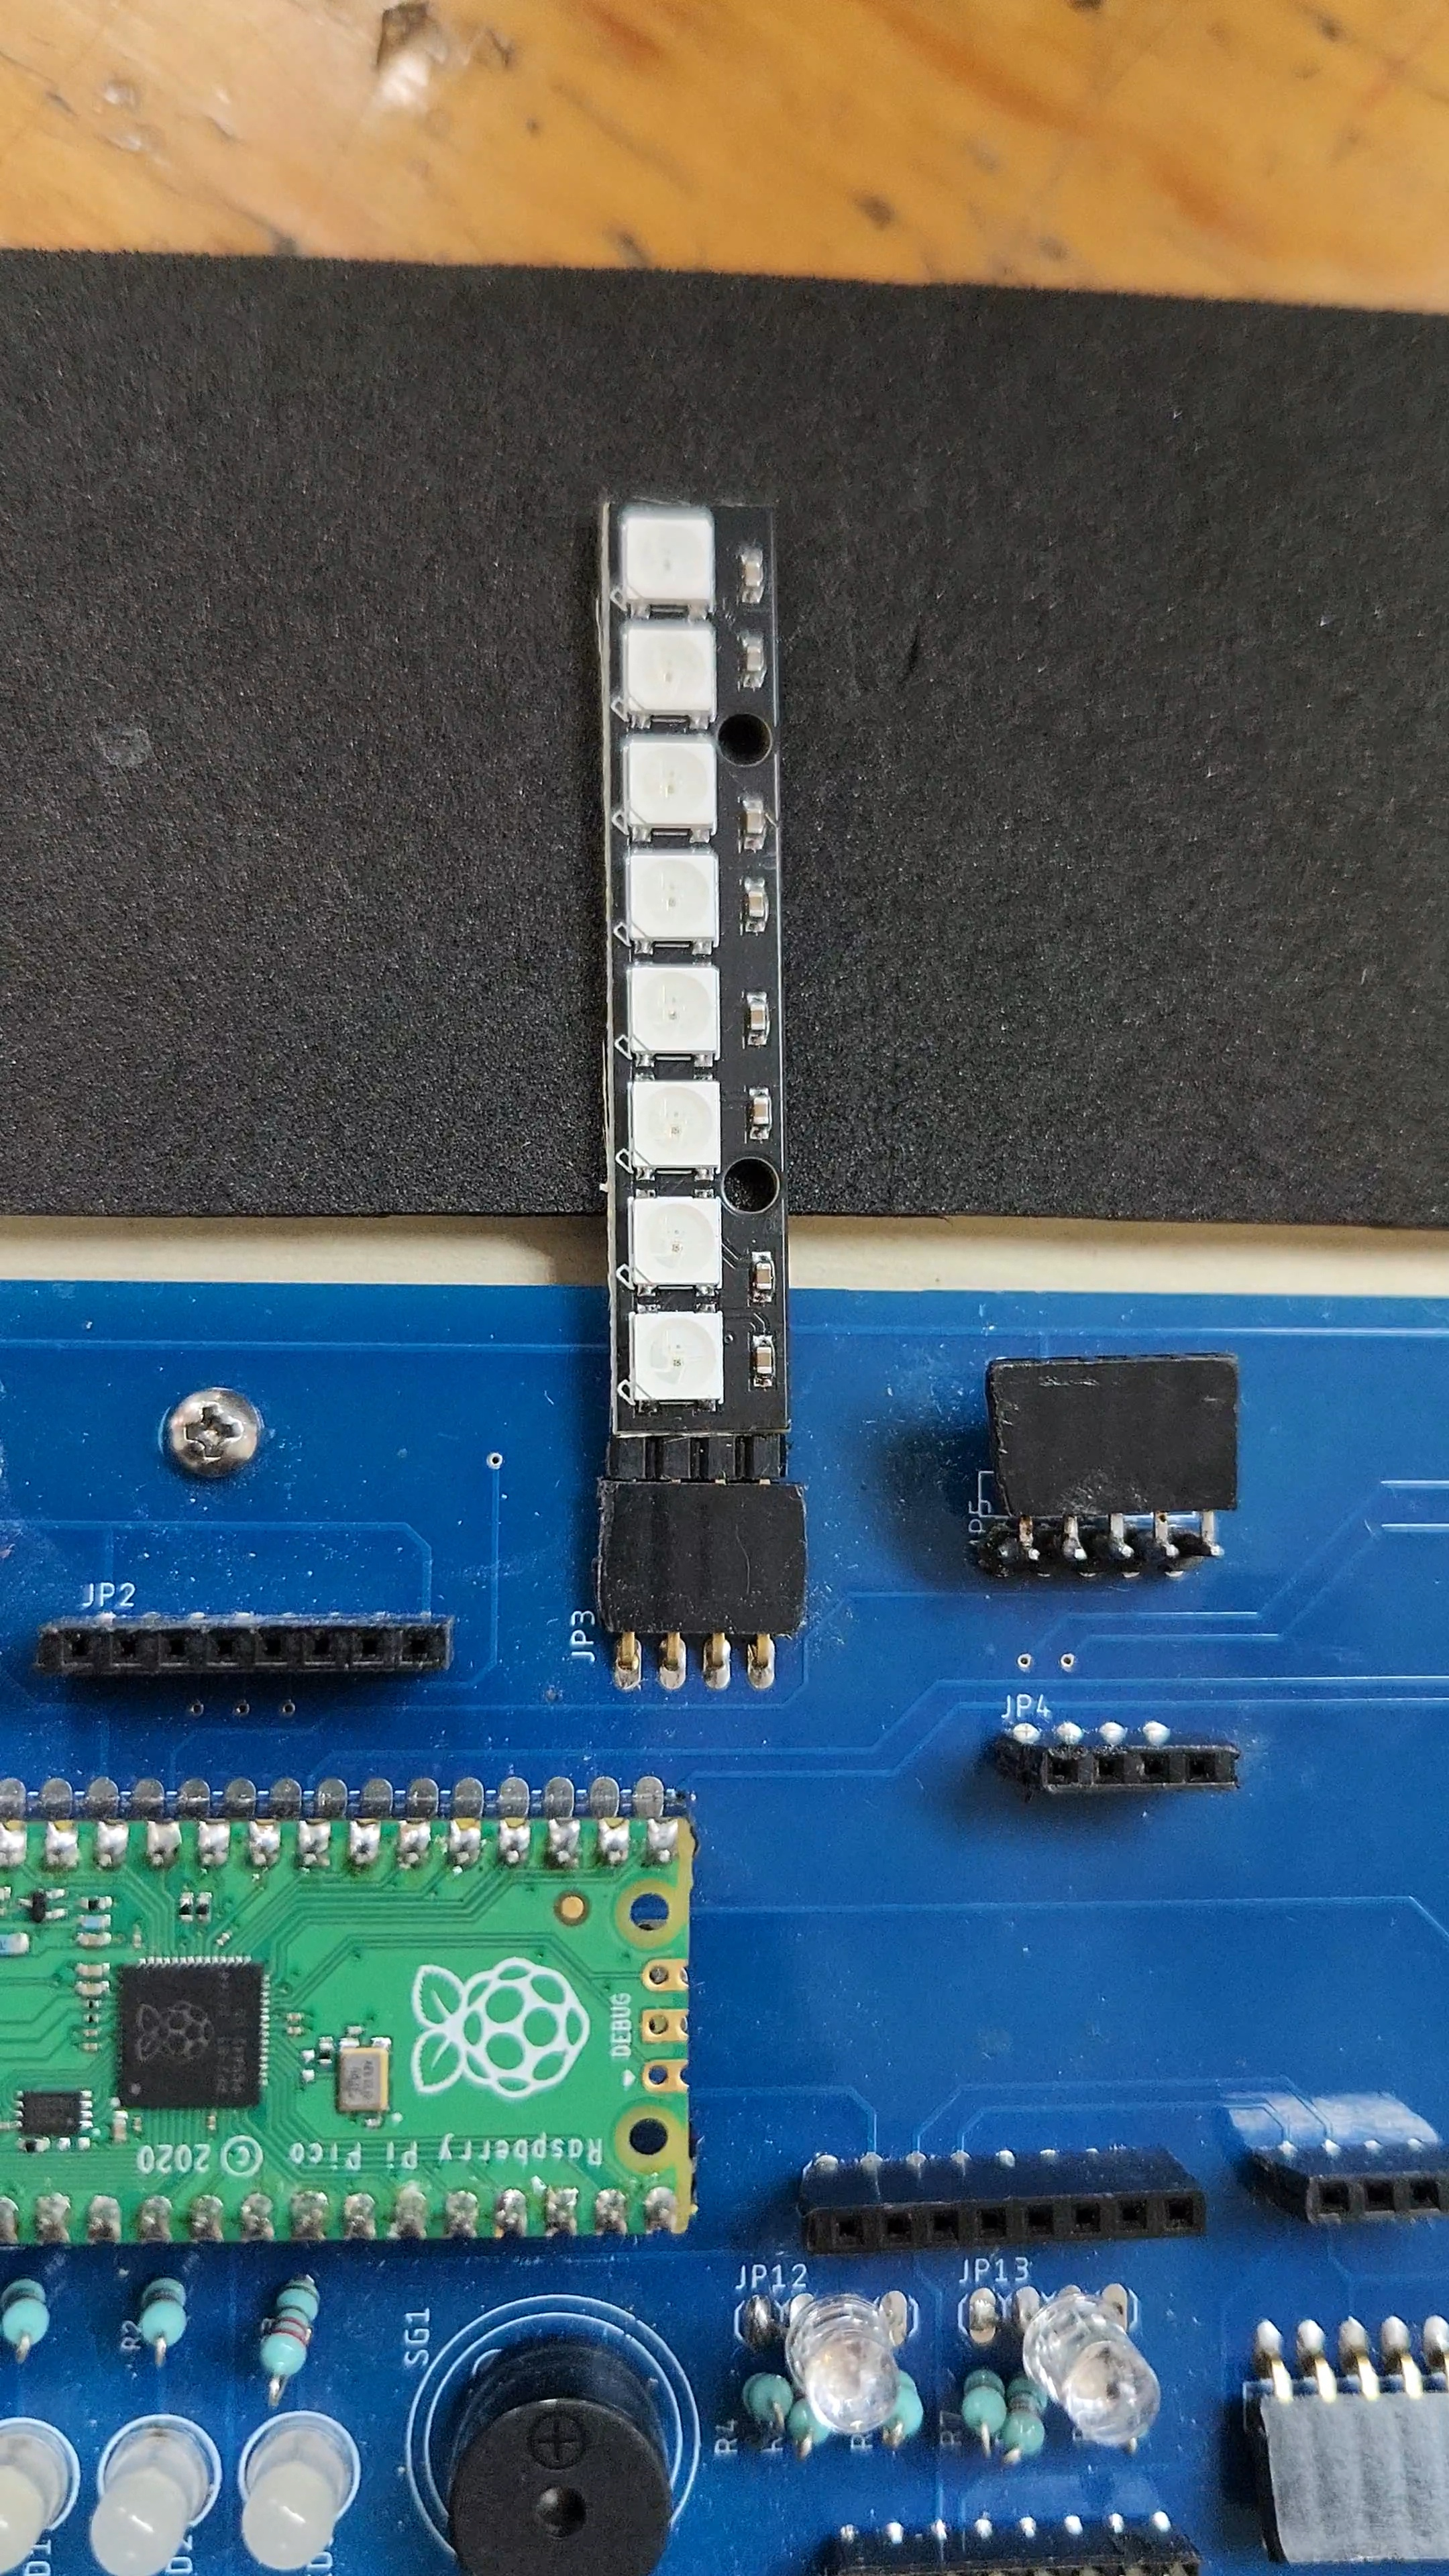
\includegraphics[width=0.25\textwidth, angle=90]{img/Actividad1/Act1_1.jpg}
    \caption{Conexión física de la Raspberry Pi Pico con la tira NeoPixel. Se observa la alimentación a 3.3V, la conexión a tierra (GND) y la línea de datos (DIN) conectada al pin GPIO 4.}
\end{figure}

\begin{figure}[H]
    \centering
    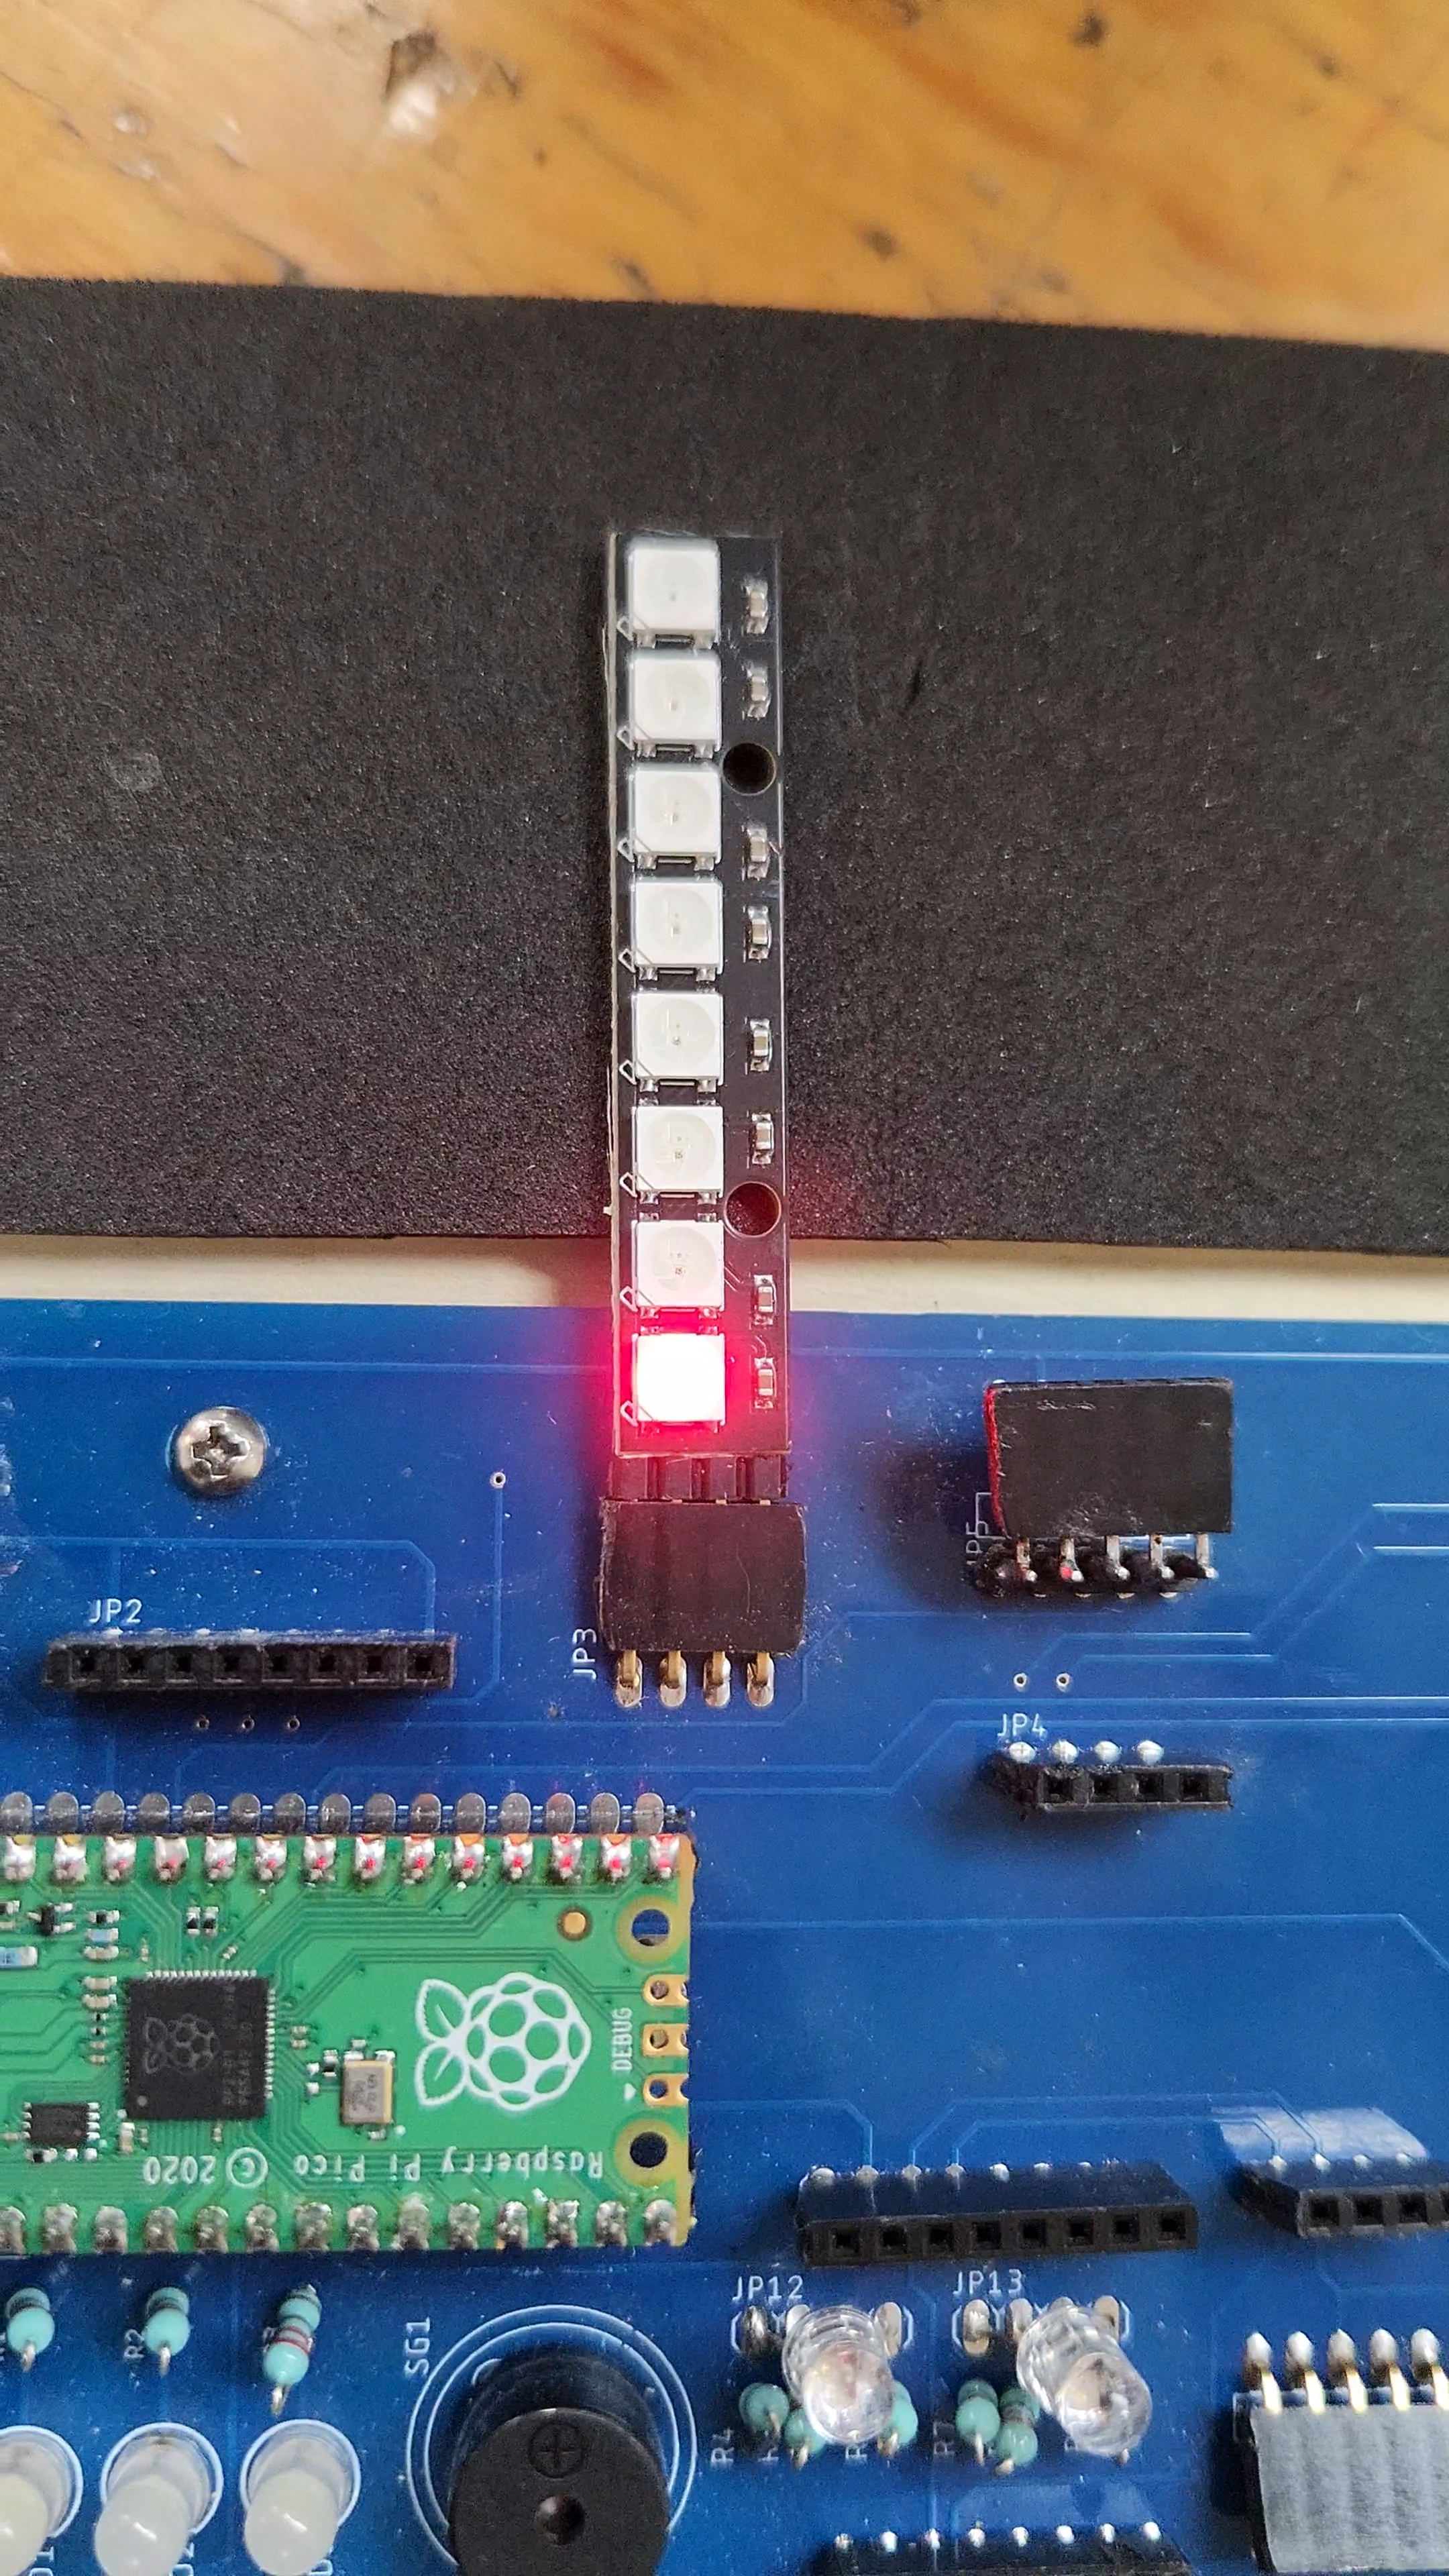
\includegraphics[width=0.25\textwidth, angle=90]{img/Actividad1/Act1_2.jpg}
    \caption{Secuencia de encendido del primer LED en color rojo. El LED ubicado en la posición 0 de la tira se enciende durante 1 segundo y se apaga durante otro segundo, generando un patrón de parpadeo continuo.}
\end{figure}

\subsection*{Análisis de resultados}

El programa implementa un ciclo infinito que enciende y apaga el primer LED de la tira NeoPixel cada segundo, generando un parpadeo constante que nos sirve para comprender mejor la libreria neopixel.

La libreria \texttt{neopixel} abstrae la complejidad del protocolo WS2812, generando automaticamente las señales mediante el subsistema PIO del RP2040. El uso de \texttt{brightness = 0.1} reduce el consumo de corriente a un nivel seguro para el puerto USB.

La secuencia \texttt{set\_pixel()} y \texttt{show()} asegura que los cambios se reflejen fisicamente, mientras que \texttt{time.sleep(1)} introduce una pausa para apreciar mejor el cambio.

    \newpage
   \section*{Actividad 2}

\noindent Utilizando la tira de 8 leds RGB; generar el efecto mostrado en la figura 9-11, en forma secuencial con tres distintos colores.

\vspace{1.5cm}

% Gráfico de la secuencia
\begin{center}
\begin{tikzpicture}
    % Definimos la secuencia de LEDs encendidos (Sube de 1 a 8 y baja de 8 a 1)
    \foreach \val [count=\i] in {1, 2, 3, 4, 5, 6, 7, 8, 7, 6, 5, 4, 3, 2, 1} {
        
        % Calculamos la posición en X para cada tira (0.85 de separación)
        \pgfmathsetmacro{\xoff}{(\i-1)*0.85}
        
        % Contorno principal de la tira de LEDs
        \draw[gray!80, thick] (\xoff, 0) rectangle (\xoff+0.6, 4.1);
        
        % Dibujamos los 8 LEDs individuales (de abajo hacia arriba)
        \foreach \j in {1,...,8} {
            % Calculamos la posición en Y
            \pgfmathsetmacro{\yoff}{(\j-1)*0.5 + 0.1}
            
            \ifnum\j>\val
                % Si el índice del LED es mayor que el valor de la secuencia -> APAGADO
                \draw[draw=gray!80, thick] (\xoff+0.1, \yoff) rectangle (\xoff+0.5, \yoff+0.35);
            \else
                % Si el índice del LED es menor o igual -> ENCENDIDO (Rojo)
                \draw[fill=red, draw=gray!80, thick] (\xoff+0.1, \yoff) rectangle (\xoff+0.5, \yoff+0.35);
            \fi
        }
    }
\end{tikzpicture}

\vspace{0.8cm}
% Pie de figura
{\sffamily Figura 9-11. Muestra de secuencia a generar; actividad 2}
\end{center}

\section*{Propuesta de solucion}

Para generar el efecto de barrido secuencial mostrado en la Figura 9-11, se utiliza la misma libreria \texttt{neopixel} documentada en la Actividad 1. La tira de 8 LEDs se conecta al pin GPIO 4. Se define una lista con tres colores (rojo, verde y azul). Por cada color, se ejecuta un bucle ascendente que enciende los LEDs desde la posicion 0 hasta la 7 con un retardo de 0.5 segundos entre cada encendido, logrando el efecto de llenado. Posteriormente, un bucle descendente apaga los LEDs desde la posicion 7 hasta la 0 con el mismo retardo, creando un efecto de vaciado que permite distinguir claramente la transicion entre colores.

\begin{center}
    \scalebox{0.82}{
    \begin{tikzpicture}[node distance=1.05cm, every node/.style={font=\scriptsize}]
        \node (start2) [startstop, text width=2.6cm] {Inicio};
        \node (init2) [process, below=of start2, text width=7.8cm] {Importar \texttt{time} y \texttt{Neopixel}. Configurar 8 LEDs en GPIO 4.};
        \node (colors2) [process, below=of init2, text width=6.5cm] {Definir \texttt{colores = [(255,0,0), (0,255,0), (0,0,255)]}.};
        \node (forcolor2) [process, below=of colors2, text width=4.8cm] {\texttt{for color in colores}: Iniciar};
        \node (fill2) [process, below=of forcolor2, text width=6.8cm] {\texttt{for i in range(8)}: \texttt{set\_pixel(i, color)}, \texttt{show()}, esperar 0.5 s};
        \node (clear2) [process, below=of fill2, text width=7.5cm] {\texttt{for i in range(8)}: \texttt{set\_pixel(7-i, (0,0,0))}, \texttt{show()}, esperar 0.5 s};
        \node (nextcolor2) [decision, below=of clear2, text width=3.8cm, aspect=2.2] {¿Quedan colores?};
        \node (repeat2) [decision, below=of nextcolor2, text width=3.5cm, aspect=2.2] {¿Repetir ciclo?};
        
        \draw [arrow] (start2) -- (init2);
        \draw [arrow] (init2) -- (colors2);
        \draw [arrow] (colors2) -- (forcolor2);
        \draw [arrow] (forcolor2) -- (fill2);
        \draw [arrow] (fill2) -- (clear2);
        \draw [arrow] (clear2) -- (nextcolor2);
        
        % Flecha "Si" para nextcolor2 (siguiente color)
        \draw [arrow] (nextcolor2.east) -- node[above, font=\scriptsize] {Si} ++(1.8,0) |- ([yshift=-0.3cm]forcolor2.east);
        
        % Flecha "No" para nextcolor2 (terminaron los colores)
        \draw [arrow] (nextcolor2.south) -- node[right, font=\scriptsize] {No} (repeat2);
        
        % Flecha "Si" para repeat2 (repetir todo el ciclo)
        \draw [arrow] (repeat2.west) -- node[above, font=\scriptsize] {Si} ++(-1.8,0) |- (forcolor2.west);
        
        % Flecha "No" para repeat2 (fin del programa)
        \draw [arrow] (repeat2.south) -- node[below, font=\scriptsize] {No} ++(0,-0.6) -- ++(0,0) node[below] {Fin};
        
    \end{tikzpicture}
    }
\end{center}

\section*{Desarrollo}

\lstinputlisting[language={[LAB]Python}, caption=Codigo de la Actividad 2, basicstyle=\ttfamily\scriptsize]{Code/Act2.py}

% ==========================================
% BLOQUE 1: Color Rojo (15 imagenes)
% ==========================================
\textbf{Secuencia en color rojo}

\begin{figure}[H]
    \centering
    \begin{minipage}{0.3\textwidth}
        \centering
        
\includegraphics[width=\textwidth]{img/Actividad2/Act2_2.jpg}
        \caption{Posicion 1}
    \end{minipage}\hfill
    \begin{minipage}{0.3\textwidth}
        \centering
        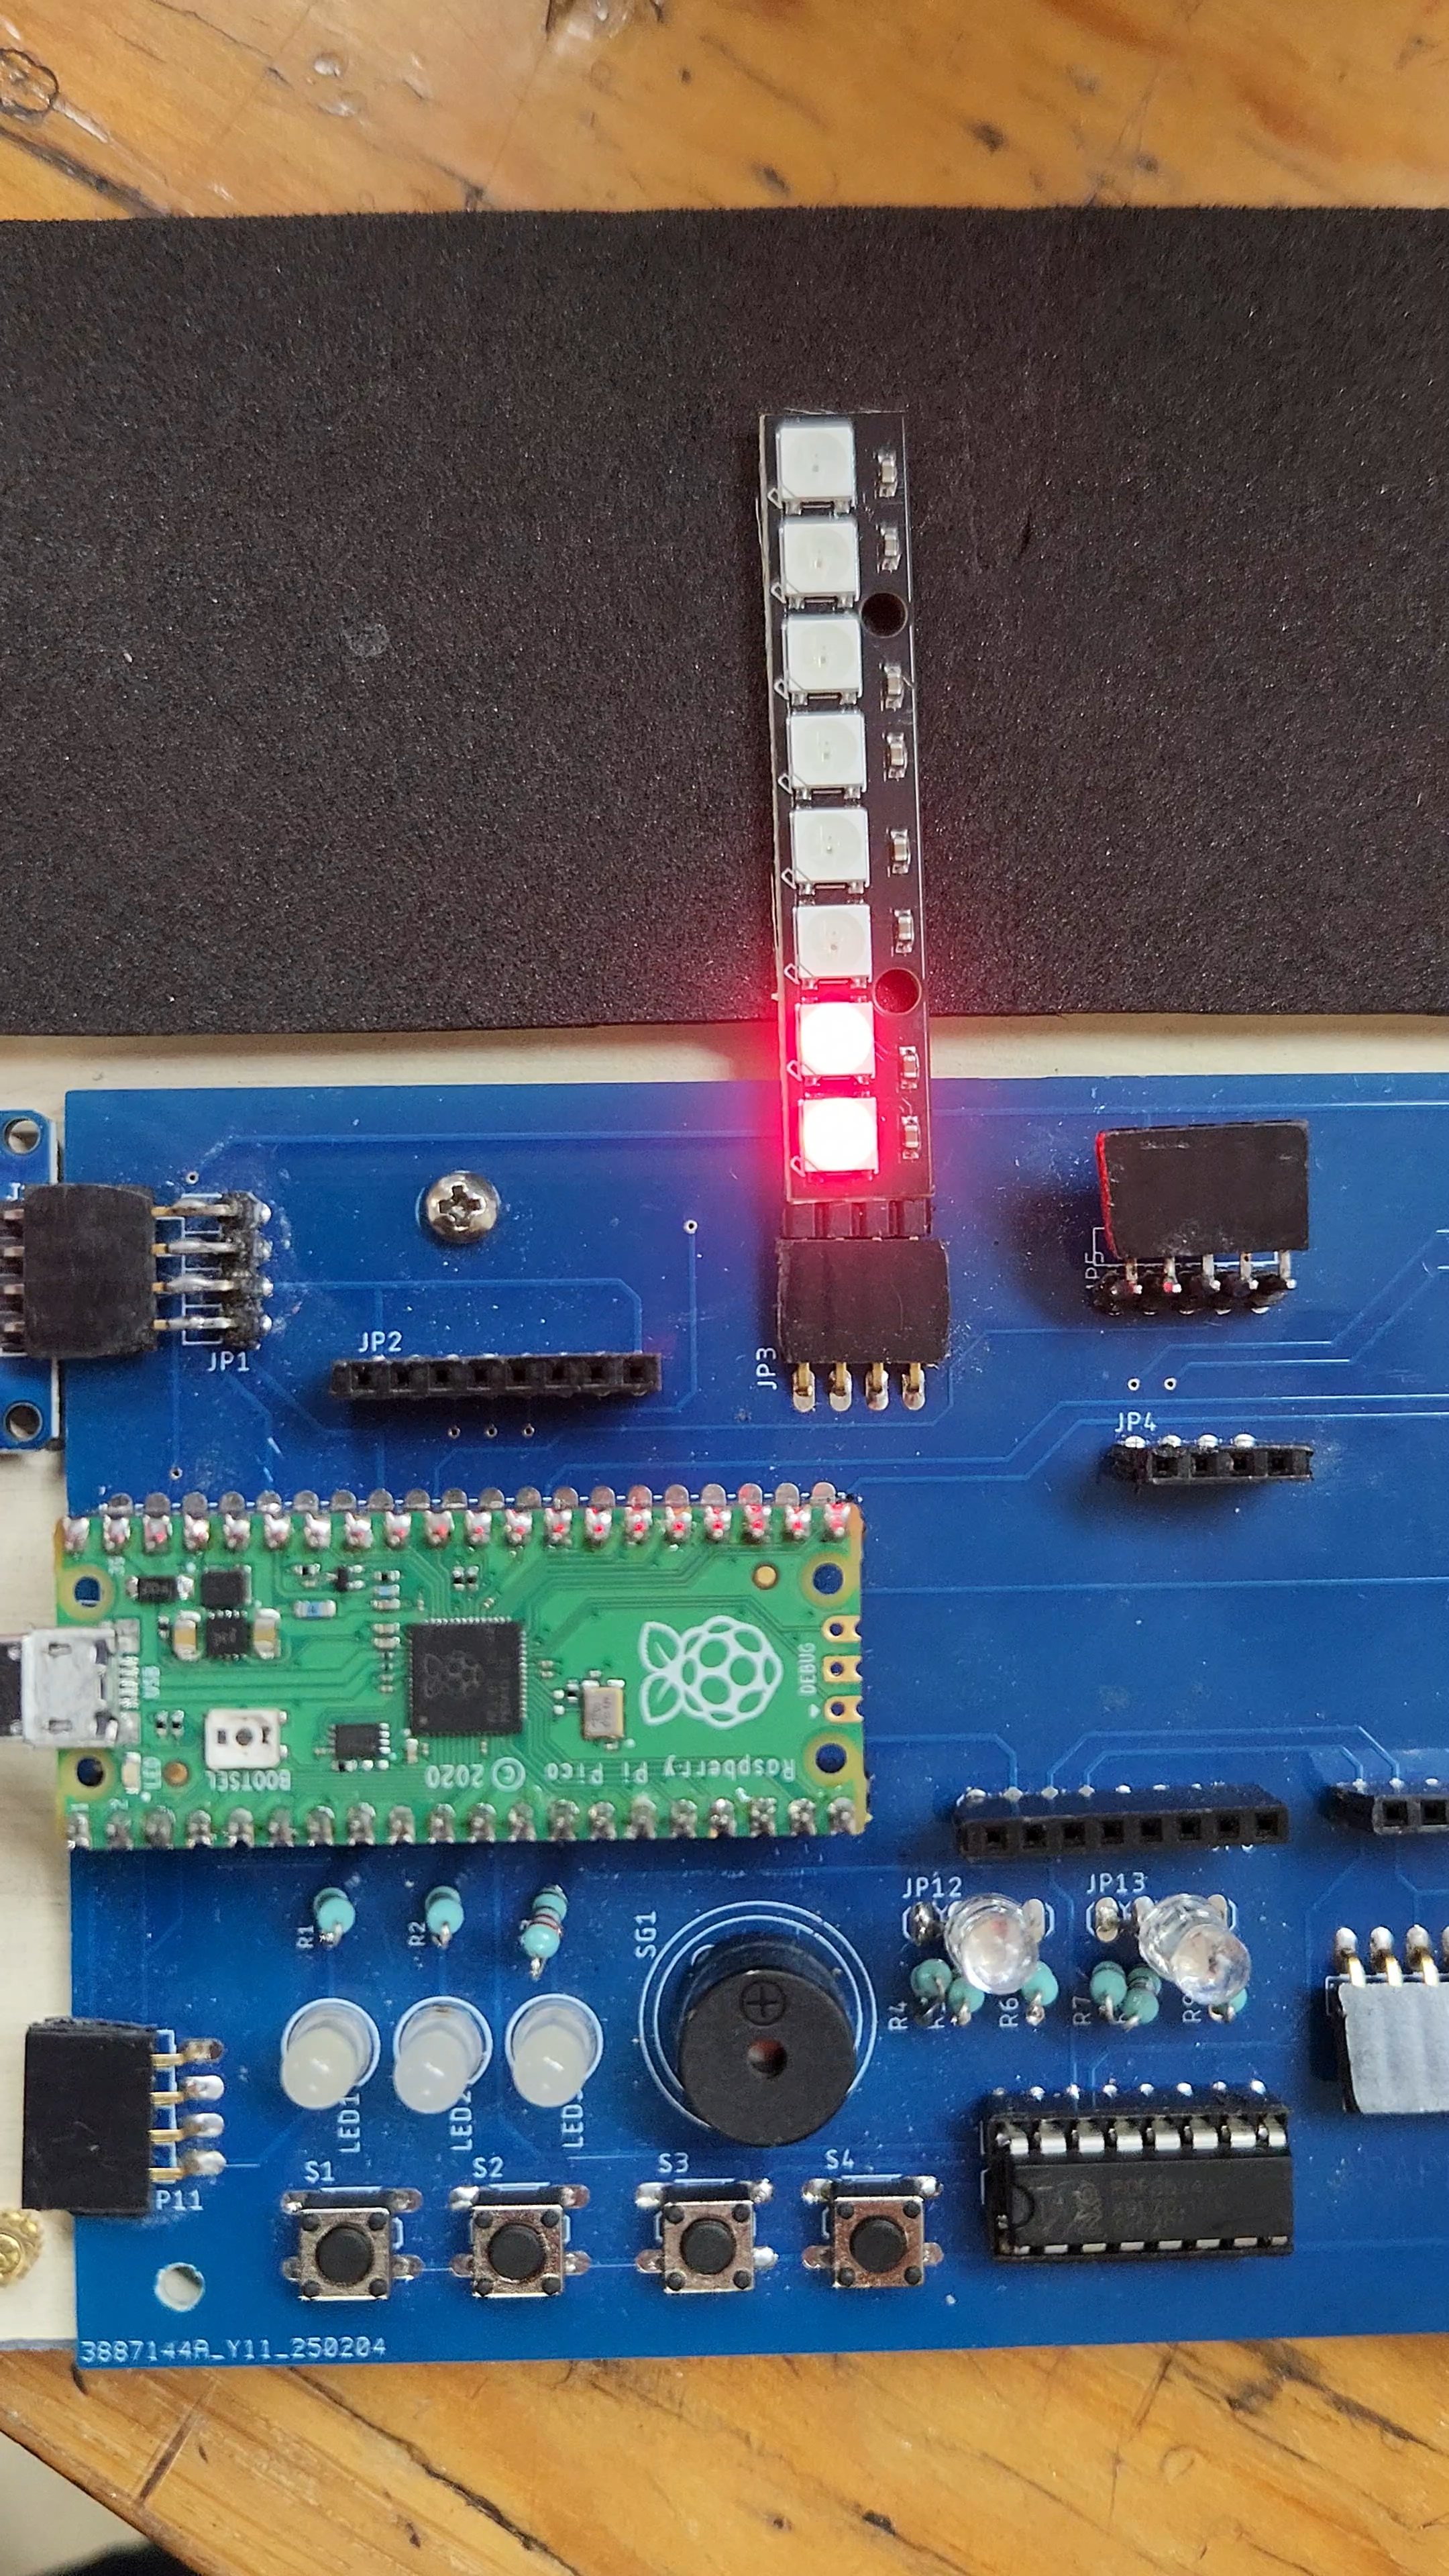
\includegraphics[width=\textwidth]{img/Actividad2/Act2_20.jpg}
        \caption{Posicion 2}
    \end{minipage}\hfill
    \begin{minipage}{0.3\textwidth}
        \centering
        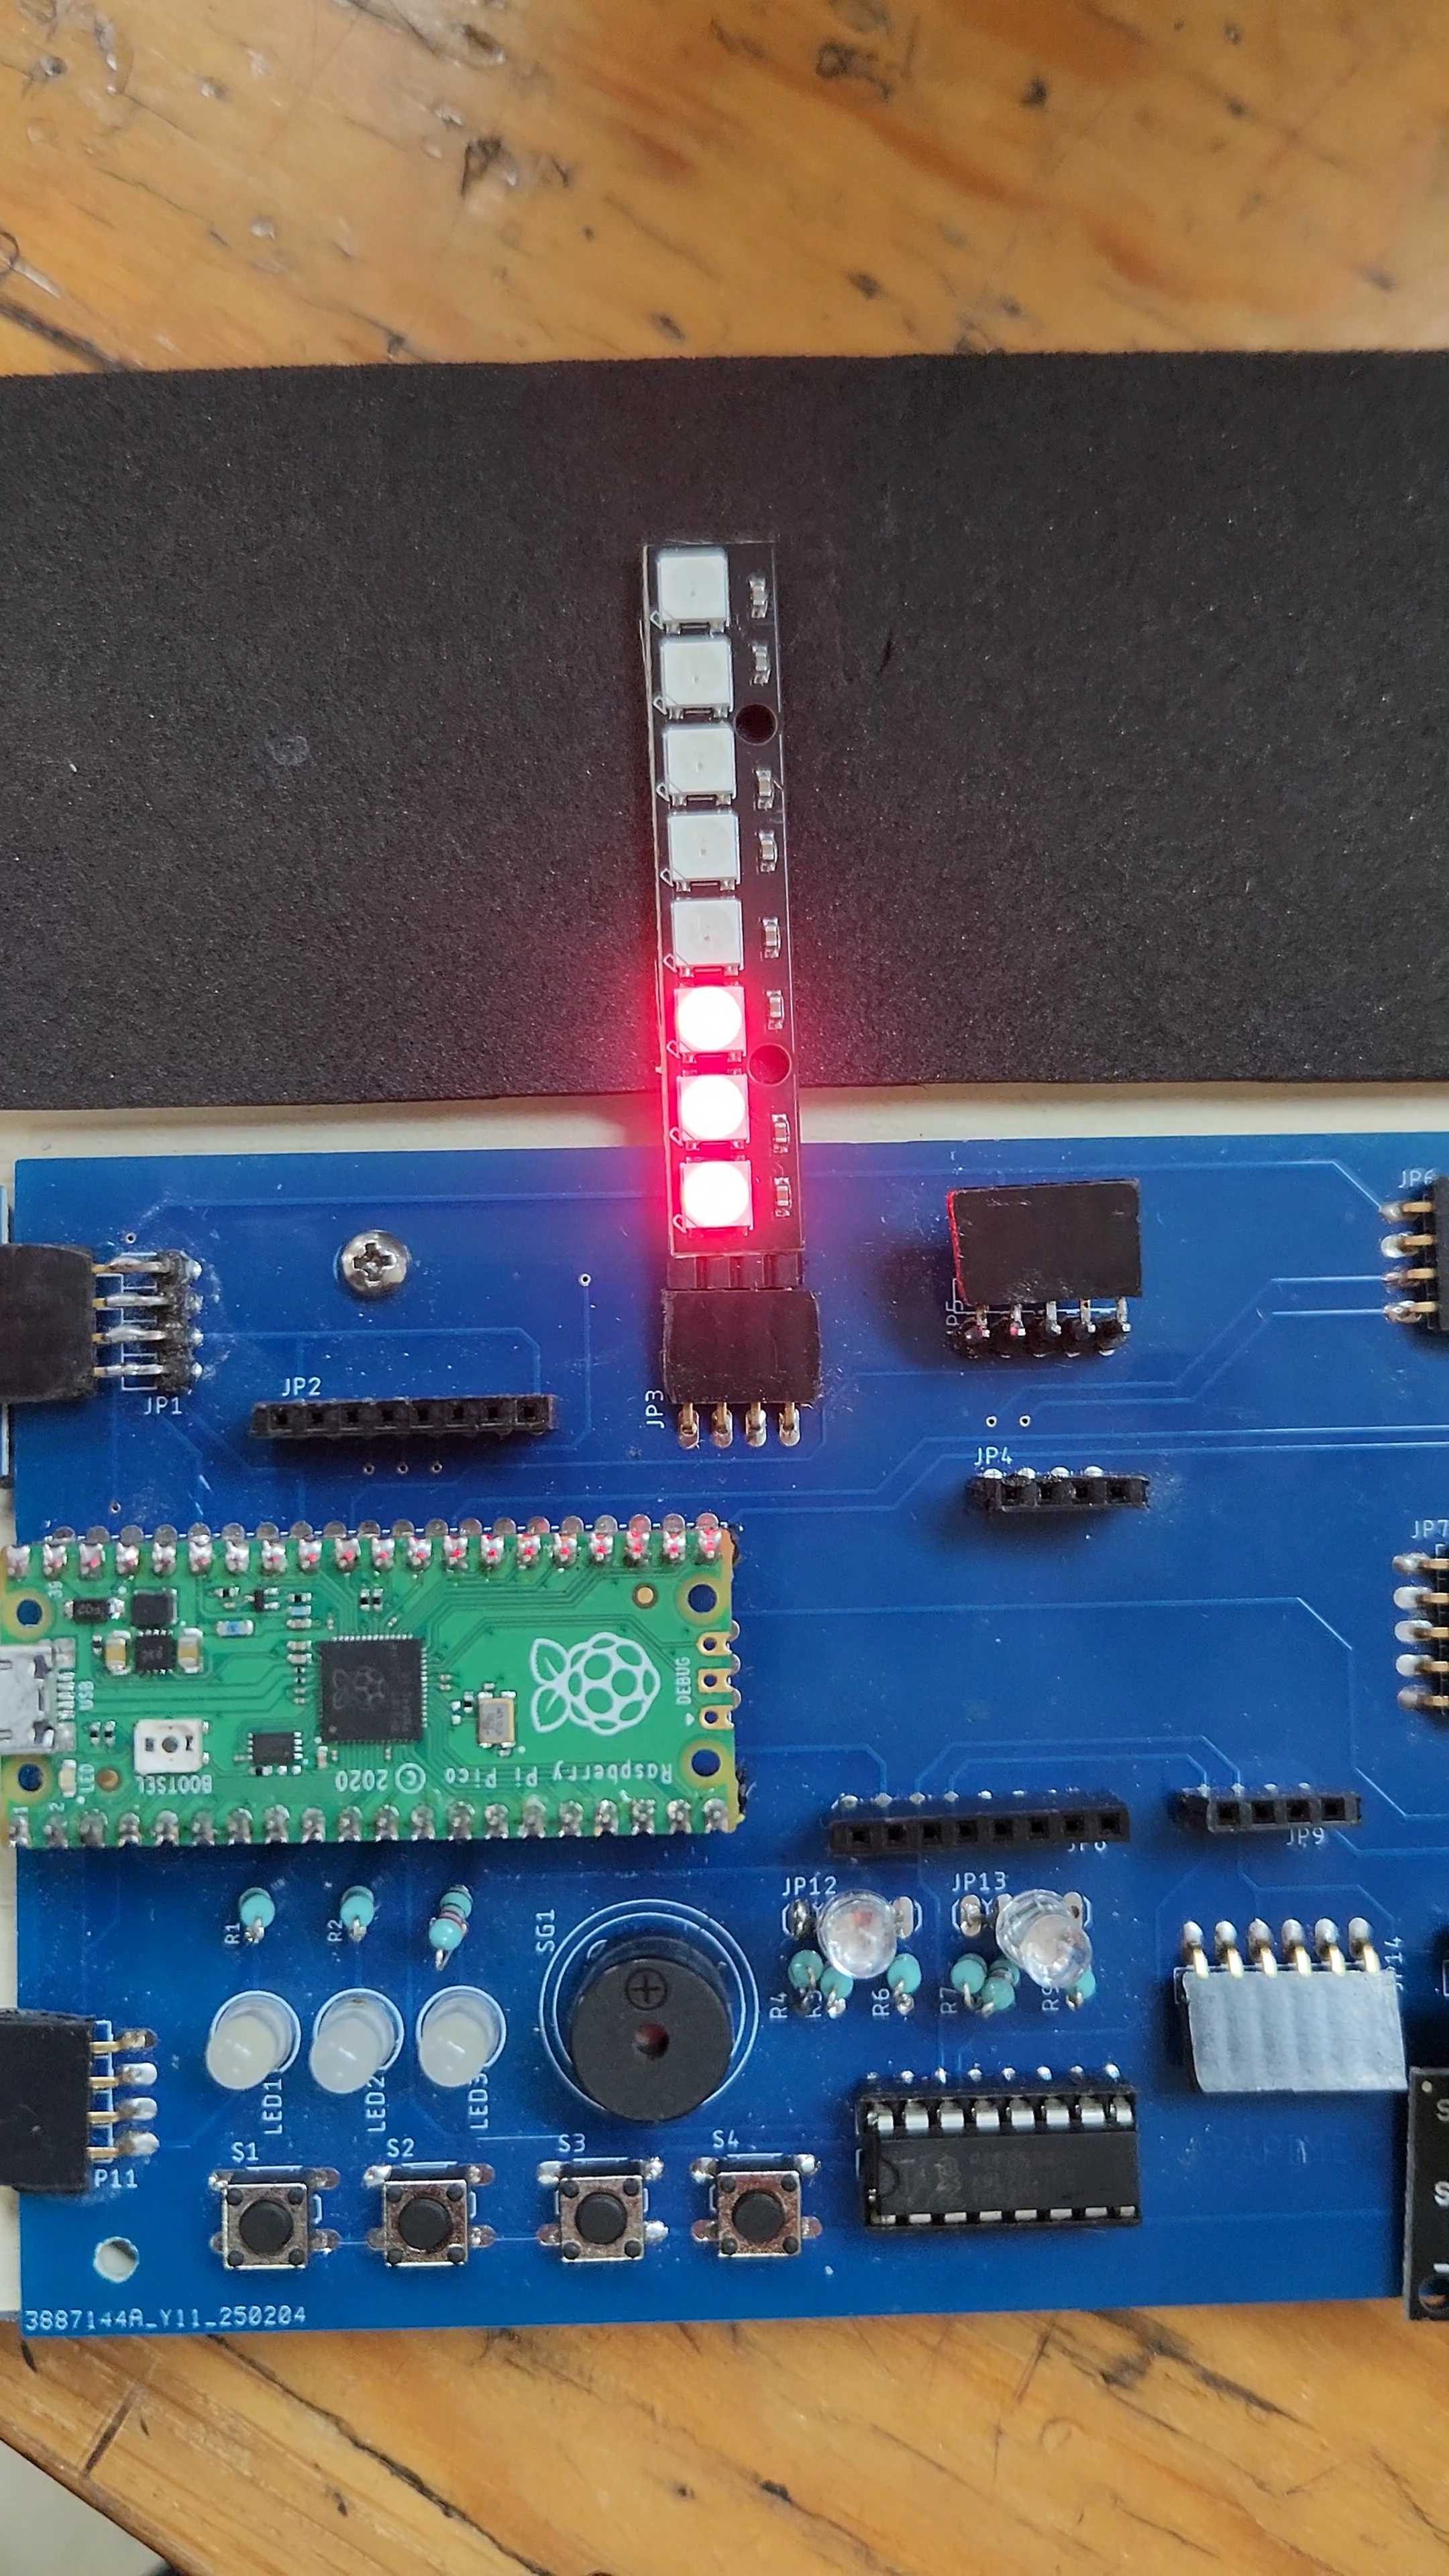
\includegraphics[width=\textwidth]{img/Actividad2/Act2_27.jpg}
        \caption{Posicion 3}
    \end{minipage}
\end{figure}

\begin{figure}[H]
    \centering
    \begin{minipage}{0.3\textwidth}
        \centering
        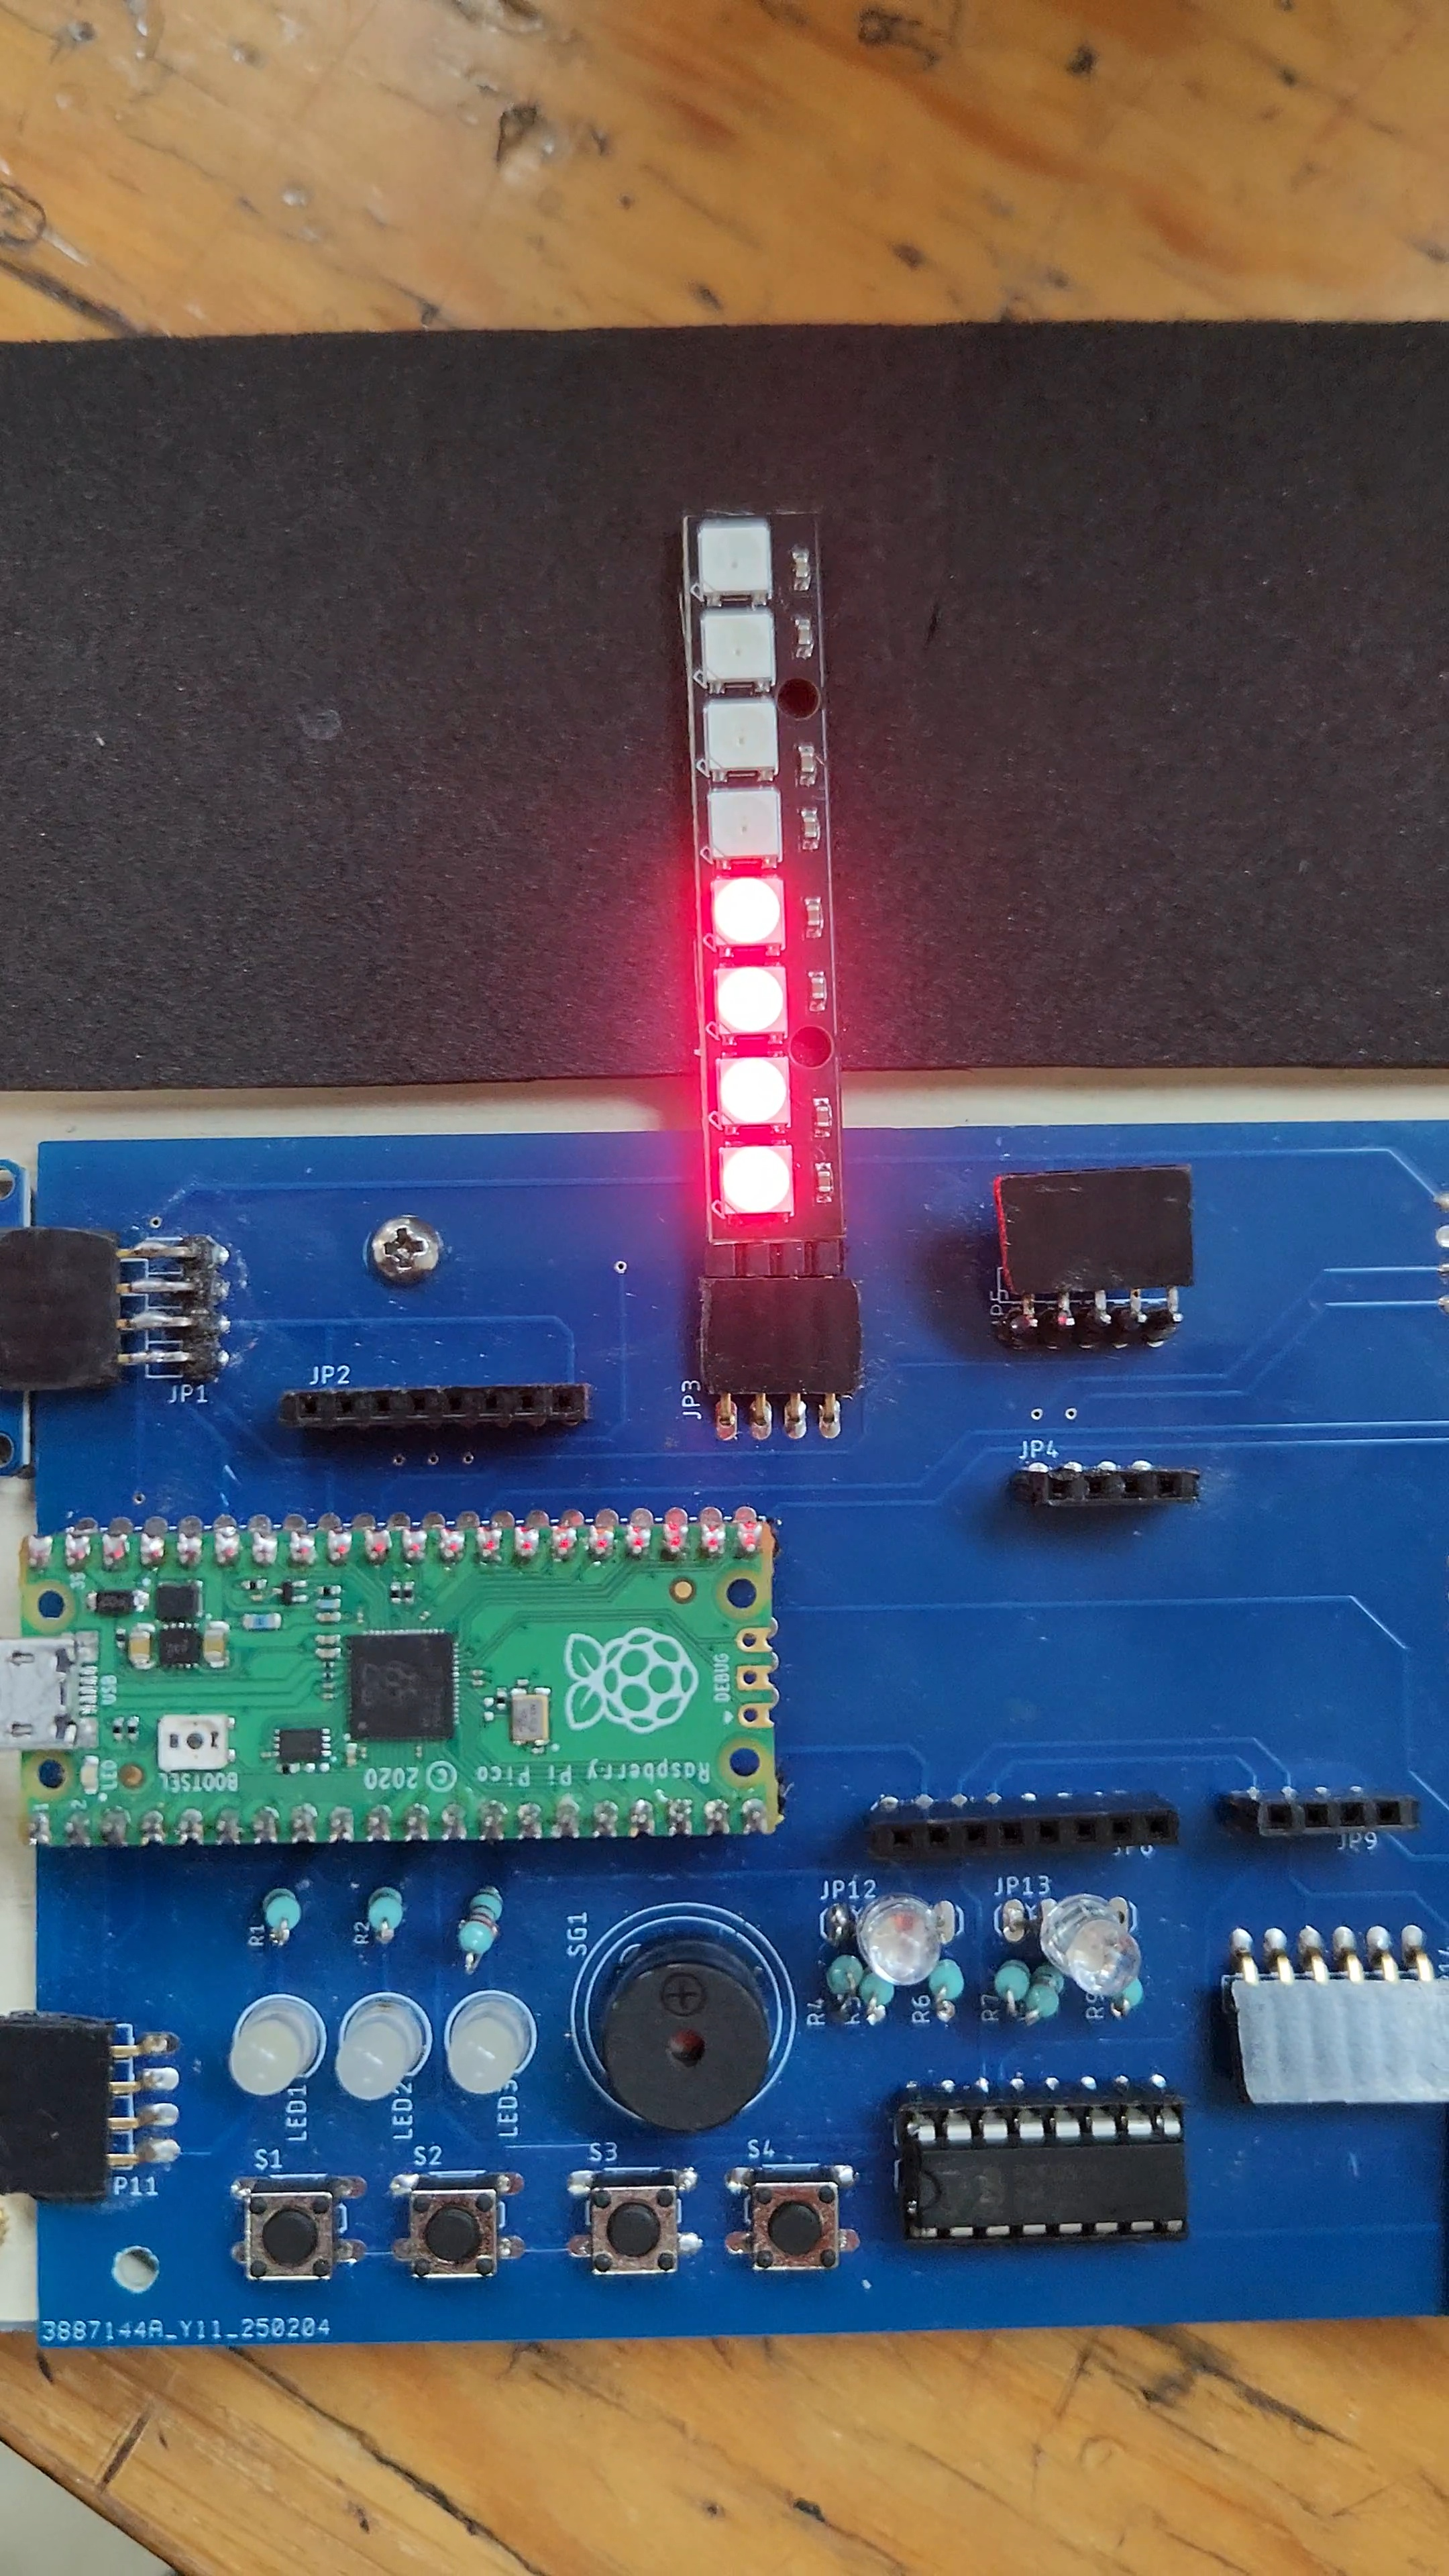
\includegraphics[width=\textwidth]{img/Actividad2/Act2_26.jpg}
        \caption{Posicion 4}
    \end{minipage}\hfill
    \begin{minipage}{0.3\textwidth}
        \centering
        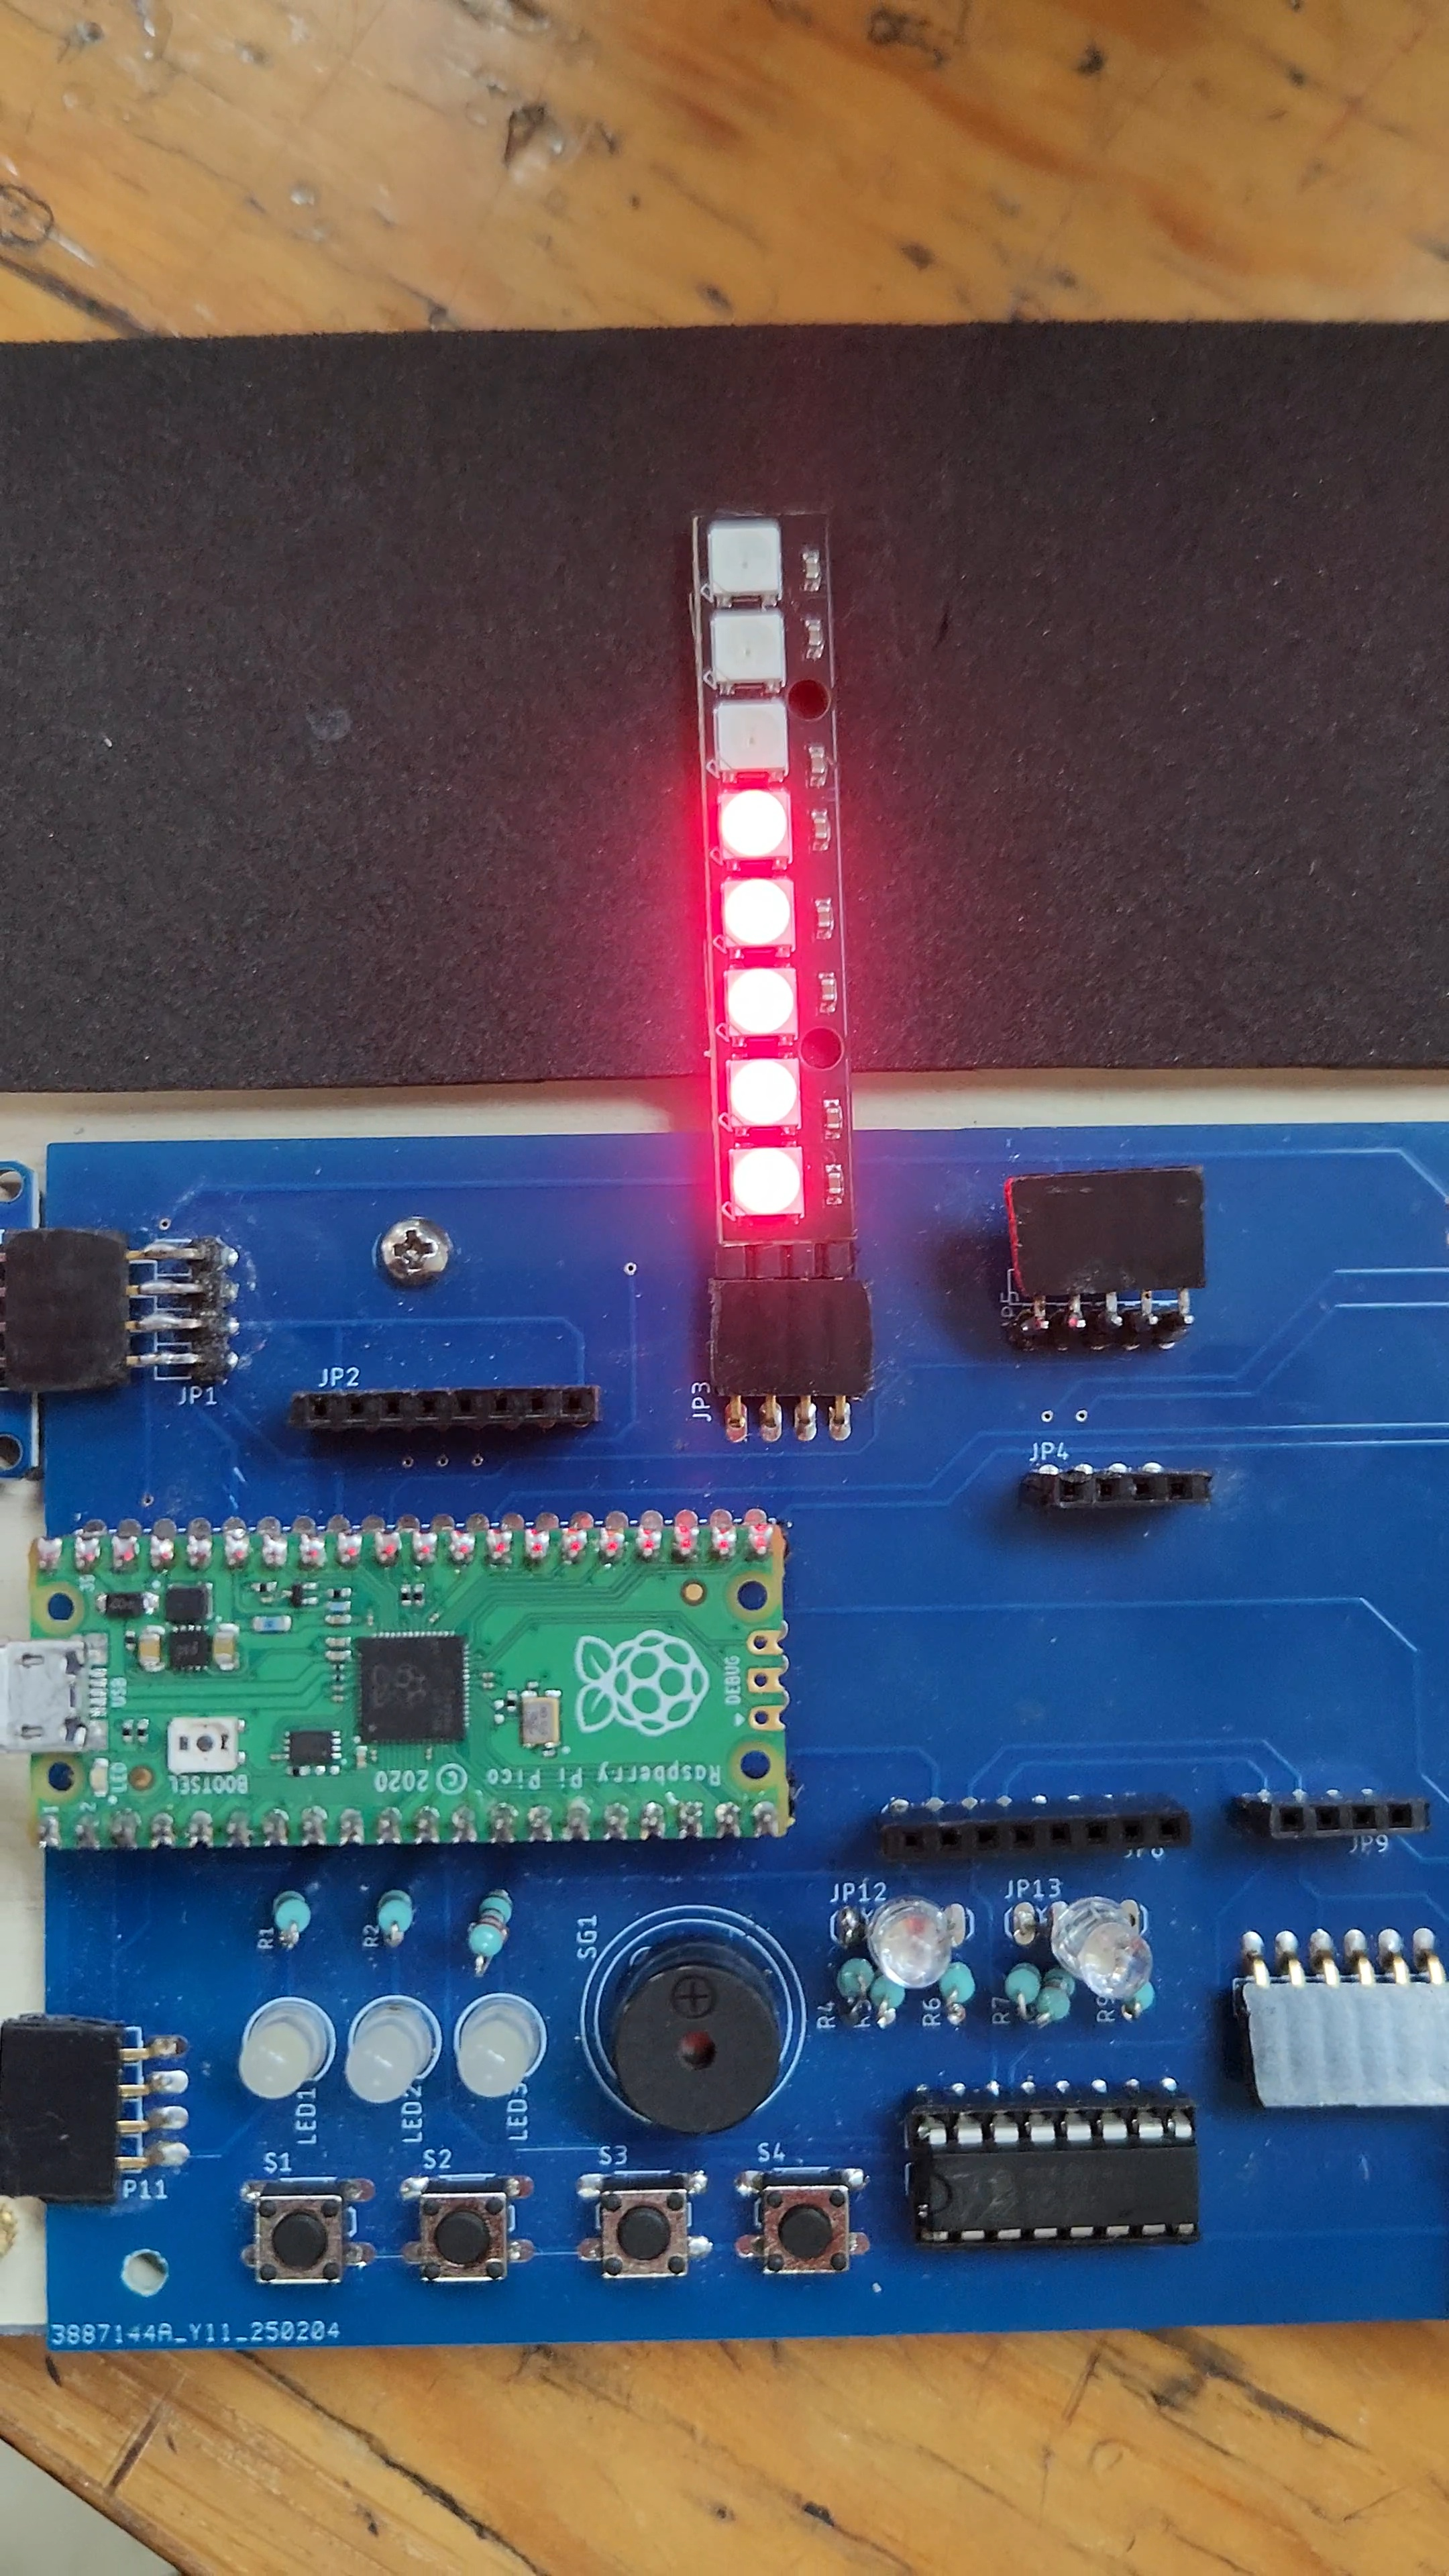
\includegraphics[width=\textwidth]{img/Actividad2/Act2_25.jpg}
        \caption{Posicion 5}
    \end{minipage}\hfill
    \begin{minipage}{0.3\textwidth}
        \centering
        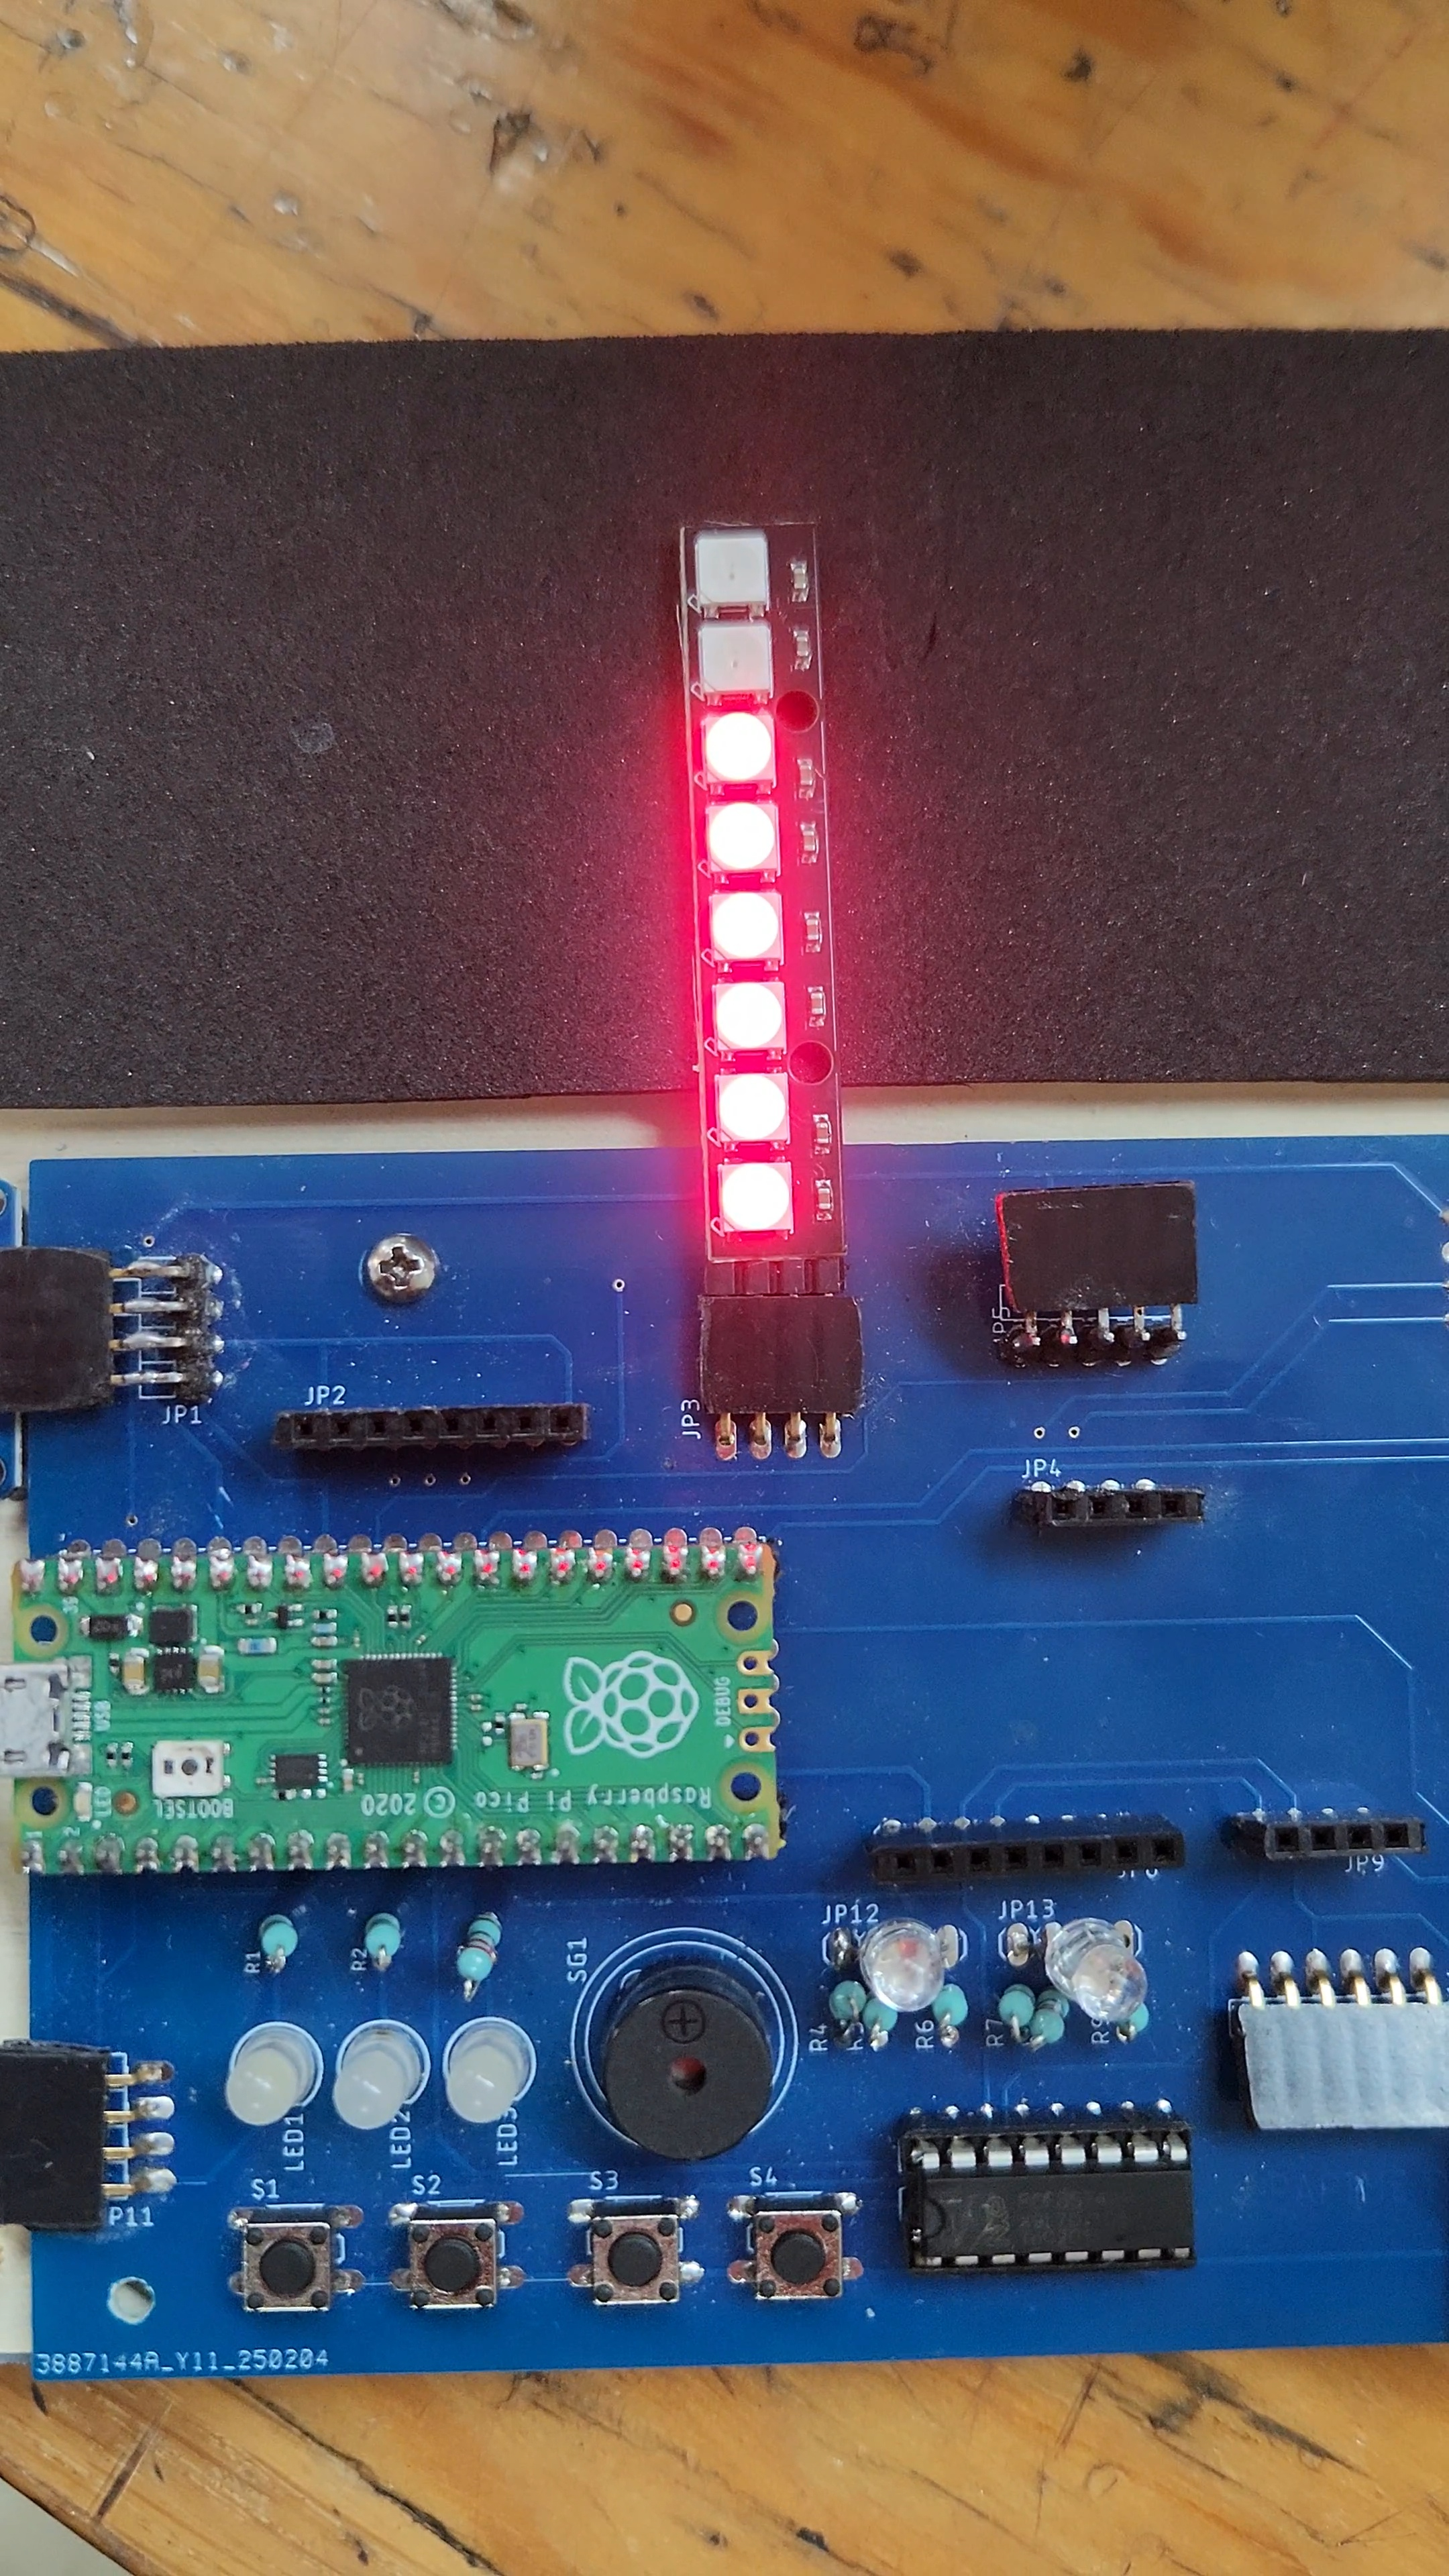
\includegraphics[width=\textwidth]{img/Actividad2/Act2_24.jpg}
        \caption{Posicion 6}
    \end{minipage}
\end{figure}

\begin{figure}[H]
    \centering
    \begin{minipage}{0.3\textwidth}
        \centering
        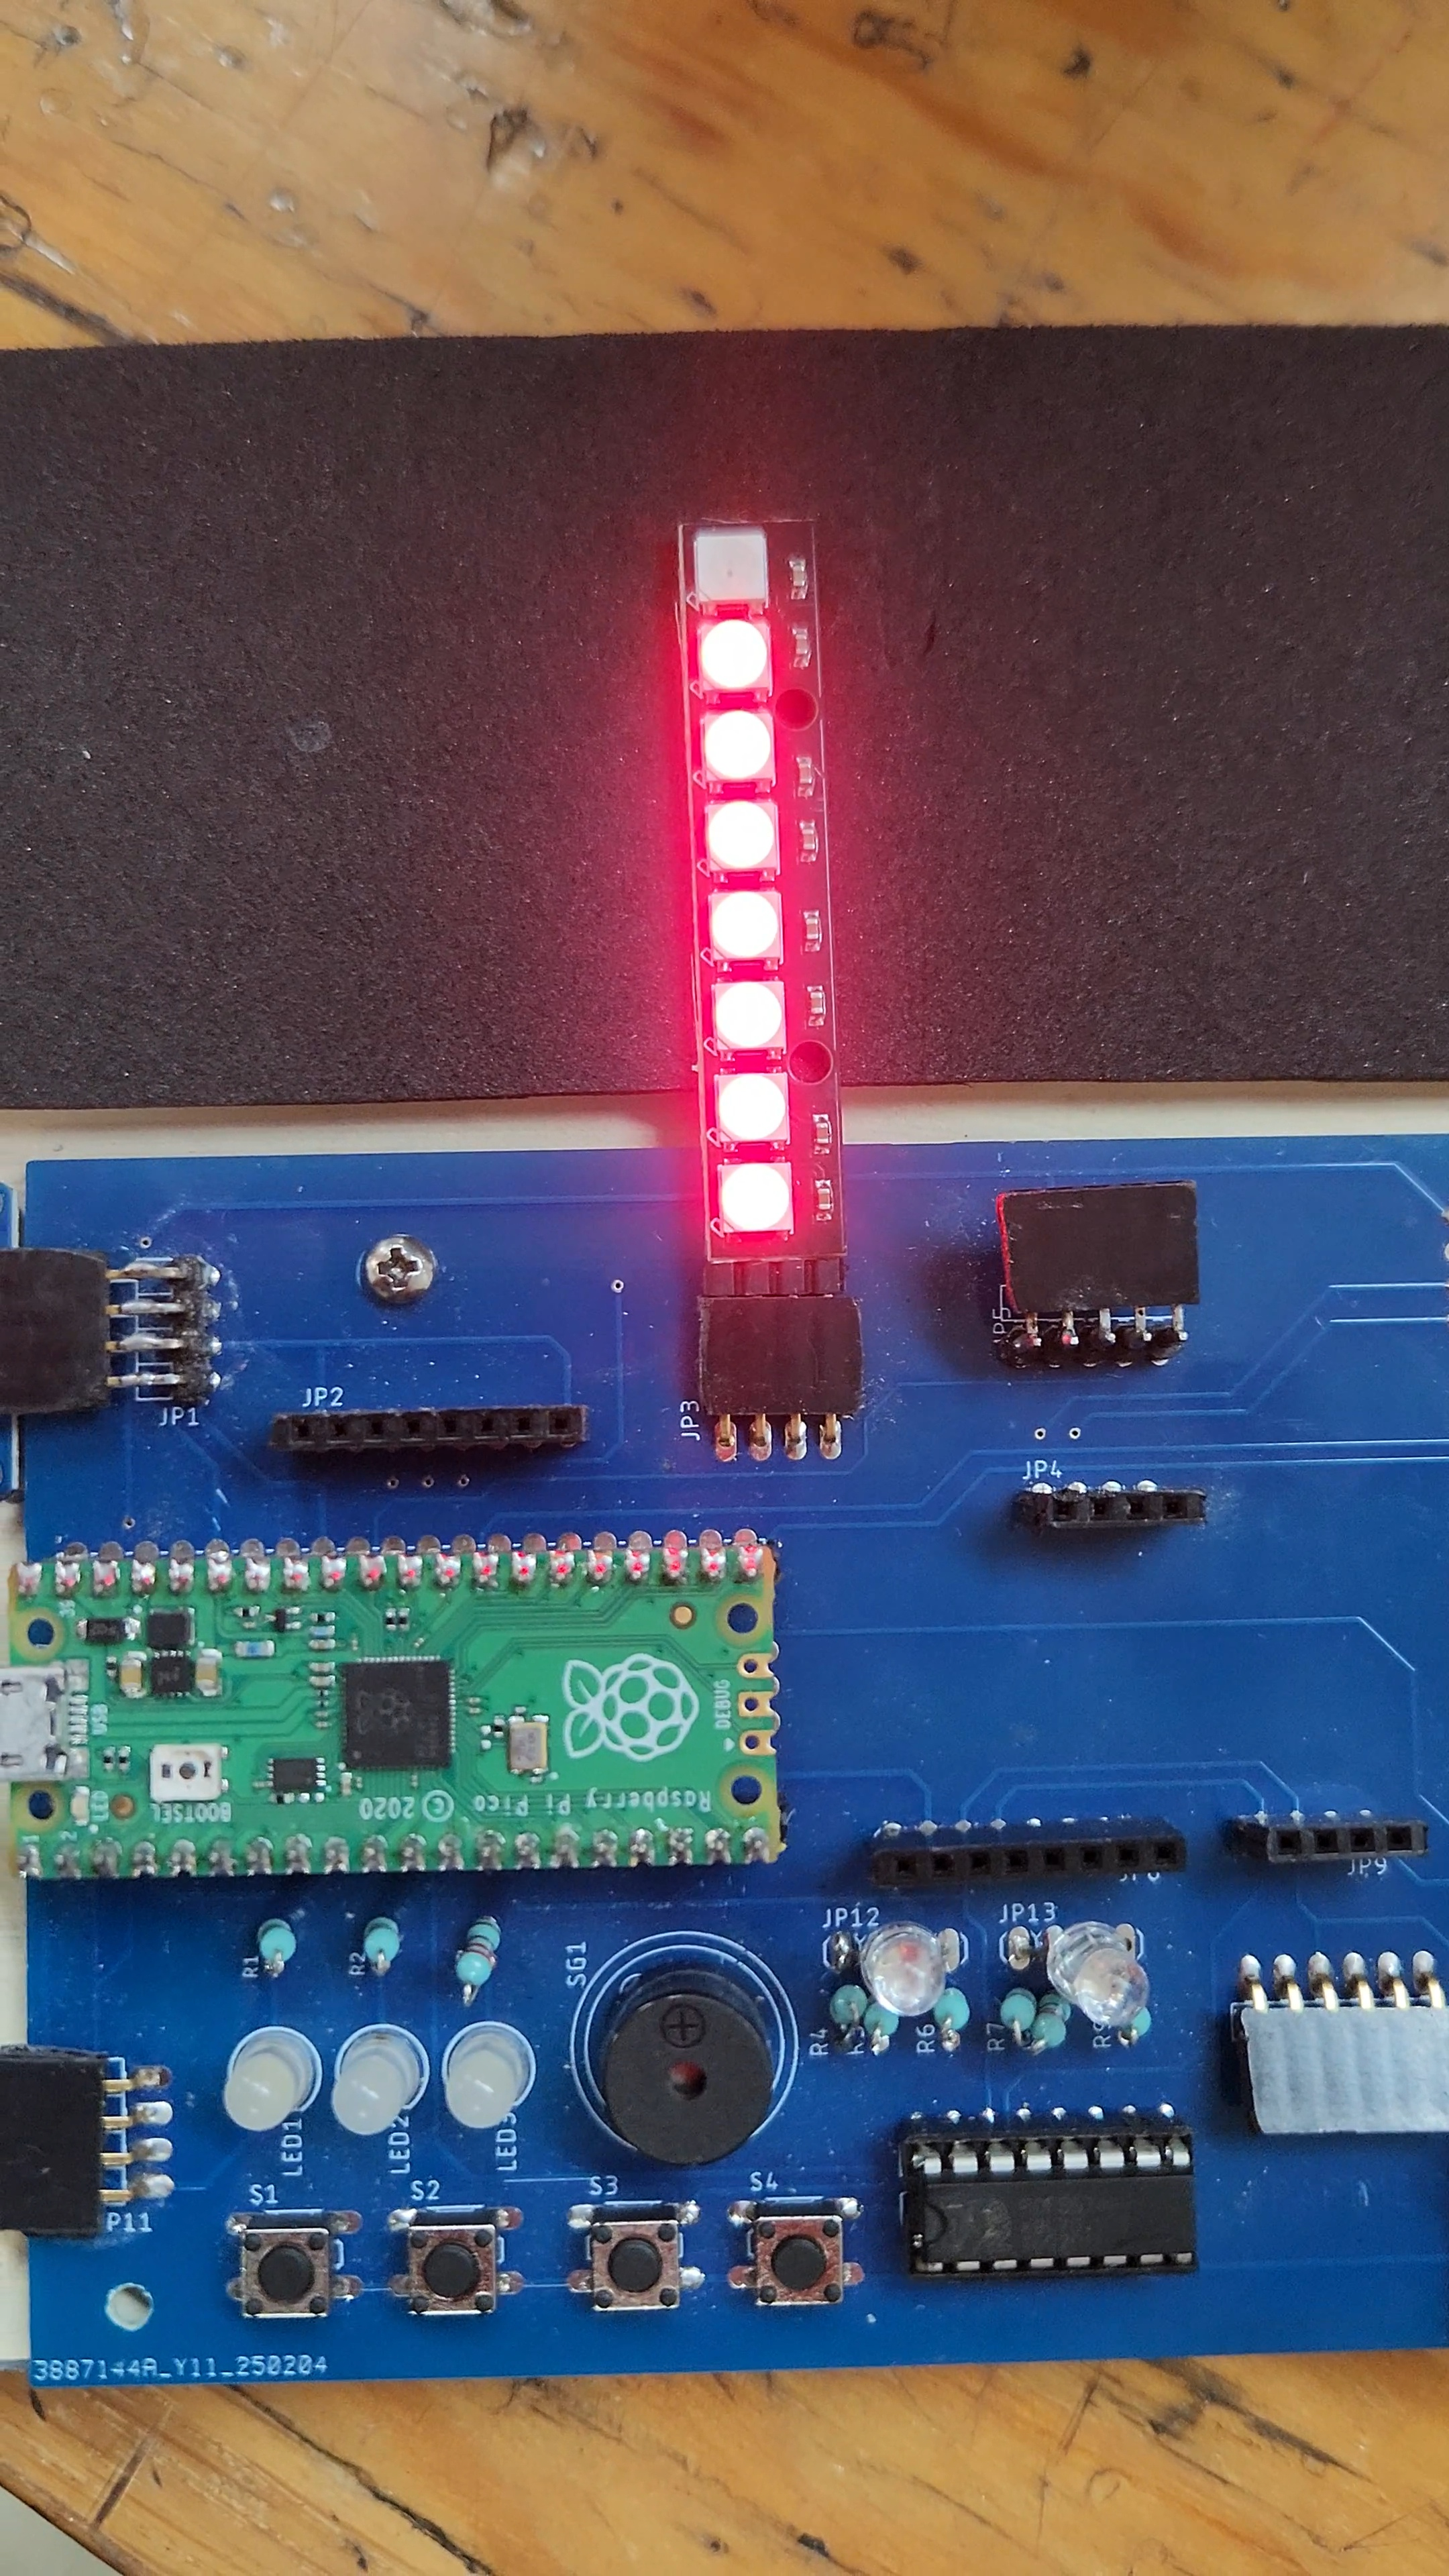
\includegraphics[width=\textwidth]{img/Actividad2/Act2_23.jpg}
        \caption{Posicion 7}
    \end{minipage}\hfill
    \begin{minipage}{0.3\textwidth}
        \centering
        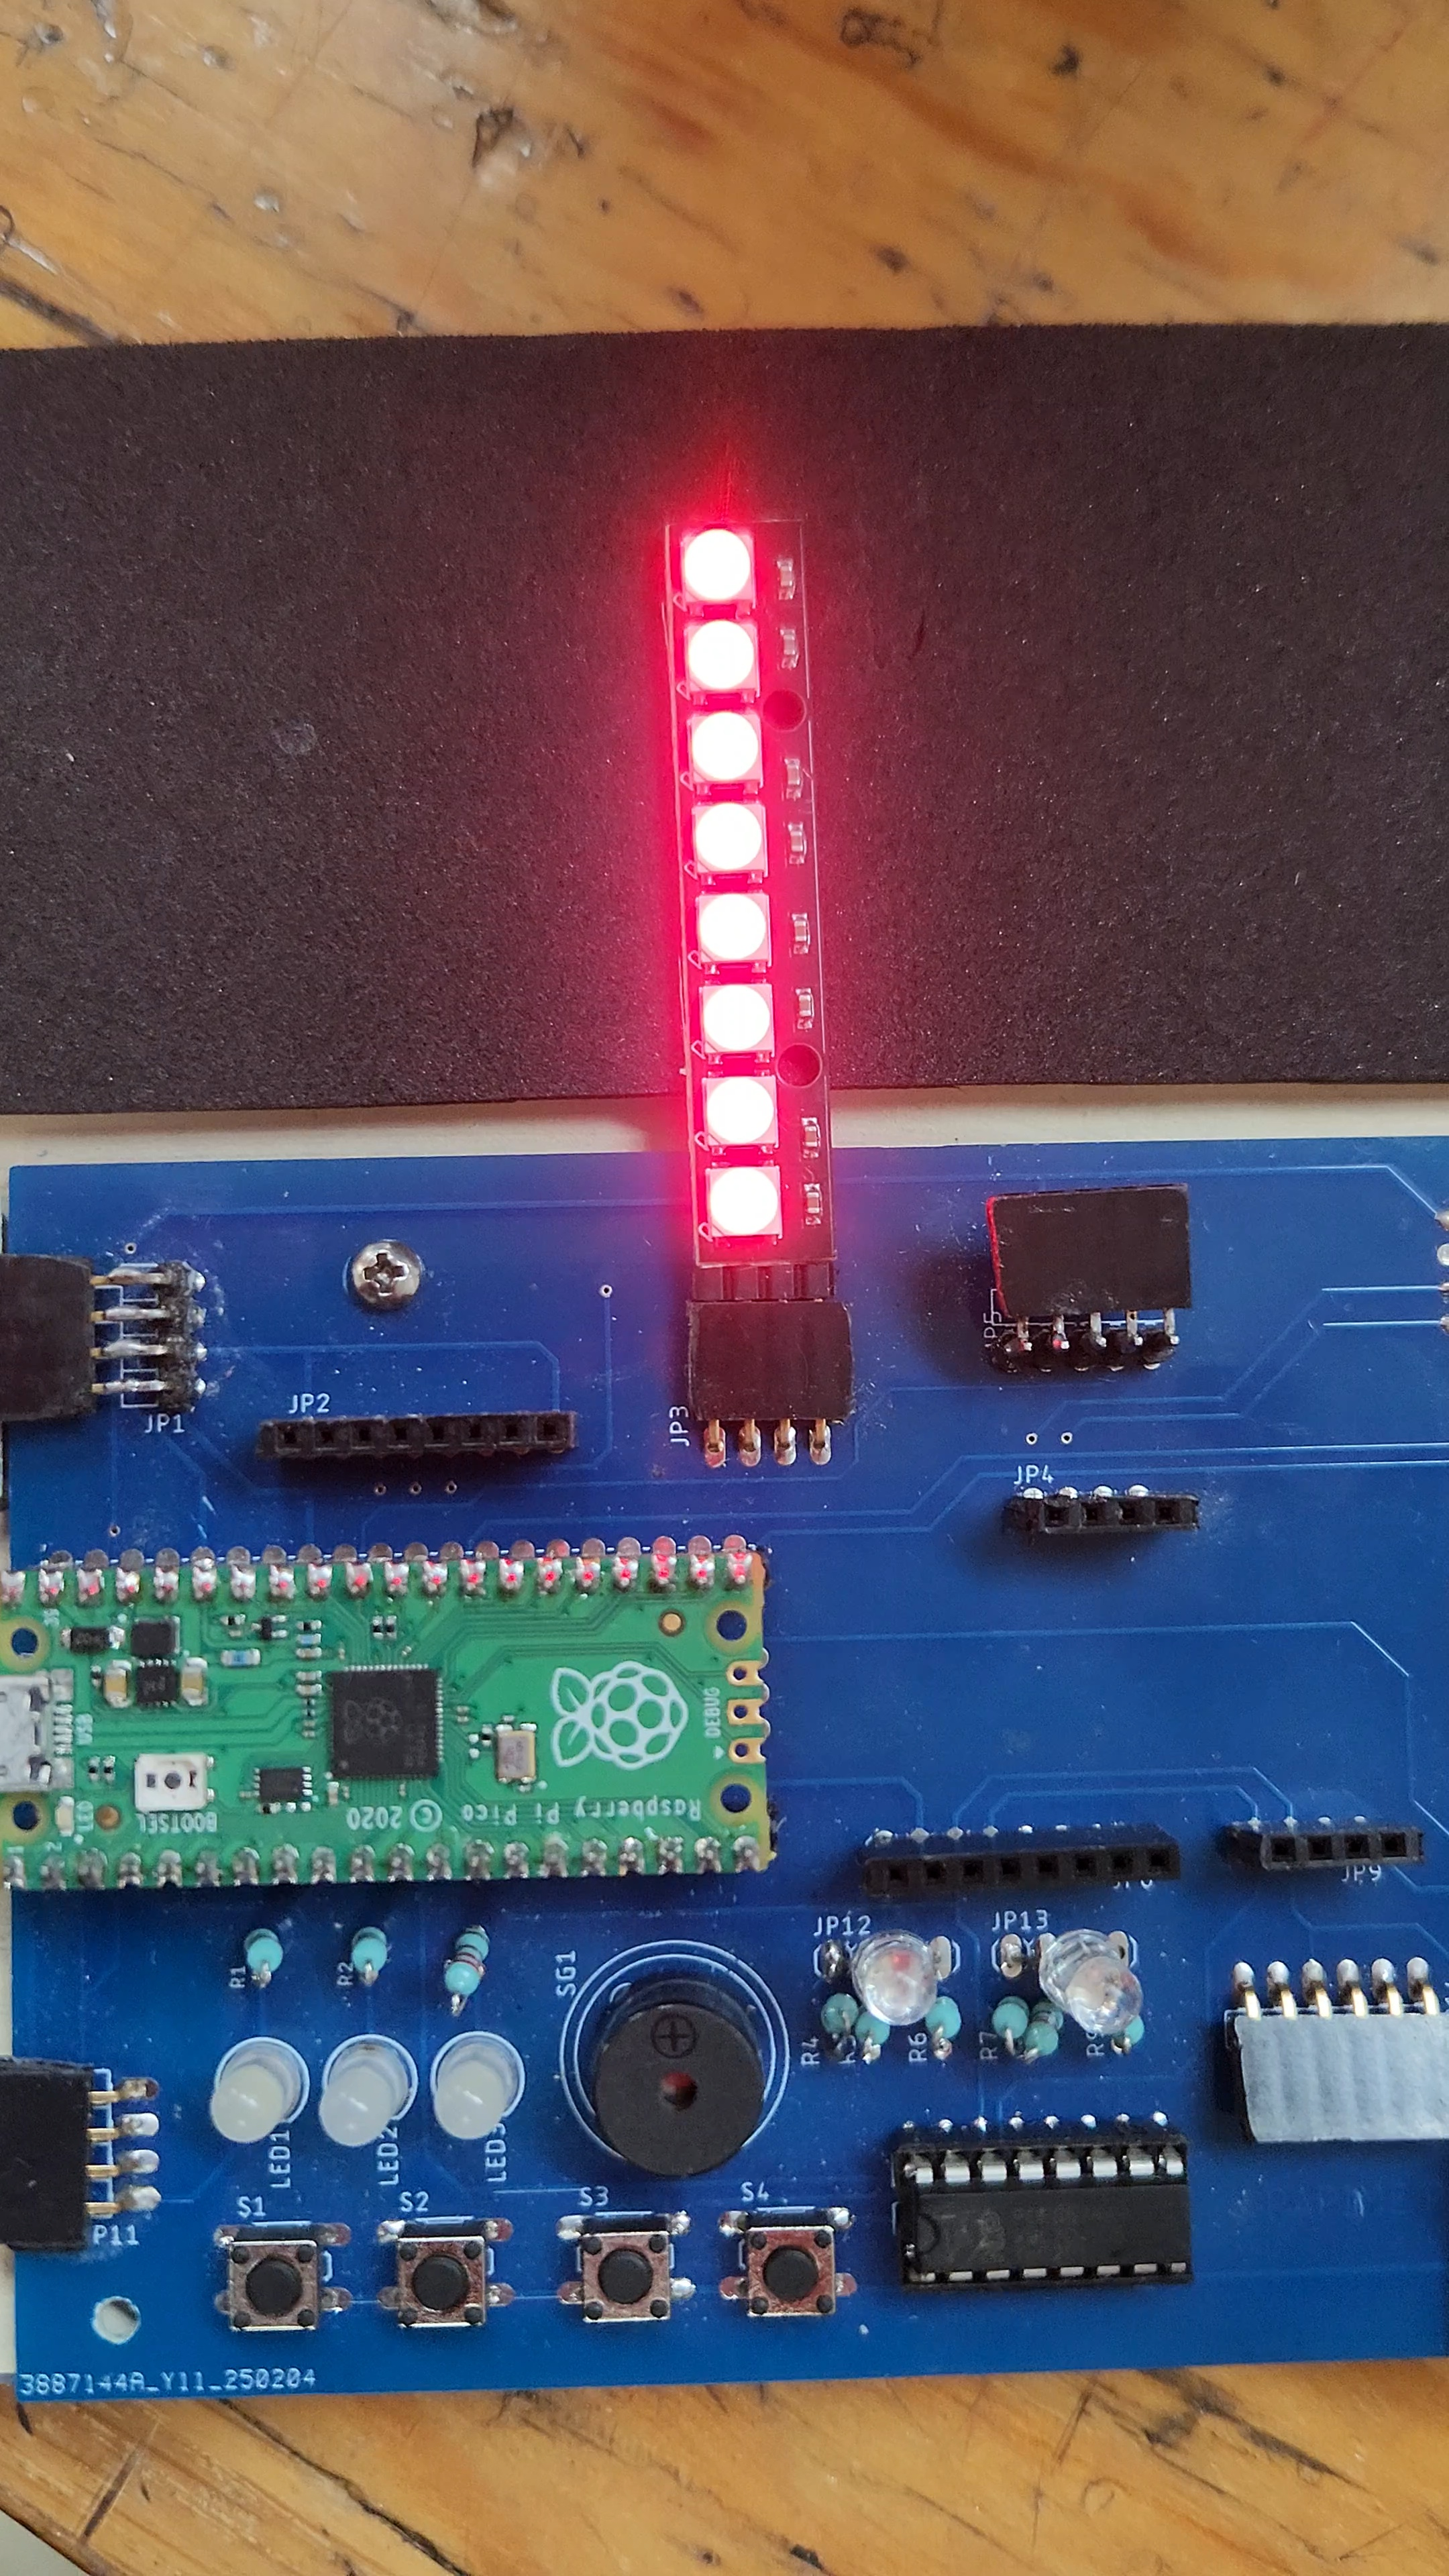
\includegraphics[width=\textwidth]{img/Actividad2/Act2_22.jpg}
        \caption{Posicion 8}
    \end{minipage}\hfill
    \begin{minipage}{0.3\textwidth}
        \centering
        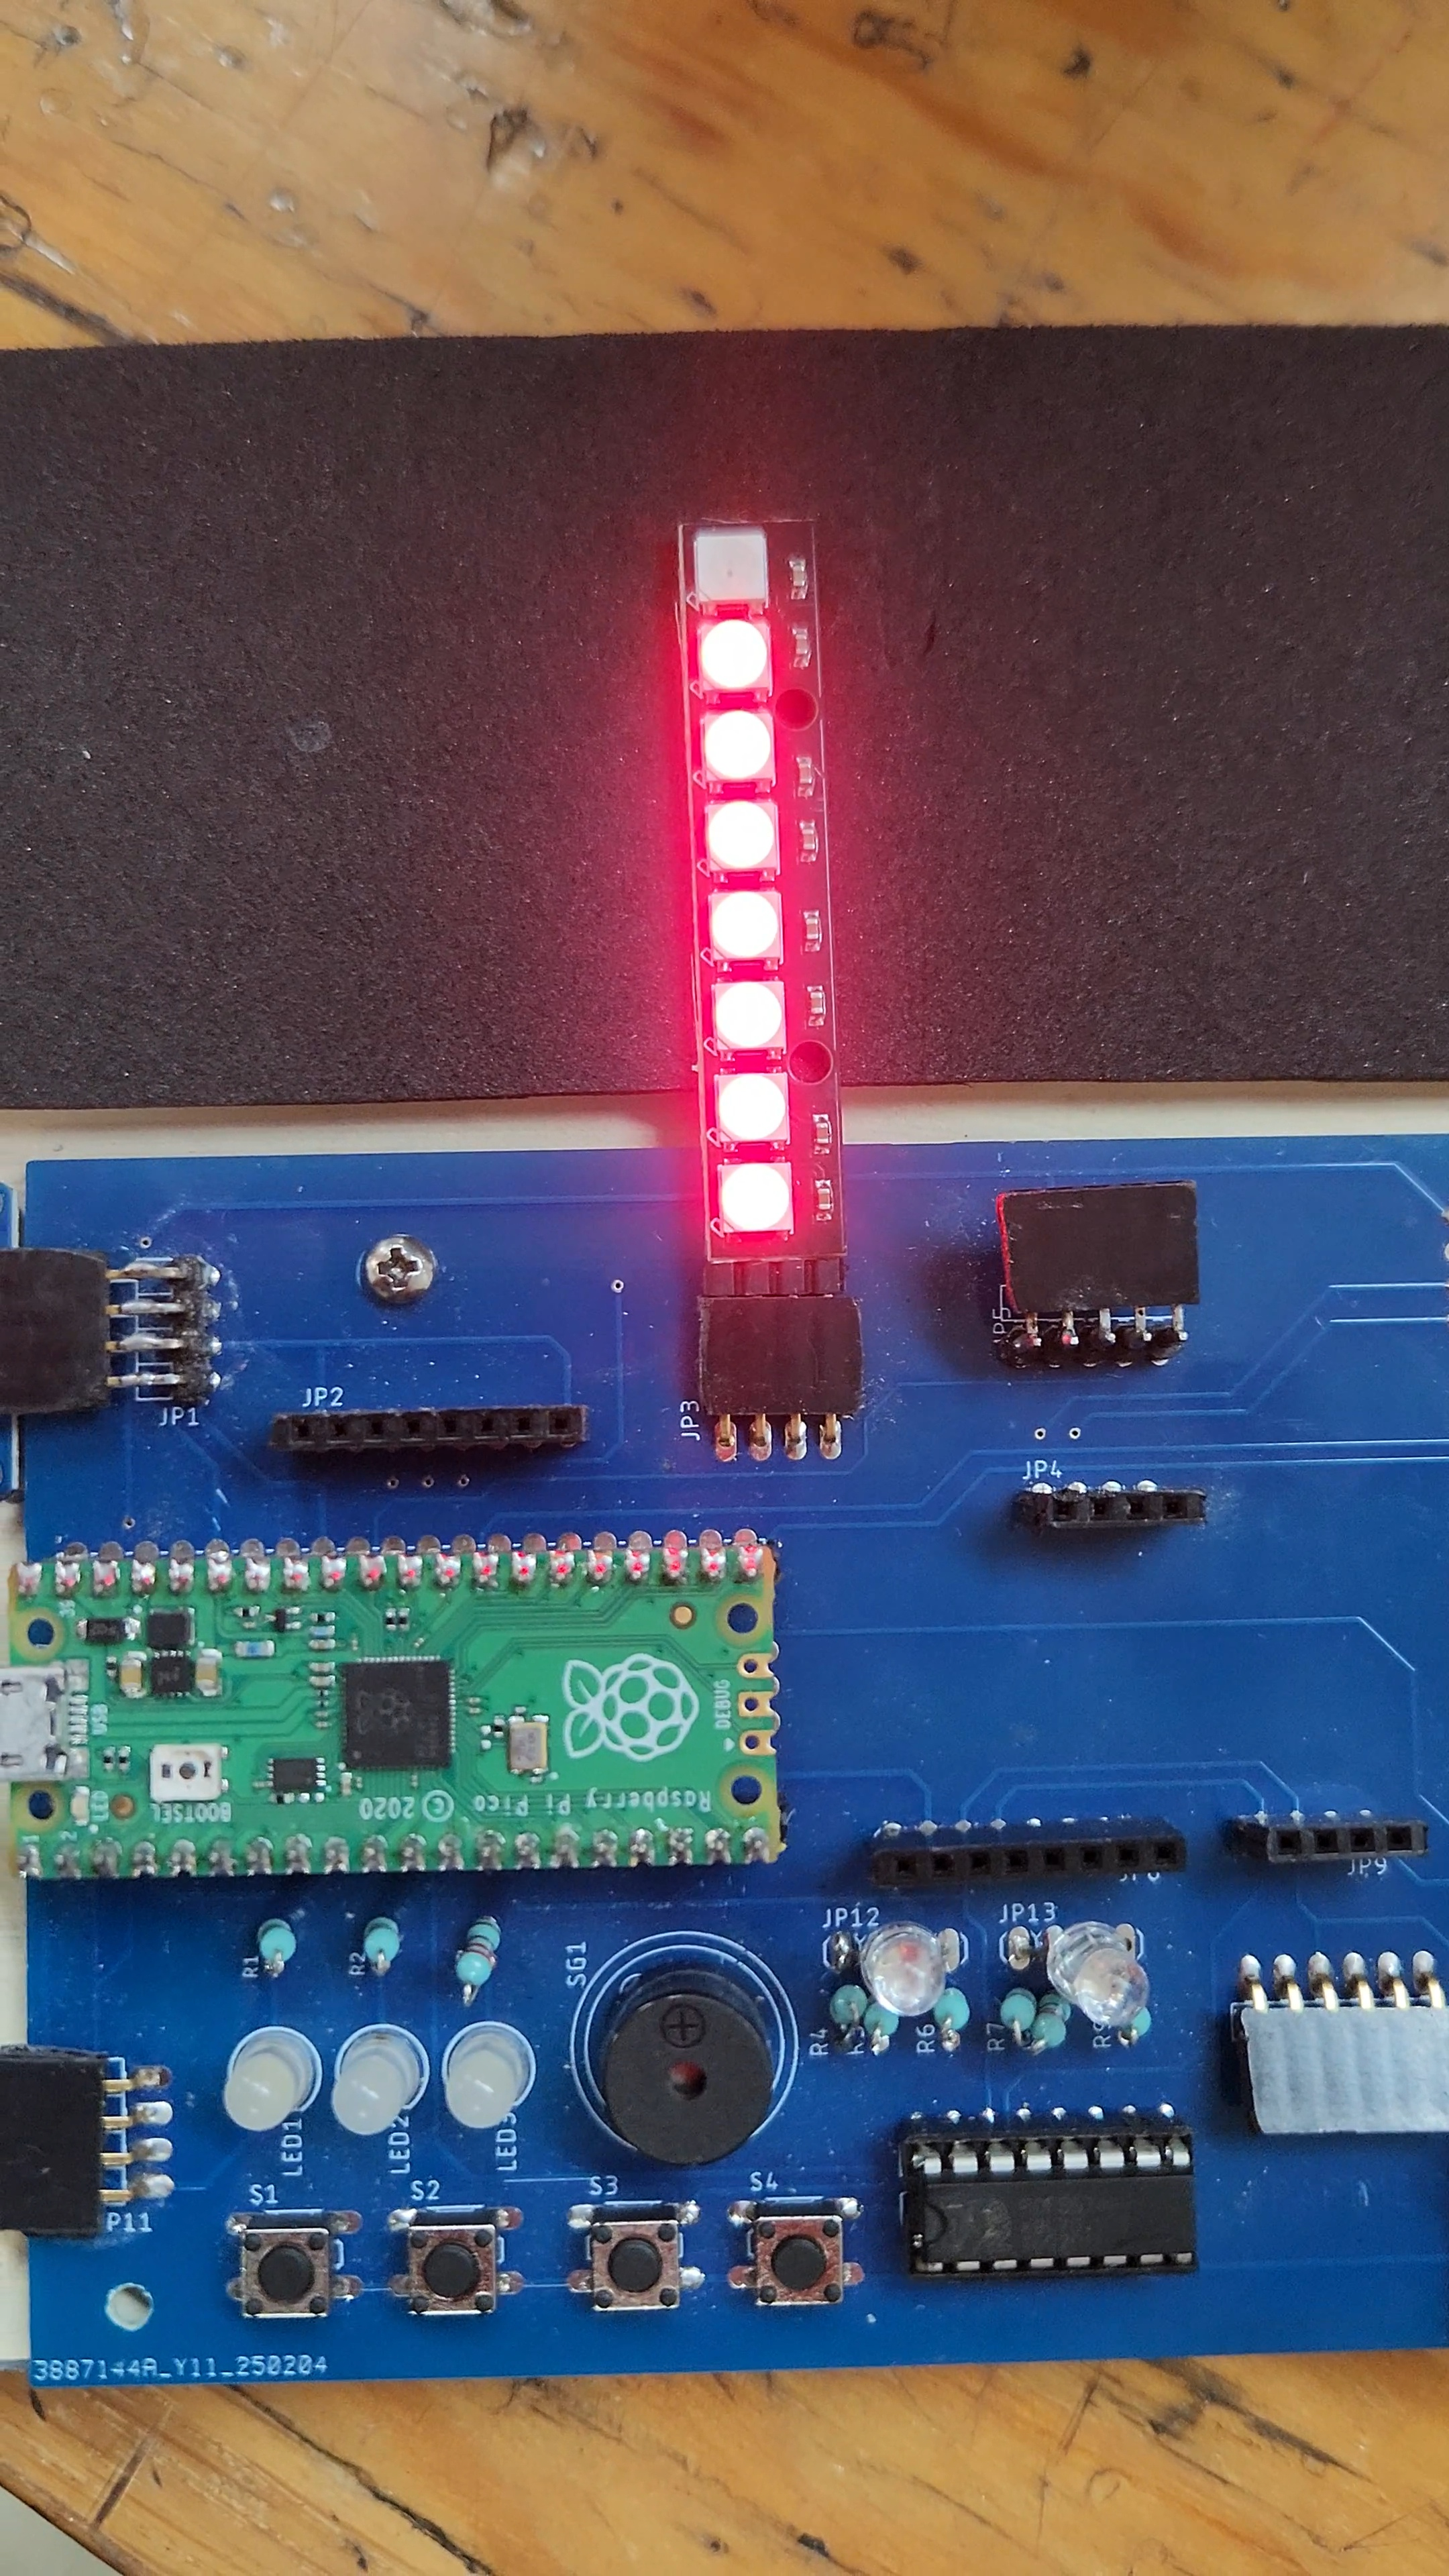
\includegraphics[width=\textwidth]{img/Actividad2/Act2_23.jpg}
        \caption{Posicion 9}
    \end{minipage}
\end{figure}

\begin{figure}[H]
    \centering
    \begin{minipage}{0.3\textwidth}
        \centering
        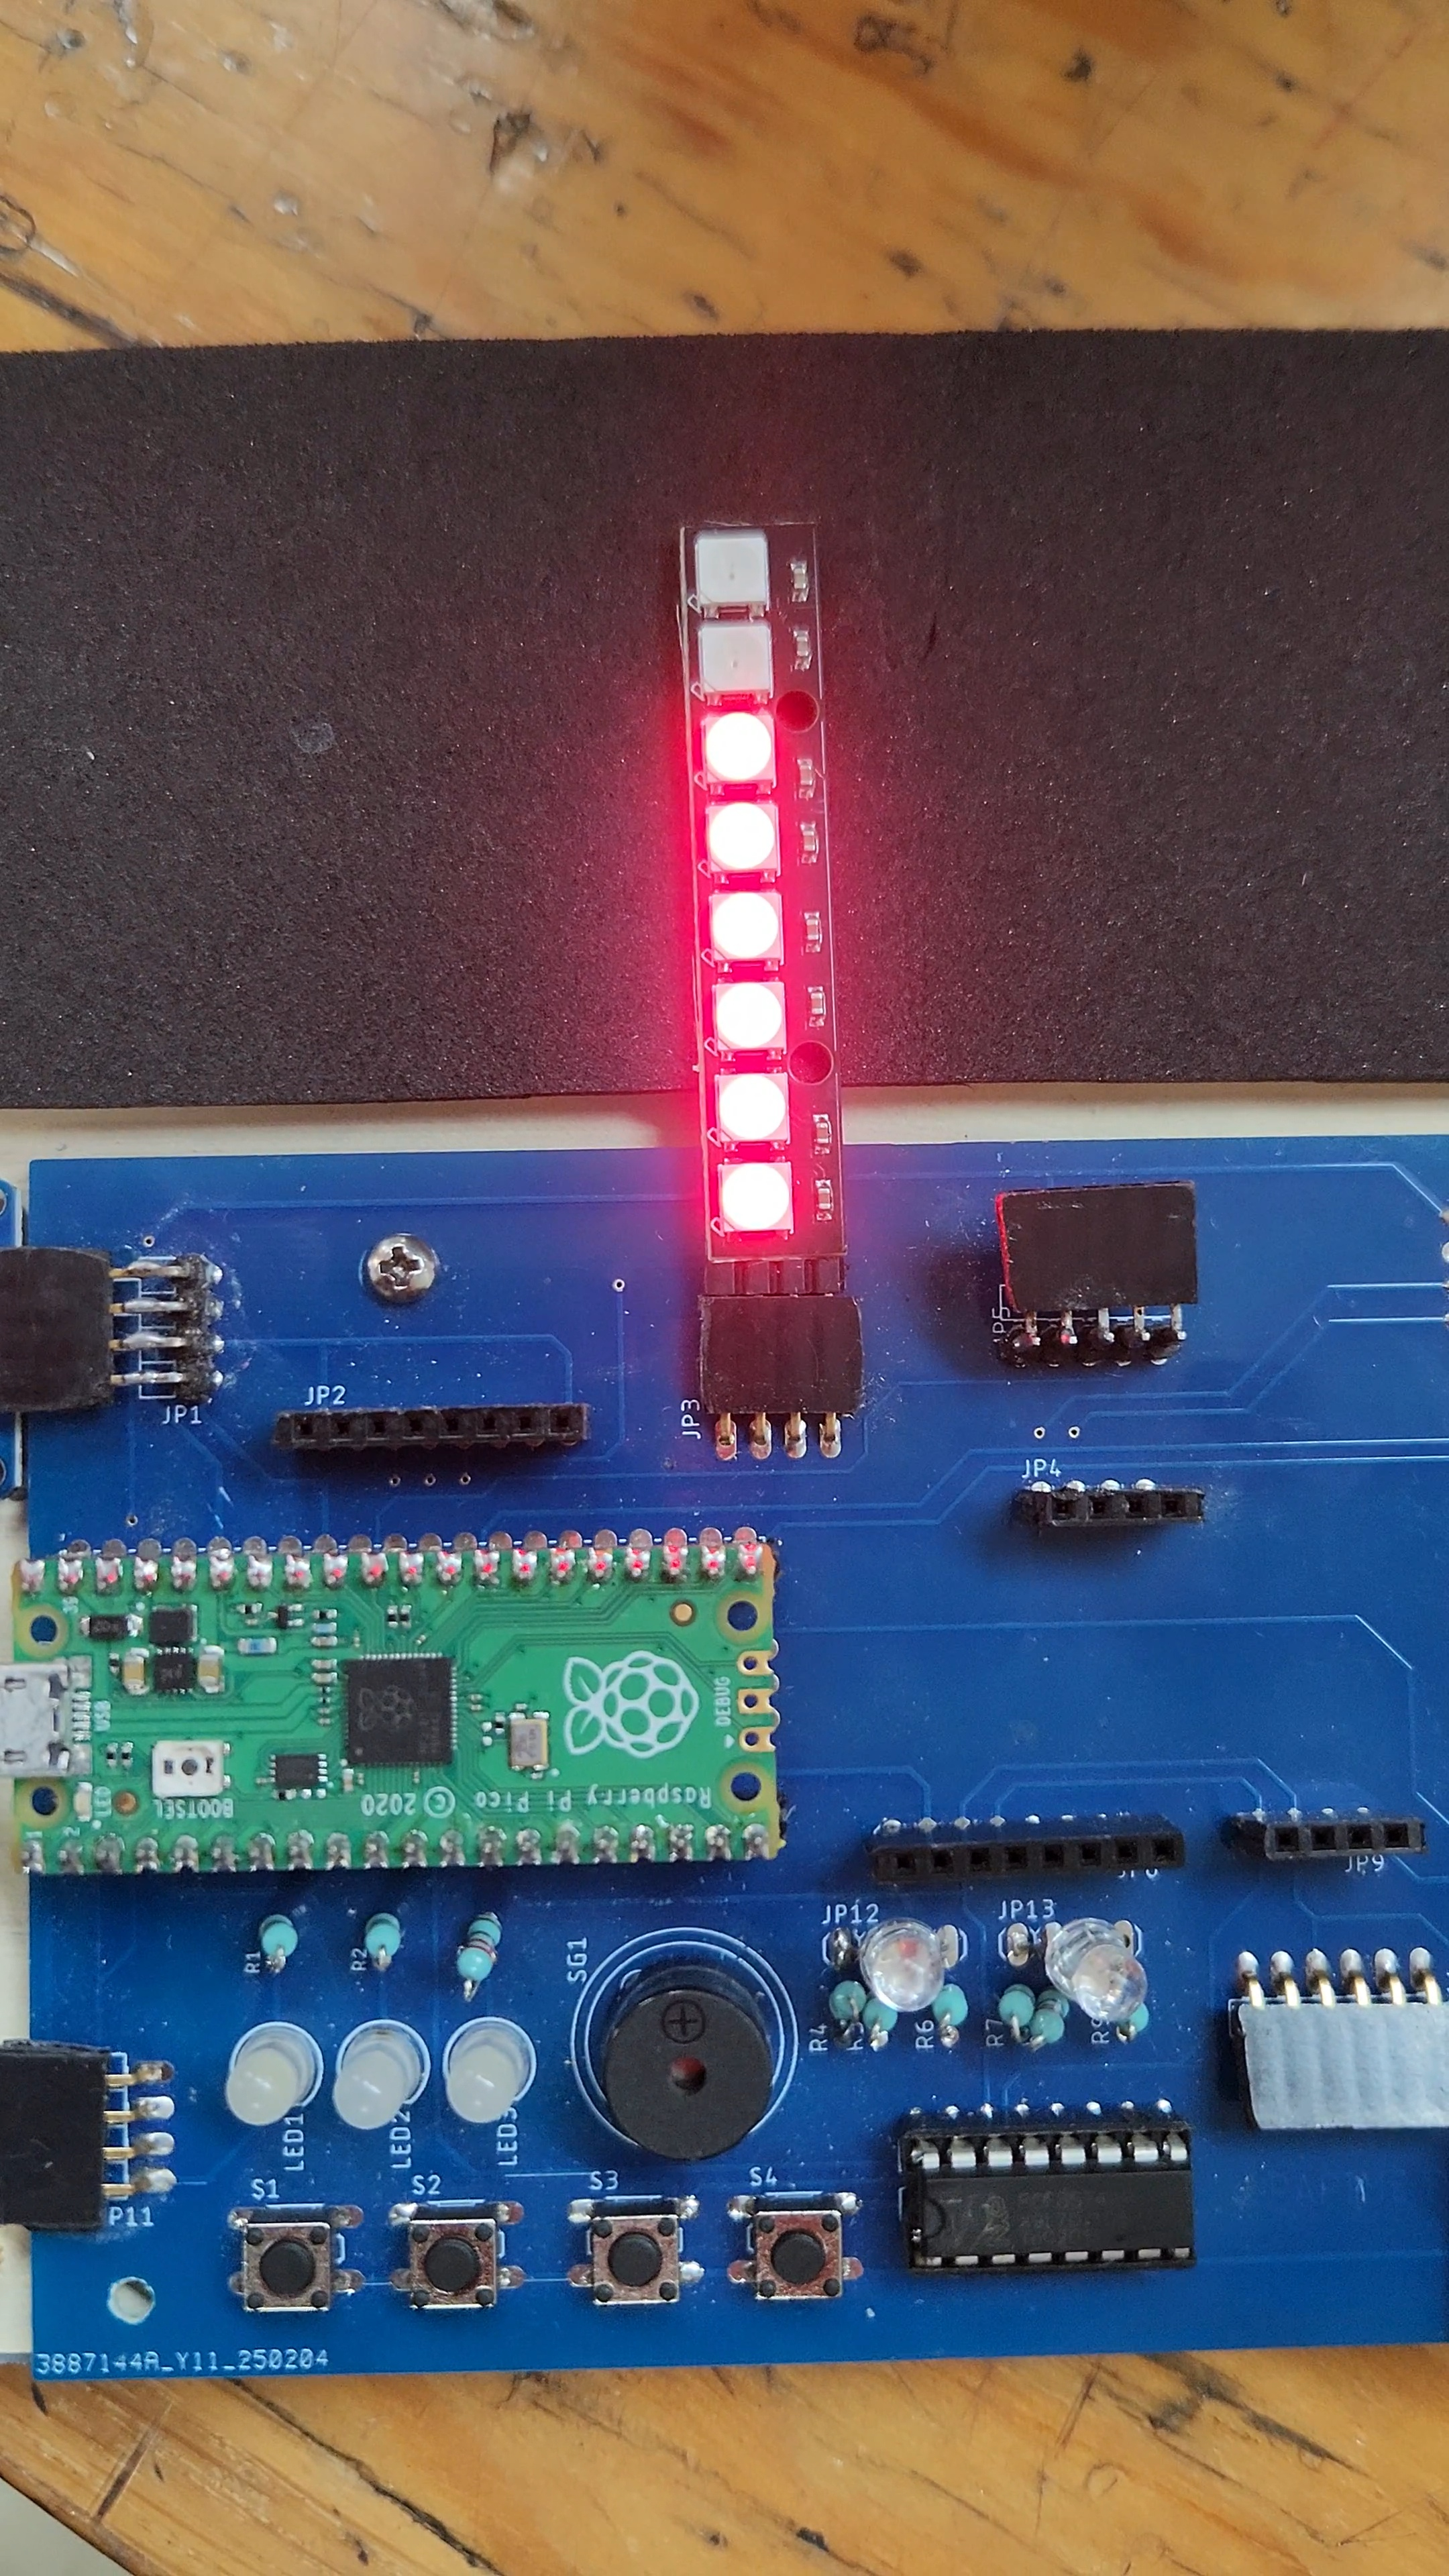
\includegraphics[width=\textwidth]{img/Actividad2/Act2_24.jpg}
        \caption{Posicion 10}
    \end{minipage}\hfill
    \begin{minipage}{0.3\textwidth}
        \centering
        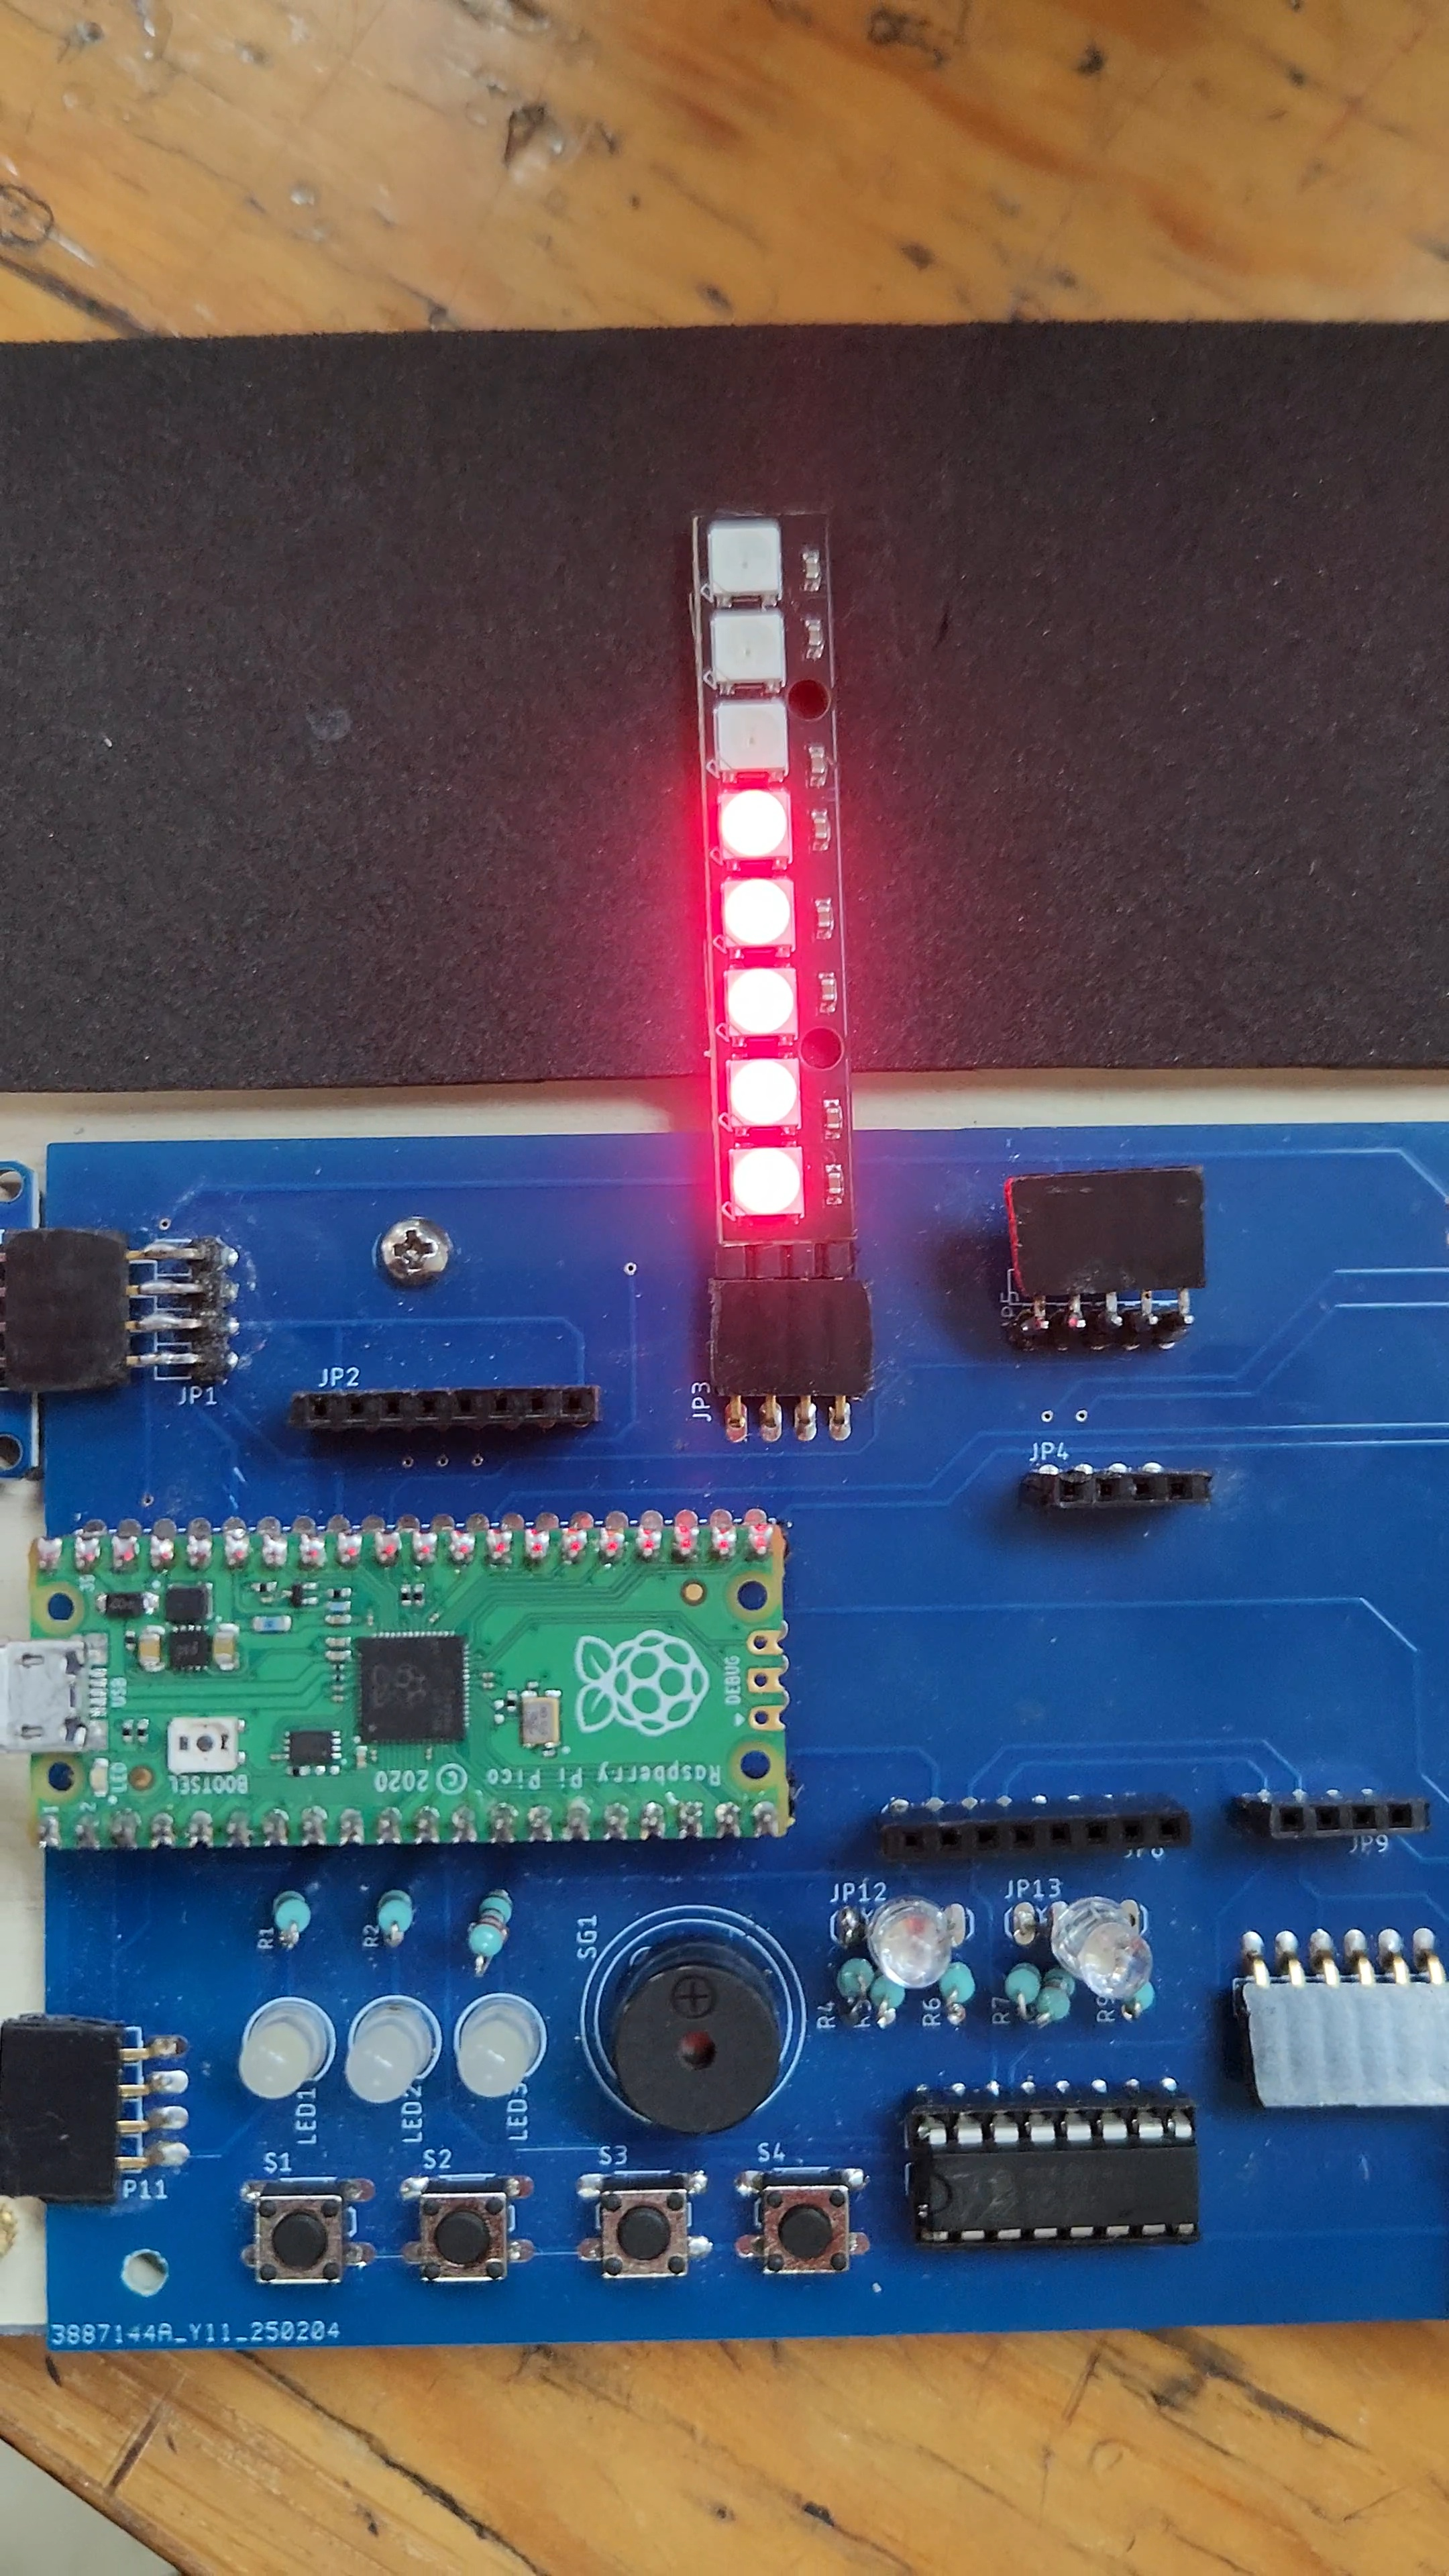
\includegraphics[width=\textwidth]{img/Actividad2/Act2_25.jpg}
        \caption{Posicion 11}
    \end{minipage}\hfill
    \begin{minipage}{0.3\textwidth}
        \centering
        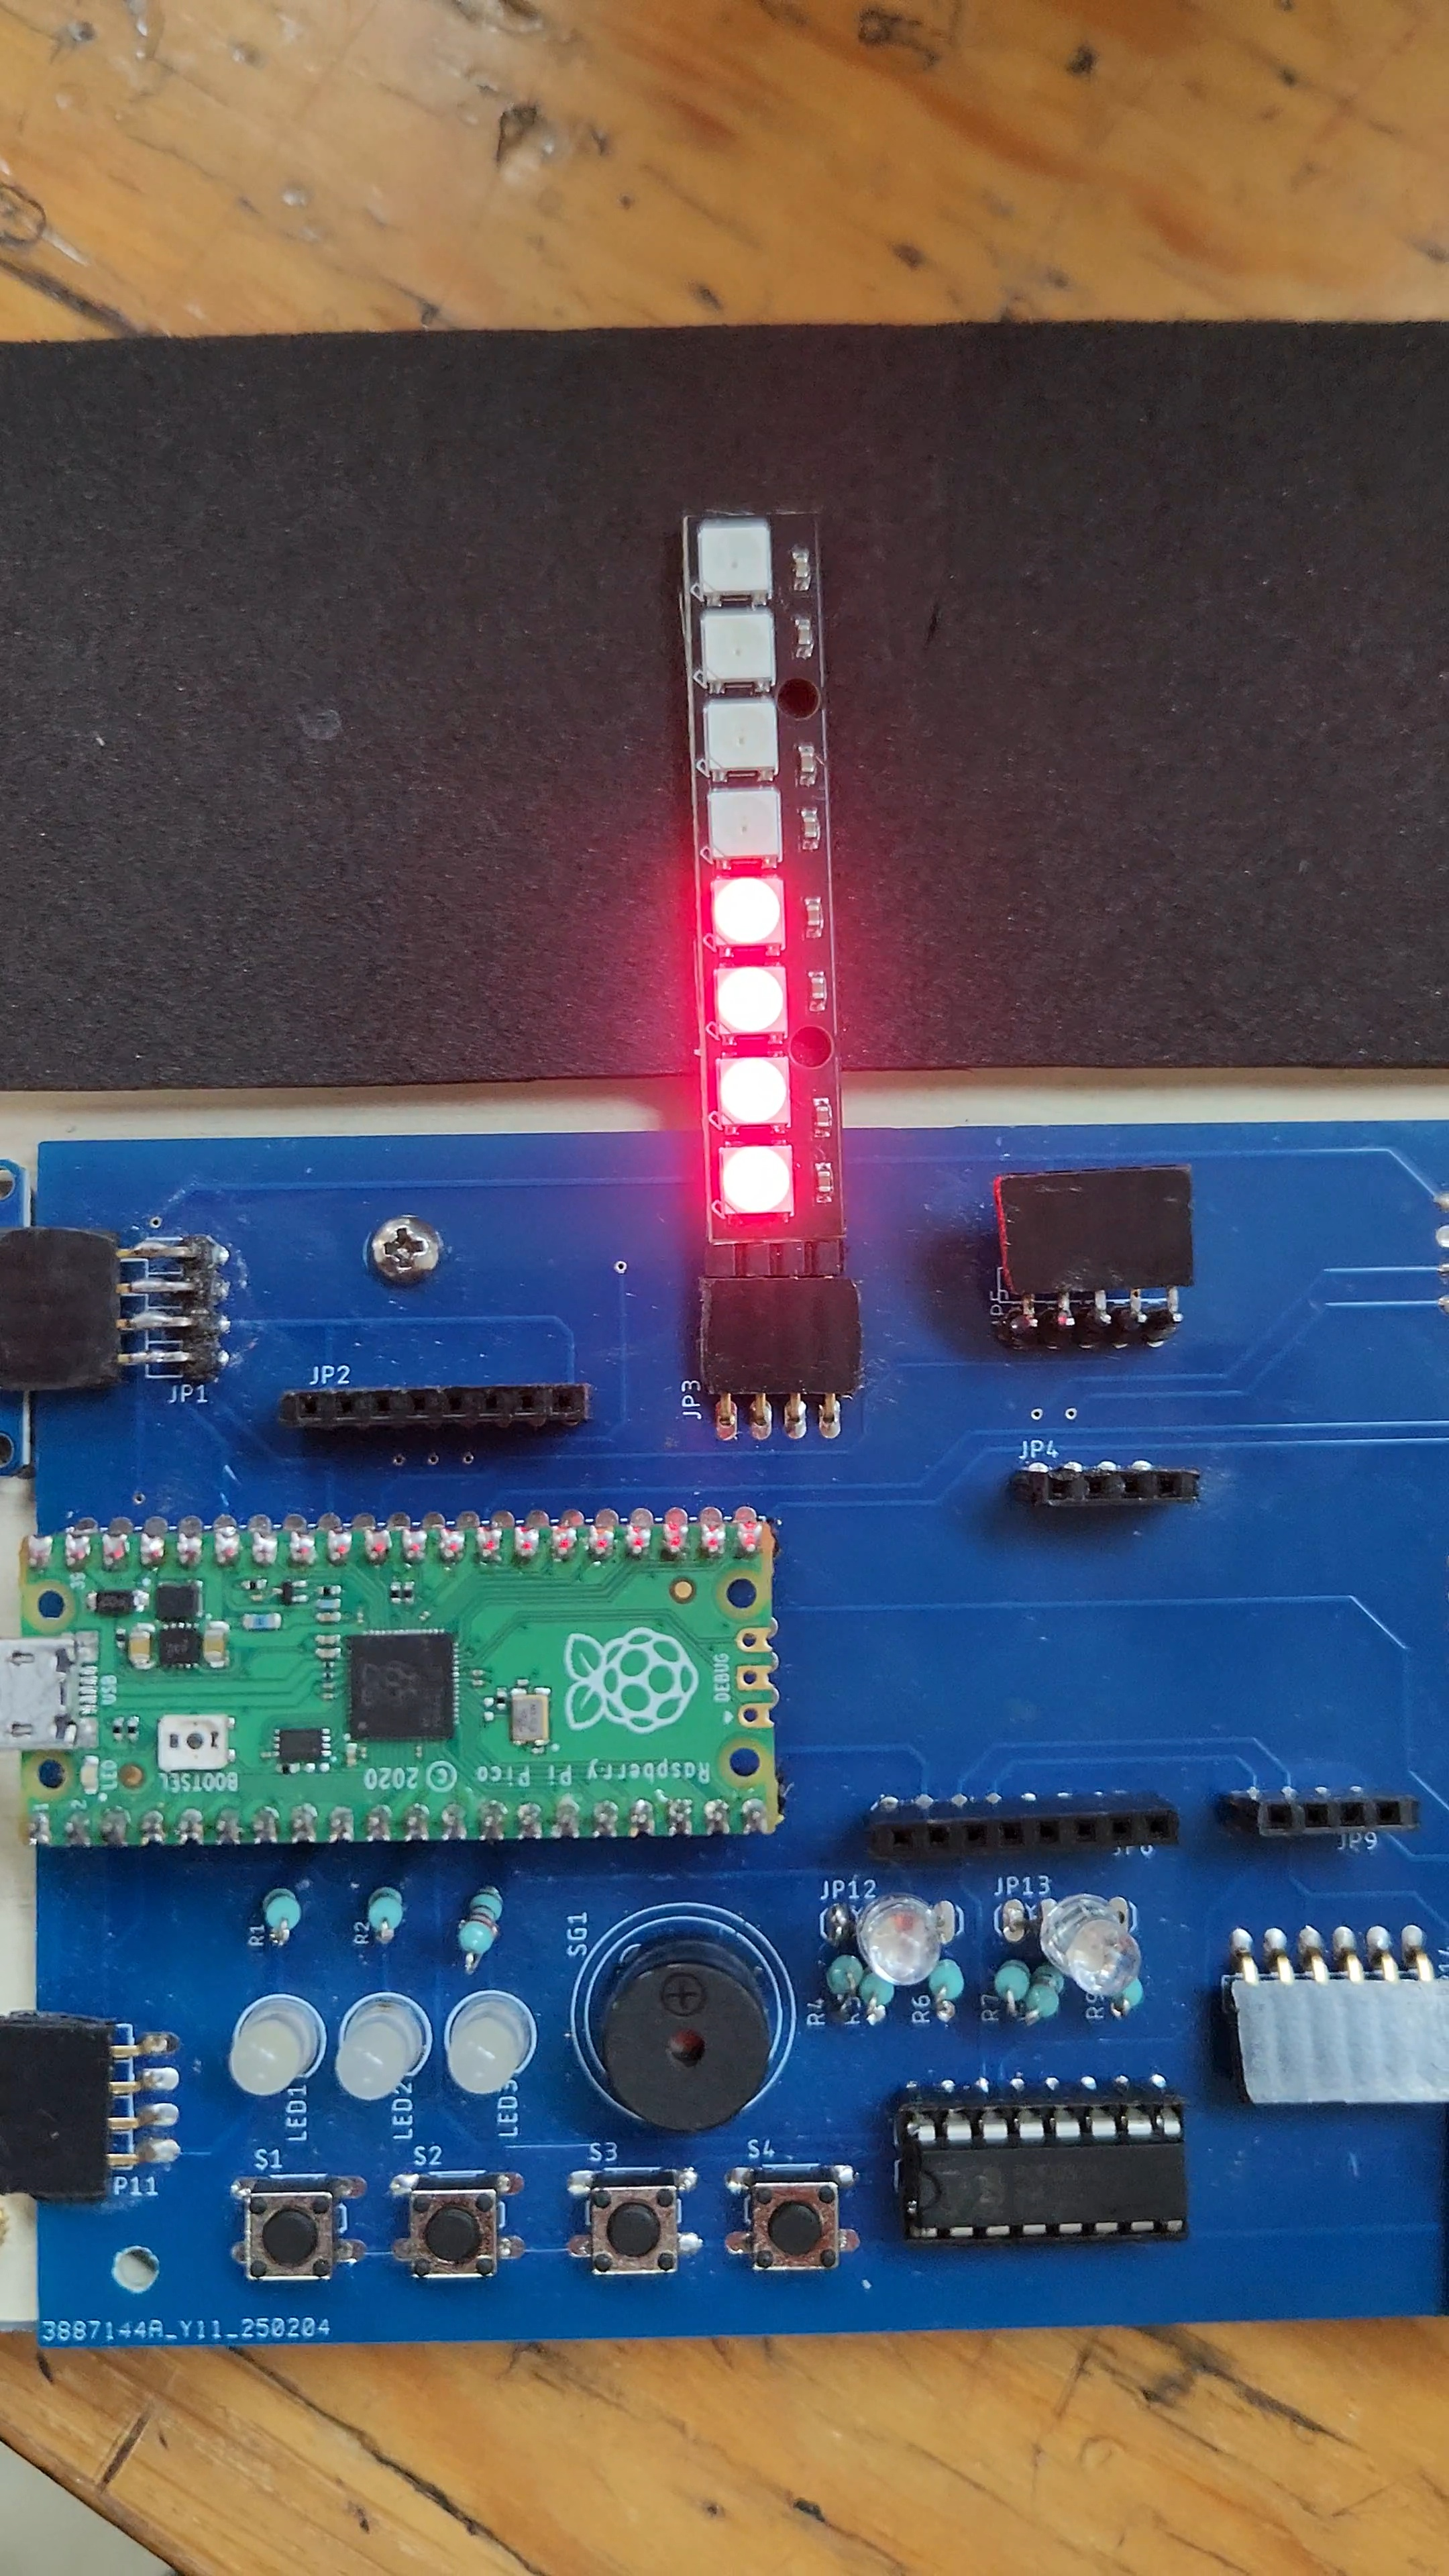
\includegraphics[width=\textwidth]{img/Actividad2/Act2_26.jpg}
        \caption{Posicion 12}
    \end{minipage}
\end{figure}

\begin{figure}[H]
    \centering
    \begin{minipage}{0.3\textwidth}
        \centering
        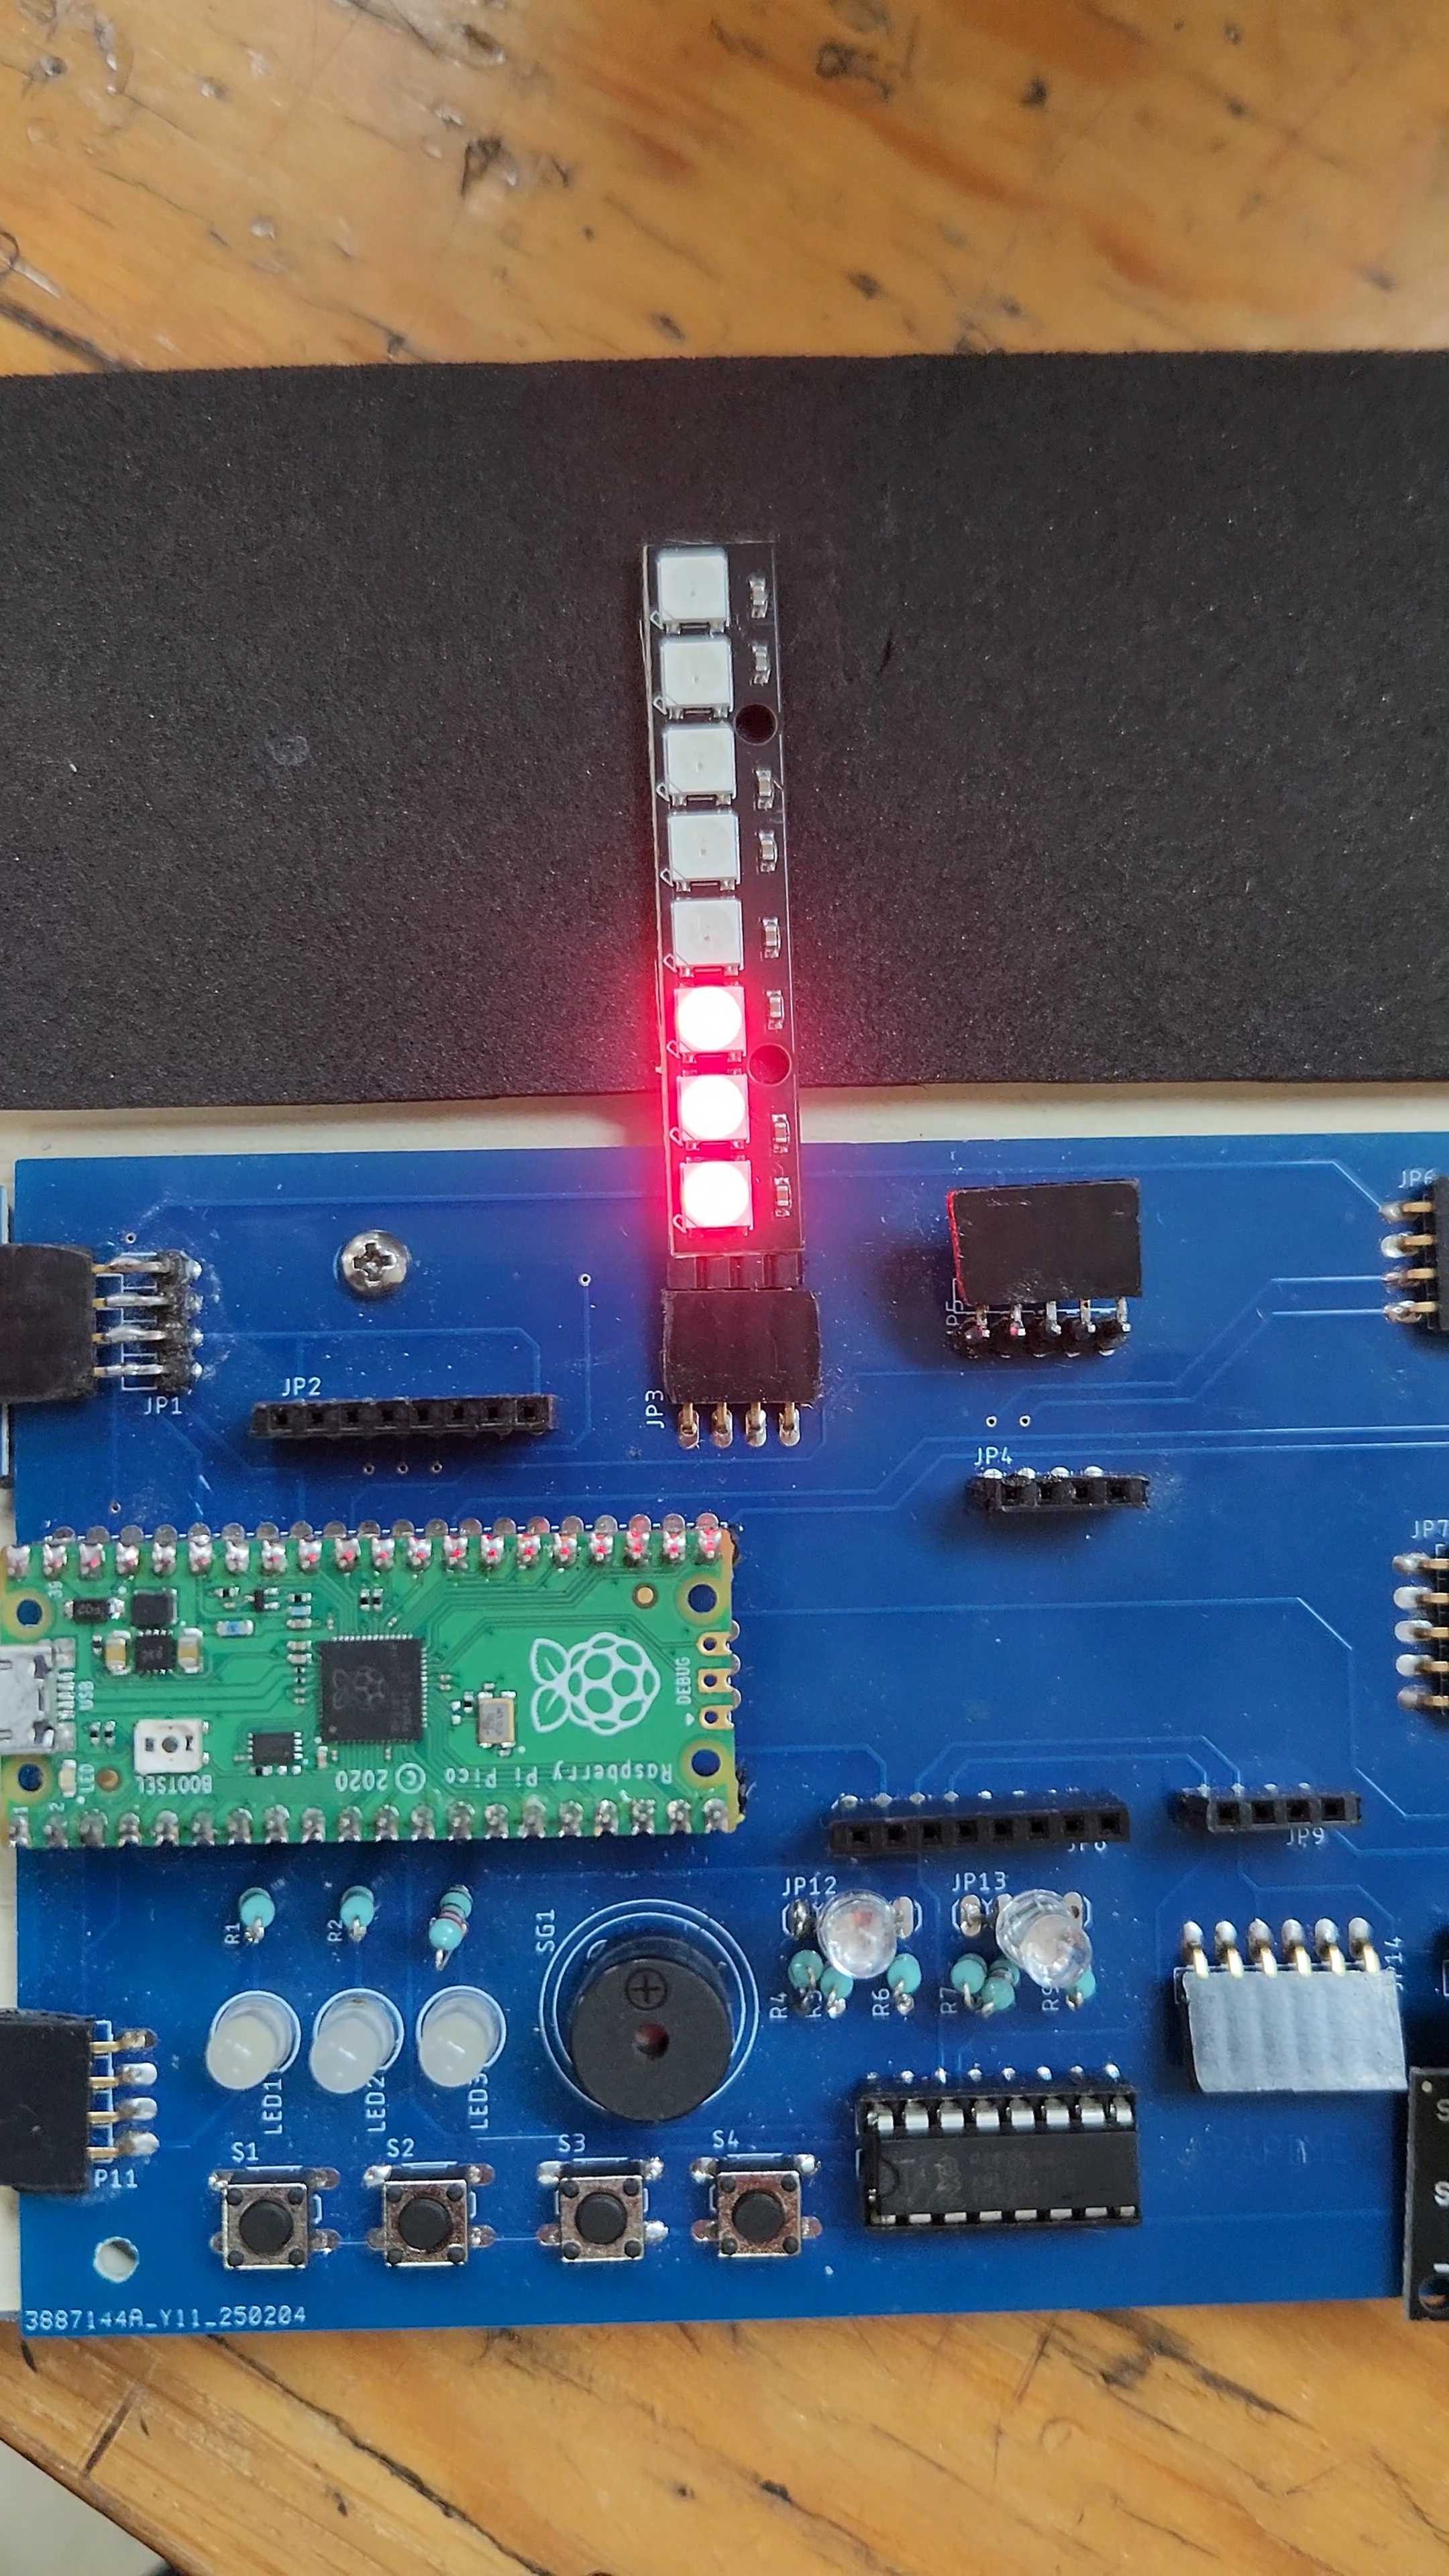
\includegraphics[width=\textwidth]{img/Actividad2/Act2_27.jpg}
        \caption{Posicion 13}
    \end{minipage}\hfill
    \begin{minipage}{0.3\textwidth}
        \centering
        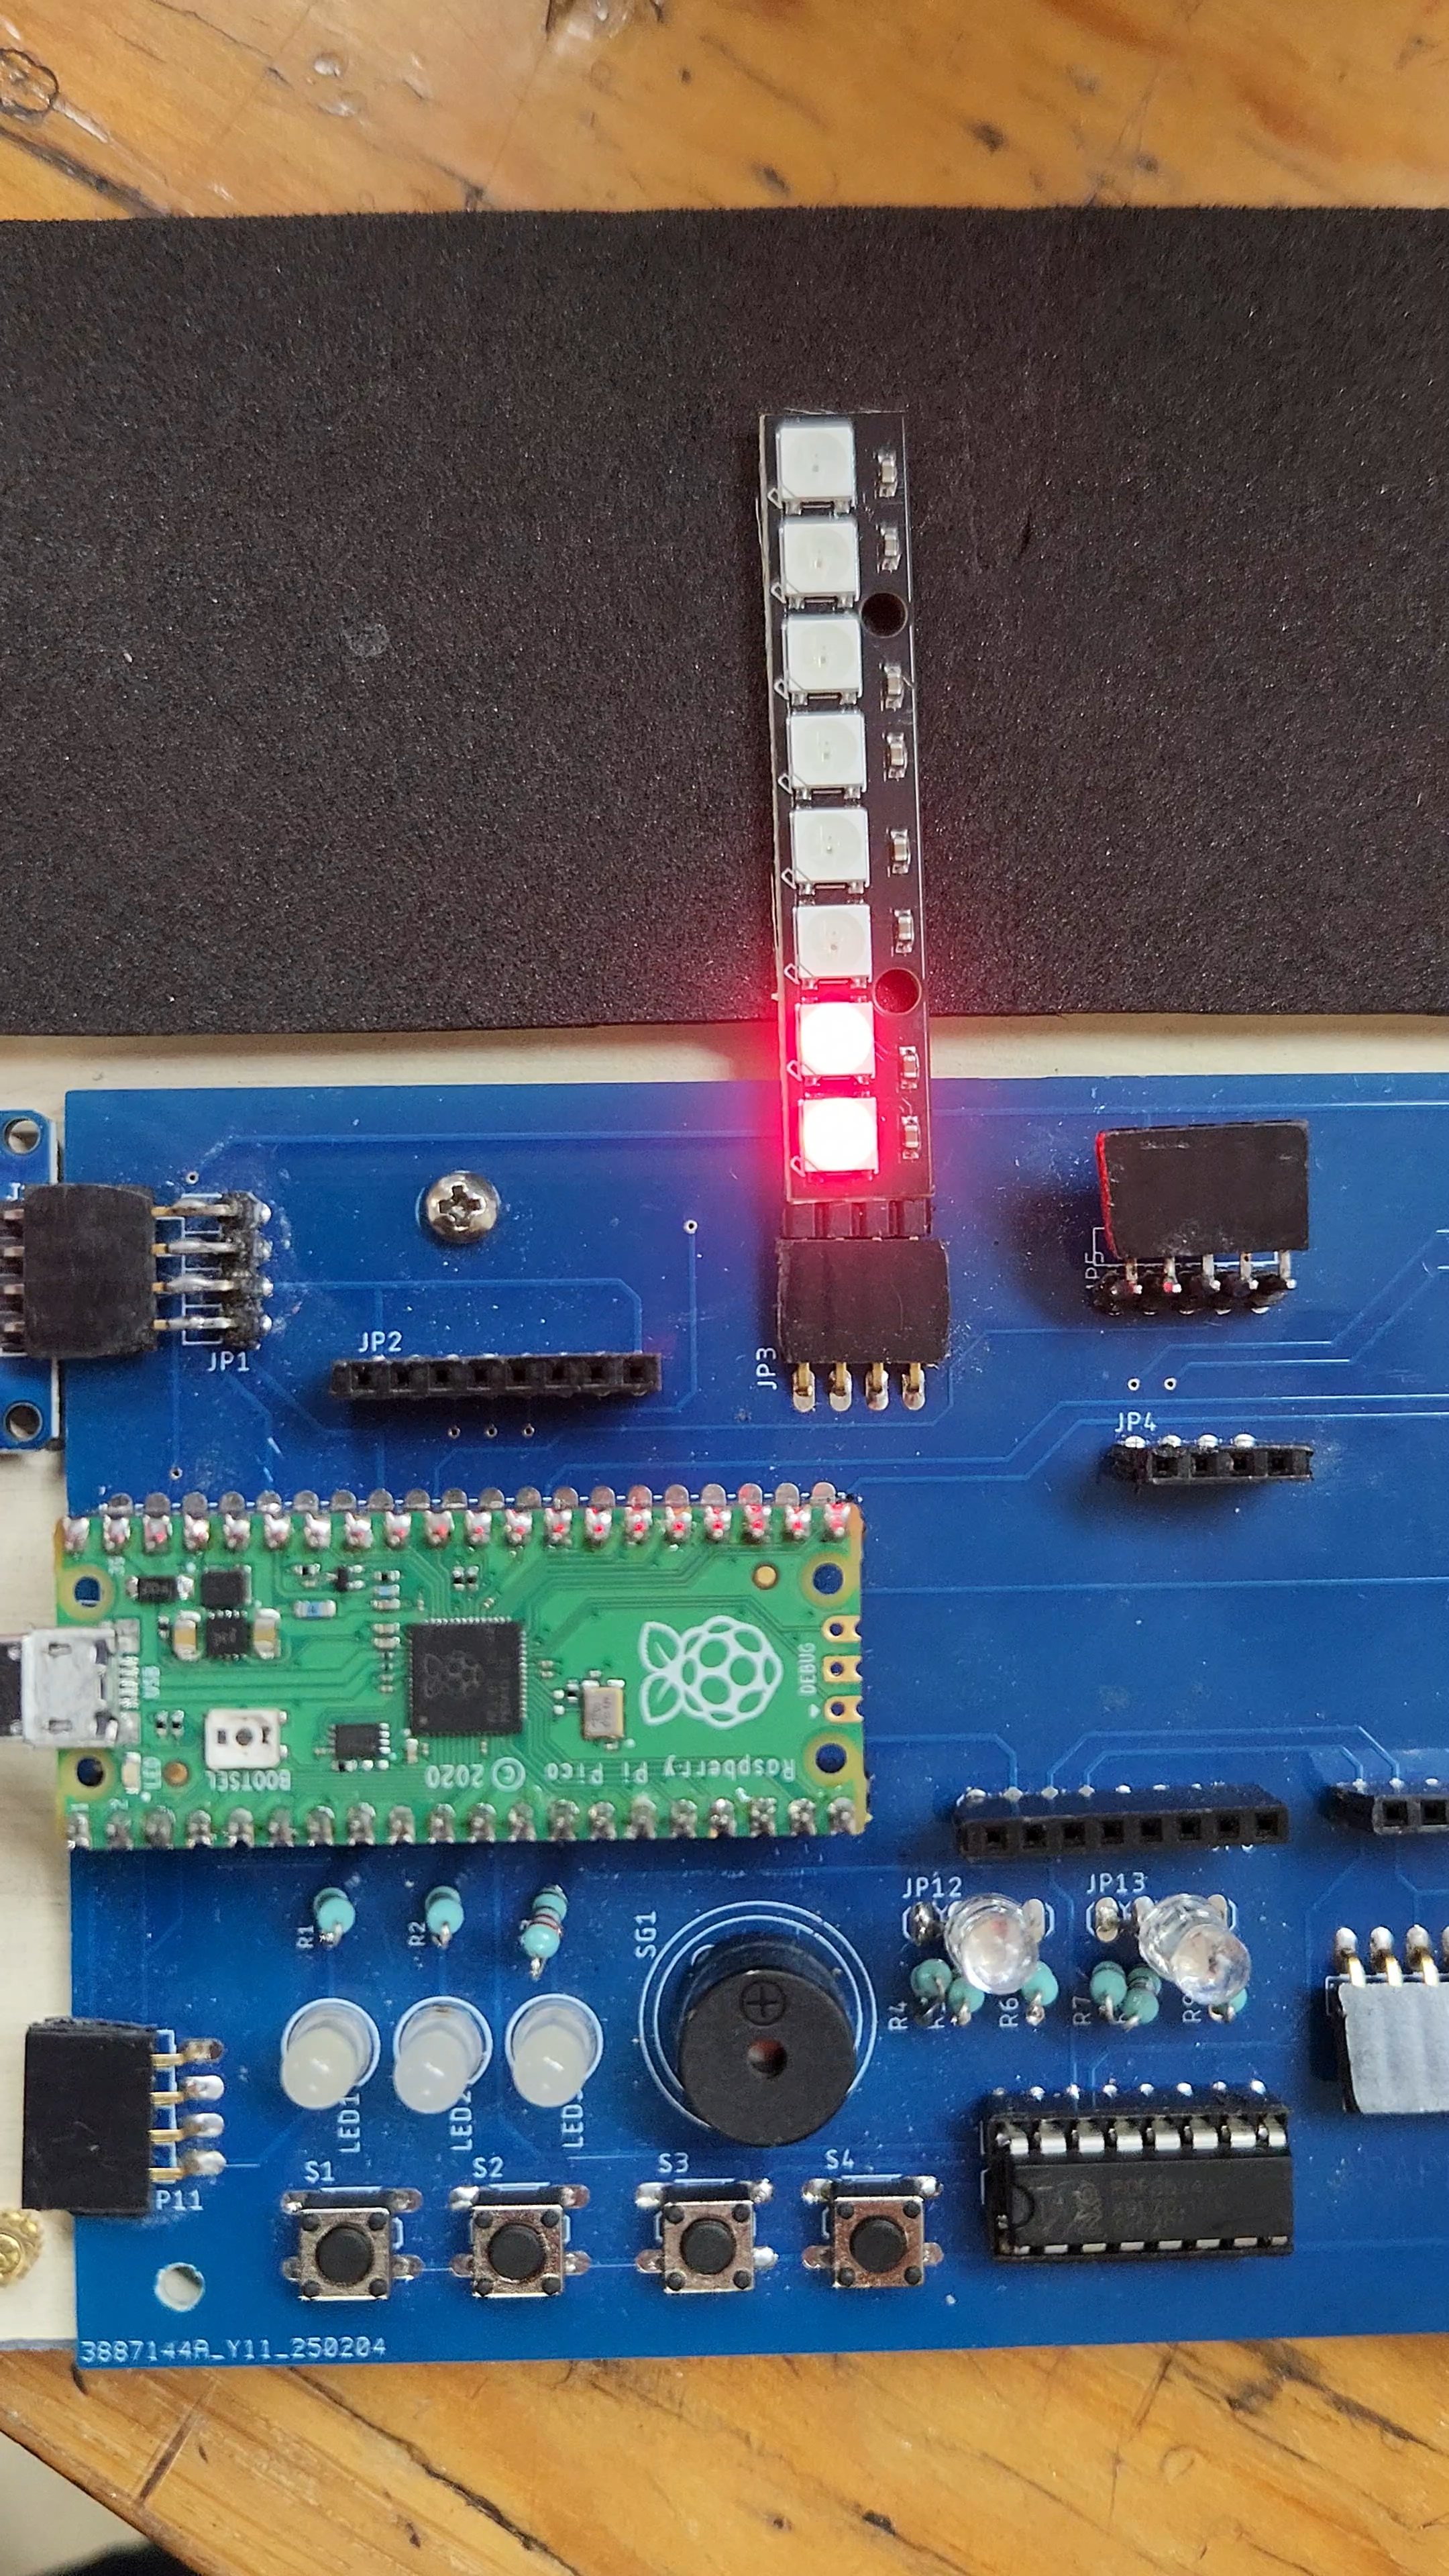
\includegraphics[width=\textwidth]{img/Actividad2/Act2_20.jpg}
        \caption{Posicion 14}
    \end{minipage}\hfill
    \begin{minipage}{0.3\textwidth}
        \centering
        
\includegraphics[width=\textwidth]{img/Actividad2/Act2_2.jpg}
        \caption{Posicion 15}
    \end{minipage}
\end{figure}

% ==========================================
% BLOQUE 2: Color Verde (15 imagenes)
% ==========================================
\textbf{Secuencia en color verde}

\begin{figure}[H]
    \centering
    \begin{minipage}{0.3\textwidth}
        \centering
        
\includegraphics[width=\textwidth]{img/Actividad2/Act2_3.jpg}
        \caption{Posicion 1}
    \end{minipage}\hfill
    \begin{minipage}{0.3\textwidth}
        \centering
        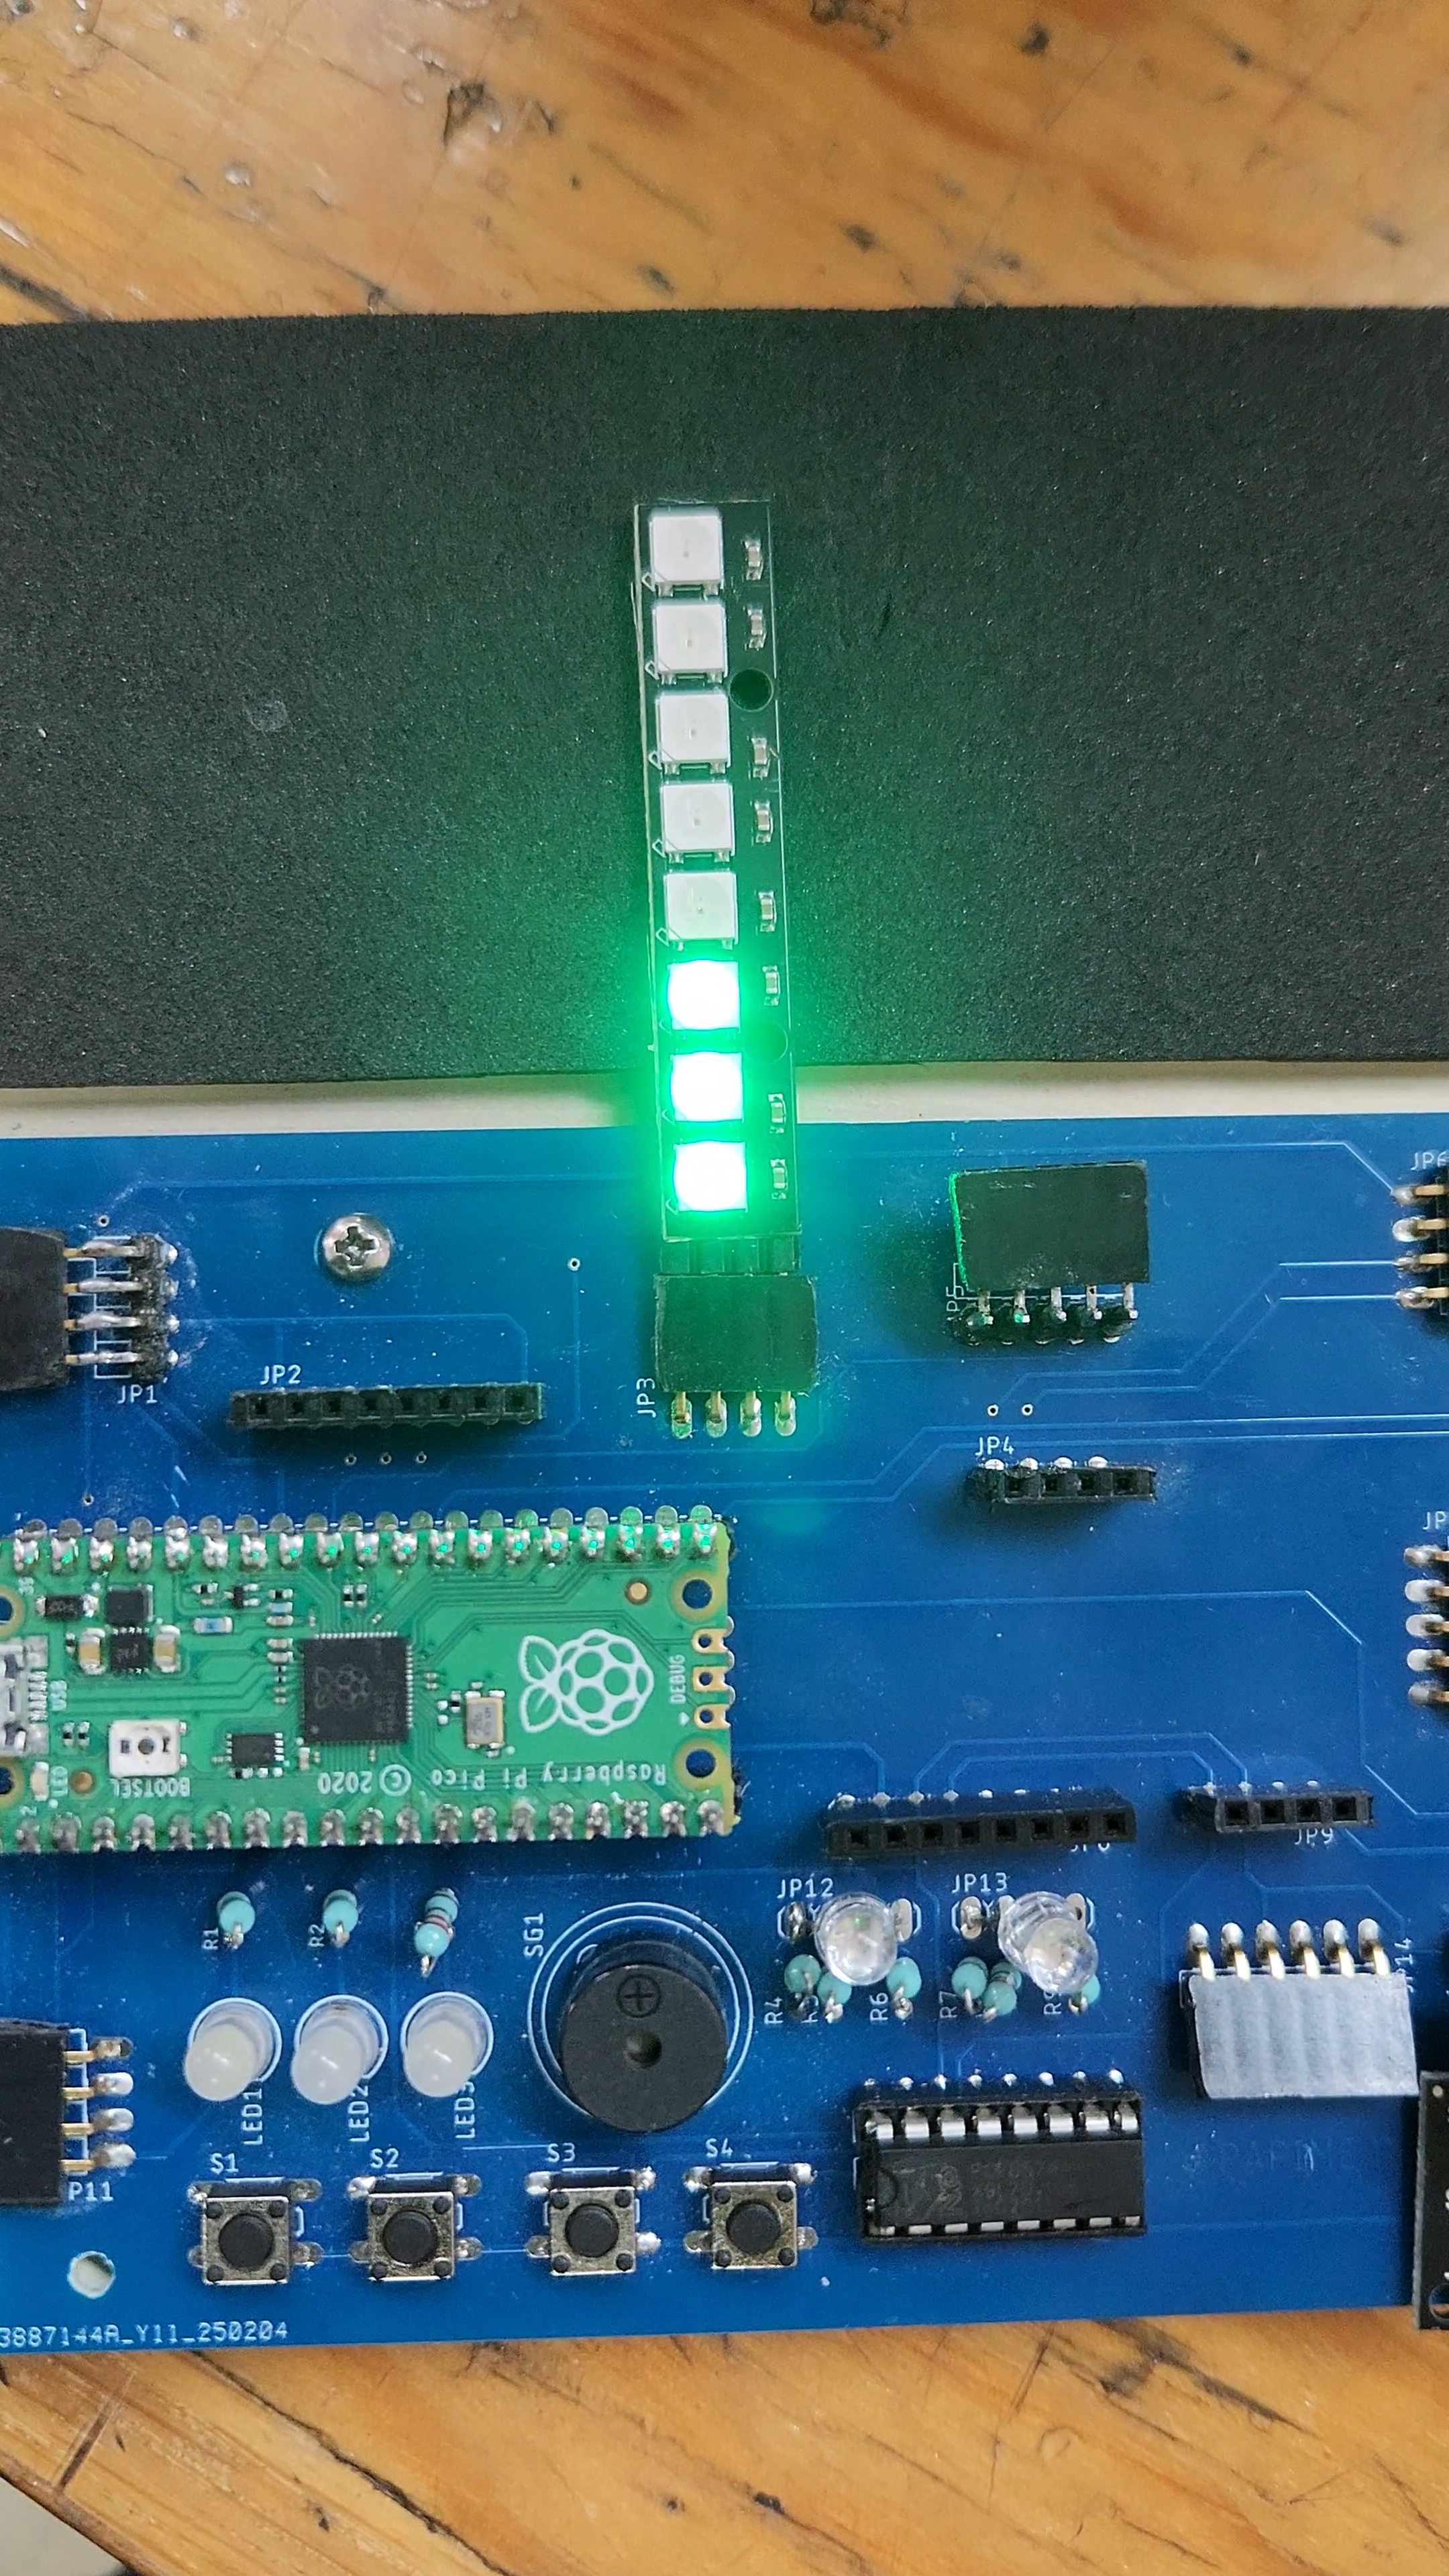
\includegraphics[width=\textwidth]{img/Actividad2/Act2_4.jpg}
        \caption{Posicion 3}
    \end{minipage}\hfill
    \begin{minipage}{0.3\textwidth}
        \centering
        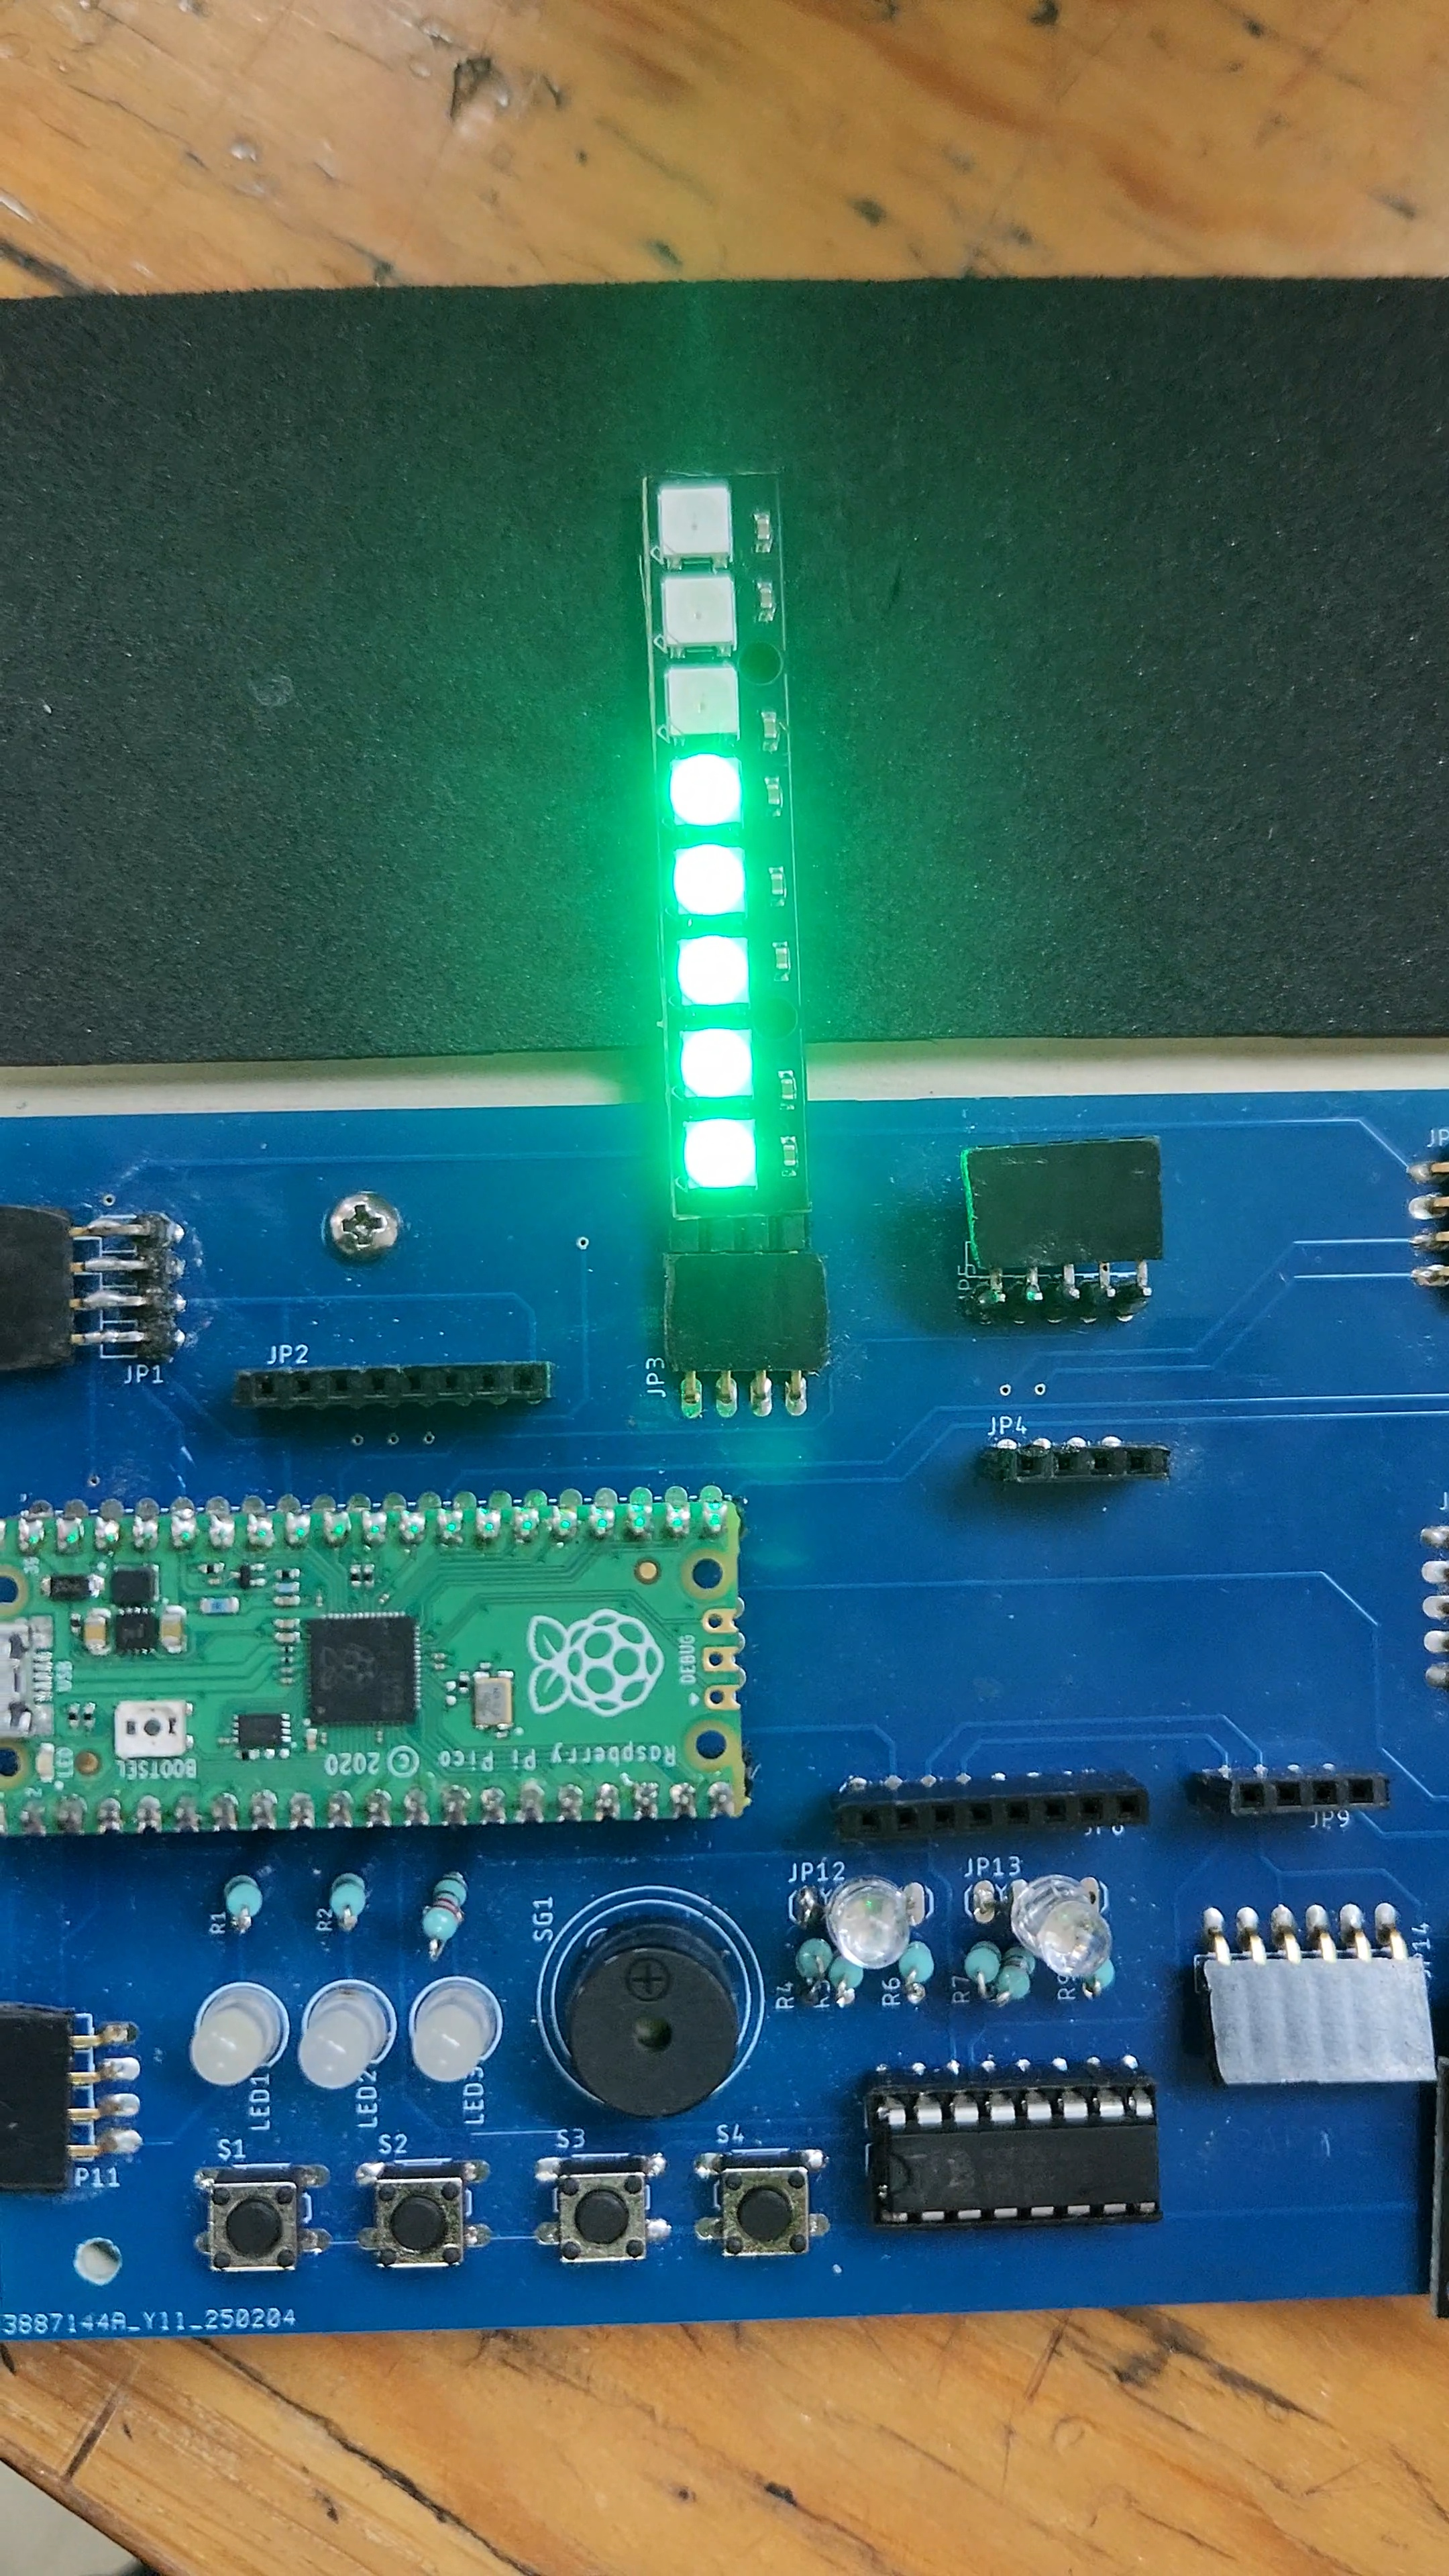
\includegraphics[width=\textwidth]{img/Actividad2/Act2_5.jpg}
        \caption{Posicion 5}
    \end{minipage}
\end{figure}

\begin{figure}[H]
    \centering
    \begin{minipage}{0.3\textwidth}
        \centering
        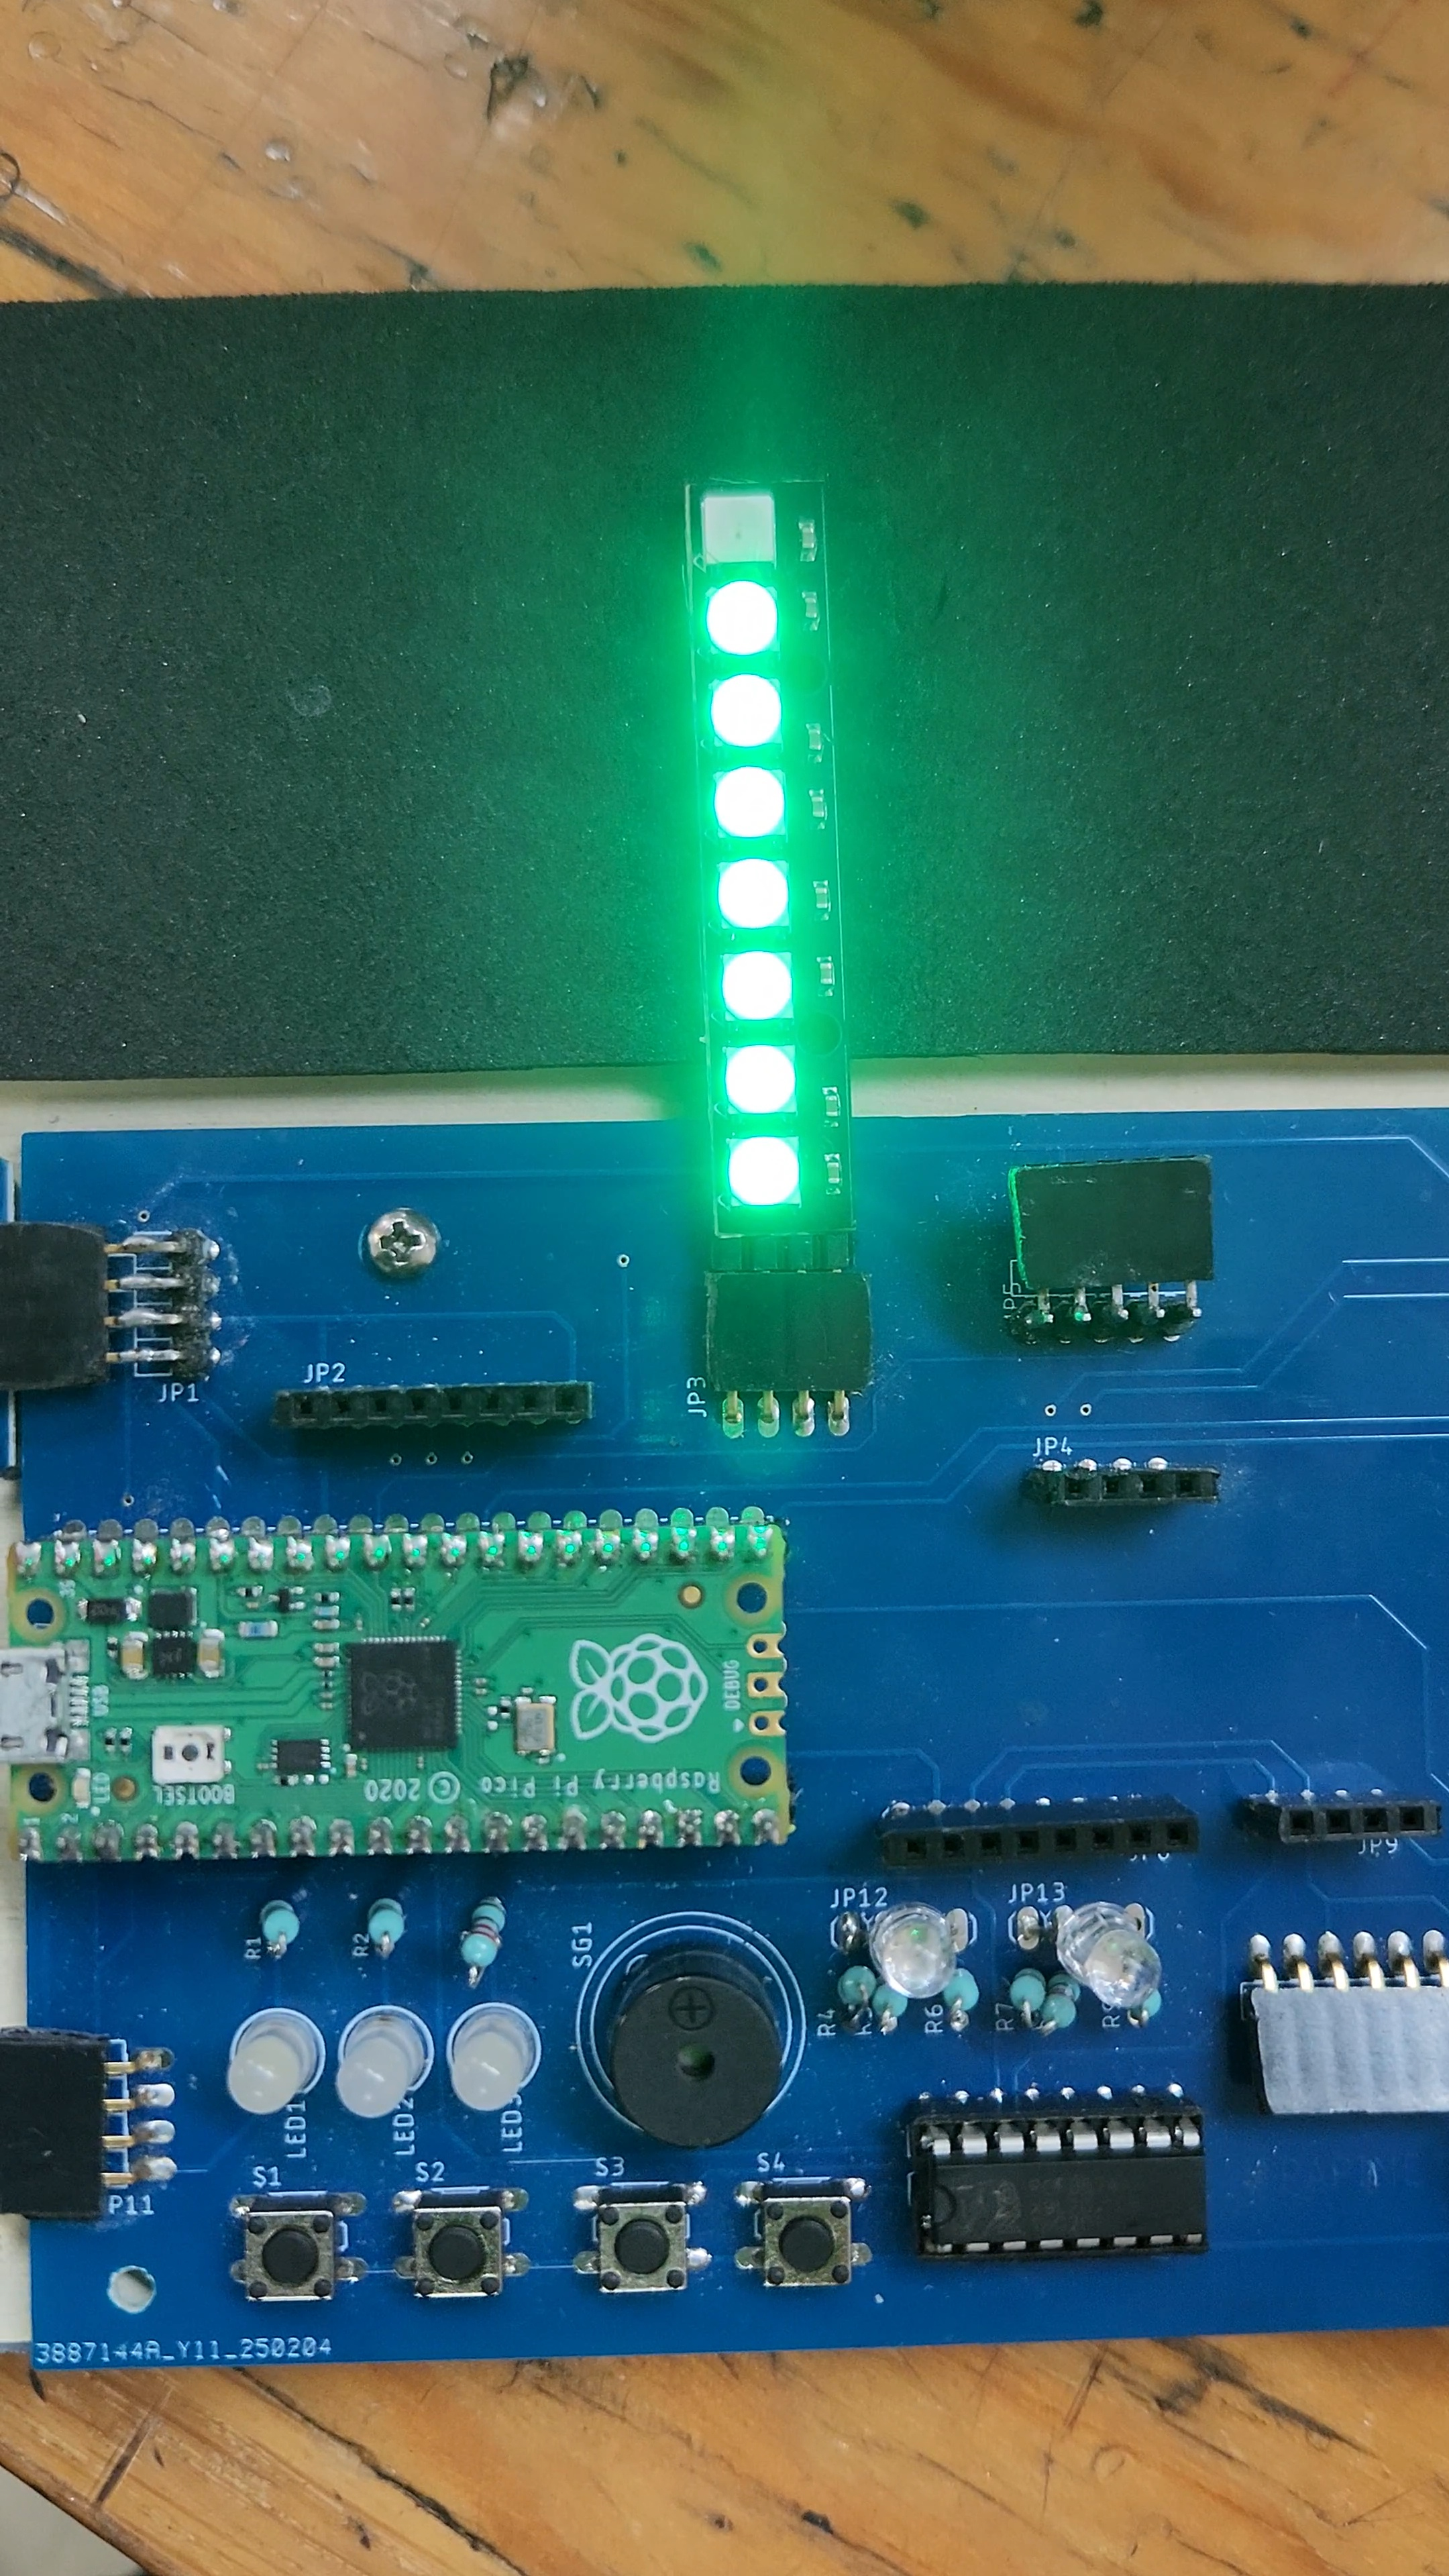
\includegraphics[width=\textwidth]{img/Actividad2/Act2_6.jpg}
        \caption{Posicion 7}
    \end{minipage}\hfill
    \begin{minipage}{0.3\textwidth}
        \centering
        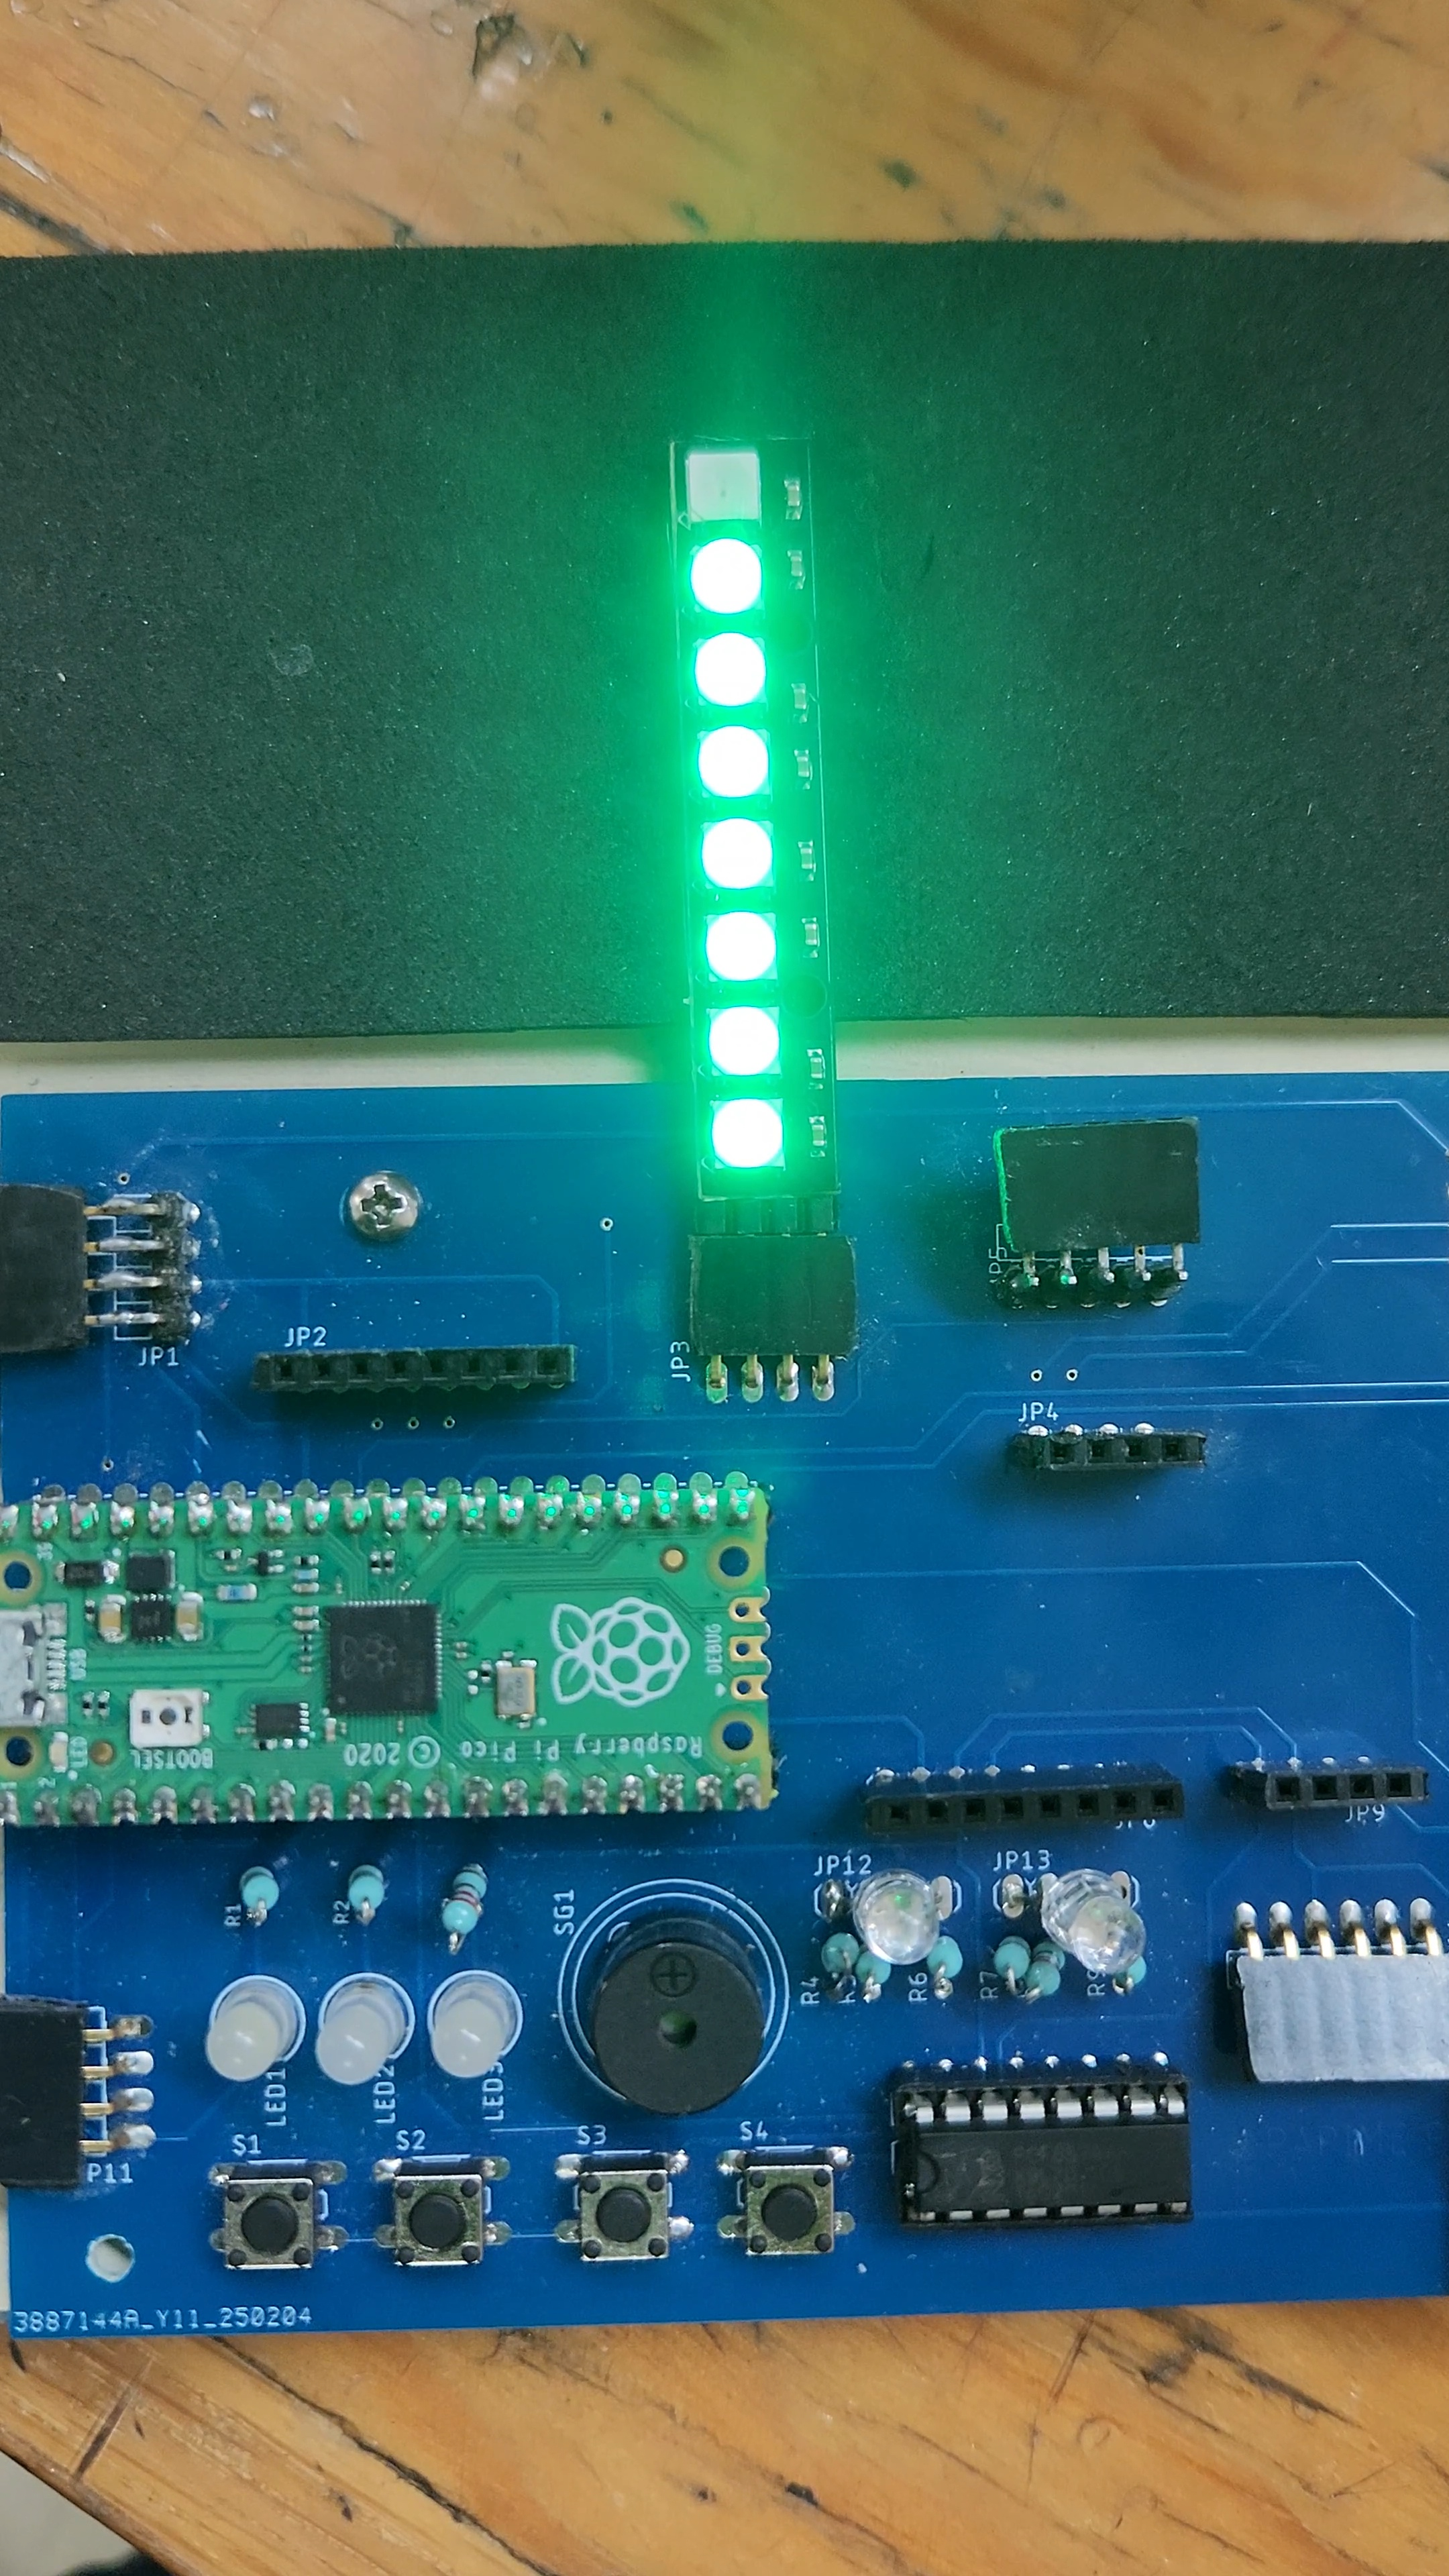
\includegraphics[width=\textwidth]{img/Actividad2/Act2_7.jpg}
        \caption{Posicion 9}
    \end{minipage}\hfill
    \begin{minipage}{0.3\textwidth}
        \centering
        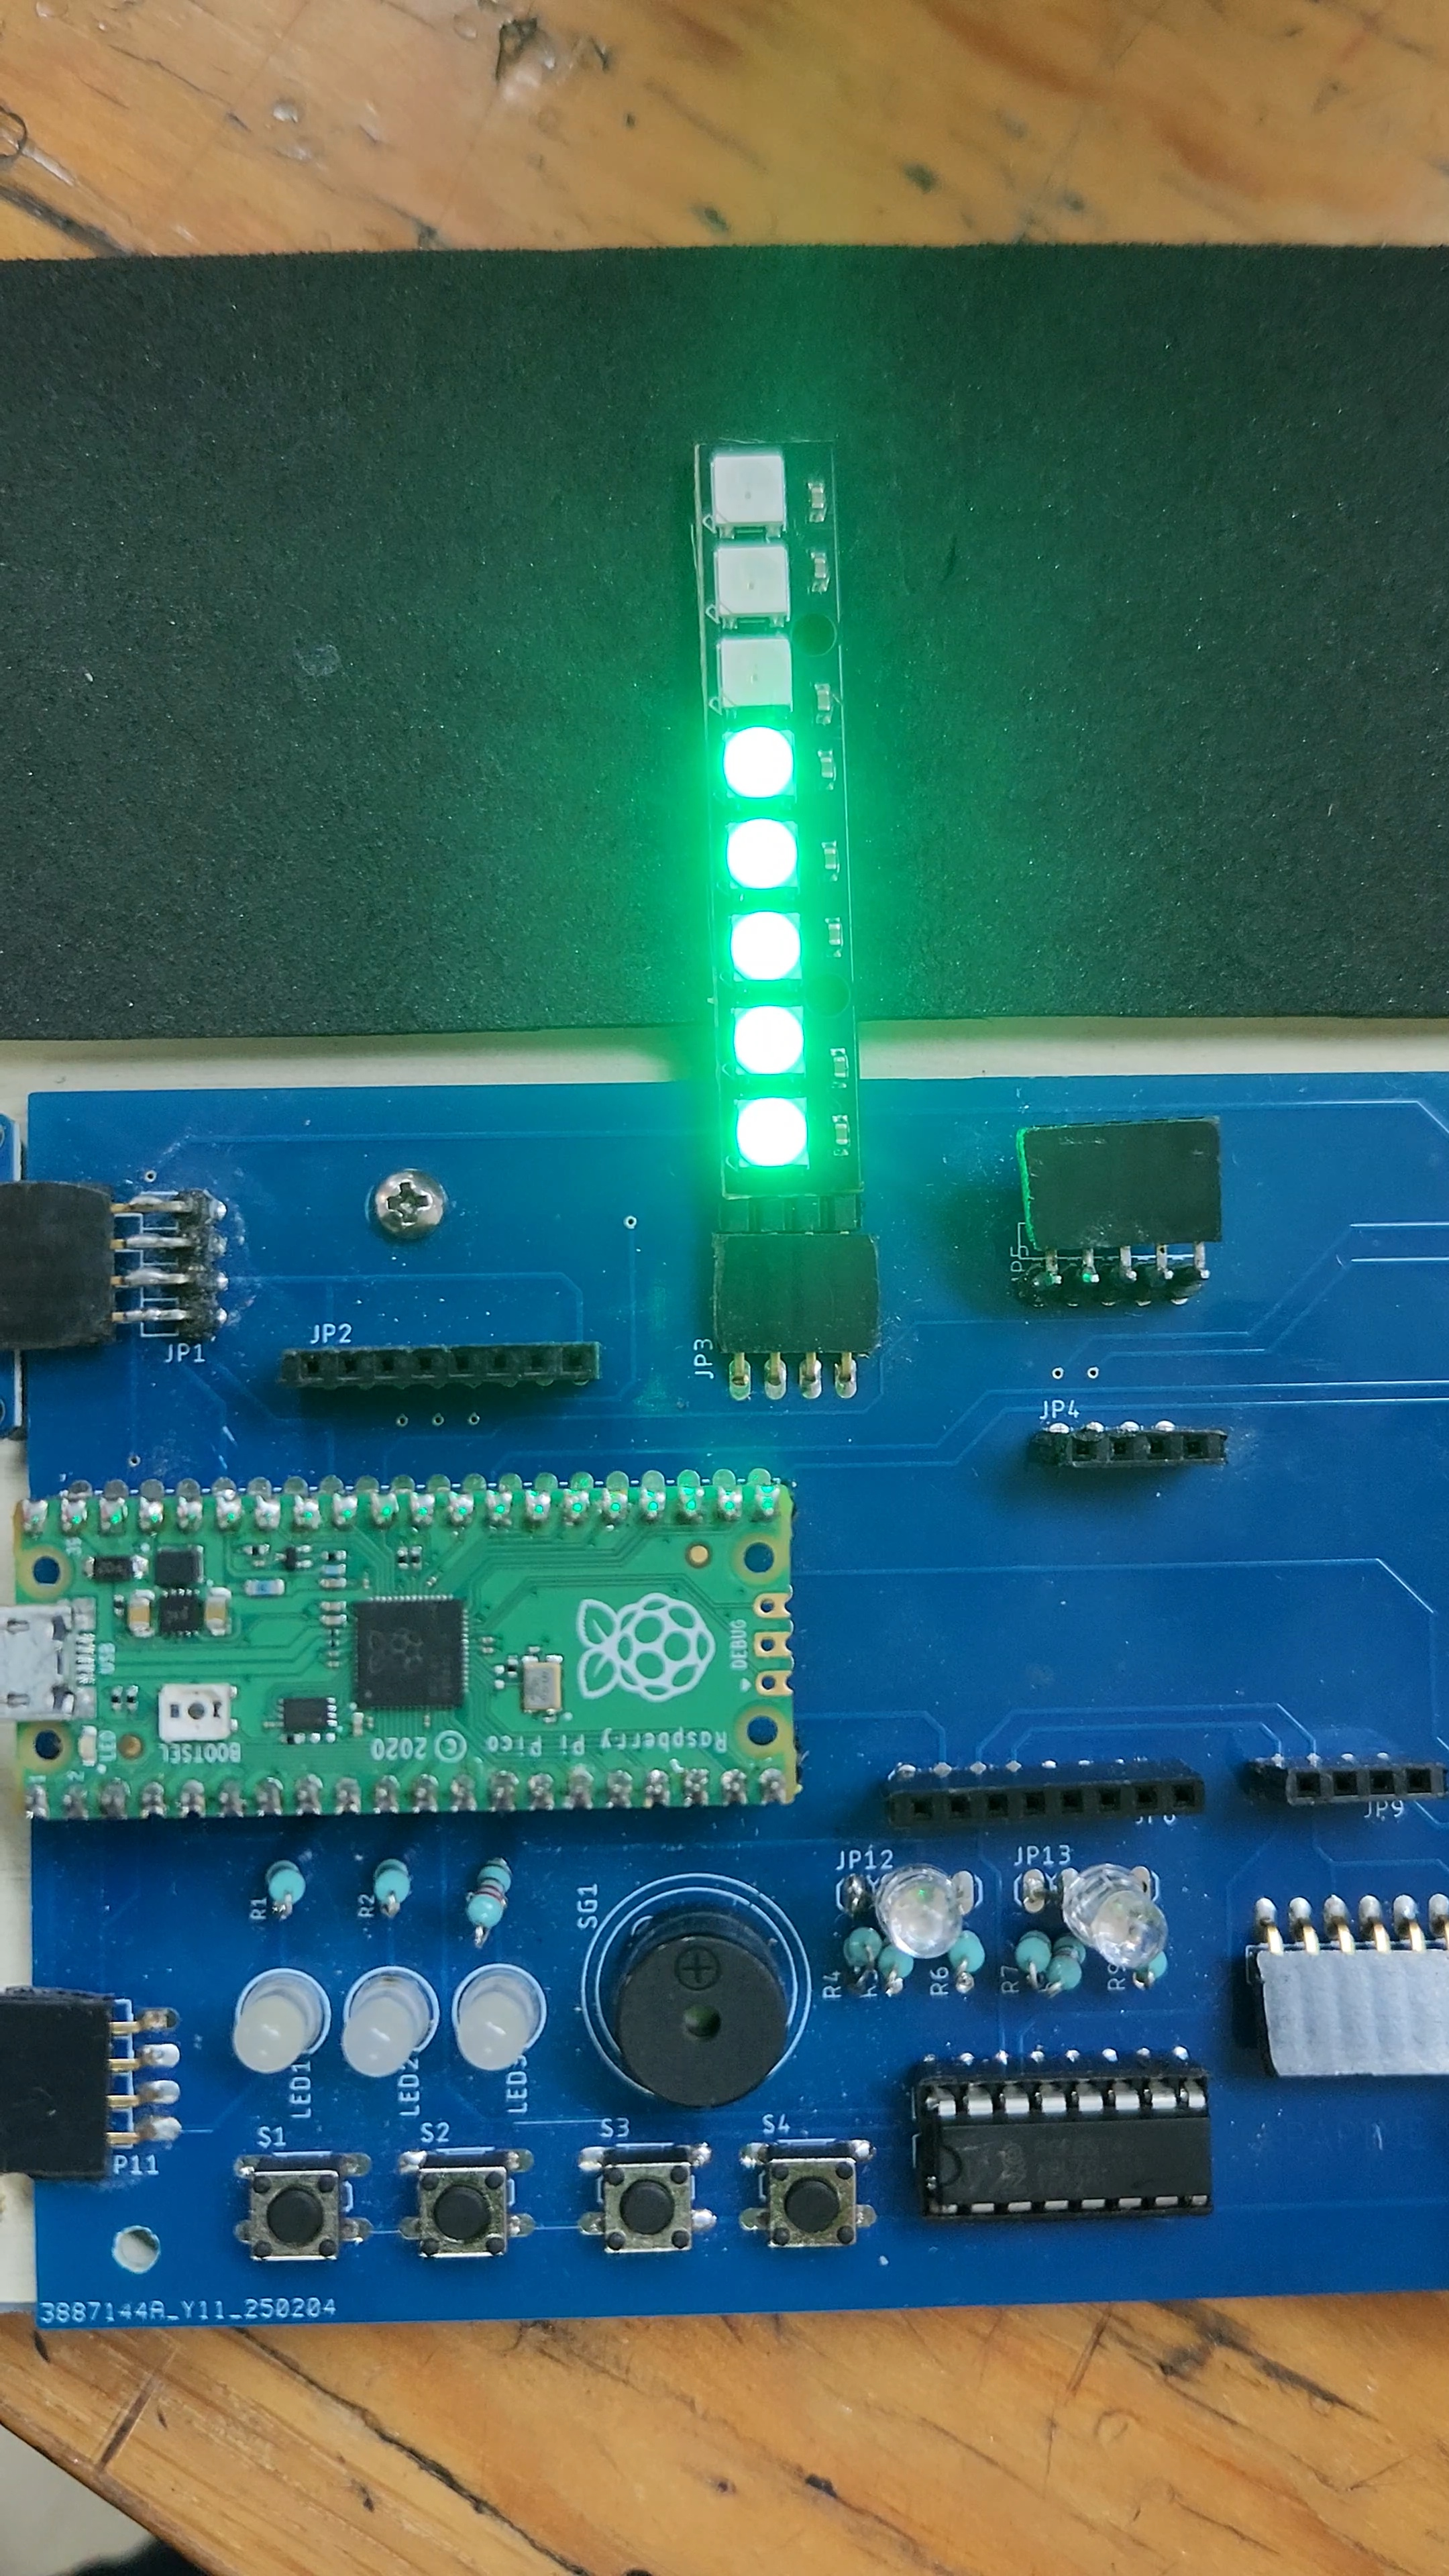
\includegraphics[width=\textwidth]{img/Actividad2/Act2_8.jpg}
        \caption{Posicion 11 }
    \end{minipage}
\end{figure}

\begin{figure}[H]
    \centering
    \begin{minipage}{0.3\textwidth}
        \centering
        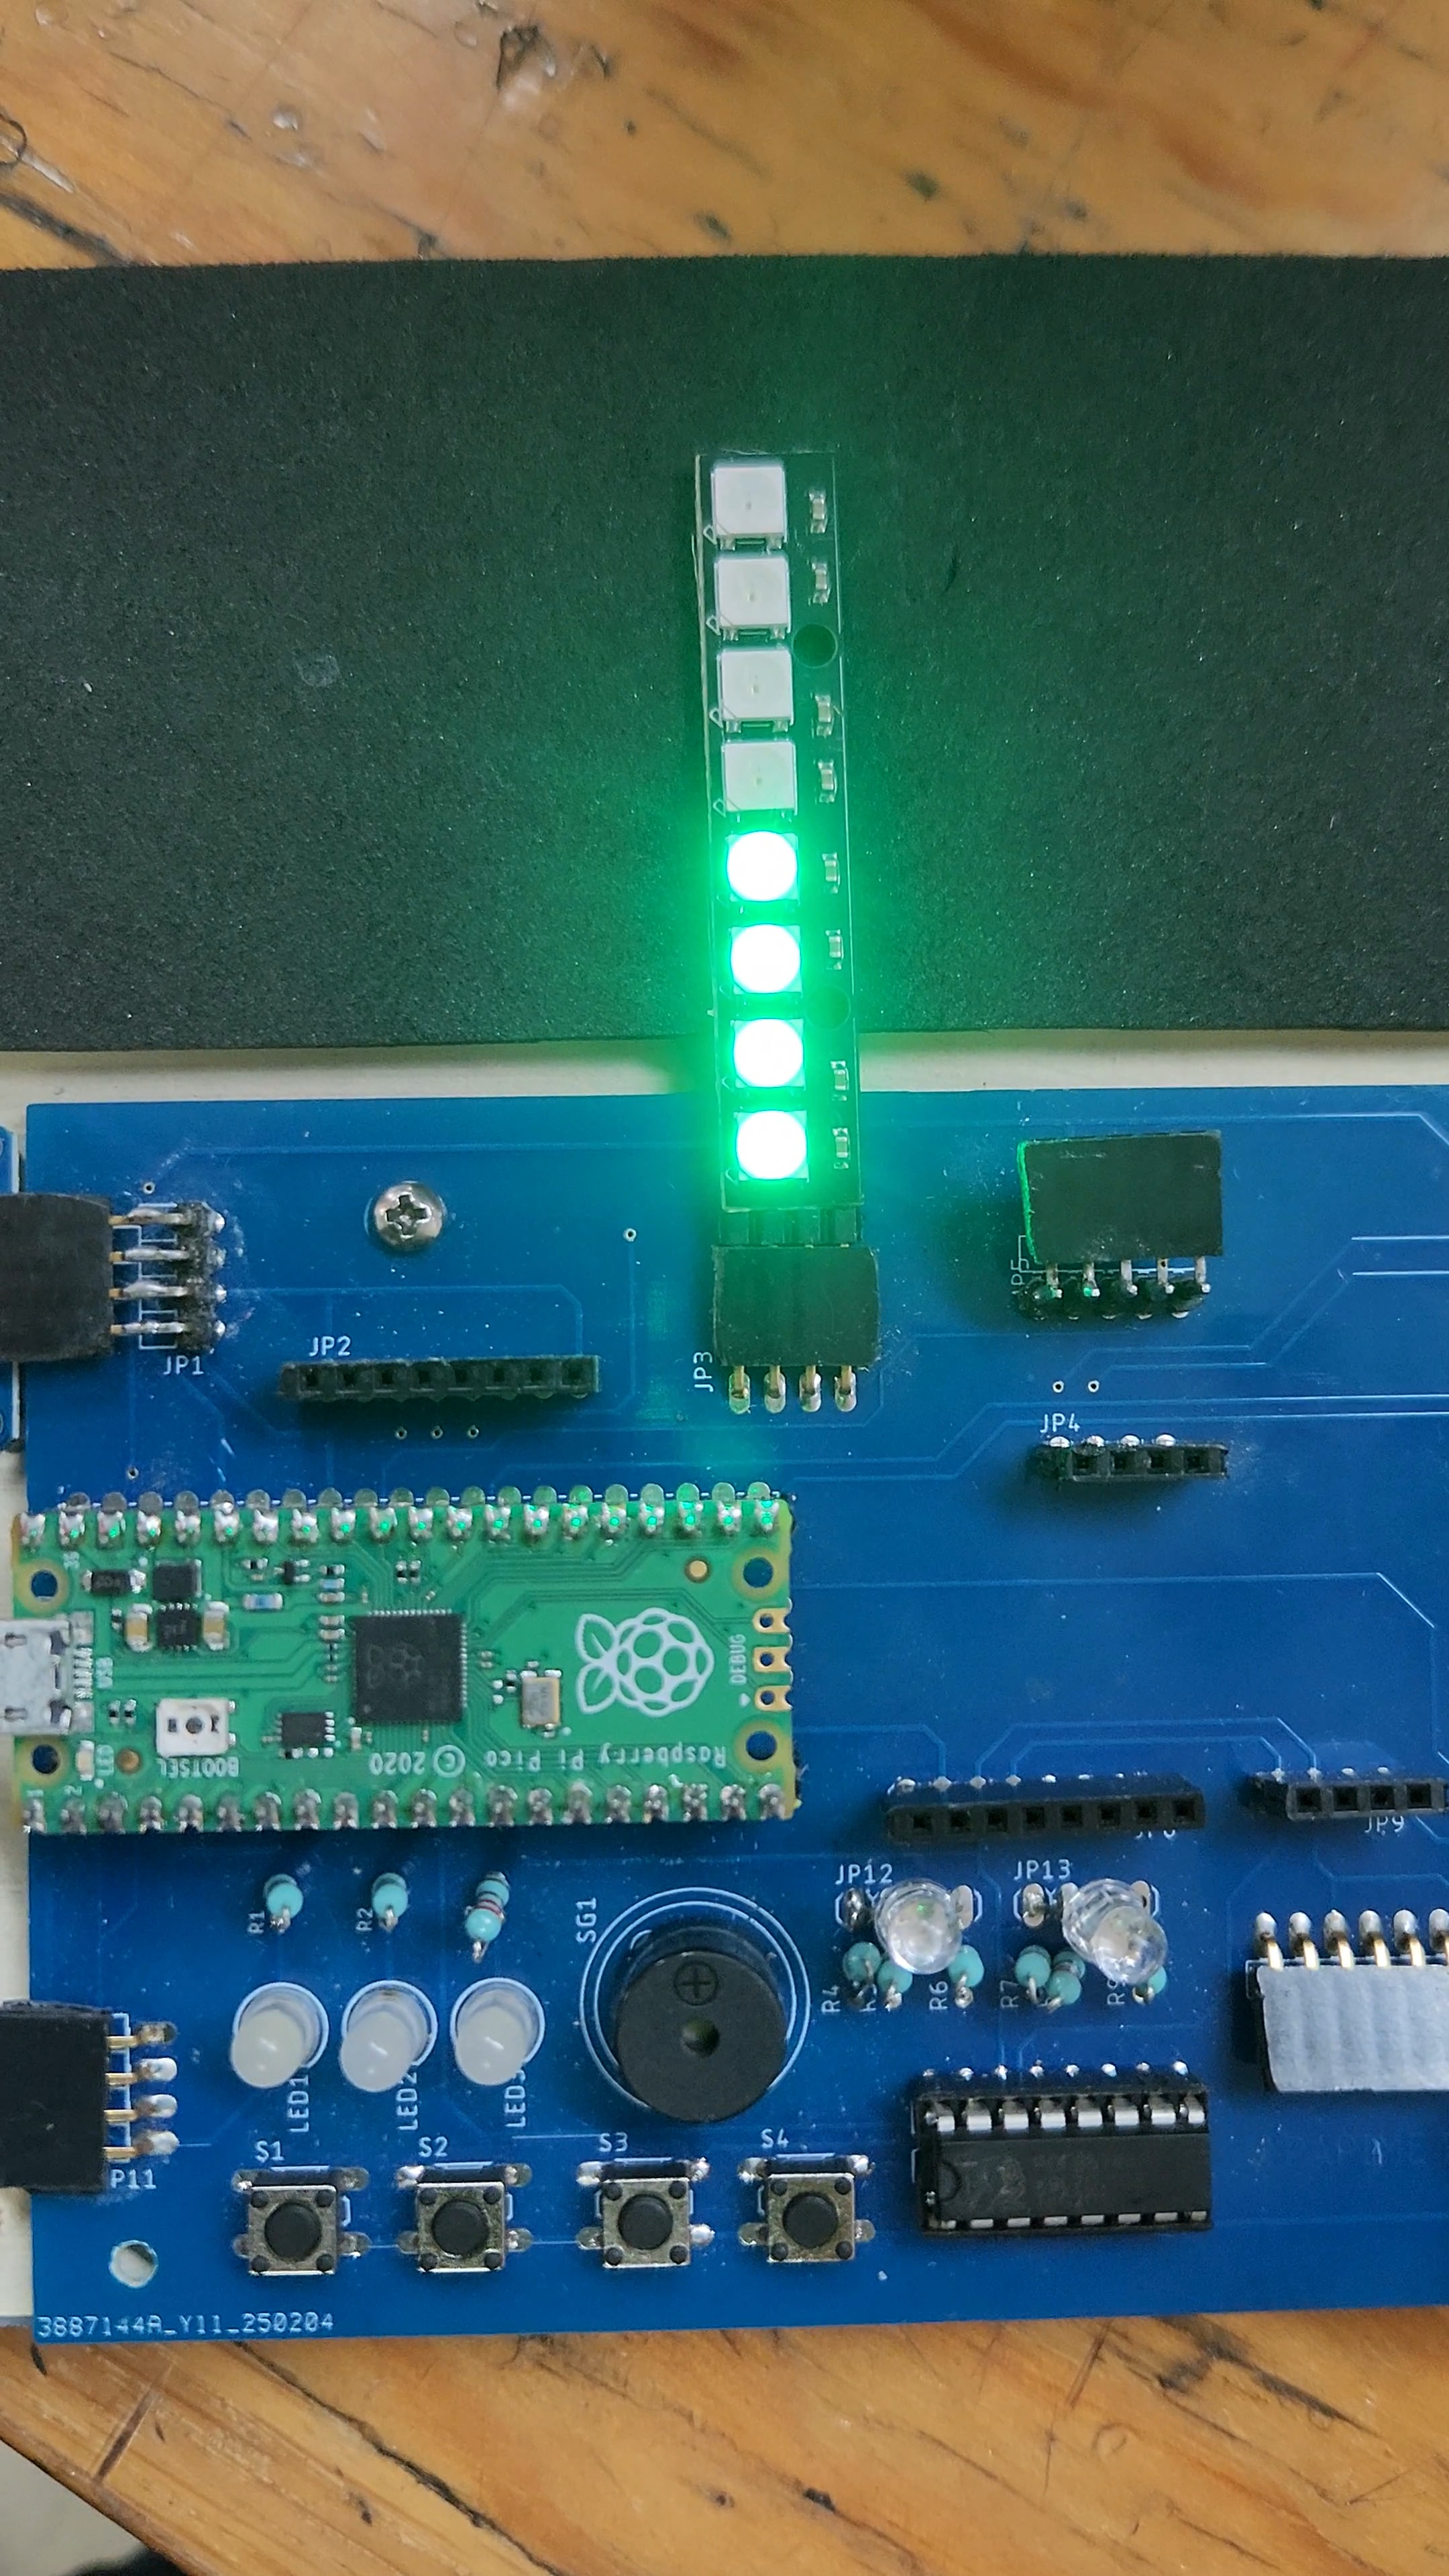
\includegraphics[width=\textwidth]{img/Actividad2/Act2_9.jpg}
        \caption{Posicion 12}
    \end{minipage}\hfill
    \begin{minipage}{0.3\textwidth}
        \centering
        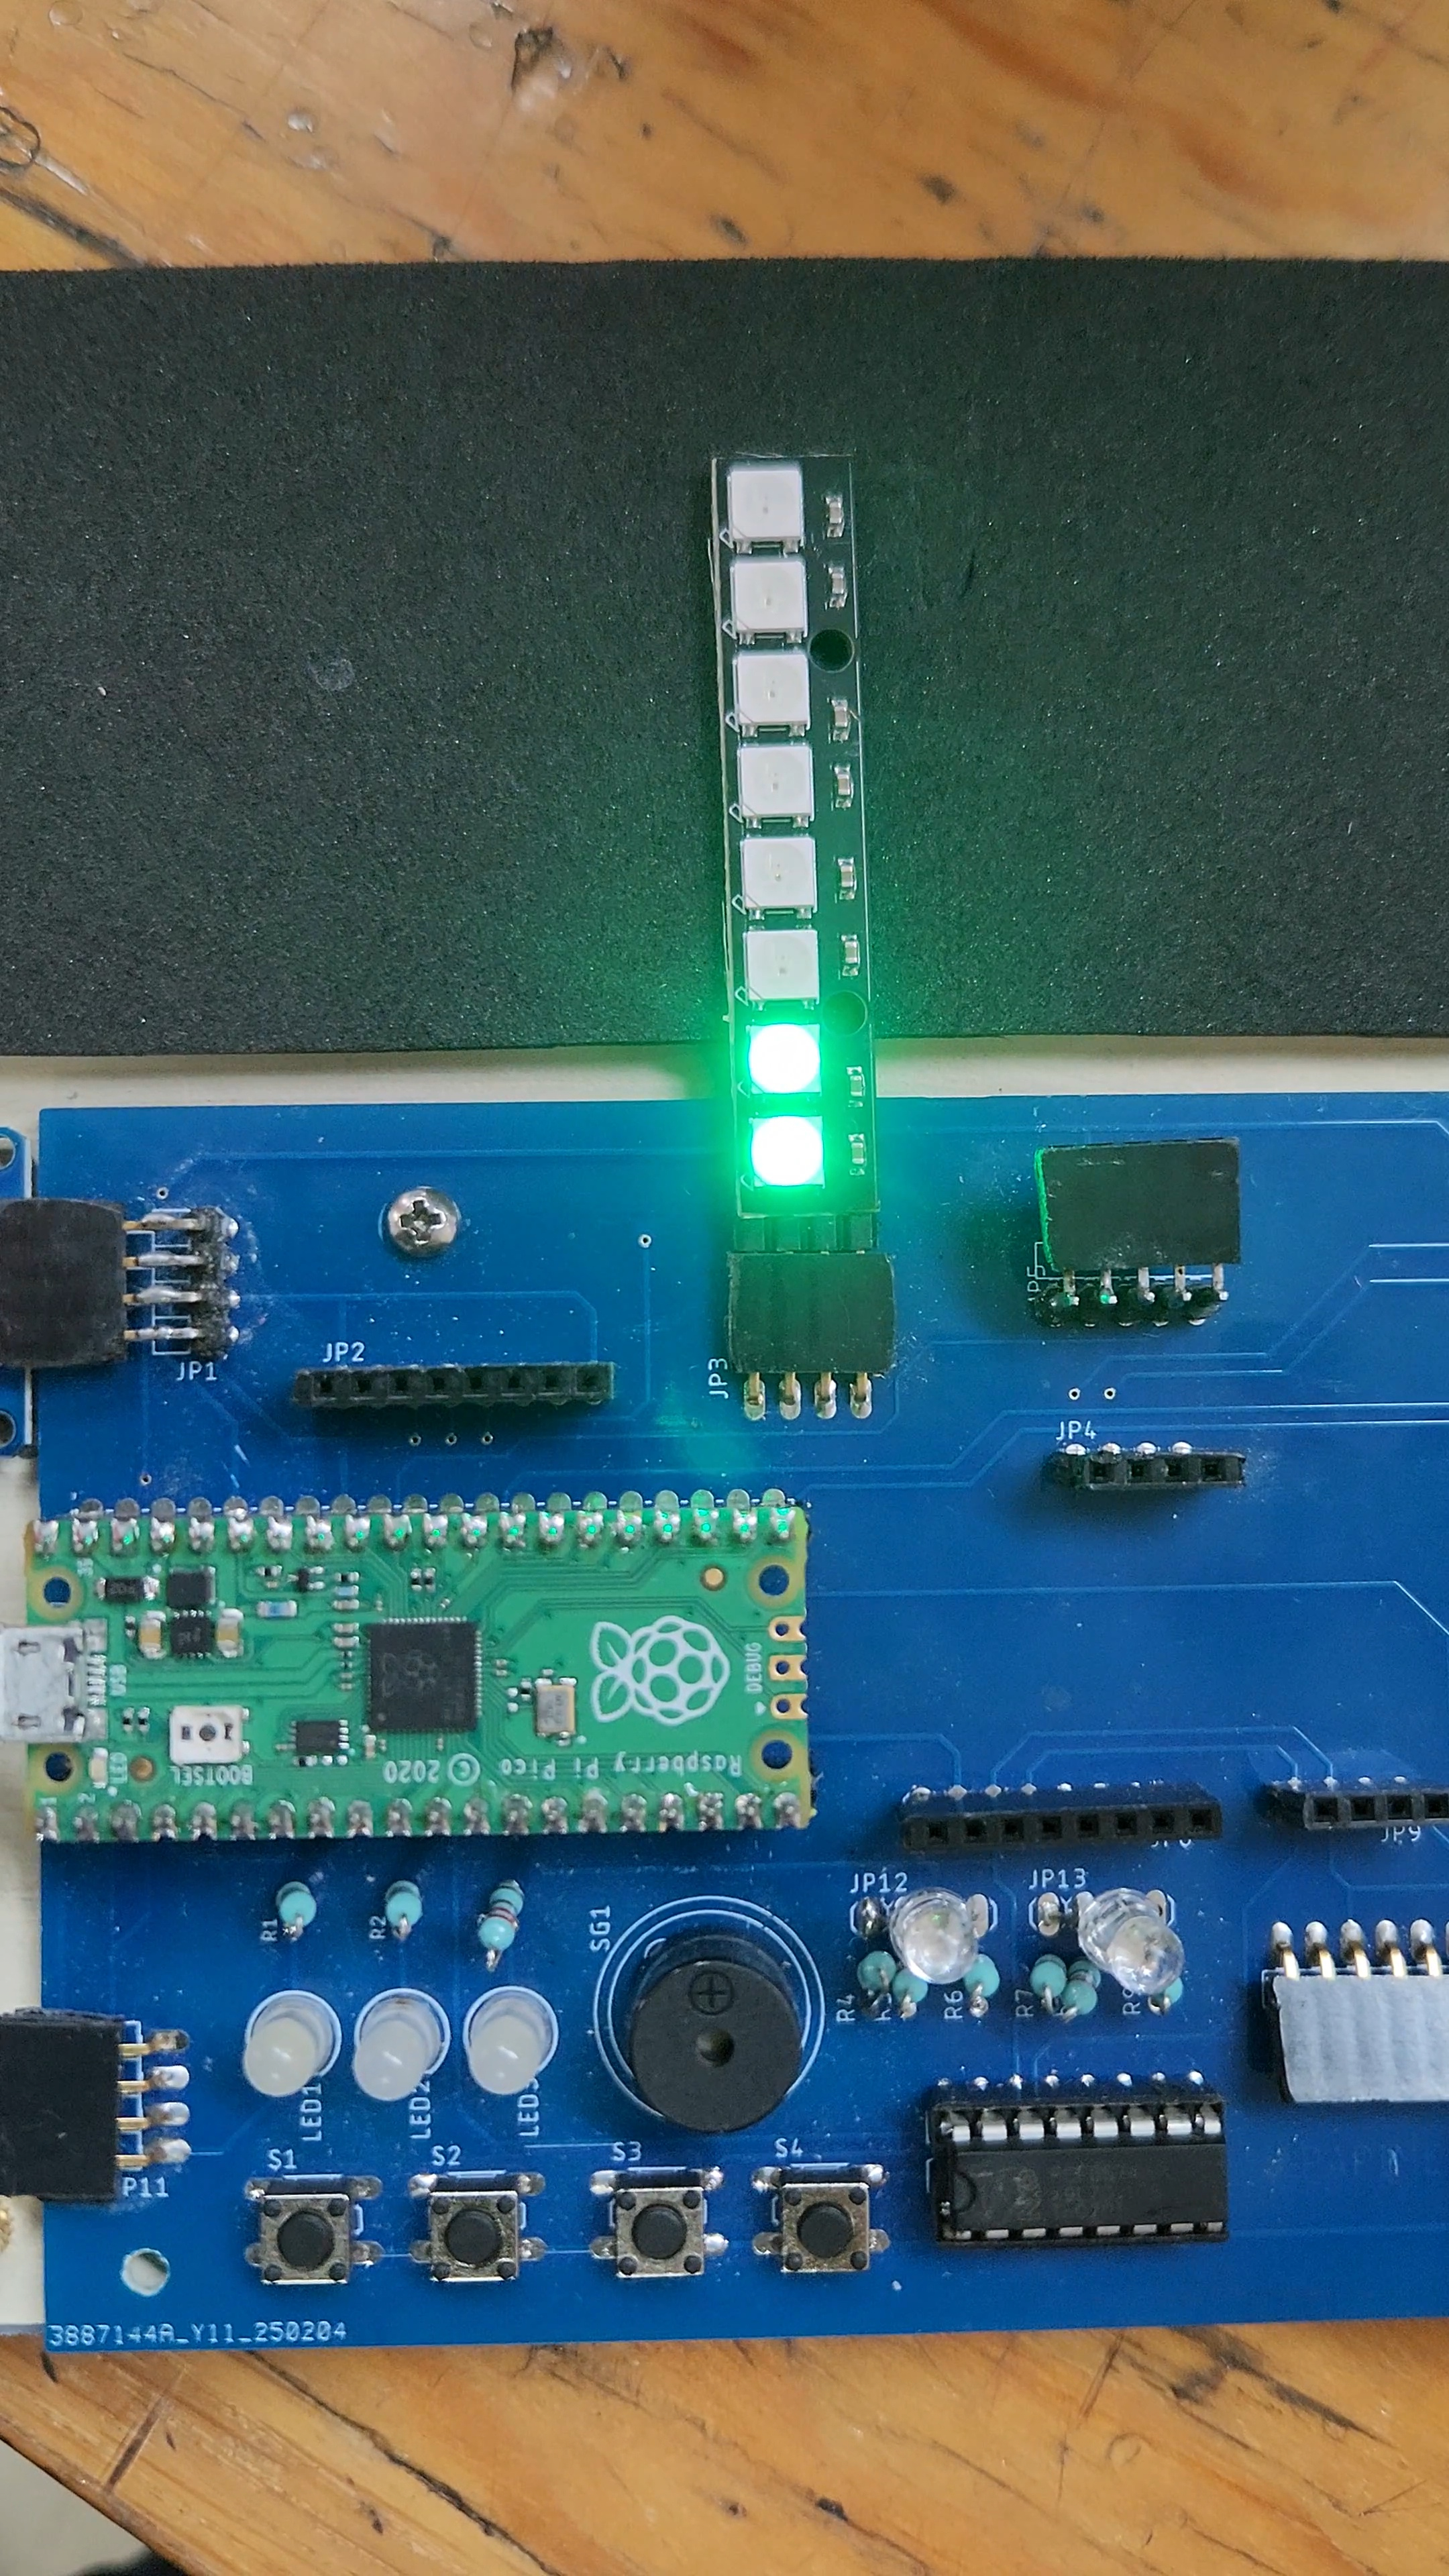
\includegraphics[width=\textwidth]{img/Actividad2/Act2_10.jpg}
        \caption{Posicion 14}
    \end{minipage}\hfill
    \begin{minipage}{0.3\textwidth}
        \centering
        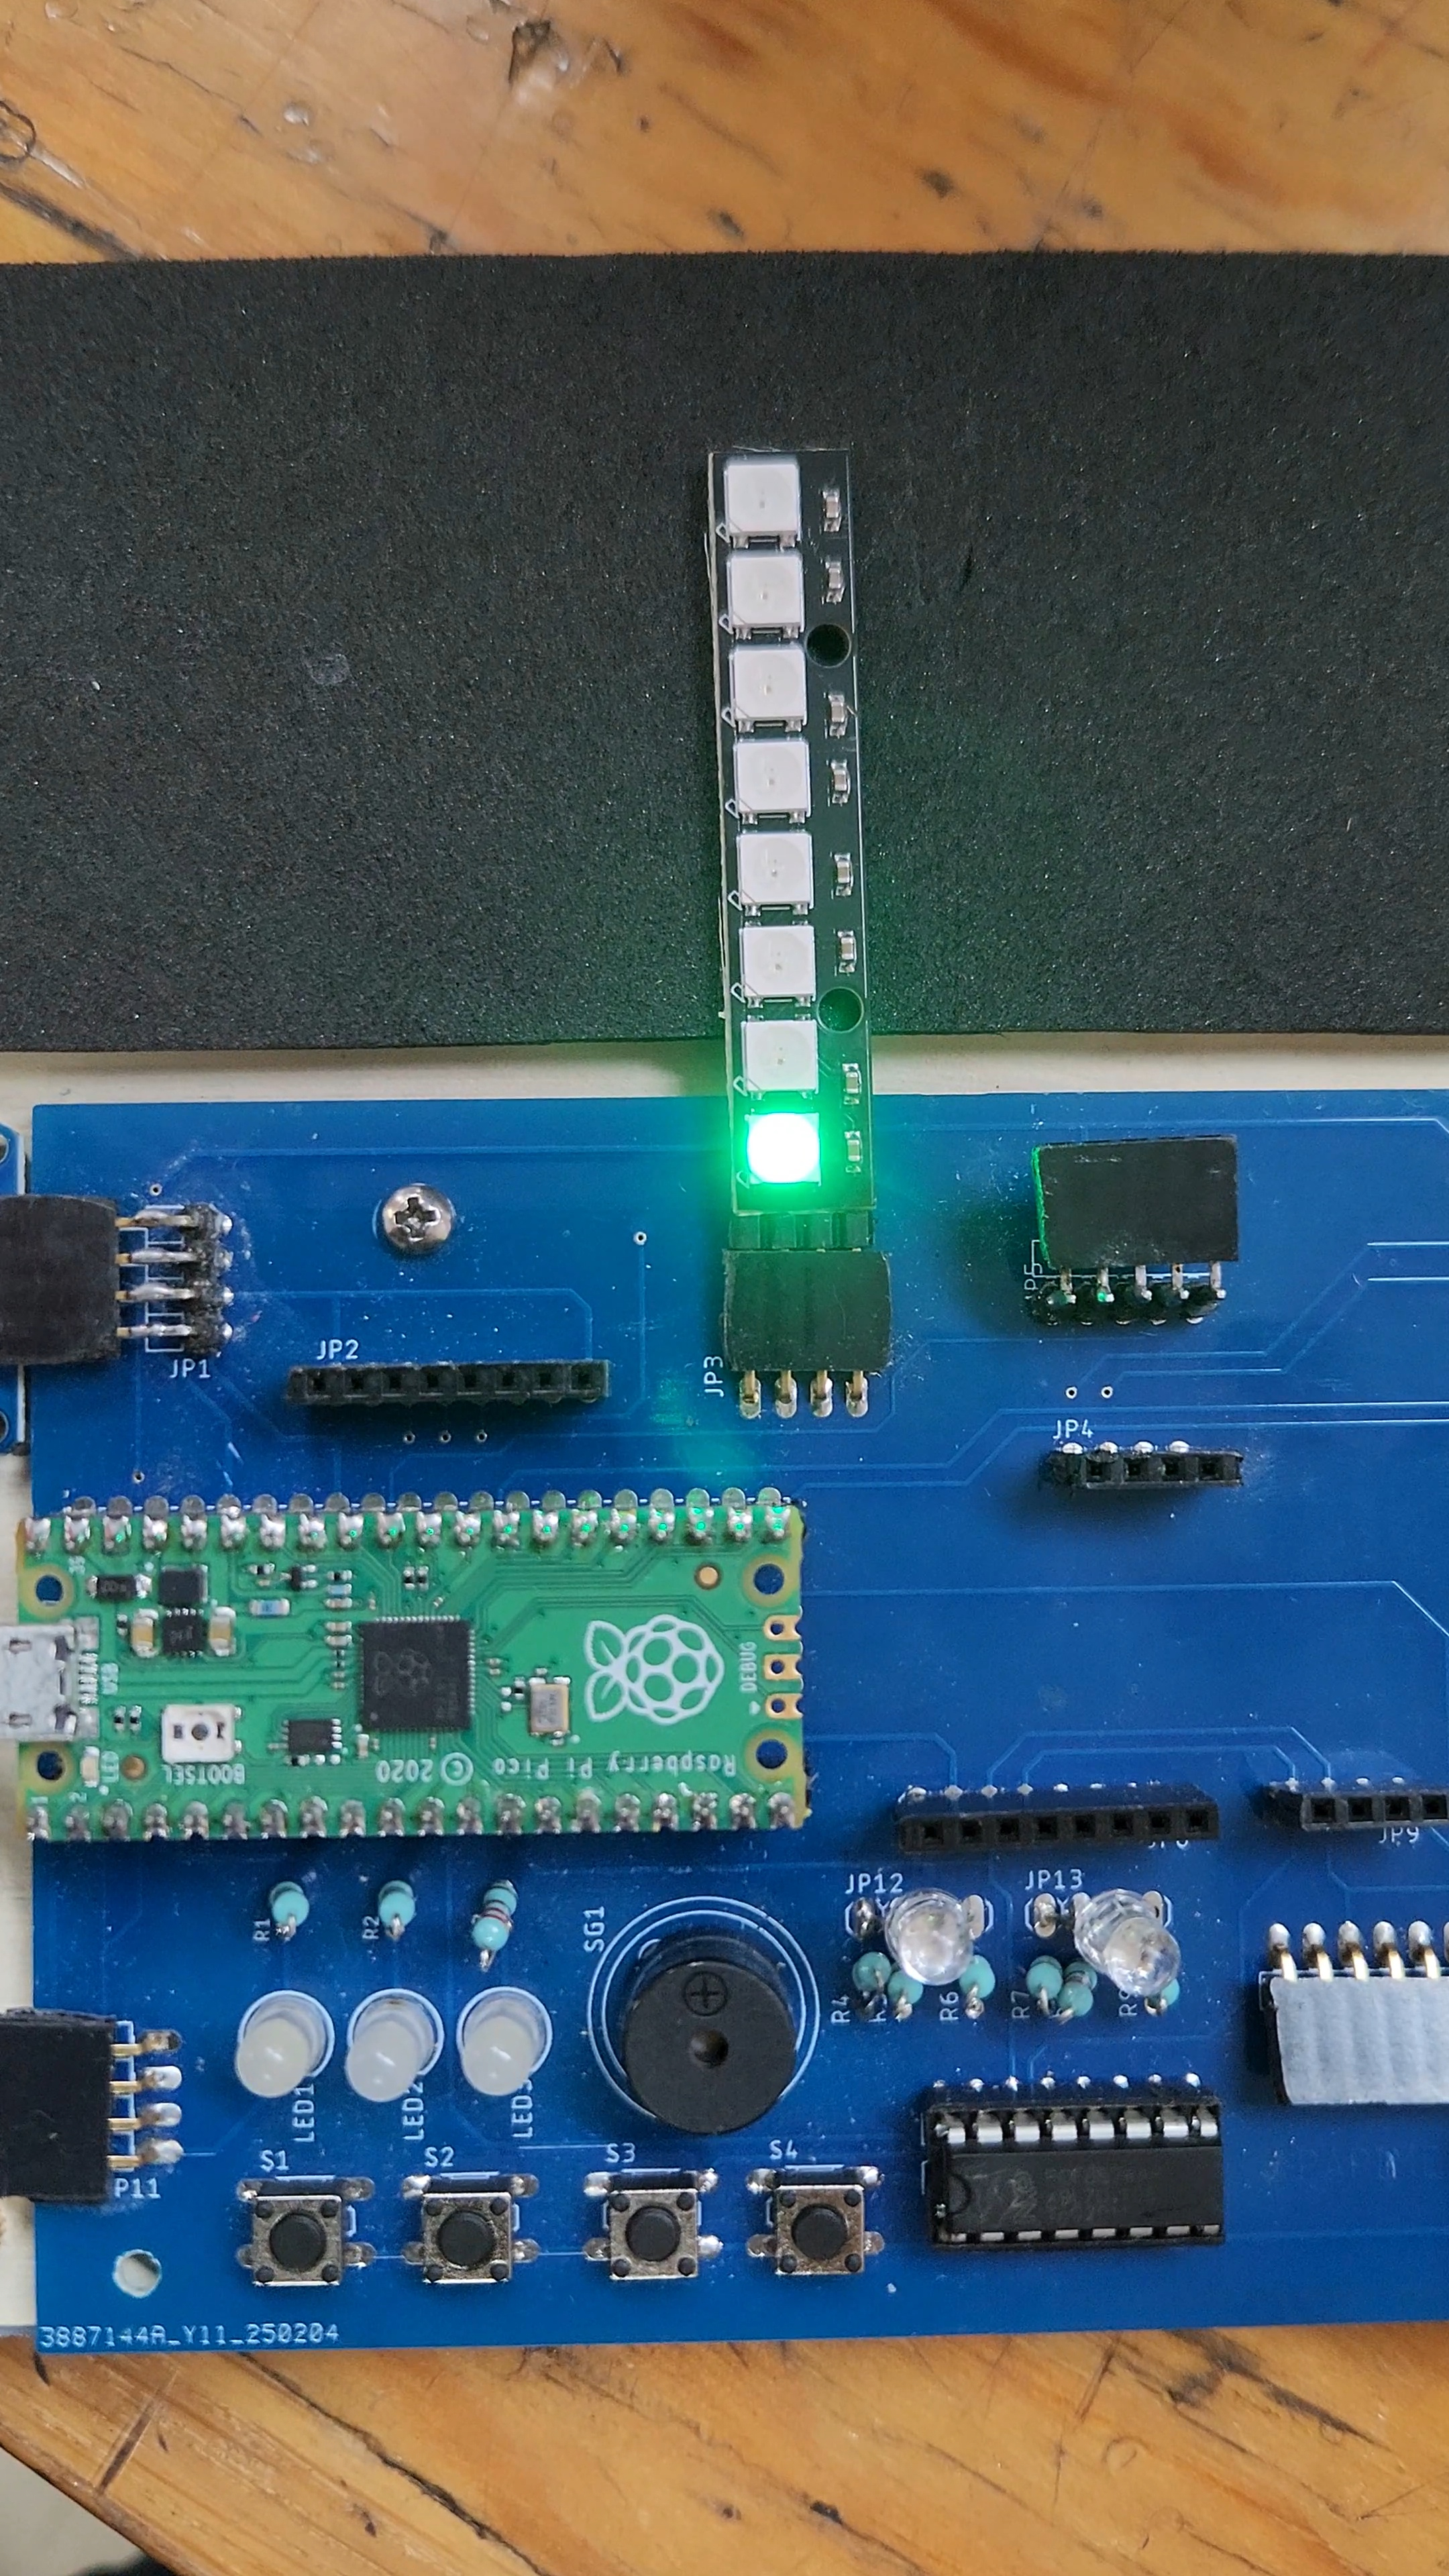
\includegraphics[width=\textwidth]{img/Actividad2/Act2_11.jpg}
        \caption{Posicion 15}
    \end{minipage}
\end{figure}

% ==========================================
% BLOQUE 3: Color Azul (15 imagenes)
% ==========================================
\textbf{Secuencia en color azul}

\begin{figure}[H]
    \centering
    \begin{minipage}{0.3\textwidth}
        \centering
        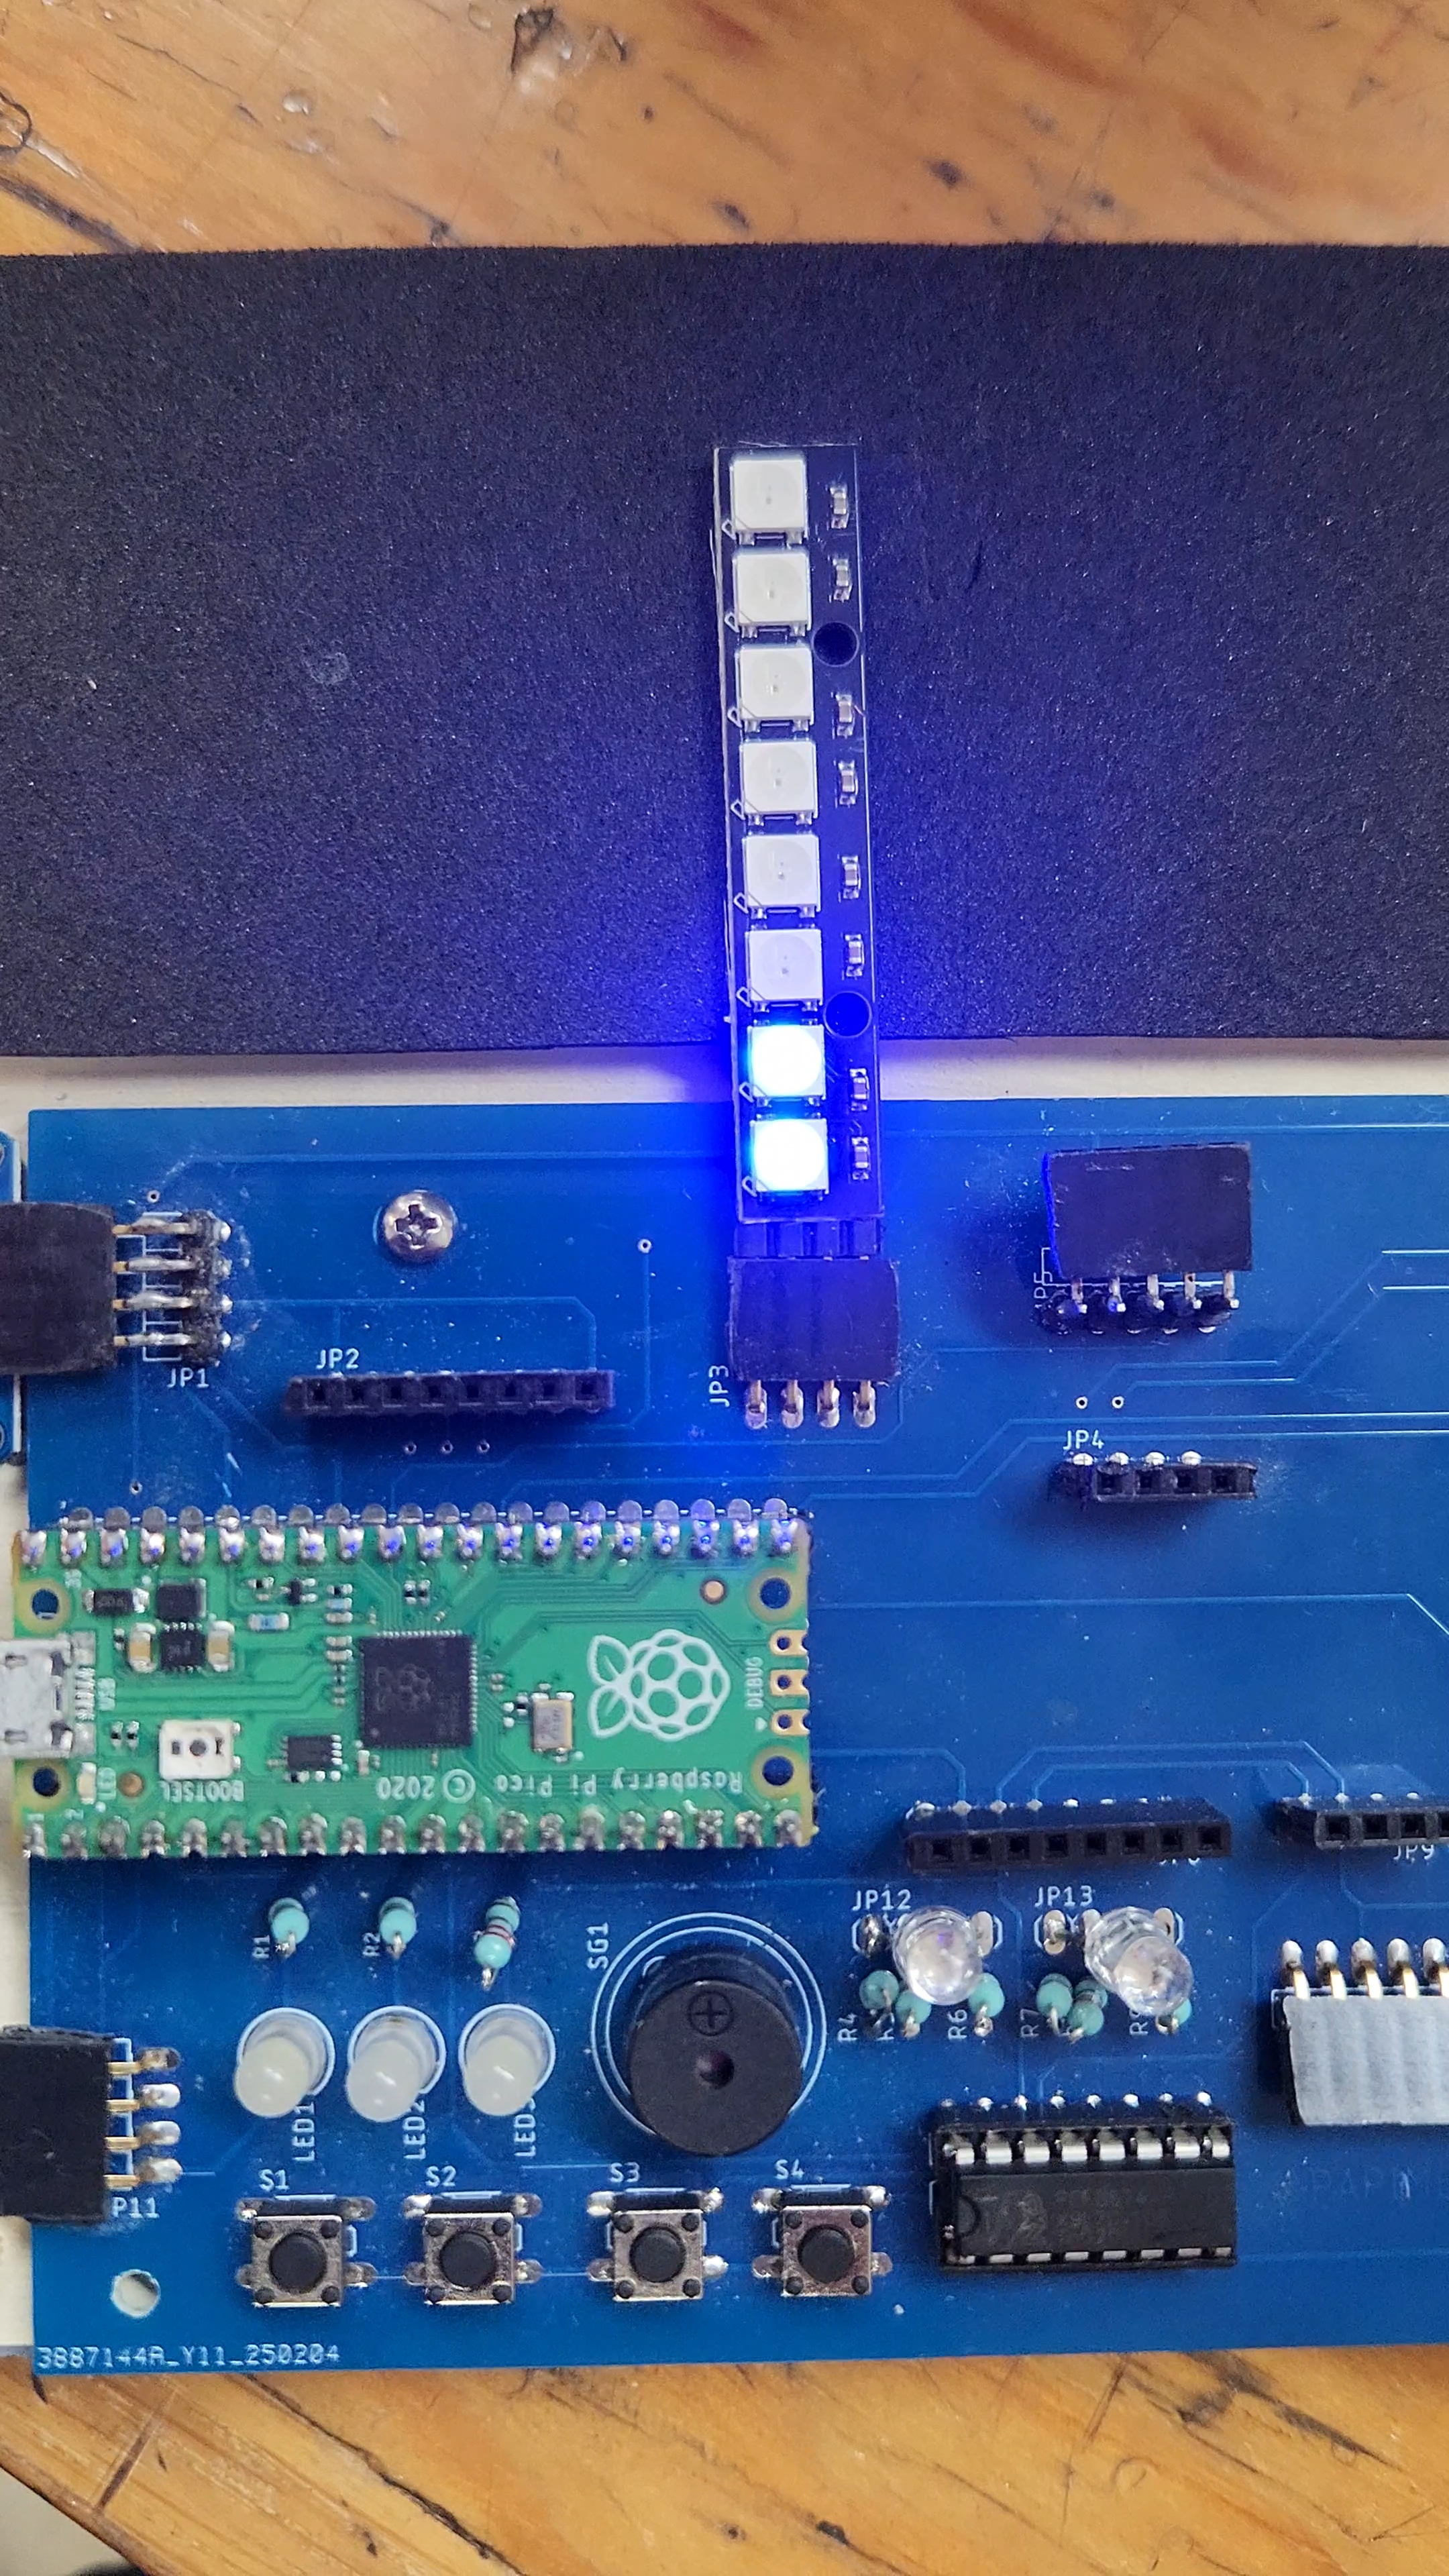
\includegraphics[width=\textwidth]{img/Actividad2/Act2_13.jpg}
        \caption{Posicion 2}
    \end{minipage}\hfill
    \begin{minipage}{0.3\textwidth}
        \centering
        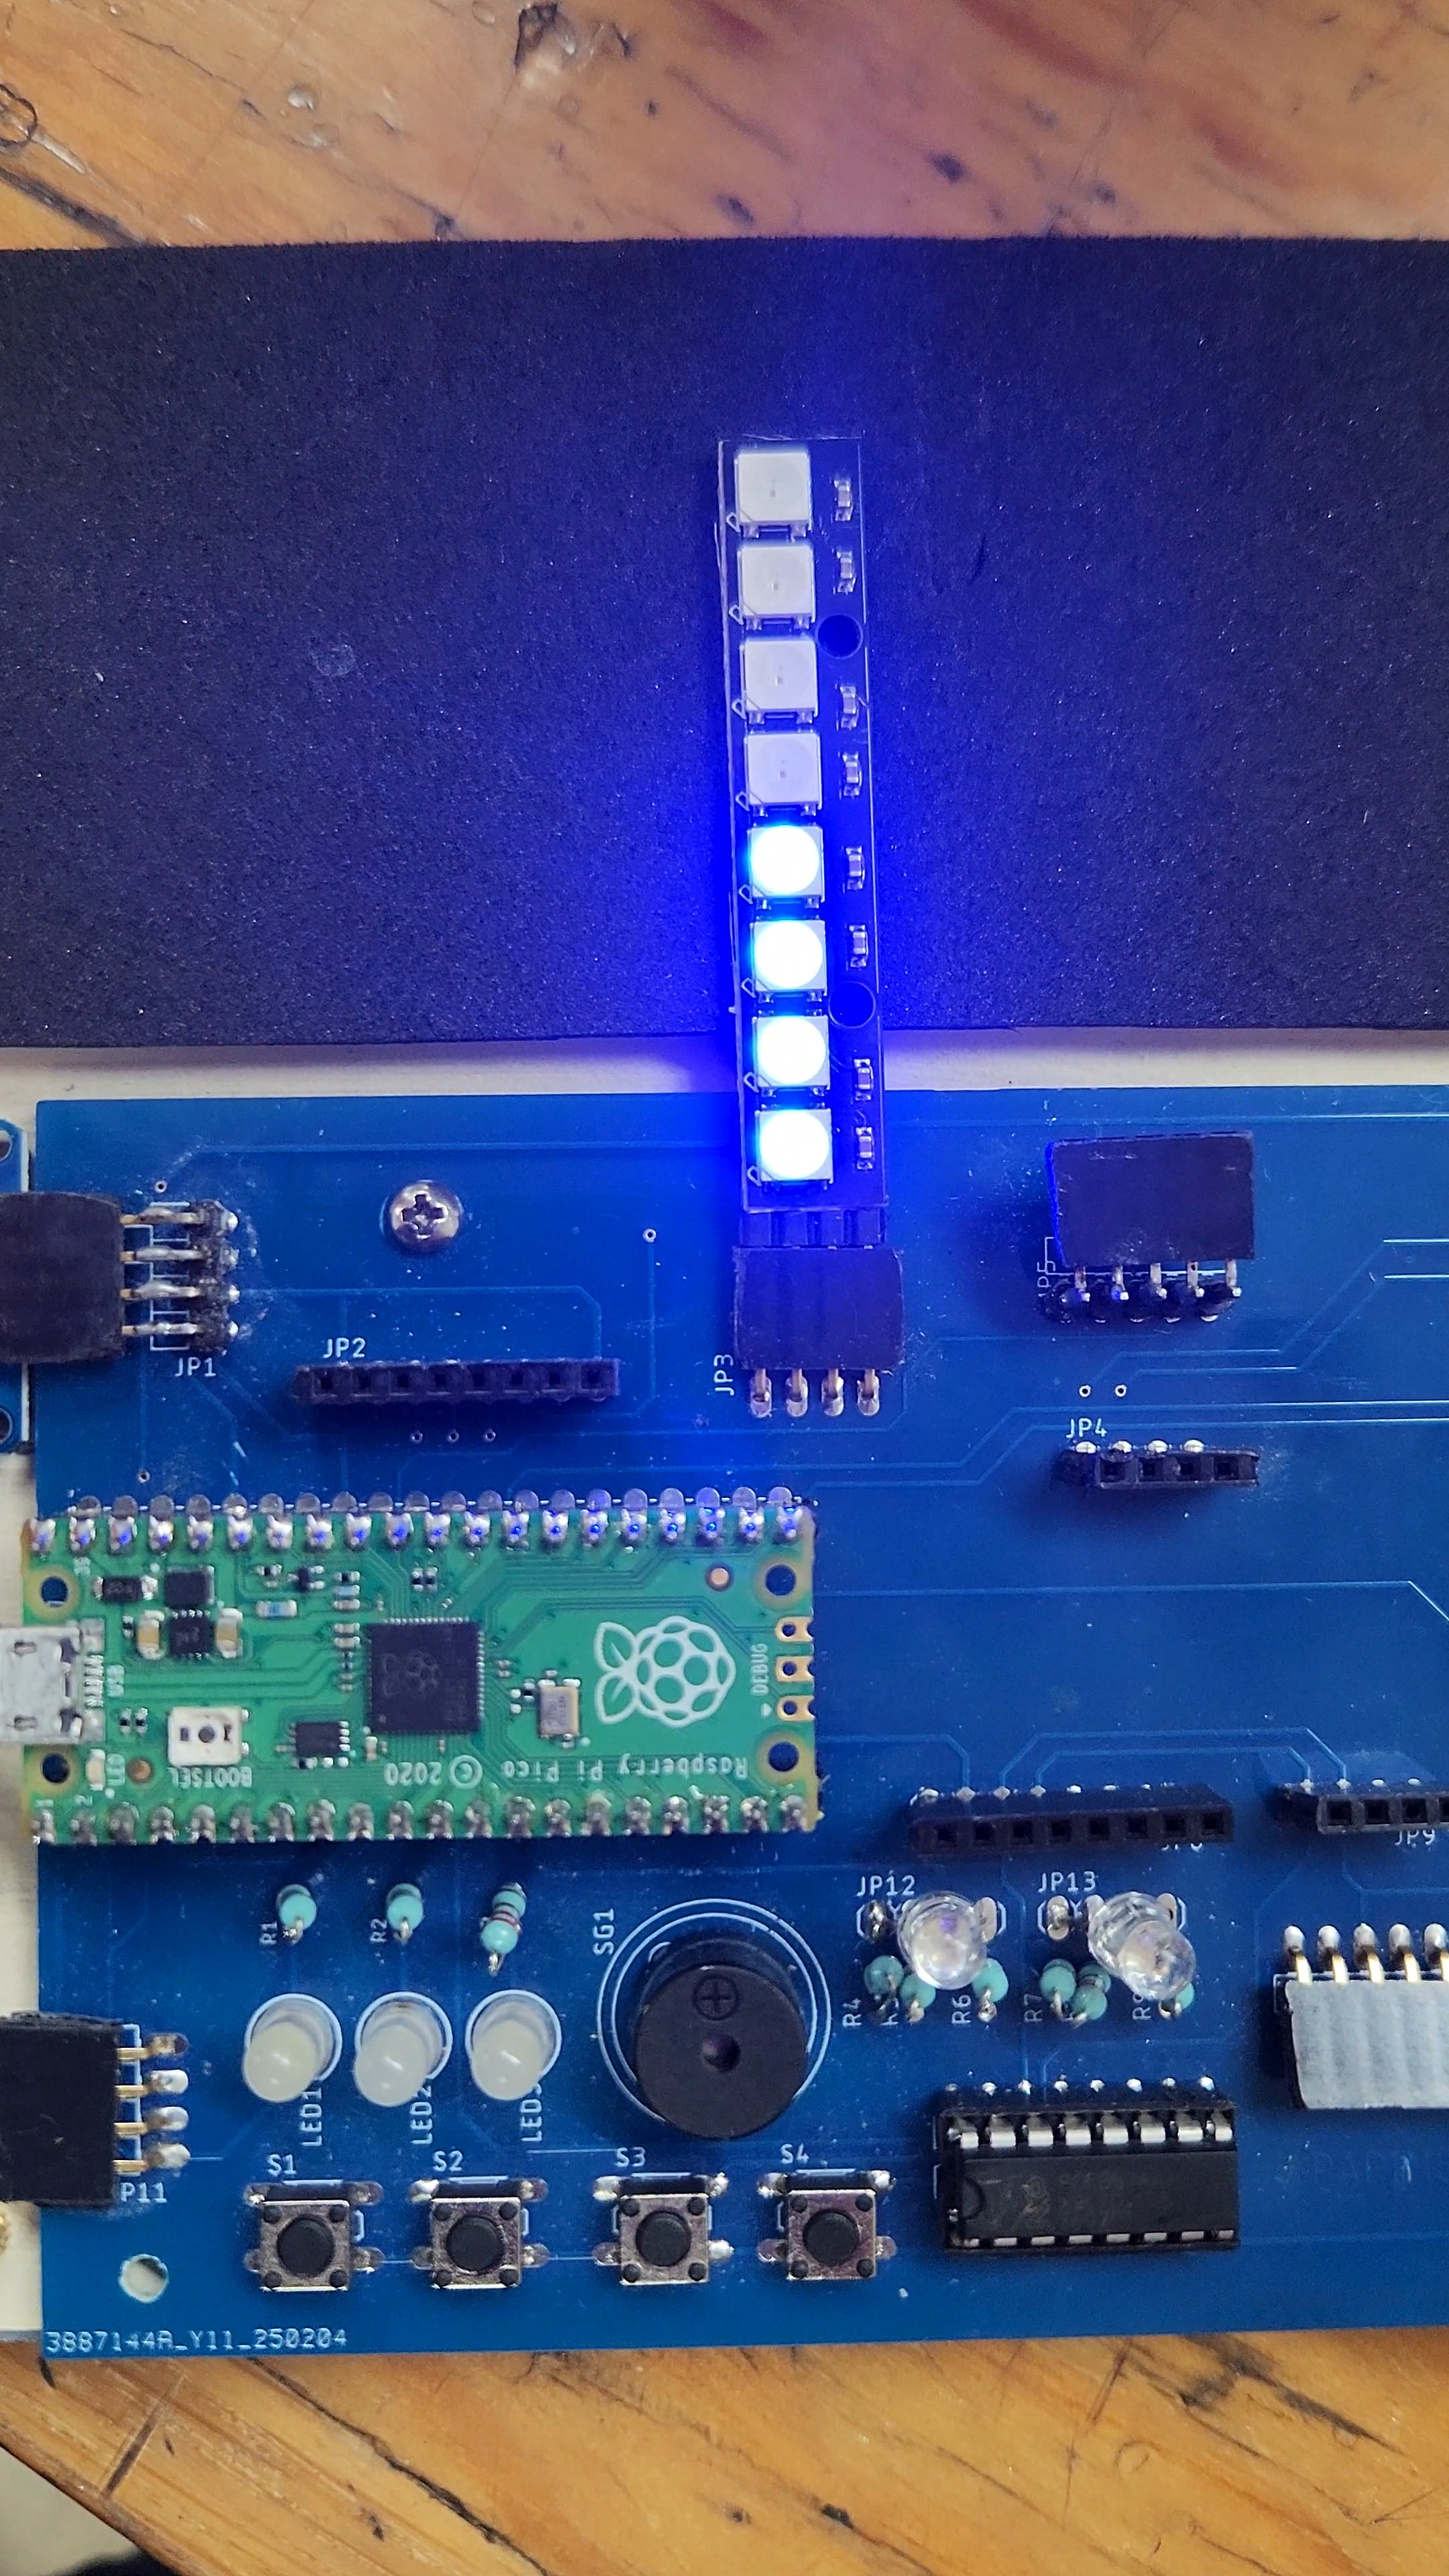
\includegraphics[width=\textwidth]{img/Actividad2/Act2_14.jpg}
        \caption{Posicion 4}
    \end{minipage}\hfill
    \begin{minipage}{0.3\textwidth}
        \centering
        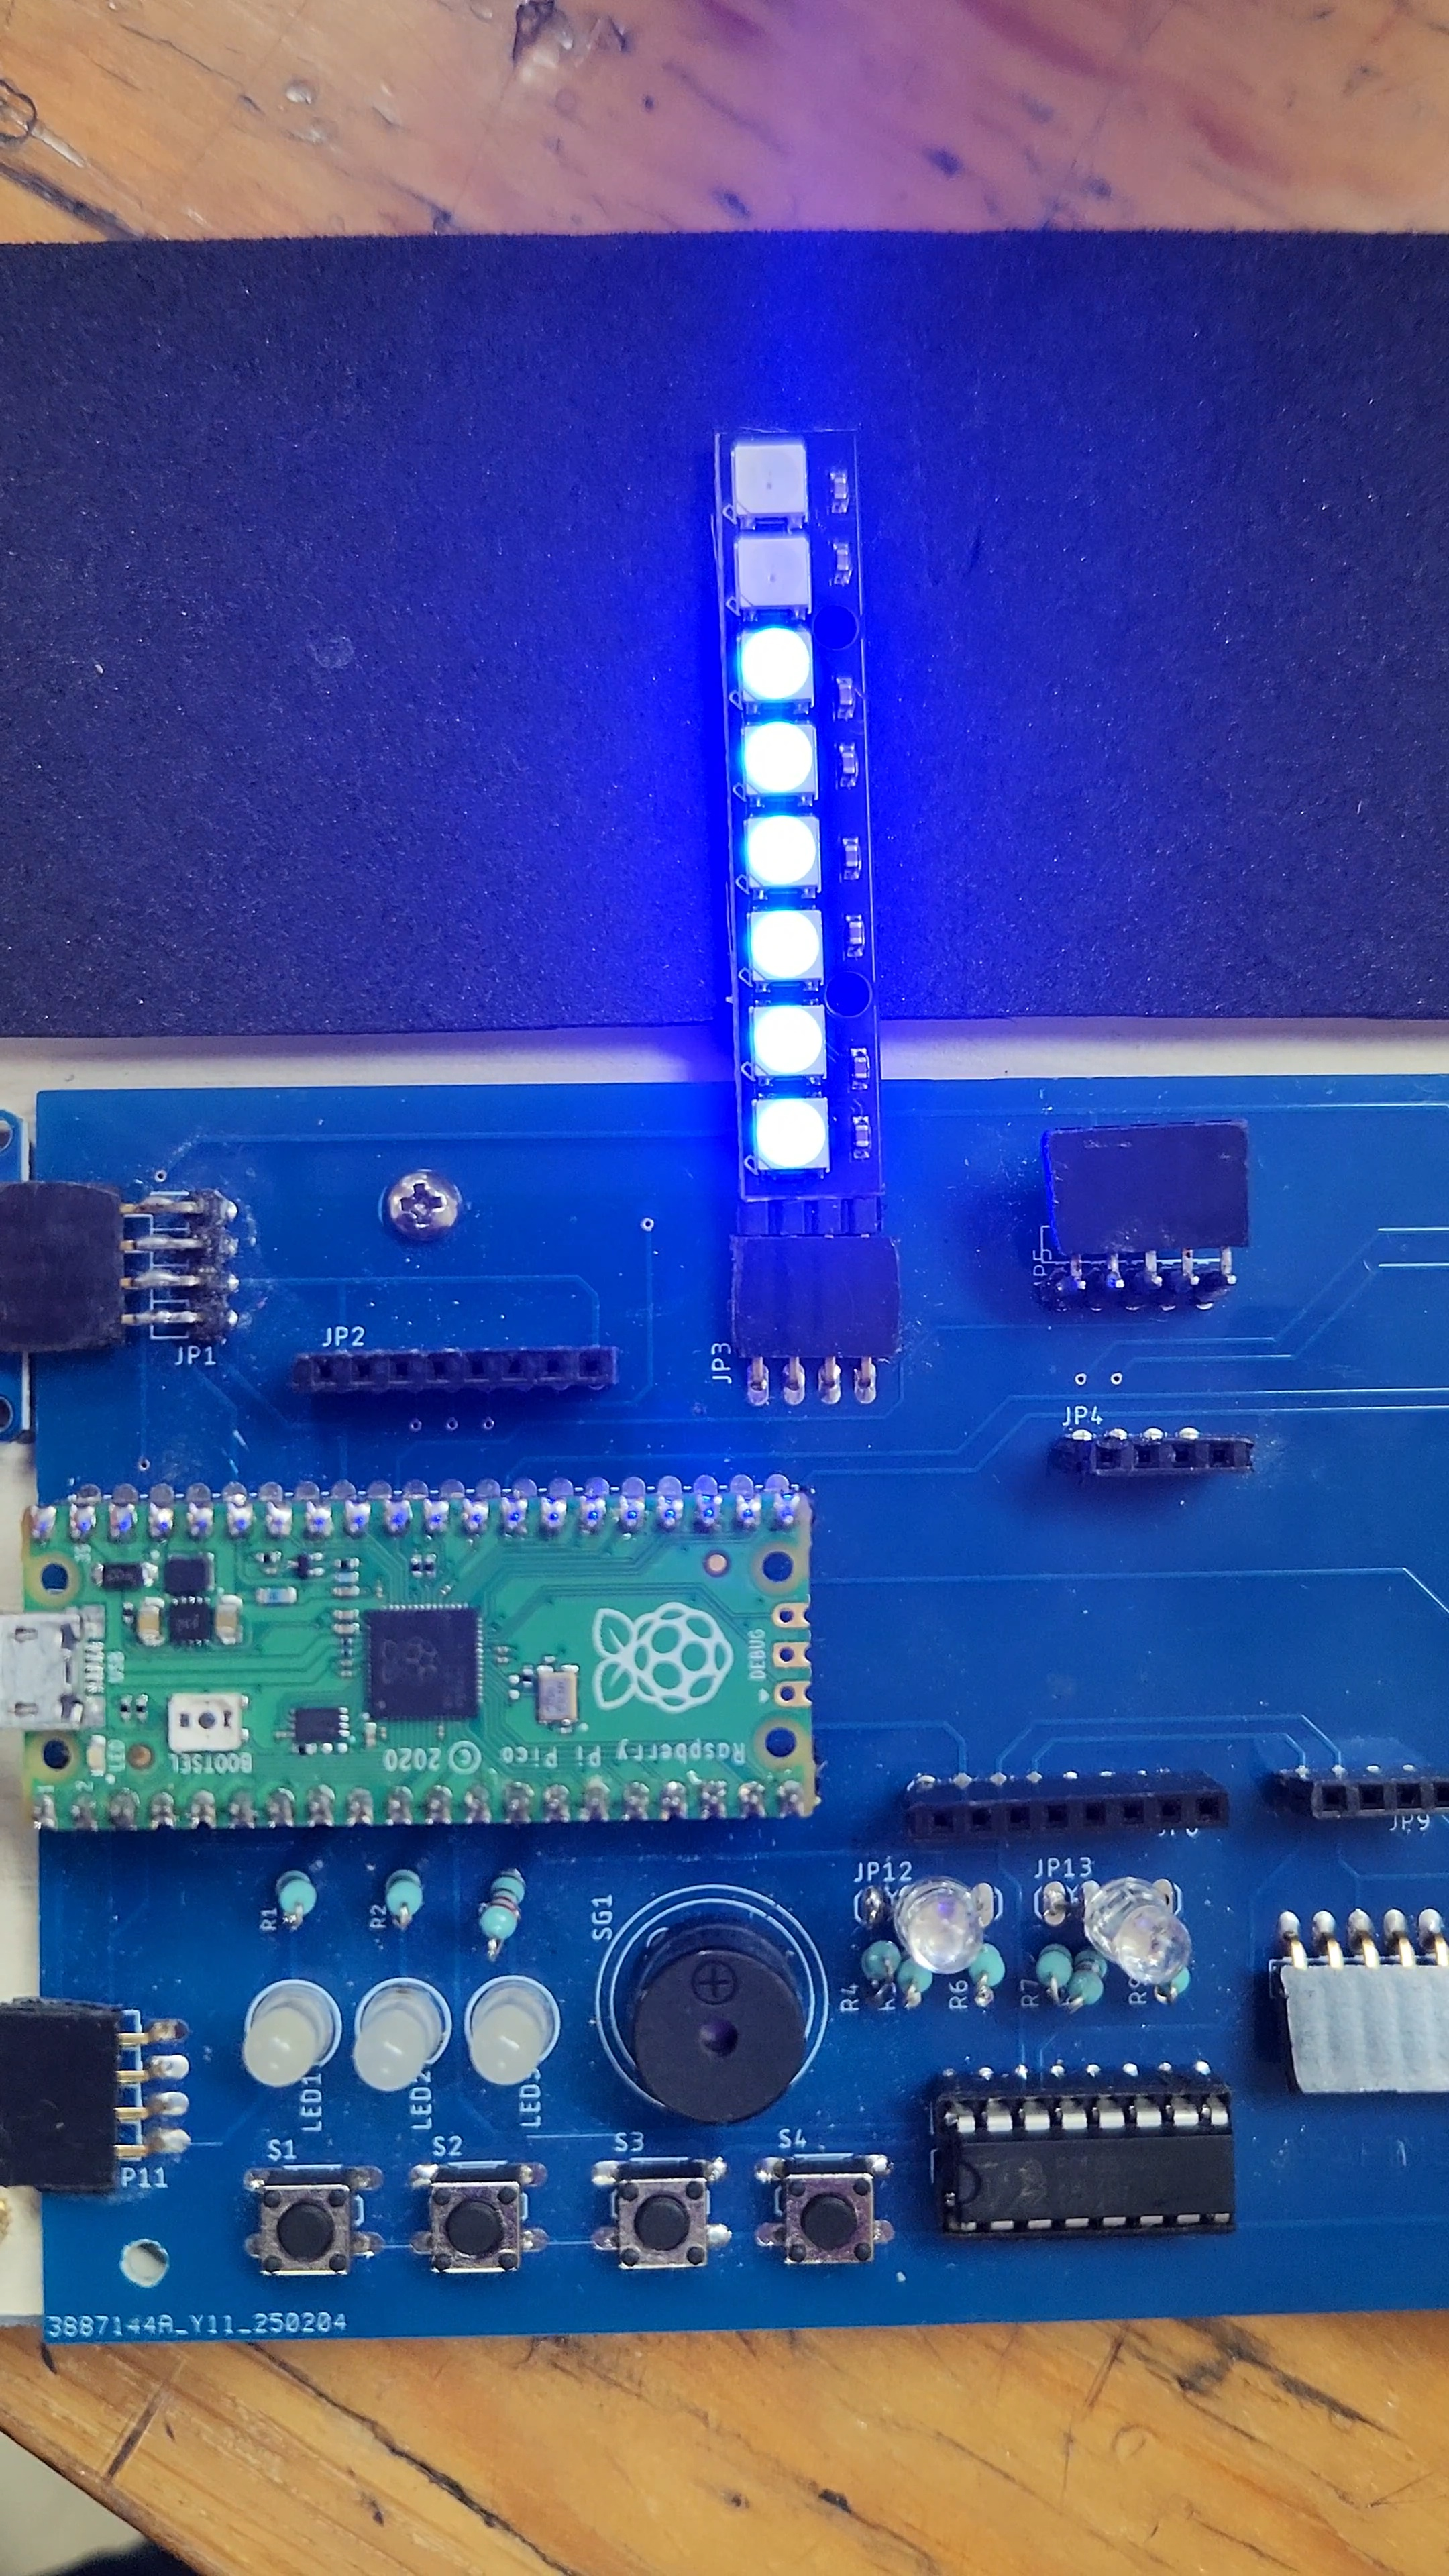
\includegraphics[width=\textwidth]{img/Actividad2/Act2_15.jpg}
        \caption{Posicion 6}
    \end{minipage}
\end{figure}

\begin{figure}[H]
    \centering
    \begin{minipage}{0.3\textwidth}
        \centering
        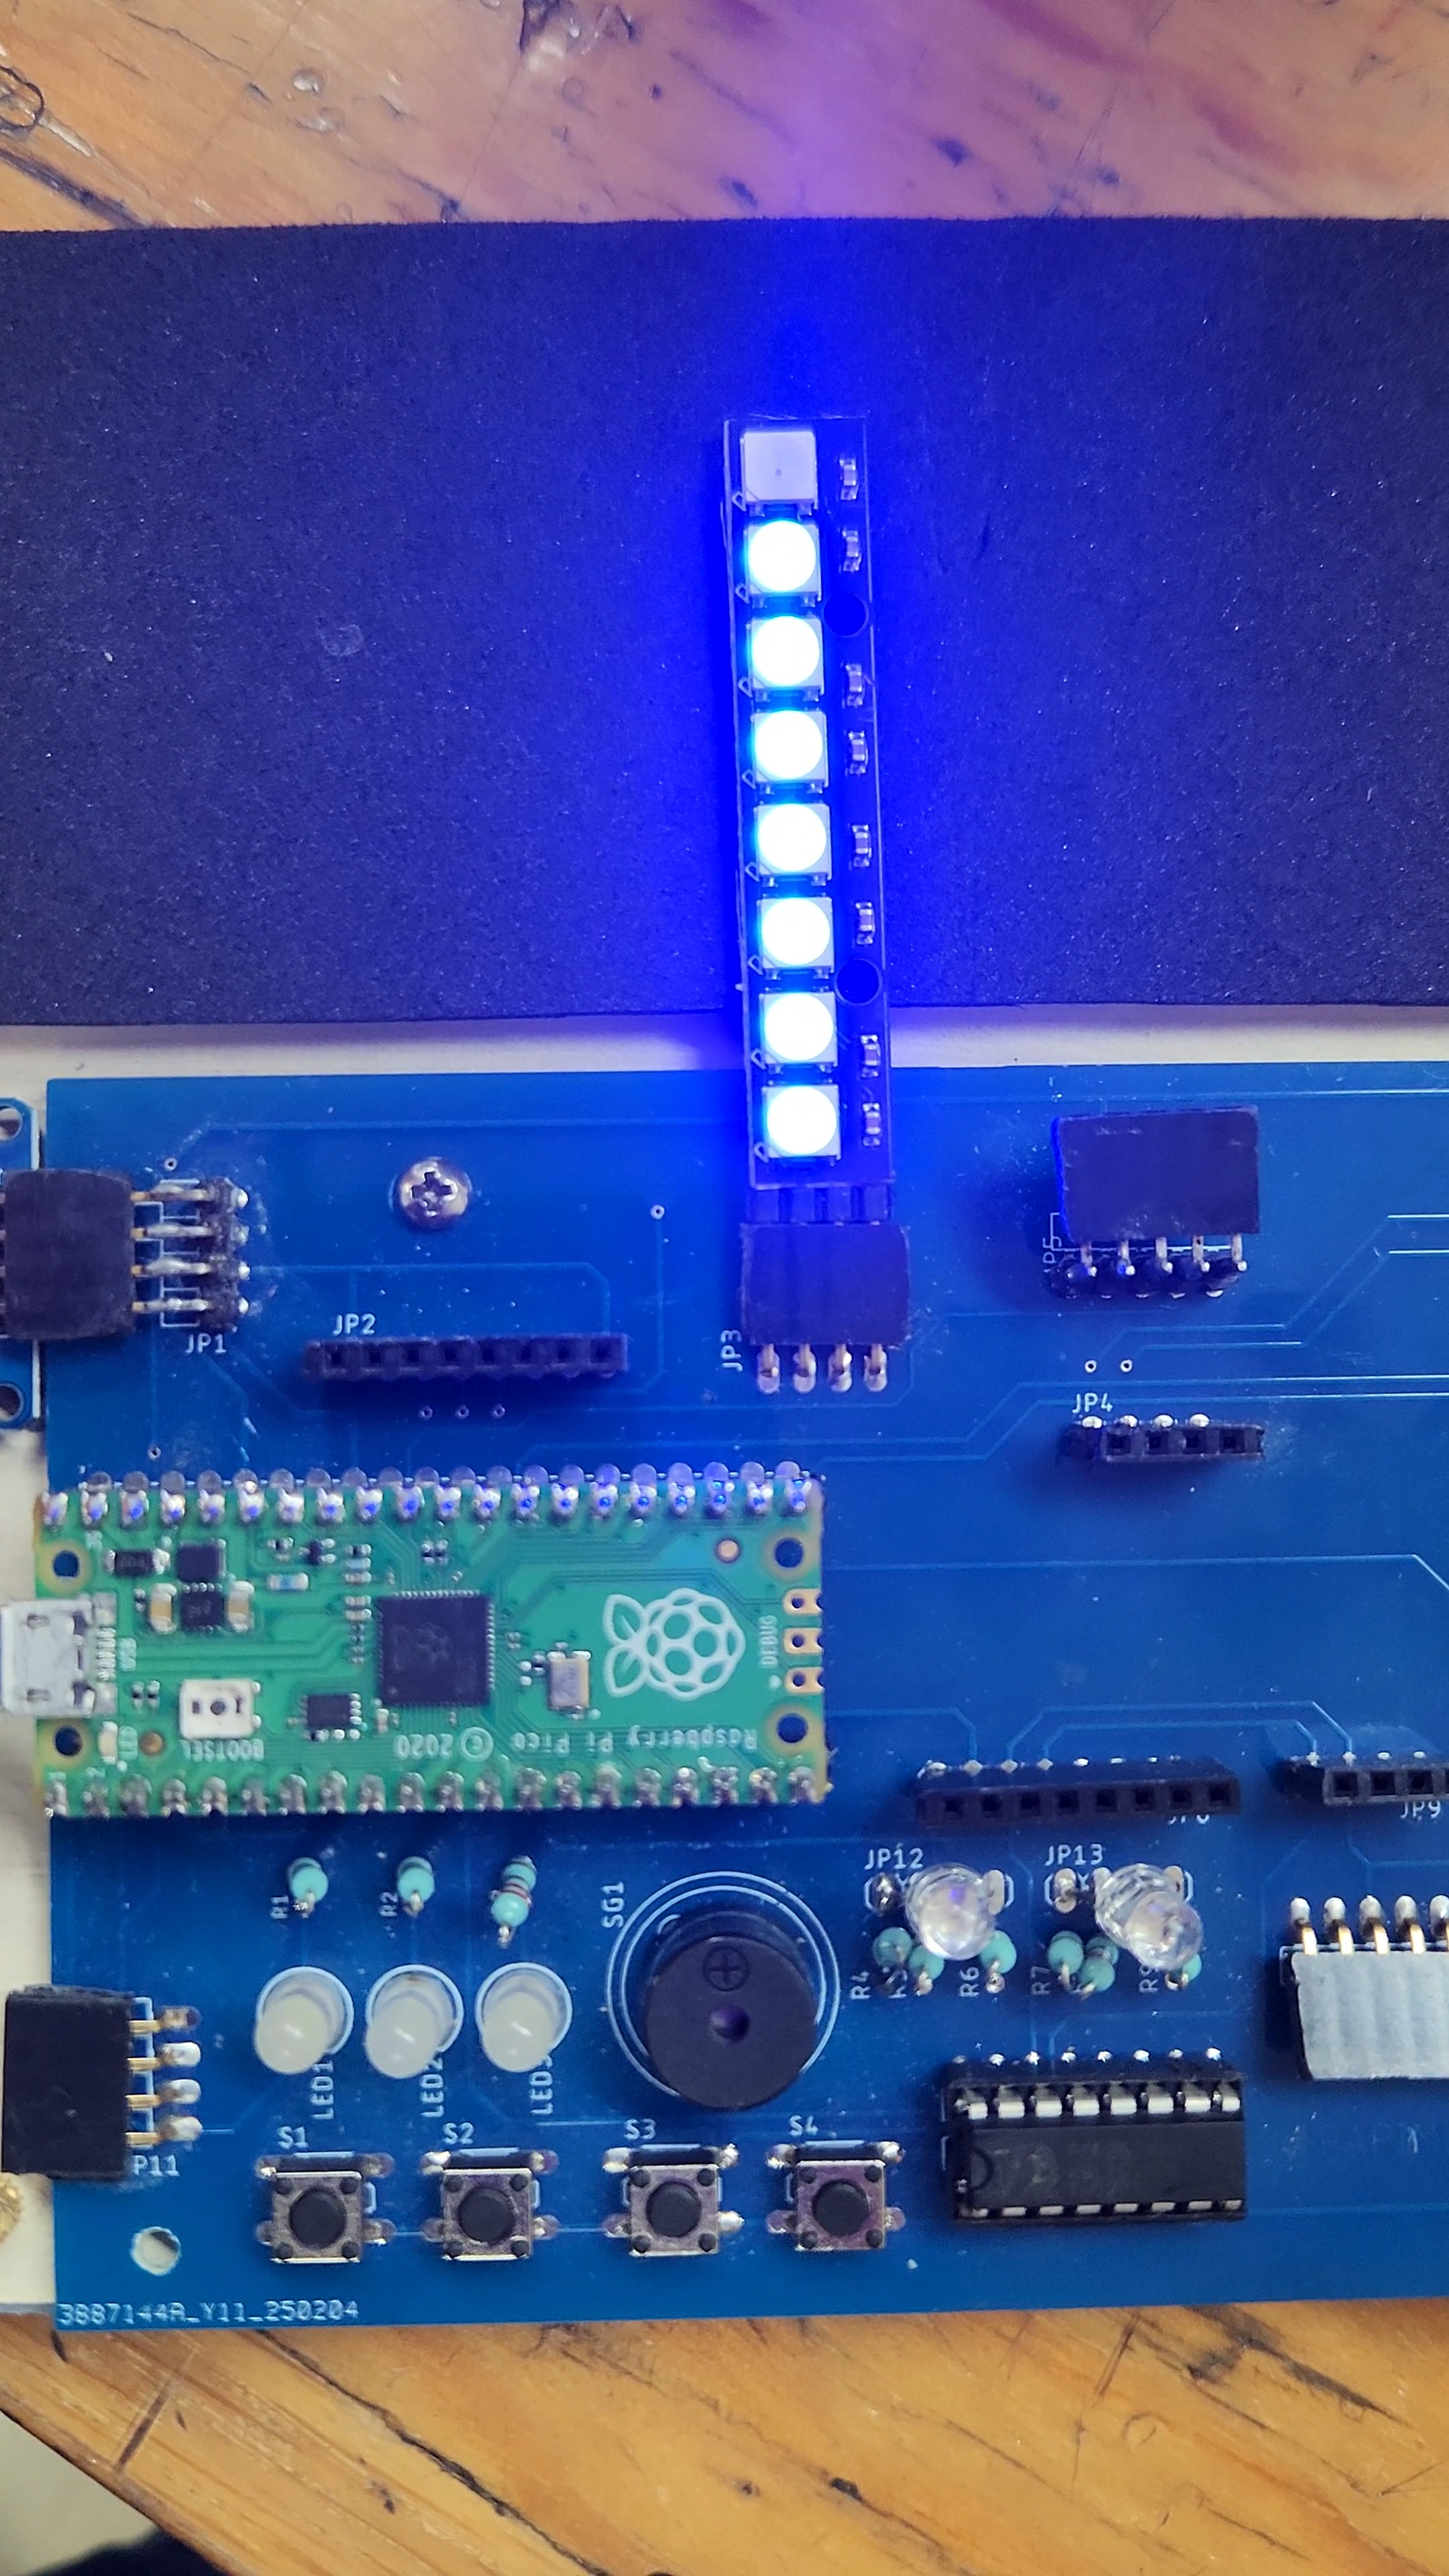
\includegraphics[width=\textwidth]{img/Actividad2/Act2_16.jpg}
        \caption{Posicion 9}
    \end{minipage}\hfill
    \begin{minipage}{0.3\textwidth}
        \centering
        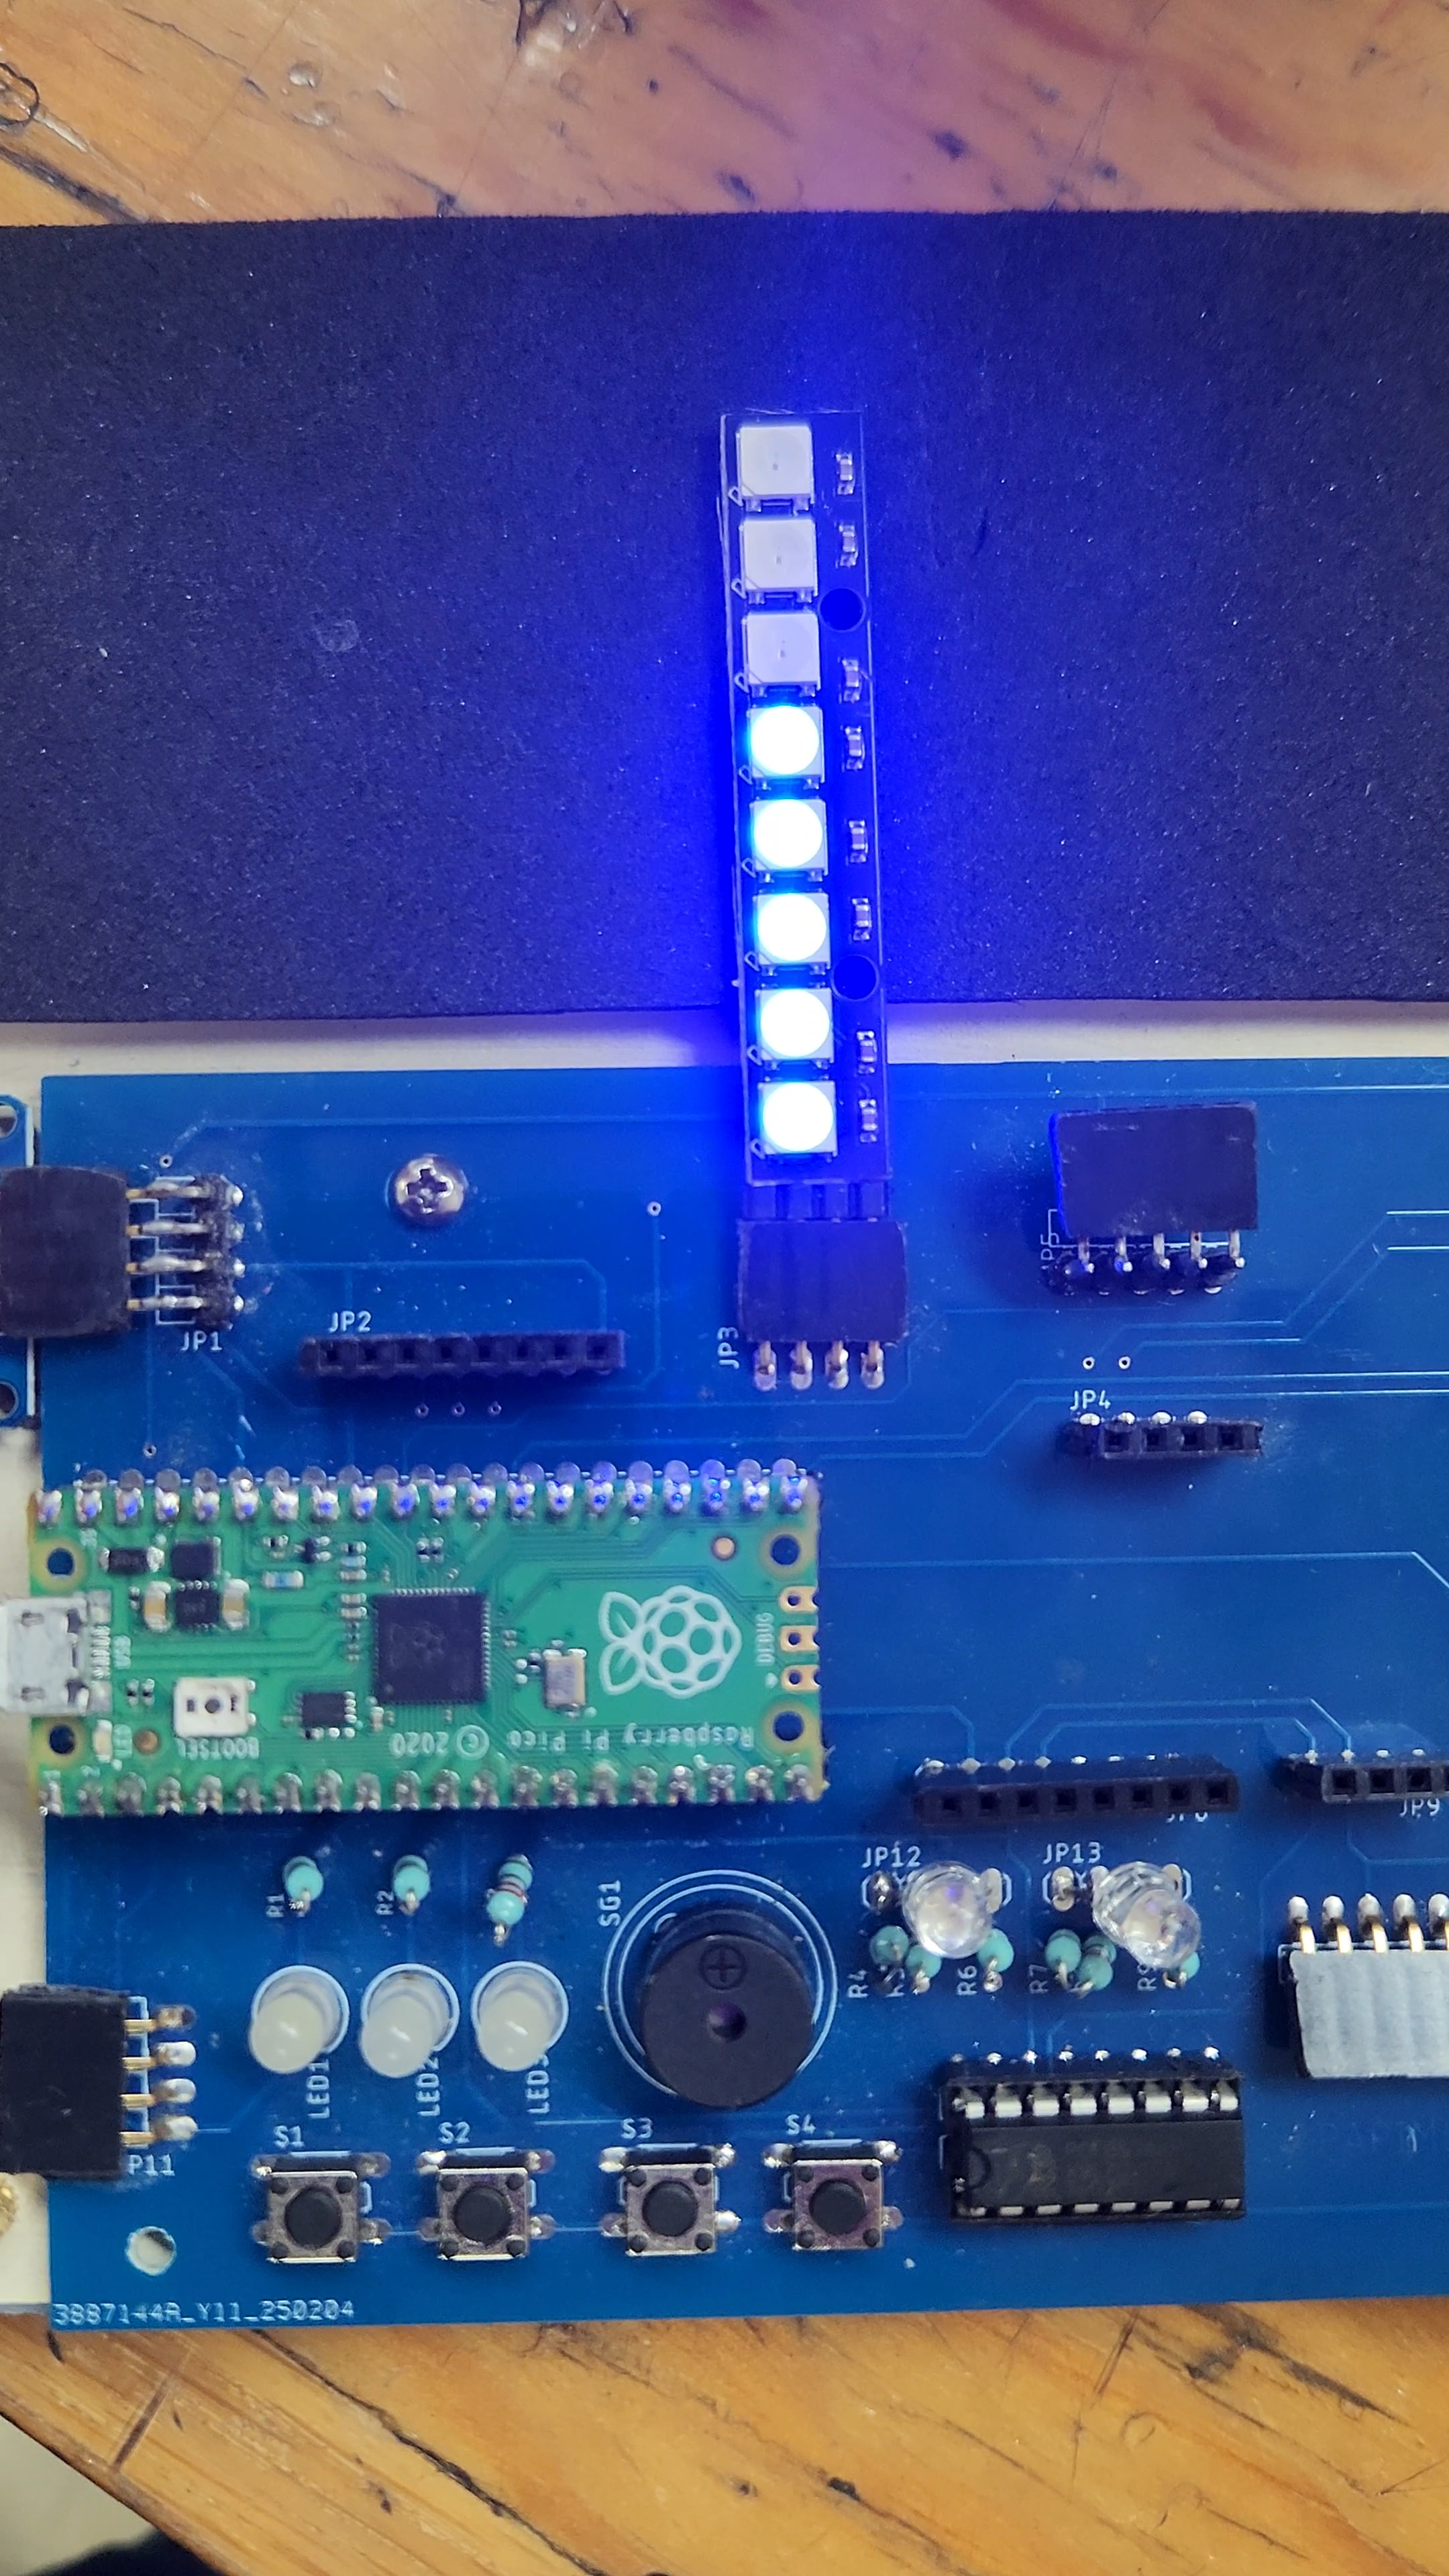
\includegraphics[width=\textwidth]{img/Actividad2/Act2_17.jpg}
        \caption{Posicion 11}
    \end{minipage}\hfill
    \begin{minipage}{0.3\textwidth}
        \centering
        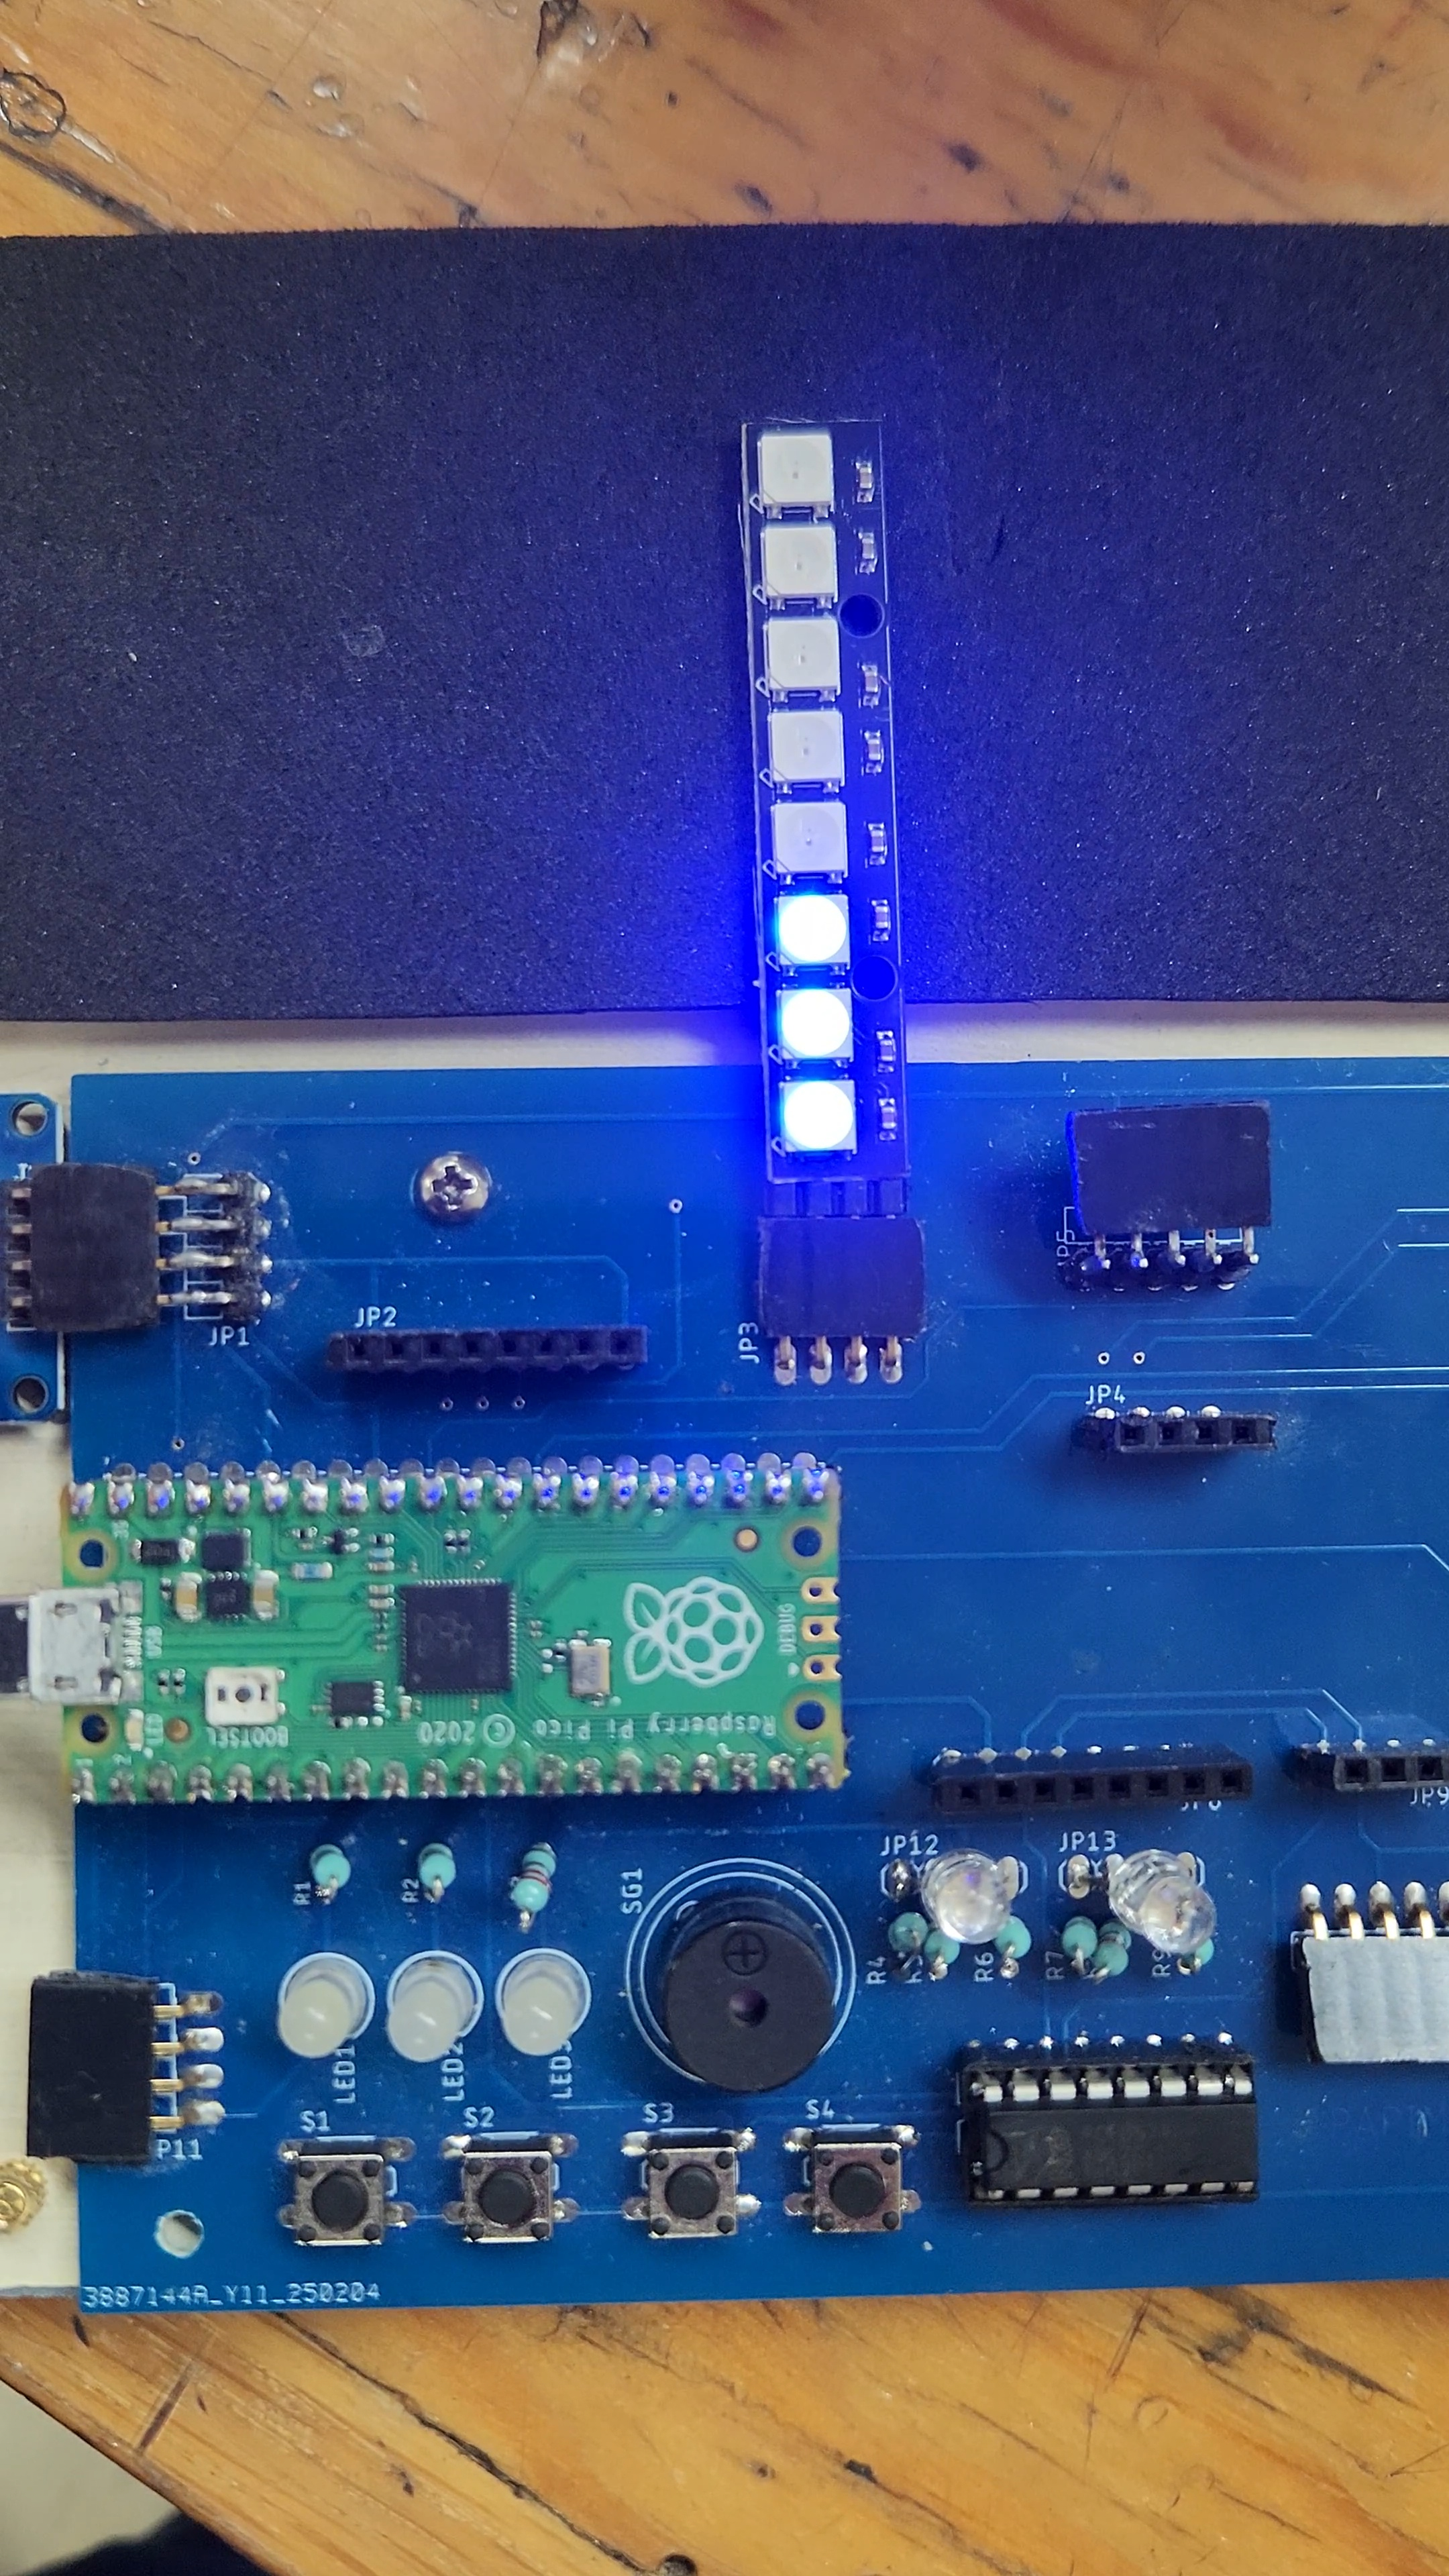
\includegraphics[width=\textwidth]{img/Actividad2/Act2_18.jpg}
        \caption{Posicion 13}
    \end{minipage}
\end{figure}

\begin{figure}[H]
    \centering
        \centering
        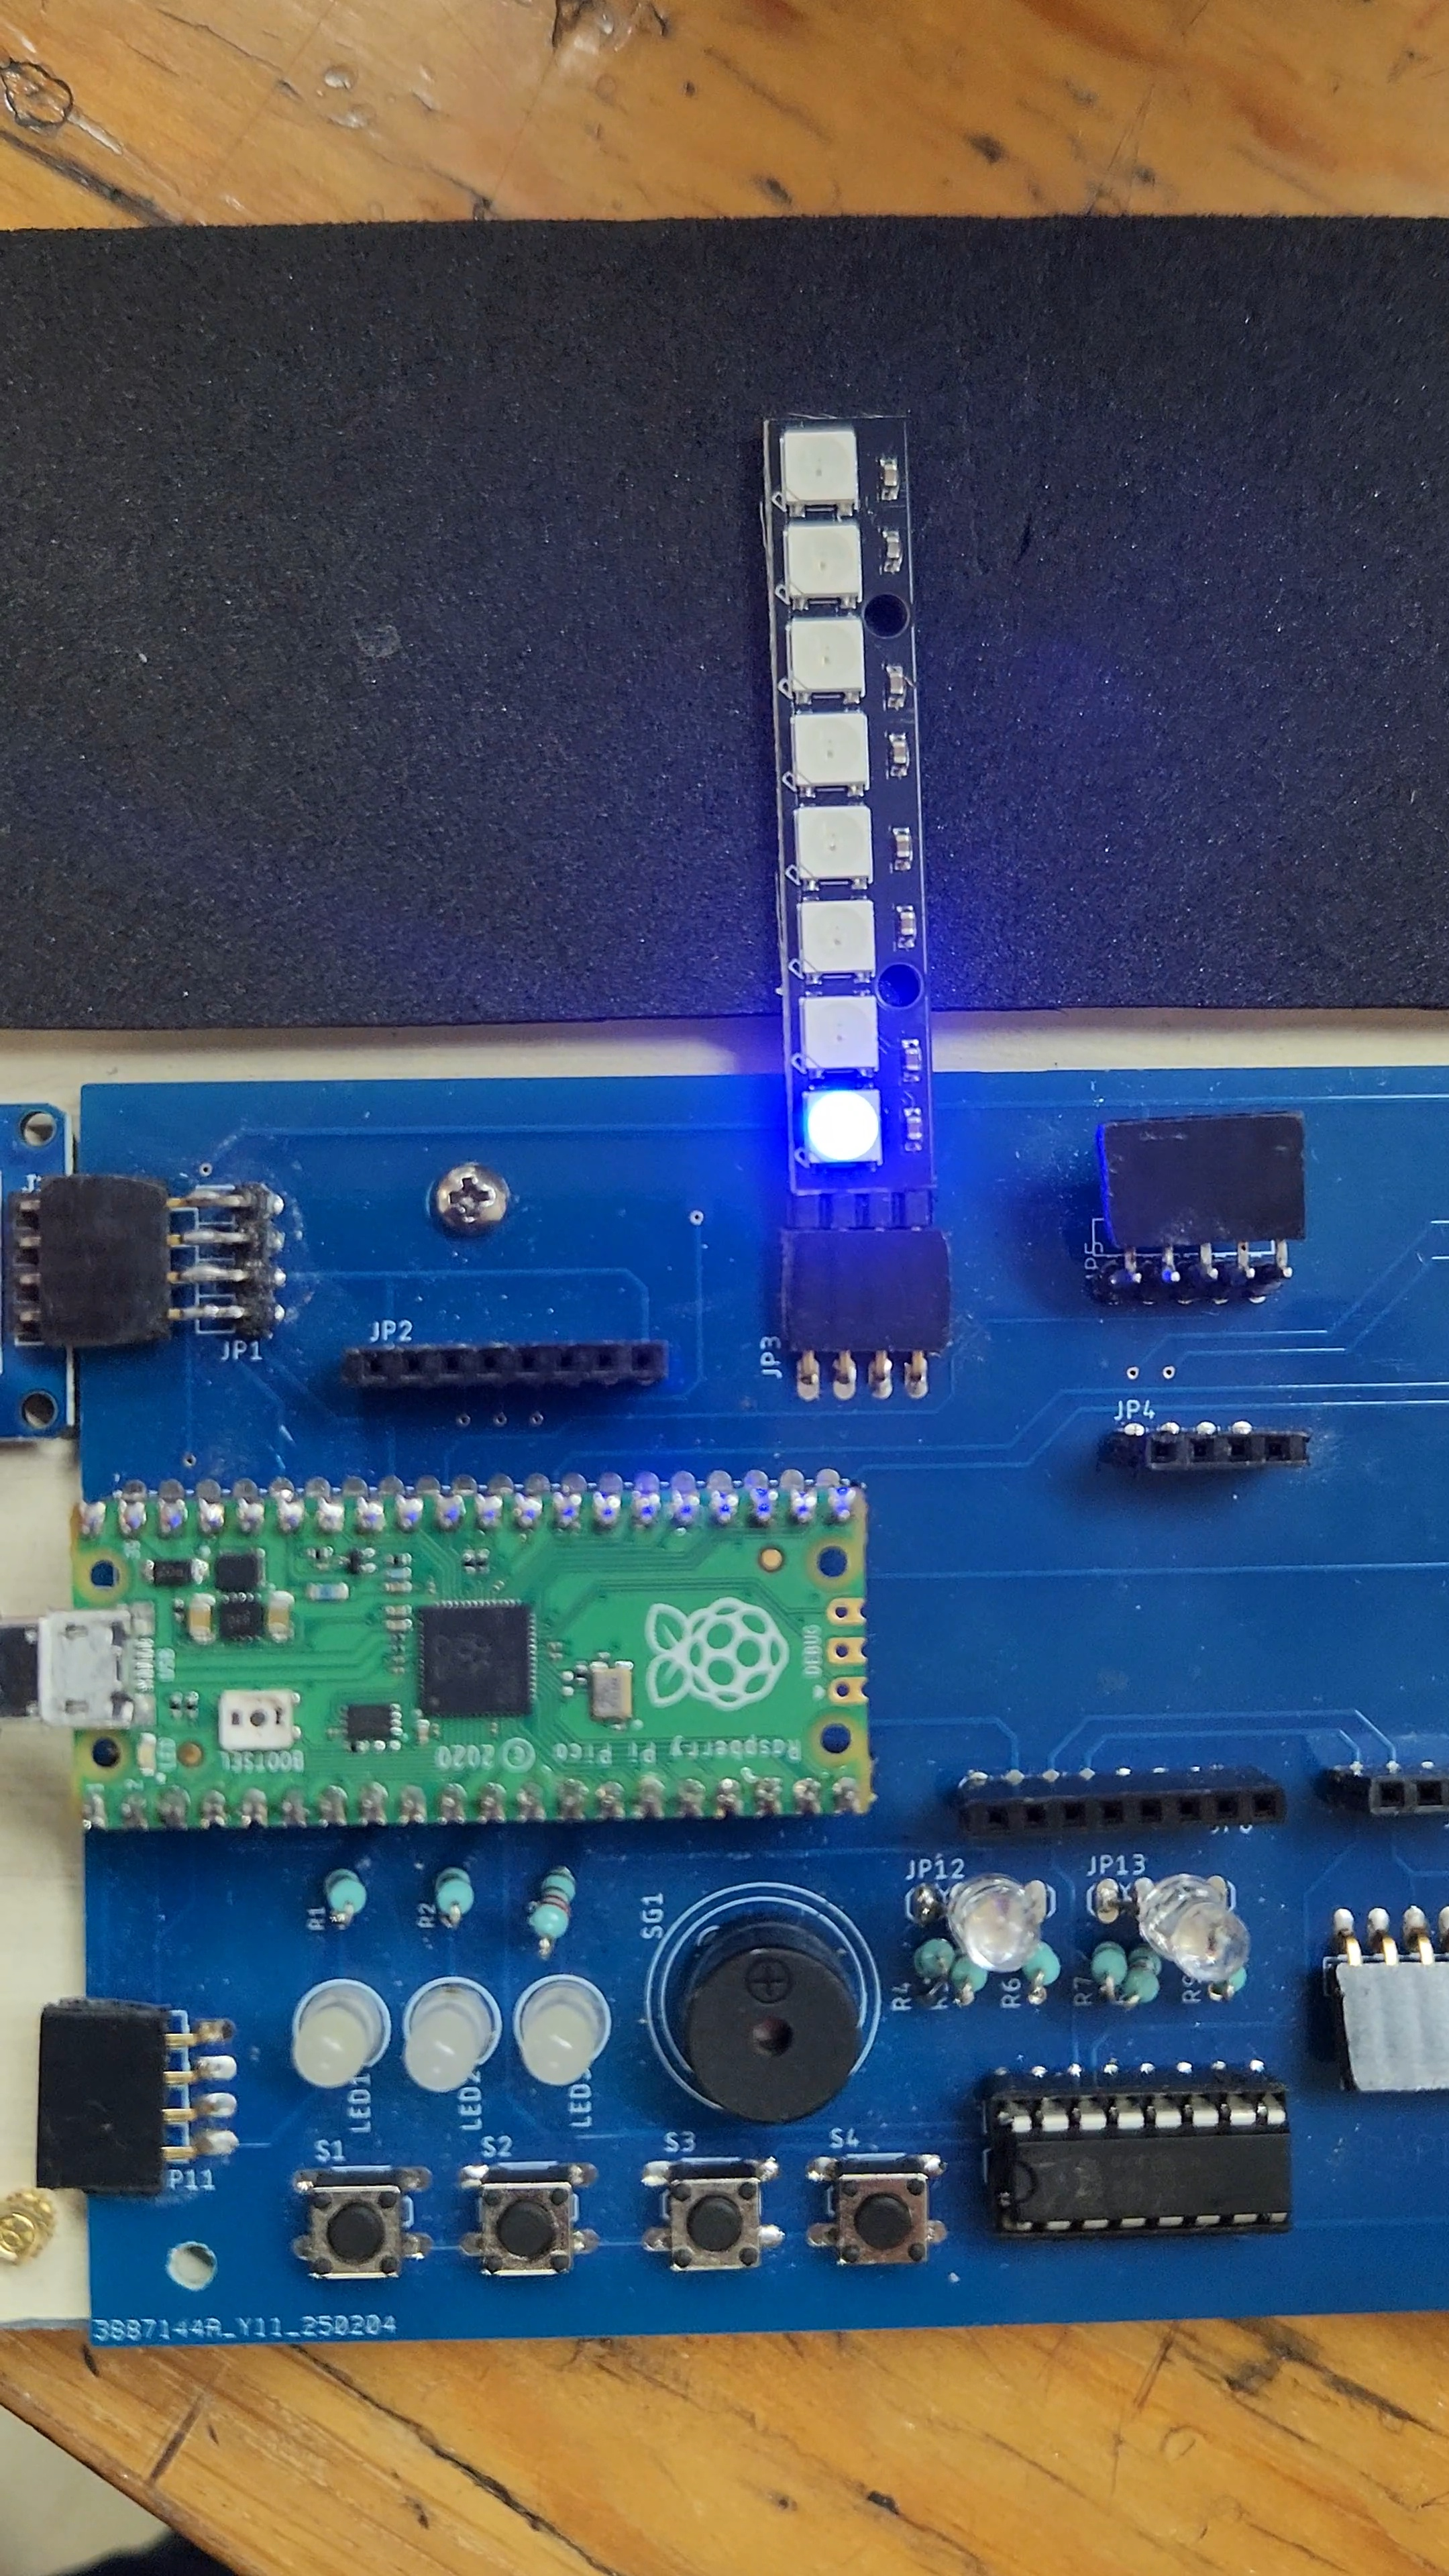
\includegraphics[width=0.3\textwidth]{img/Actividad2/Act2_19.jpg}
        \caption{Posicion 15}
\end{figure}

\subsection*{Analisis de resultados}

El programa ejecuta correctamente el efecto de barrido secuencial para los tres colores. El retardo de 0.5 segundos permite apreciar claramente cada transicion de encendido y apagado. El bucle ascendente (posiciones 0 a 7) genera un llenado progresivo de la tira, mientras que el bucle descendente (posiciones 7 a 0) vacia la tira. La eleccion de 0.5 segundos de retardo evita que el movimiento sea demasiado rapido para el ojo humano y las imagenes de la secuencia documentan cada posicion intermedia de la secuencia, validando el correcto funcionamiento del algoritmo.
    \newpage
    \section*{Actividad 3}

    \noindent Escribir, comentar e indicar el funcionamiento del siguiente programa; estudiar la librería usada.

    \vspace{1.5cm}

    % Diagrama
    \begin{center}
    \begin{tikzpicture}
        % 1. Dibujar la Raspberry Pi Pico
        \picoboard

        % 2. Dibujar el Display TM1637
        % Contorno principal del Display
        \draw[thick] (-6.5, 0.2) rectangle (-2.0, -1.3);
        
        % Título del Display
        \node[above, text=blue!80!black, font=\sffamily\itshape\large] at (-5.5, 0.3) {Display TM1637};
        
        % Los 4 dígitos (cuadrados interiores)
        \draw[thick] (-6.3, 0.0) rectangle (-5.4, -1.1);
        \draw[thick] (-5.2, 0.0) rectangle (-4.3, -1.1);
        \draw[thick] (-4.1, 0.0) rectangle (-3.2, -1.1);
        \draw[thick] (-3.0, 0.0) rectangle (-2.1, -1.1);

        % 3. Etiquetas de los pines del Display
        \node[right, font=\sffamily\bfseries\small] at (-2.0, 0.6) {VCC};
        \node[above left, font=\sffamily\bfseries\small] at (-0.8, -0.45) {CLK};
        \node[below left, font=\sffamily\bfseries\small] at (-0.8, -0.90) {DIO};
        \node[right, font=\sffamily\bfseries\small] at (-2.8, -1.6) {GND};

        % 4. Conexiones (Cables)
        
        % Cable CLK (Azul) a GP0 (y = -0.45)
        \draw[blue, thick] (-2.0, -0.45) -- (-0.4, -0.45);
        
        % Cable DIO (Verde) a GP1 (y = -0.90)
        \draw[green!70!black, thick] (-2.0, -0.90) -- (-0.4, -0.90);

        % Cable VCC (Rojo hacia arriba)
        \draw[red, thick] (-2.8, 0.2) -- (-2.8, 1.2);
        \node[above, font=\sffamily\footnotesize] at (-2.8, 1.2) {3.3V};
        % Base para la etiqueta 3.3V
        \draw[red, thick] (-3.0, 1.2) -- (-2.6, 1.2);

        % Cable GND (Negro hacia abajo con símbolo verde)
        \draw[black, thick] (-2.8, -1.3) -- (-2.8, -2.1);
        
        % Símbolo de GND (Líneas horizontales en verde)
        \draw[green!70!black, thick] (-3.2, -2.1) -- (-2.4, -2.1);
        \draw[green!70!black, thick] (-3.0, -2.3) -- (-2.6, -2.3);
        \draw[green!70!black, thick] (-2.85, -2.5) -- (-2.75, -2.5);

    \end{tikzpicture}
    \end{center}


    \section*{Propuesta de solución}
    Para implementar un reloj digital, se propone utilizar un módulo controlador de display de 7 segmentos TM1637. Este componente se comunica con el microcontrolador a través de un protocolo serie síncrono de dos hilos (CLK y DIO). La solución emplea la librería \texttt{tm1637} para abstraer el manejo a bajo nivel de los segmentos LED. 
    
    El programa plantea un bucle infinito que incrementa una variable de segundos, utilizando condicionales lógicas para manejar el acarreo matemático hacia los minutos cada vez que se alcanza el valor de 60. Para dar el efecto visual característico de un reloj real, se encienden y apagan los dos puntos centrales (\texttt{colon=True} y \texttt{colon=False}) intercalando retardos de medio segundo en el procesador. Esto logra una frecuencia de parpadeo estable de 1 Hz de manera sincronizada con el avance del tiempo.

    \begin{center}
        \scalebox{0.82}{
        \begin{tikzpicture}[node distance=1.05cm, every node/.style={font=\scriptsize}]
            \node (start3) [startstop, text width=2.8cm] {Inicio};
            \node (init3) [process, below=of start3, text width=7.2cm] {Inicializar \texttt{tm1637}, brillo, \texttt{Min=0} y \texttt{Sec=0}.};
            \node (on3) [process, below=of init3, text width=6.6cm] {Mostrar \texttt{Min:Sec} con \texttt{colon=True}, esperar 0.5 s.};
            \node (off3) [process, below=of on3, text width=6.6cm] {Mostrar \texttt{Min:Sec} con \texttt{colon=False}, esperar 0.5 s.};
            \node (incsec3) [process, below=of off3, text width=4.8cm] {\texttt{Sec = Sec + 1}.};
            \node (sec603) [decision, below=of incsec3, text width=3.2cm, aspect=2.2] {\texttt{Sec == 60}?};
            \node (incmin3) [process, below=of sec603, text width=5.4cm] {\texttt{Min = Min + 1}\newline \texttt{Sec = 0}};
            \node (min603) [decision, below=of incmin3, text width=3.2cm, aspect=2.2] {\texttt{Min == 60}?};
            \node (resetmin3) [process, below=of min603, text width=4.2cm] {\texttt{Min = 0}.};

            \draw [arrow] (start3) -- (init3);
            \draw [arrow] (init3) -- (on3);
            \draw [arrow] (on3) -- (off3);
            \draw [arrow] (off3) -- (incsec3);
            \draw [arrow] (incsec3) -- (sec603);
            \draw [arrow] (sec603) -- node[right, font=\scriptsize] {Si} (incmin3);
            \draw [arrow] (incmin3) -- (min603);
            \draw [arrow] (min603) -- node[right, font=\scriptsize] {Si} (resetmin3);
            
            % --- LÍNEAS CORREGIDAS ---
            % El texto "No" se coloca sobre la primera línea horizontal (node[above]).
            % Las distancias en X van de menor a mayor (1.5, 2.2, 2.9) para que no se crucen.
            % Las llegadas a `on3.east` tienen un yshift para entrar en alturas distintas.
            \draw [arrow] (sec603.east) -- node[above, font=\scriptsize] {No} ++(1.5,0) |- ([yshift=-0.25cm]on3.east);
            \draw [arrow] (min603.east) -- node[above, font=\scriptsize] {No} ++(2.2,0) |- (on3.east);
            \draw [arrow] (resetmin3.east) -- ++(2.9,0) |- ([yshift=0.25cm]on3.east);
            
        \end{tikzpicture}
        }
        \end{center}

    El flujo de datos inicia con la inicializacion del controlador TM1637 y de las variables \texttt{Min} y \texttt{Sec}. En cada iteracion se envian al display dos tramas consecutivas del mismo dato temporal (primero con dos puntos encendidos y luego apagados), despues se actualiza \texttt{Sec}. Cuando \texttt{Sec} alcanza 60, el flujo redirige el dato hacia \texttt{Min} y reinicia segundos; si \texttt{Min} llega a 60, tambien se reinicia. Finalmente, el valor normalizado vuelve al bloque de visualizacion y el ciclo se repite indefinidamente.

    \section*{Desarrollo}

    \lstinputlisting[language={[LAB]Python}, caption=Código de la Actividad 3, basicstyle=\ttfamily\scriptsize]{Code/Act3.py}
    

    \begin{figure}[H]
        \centering
        
\includegraphics[width=0.4\textwidth, angle=90]{img/Actividad3/Act3_1.jpg}
        \caption{Inicio de la ejecución (00:07). El microcontrolador inicializa la comunicación con el display TM1637. Las variables de minutos y segundos arrancan en cero, y la instrucción \texttt{tm.numbers(Min, Sec, colon=True)} enciende de manera estática los dos puntos centrales.}
    \end{figure}

    \begin{figure}[H]
        \centering
        
\includegraphics[width=0.4\textwidth, angle=90]{img/Actividad3/Act3_2.jpg}
        \caption{Efecto de parpadeo inicial. Tras un retardo de 500 ms, el programa actualiza la pantalla pasando el parámetro \texttt{colon=False}, lo que apaga los LEDs centrales simulando el pulso visual característico de un segundero real.}
    \end{figure}

    \begin{figure}[H]
        \centering
        
\includegraphics[width=0.4\textwidth, angle=90]{img/Actividad3/Act3_3.jpg}
        \caption{Avance continuo del reloj (00:09). La lógica del bucle incrementa la variable \texttt{Sec}. El protocolo serie sincroniza los registros de los cuatro dígitos del módulo simultáneamente para reflejar el progreso del tiempo con el separador activo.}
    \end{figure}

    \begin{figure}[H]
        \centering
        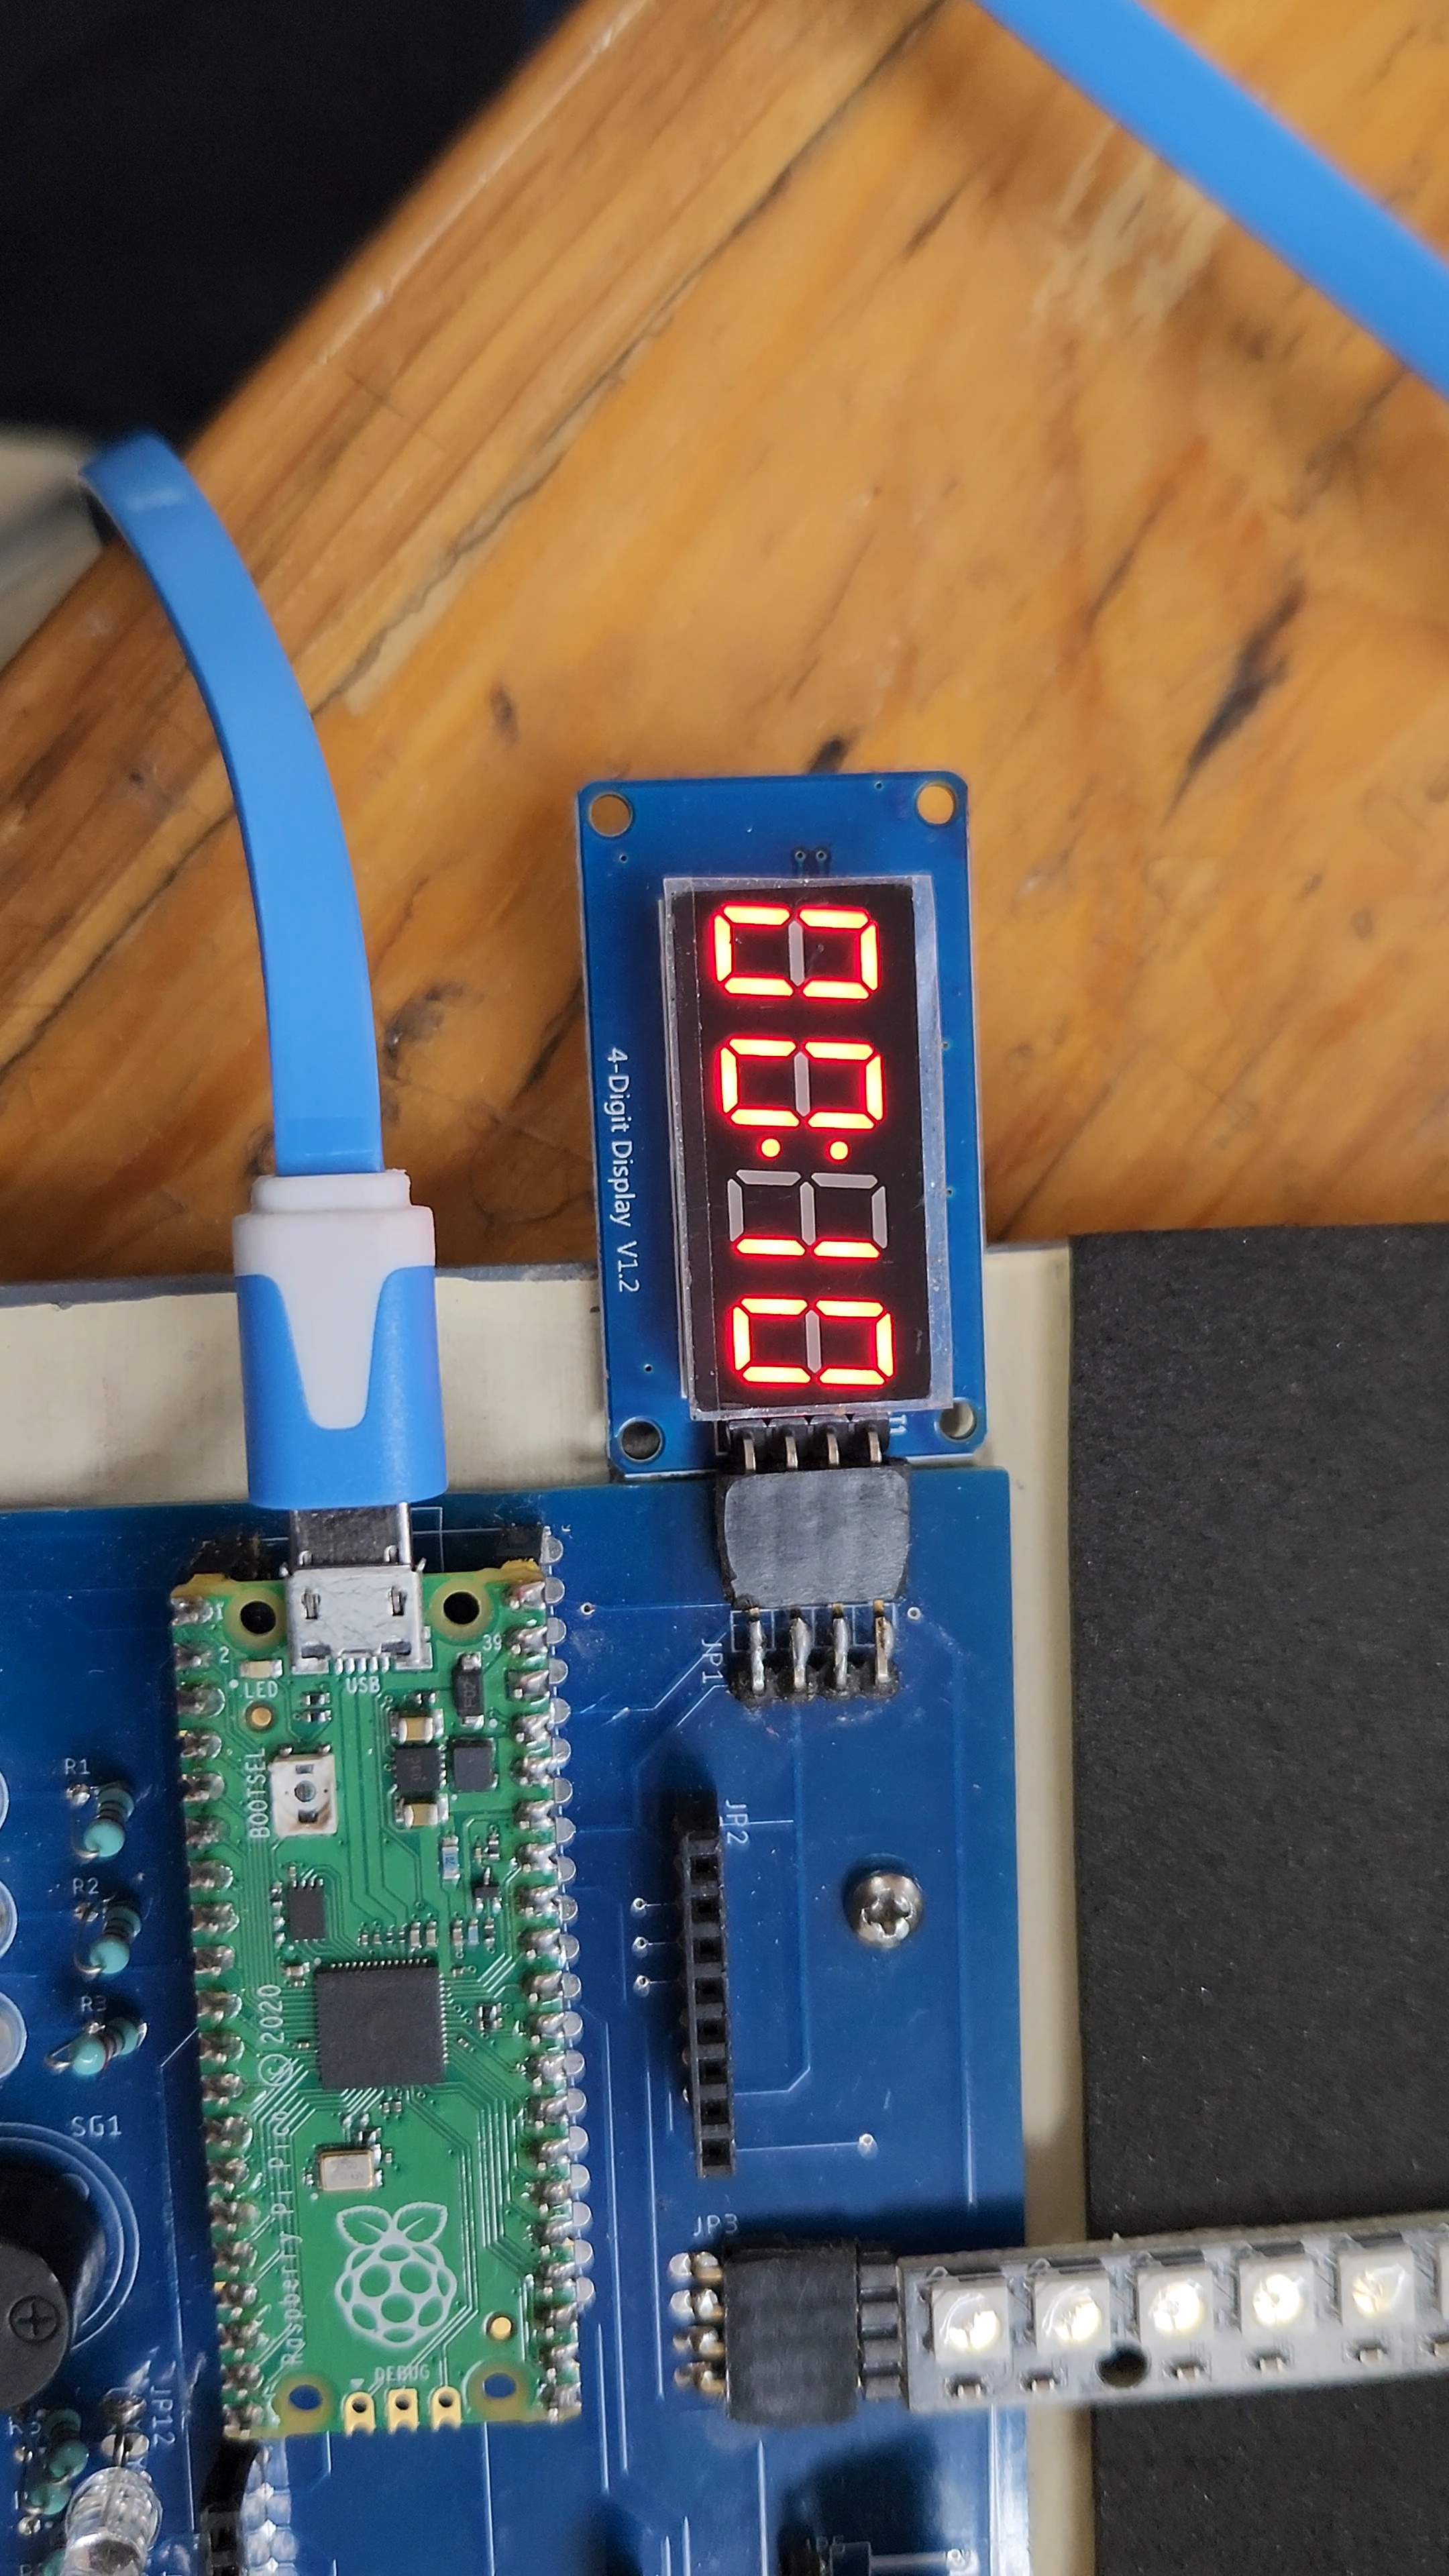
\includegraphics[width=0.4\textwidth, angle=90]{img/Actividad3/Act3_4.jpg}
        \caption{Avance continuo del reloj (00:10).}
    \end{figure}

    \begin{figure}[H]
        \centering
        
\includegraphics[width=0.4\textwidth, angle=90]{img/Actividad3/Act3_5.jpg}
        \caption{Avance continuo del reloj (00:11).}
    \end{figure}

    \begin{figure}[H]
        \centering
        
\includegraphics[width=0.4\textwidth, angle=90]{img/Actividad3/Act3_6.jpg}
        \caption{Culminación del ciclo de muestra. }
    \end{figure}


    \subsection*{Análisis de resultados}
    Al ejecutar el programa, se comprueba la comunicación exitosa entre el RP2040 y el circuito integrado TM1637. La instrucción \texttt{tm.numbers(Min, Sec)} procesa internamente las variables enteras y envía la trama de datos necesaria para encender los LEDs correctos en los cuatro dígitos de manera simultánea, evitando la necesidad de hacer multiplexación manual por software.

    El efecto de segundero se logra dividiendo el retardo total de un segundo en dos pausas de 0.5 segundos. En la primera mitad, el microcontrolador envía los datos con el parámetro de los dos puntos activado, y en la segunda mitad envía la instrucción de apagado. Las estructuras condicionales \texttt{if Sec == 60} y \texttt{if Min == 60} gestionan el reinicio de las variables, asegurando que el formato de reloj base 60 se mantenga íntegro ciclo tras ciclo antes de realizar la siguiente escritura en la pantalla.
    \newpage

\section*{Actividad 4}

\noindent Empleando el display TM1637; realizar un programa que muestre un contador descendente, iniciando en 20 y cuando corresponda el valor 0, active un sonido de 1 segundo de duracion en el zumbador de la tarjeta (GPIO17).

\vspace{1.5cm}

% Diagrama
\begin{center}
\begin{tikzpicture}
    % 1. Dibujar la Raspberry Pi Pico
    \picoboard

    % ==========================================
    % 2. Modulo Display TM1637 (Lado Izquierdo)
    % ==========================================
    
    % Contorno principal del Display
    \draw[thick] (-6.5, 0.2) rectangle (-2.0, -1.3);
    
    % Titulo del Display
    \node[above, text=blue!80!black, font=\sffamily\itshape\large] at (-5.5, 0.3) {Display TM1637};
    
    % Los 4 digitos
    \draw[thick] (-6.3, 0.0) rectangle (-5.4, -1.1);
    \draw[thick] (-5.2, 0.0) rectangle (-4.3, -1.1);
    \draw[thick] (-4.1, 0.0) rectangle (-3.2, -1.1);
    \draw[thick] (-3.0, 0.0) rectangle (-2.1, -1.1);

    % Cables del Display
    % Cable CLK (Azul) a GP0
    \draw[blue, thick] (-2.0, -0.45) -- (-0.4, -0.45);
    \node[above, font=\sffamily\bfseries\small, inner sep=2pt] at (-1.5, -0.45) {CLK};
    
    % Cable DIO (Verde) a GP1
    \draw[green!70!black, thick] (-2.0, -0.90) -- (-0.4, -0.90);
    \node[below, font=\sffamily\bfseries\small, inner sep=2pt] at (-1.5, -0.90) {DIO};

    % Cable VCC (Rojo hacia arriba)
    \draw[red, thick] (-2.8, 0.2) -- (-2.8, 1.2);
    \node[right, font=\sffamily\bfseries\small, inner sep=4pt] at (-2.8, 0.6) {VCC};
    \node[above, font=\sffamily\footnotesize] at (-2.8, 1.2) {3.3V};
    \draw[red, thick] (-3.0, 1.2) -- (-2.6, 1.2);

    % Cable GND (Negro hacia abajo)
    \draw[black, thick] (-2.8, -1.3) -- (-2.8, -2.1);
    \node[right, font=\sffamily\bfseries\small, inner sep=4pt] at (-2.8, -1.7) {GND};
    
    % Simbolo de GND
    \draw[green!70!black, thick] (-3.2, -2.1) -- (-2.4, -2.1);
    \draw[green!70!black, thick] (-3.0, -2.3) -- (-2.6, -2.3);
    \draw[green!70!black, thick] (-2.85, -2.5) -- (-2.75, -2.5);

    % ==========================================
    % 3. Modulo Zumbador (Lado Derecho)
    % ==========================================
    
    % Conexion del zumbador al pin GP17
    \draw[red, thick] (4.4, -8.55) -- (5.2, -8.55);
    
    % Dibujo del Zumbador
    \draw[thick, fill=white] (5.2, -8.2) rectangle (5.5, -8.9);
    \draw[thick, fill=white] (5.5, -8.2) -- (6.0, -7.9) -- (6.0, -9.2) -- (5.5, -8.9) -- cycle;

    % Cable GND del Zumbador
    \draw[black, thick] (5.35, -8.9) -- (5.35, -9.6);
    
    % Simbolo de GND
    \draw[green!70!black, thick] (4.95, -9.6) -- (5.75, -9.6);
    \draw[green!70!black, thick] (5.15, -9.8) -- (5.55, -9.8);
    \draw[green!70!black, thick] (5.3, -10.0) -- (5.4, -10.0);

\end{tikzpicture}

\vspace{0.8cm}
{\sffamily Figura 9-13. Esquematico de la actividad 4}
\end{center}

\section*{Propuesta de solucion}

Se emplea el modulo TM1637 para controlar un display de 4 digitos de 7 segmentos mediante los pines GPIO 0 (CLK) y GPIO 1 (DIO), utilizando la libreria \texttt{tm1637}. El zumbador pasivo se conecta al GPIO 17 como salida digital. El algoritmo implementa un contador descendente desde 20 hasta 0 usando el metodo \texttt{number()} del display para mostrar el valor actual. En cada iteracion se aplica una pausa de 1 segundo y al alcanzar el valor 0, el programa pone el pin del zumbador en nivel alto durante 1 segundo para generar un tono audible, y luego lo apaga.

% Diagrama de flujo
\begin{center}
    \scalebox{0.85}{
    \begin{tikzpicture}[node distance=1.05cm, every node/.style={font=\scriptsize}]
        \node (start4) [startstop, text width=2.6cm] {Inicio};
        \node (init4) [process, below=of start4, text width=8.2cm] {Importar librerias. Configurar TM1637 en GPIO 0 y 1, brillo 3. Configurar zumbador en GPIO 17 como salida.};
        \node (for4) [process, below=of init4, text width=5.5cm] {\texttt{for cuenta in range(20, -1, -1)}:};
        \node (show4) [process, below=of for4, text width=5.2cm] {Mostrar \texttt{cuenta} en display con \texttt{tm.number(cuenta)}.};
        \node (wait4) [process, below=of show4, text width=4.2cm] {Esperar 1 segundo con \texttt{sleep(1)}.};
        \node (check4) [decision, below=of wait4, text width=3.5cm, aspect=2.2] {\texttt{cuenta == 0}?};
        \node (alarm4) [process, below=of check4, text width=6.2cm] {Activar zumbador: \texttt{zumbador.value(1)}. Esperar 1 segundo. Apagar zumbador: \texttt{zumbador.value(0)}.};
        \node (end4) [startstop, below=of alarm4, text width=2.2cm] {Fin};
        
        \draw [arrow] (start4) -- (init4);
        \draw [arrow] (init4) -- (for4);
        \draw [arrow] (for4) -- (show4);
        \draw [arrow] (show4) -- (wait4);
        \draw [arrow] (wait4) -- (check4);
        
        % Flecha "No" (aun no es cero) - regresa al siguiente valor del for
        \draw [arrow] (check4.east) -- node[above, font=\scriptsize] {No} ++(1.8,0) |- ([yshift=-0.3cm]for4.east);
        
        % Flecha "Si" (llegó a cero)
        \draw [arrow] (check4.south) -- node[right, font=\scriptsize] {Si} (alarm4);
        
        % Flecha de alarm4 hacia Fin
        \draw [arrow] (alarm4) -- (end4);
        
    \end{tikzpicture}
    }
\end{center}

\section*{Desarrollo}

\lstinputlisting[language={[LAB]Python}, caption=Codigo de la Actividad 4, basicstyle=\ttfamily\scriptsize]{Code/Act4.py}

\begin{figure}[H]
    \centering
    \begin{minipage}{0.3\textwidth}
        \centering
        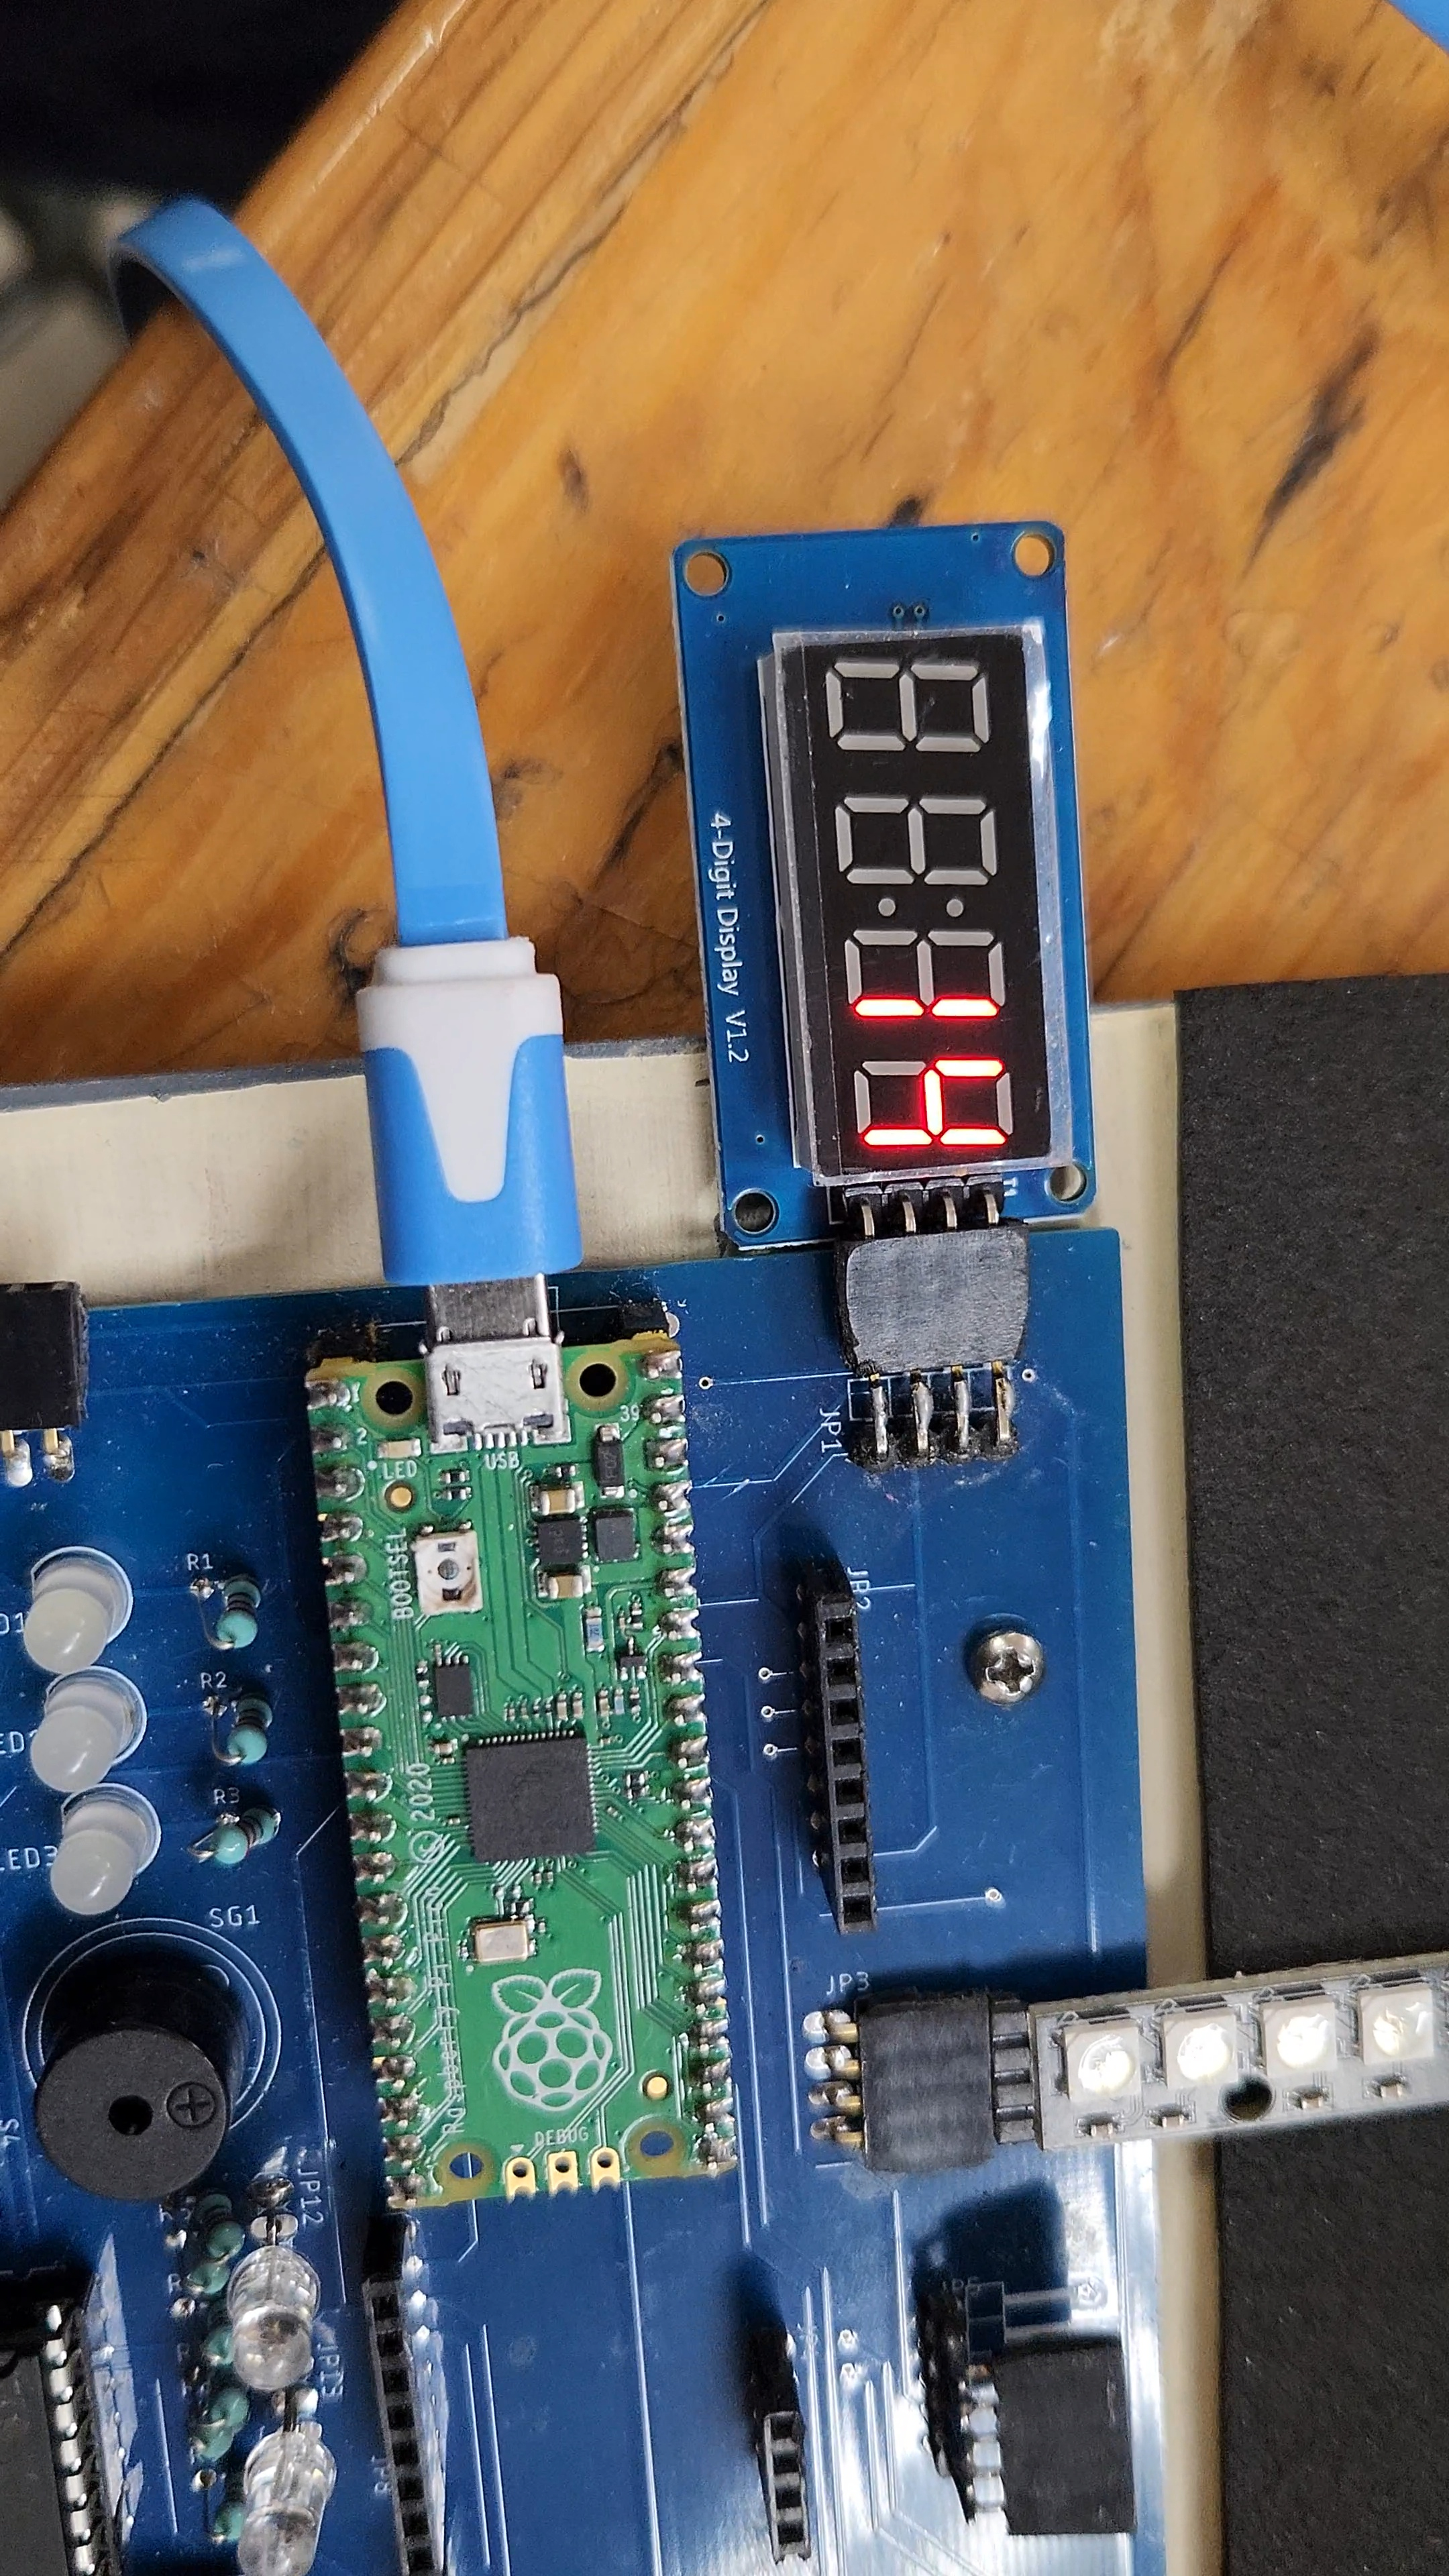
\includegraphics[width=0.6\textwidth, angle=90]{img/Actividad4/Act4_15.jpg}
        \caption{Valor 20}
    \end{minipage}
    \begin{minipage}{0.3\textwidth}
        \centering
        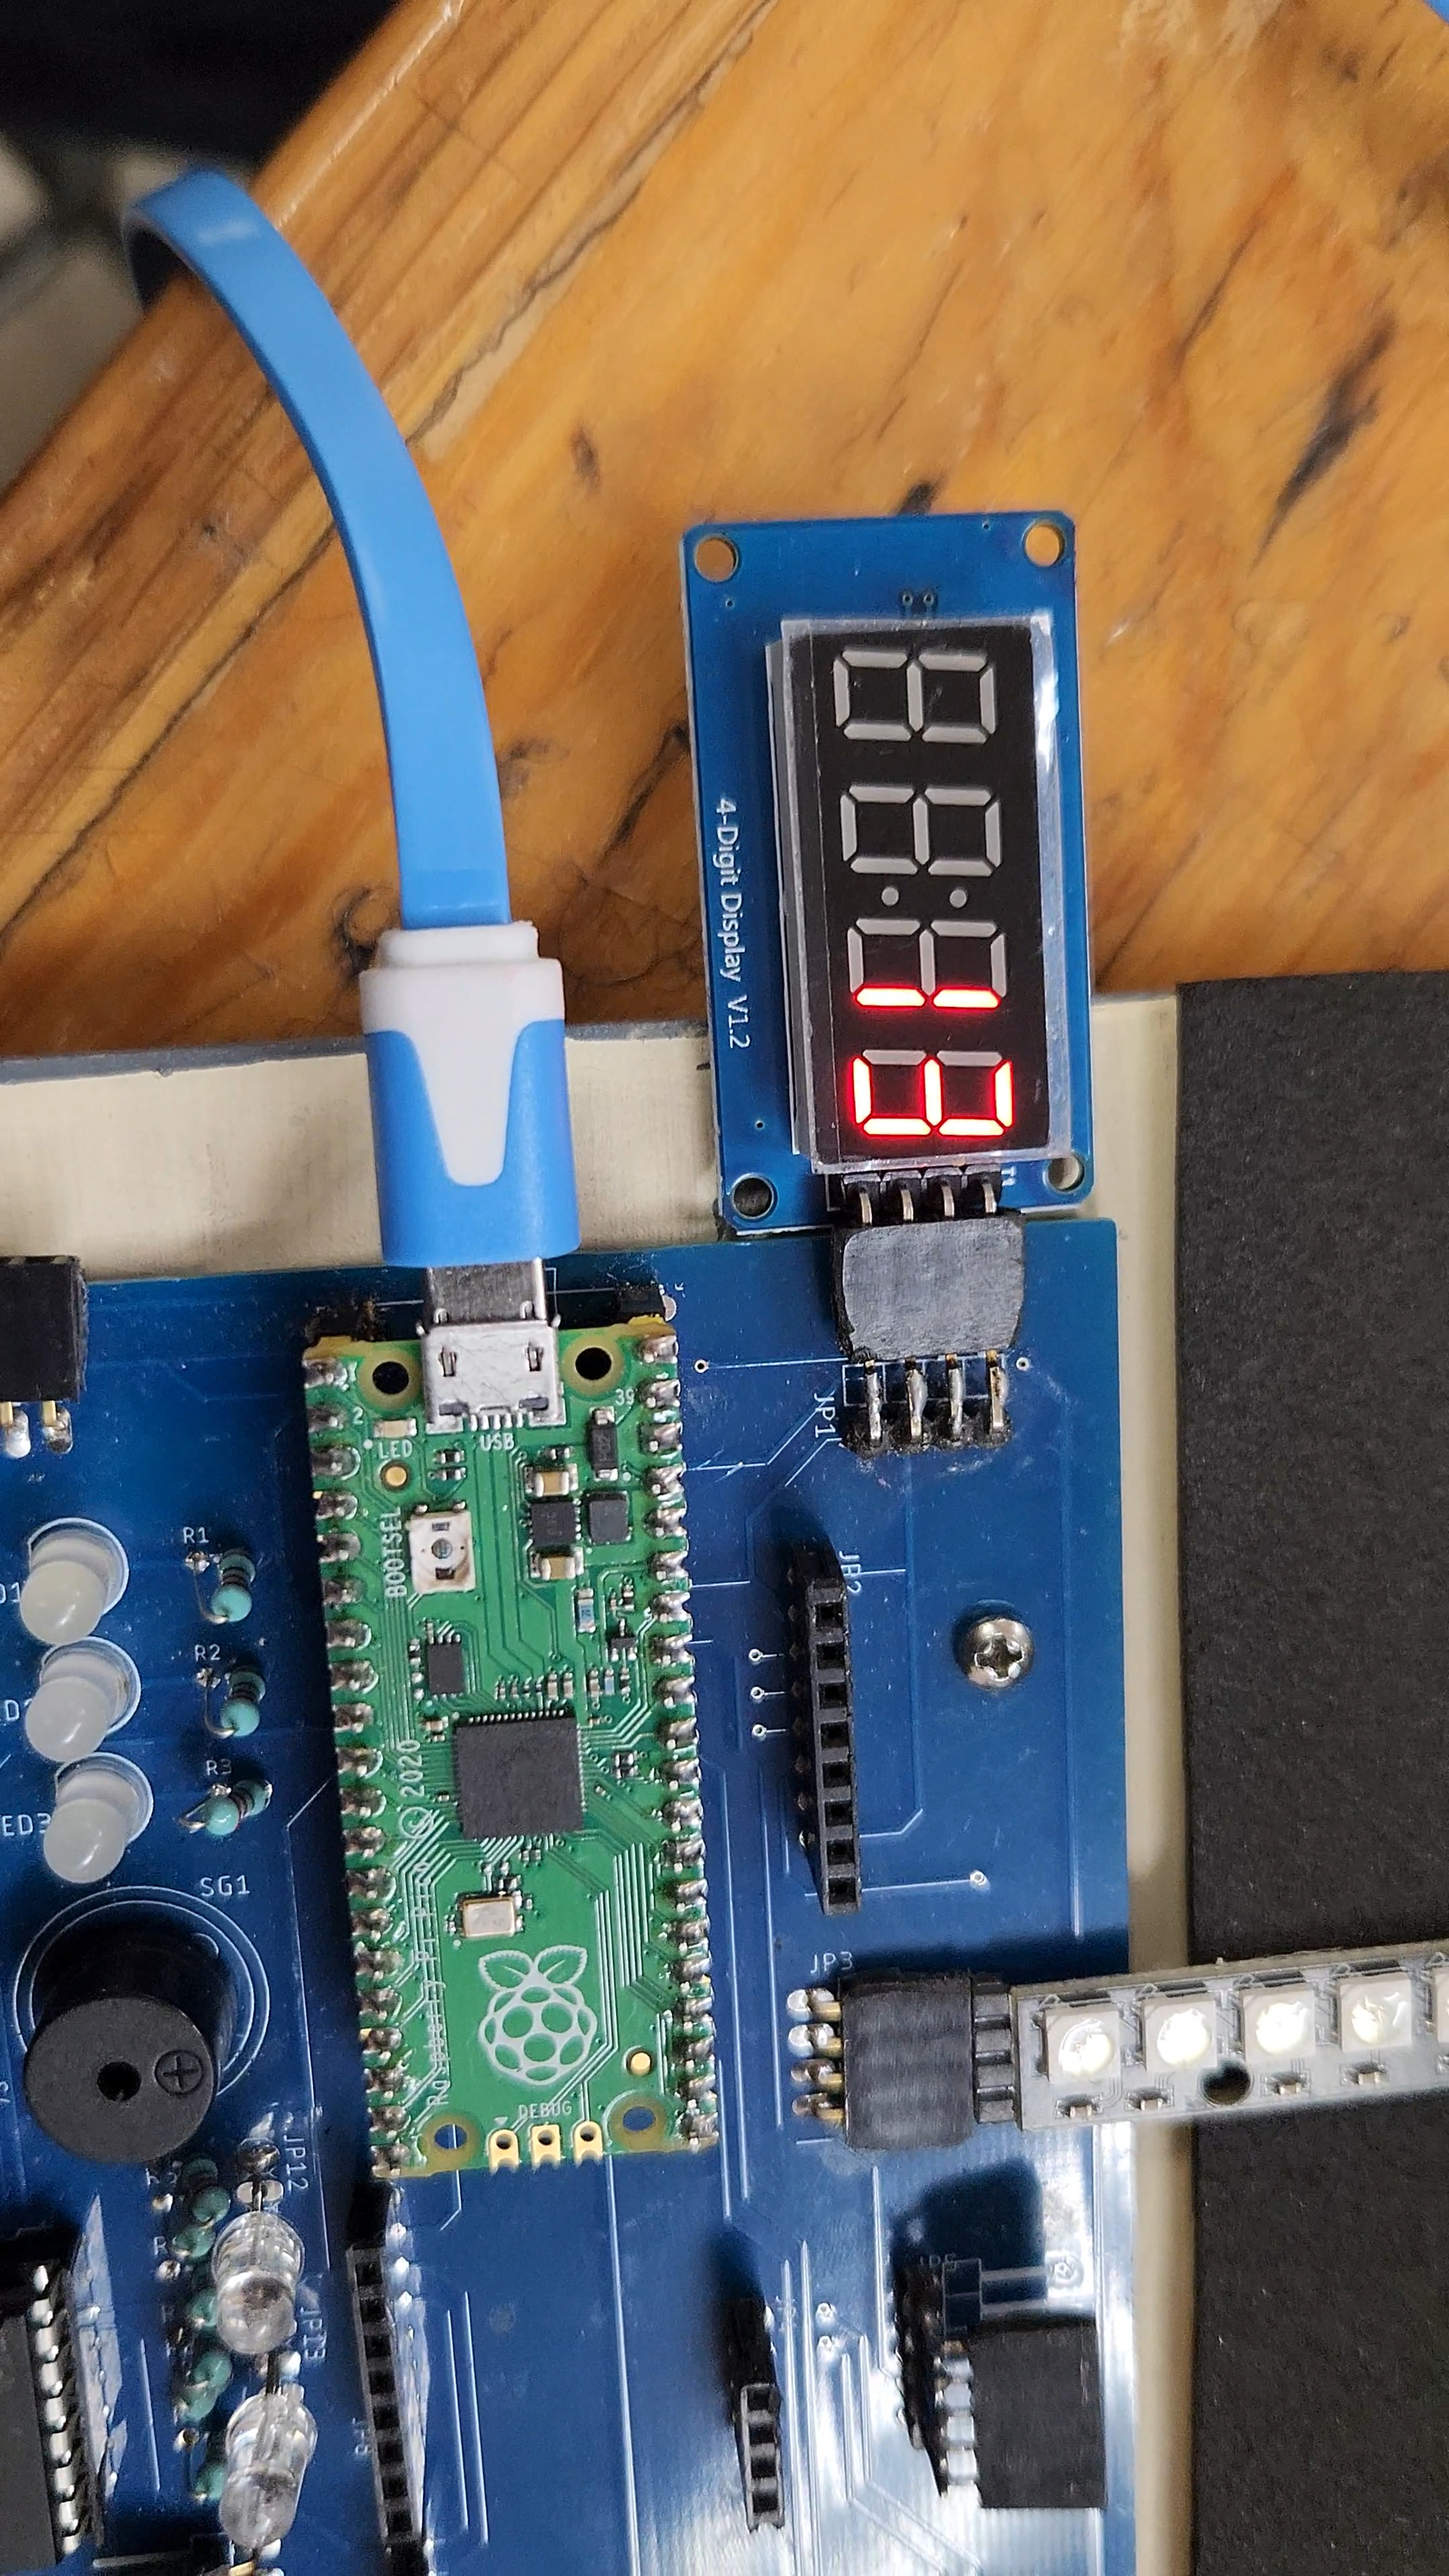
\includegraphics[width=0.6\textwidth, angle=90]{img/Actividad4/Act4_1.jpg}
        \caption{Valor 19}
    \end{minipage}
    \begin{minipage}{0.3\textwidth}
        \centering
        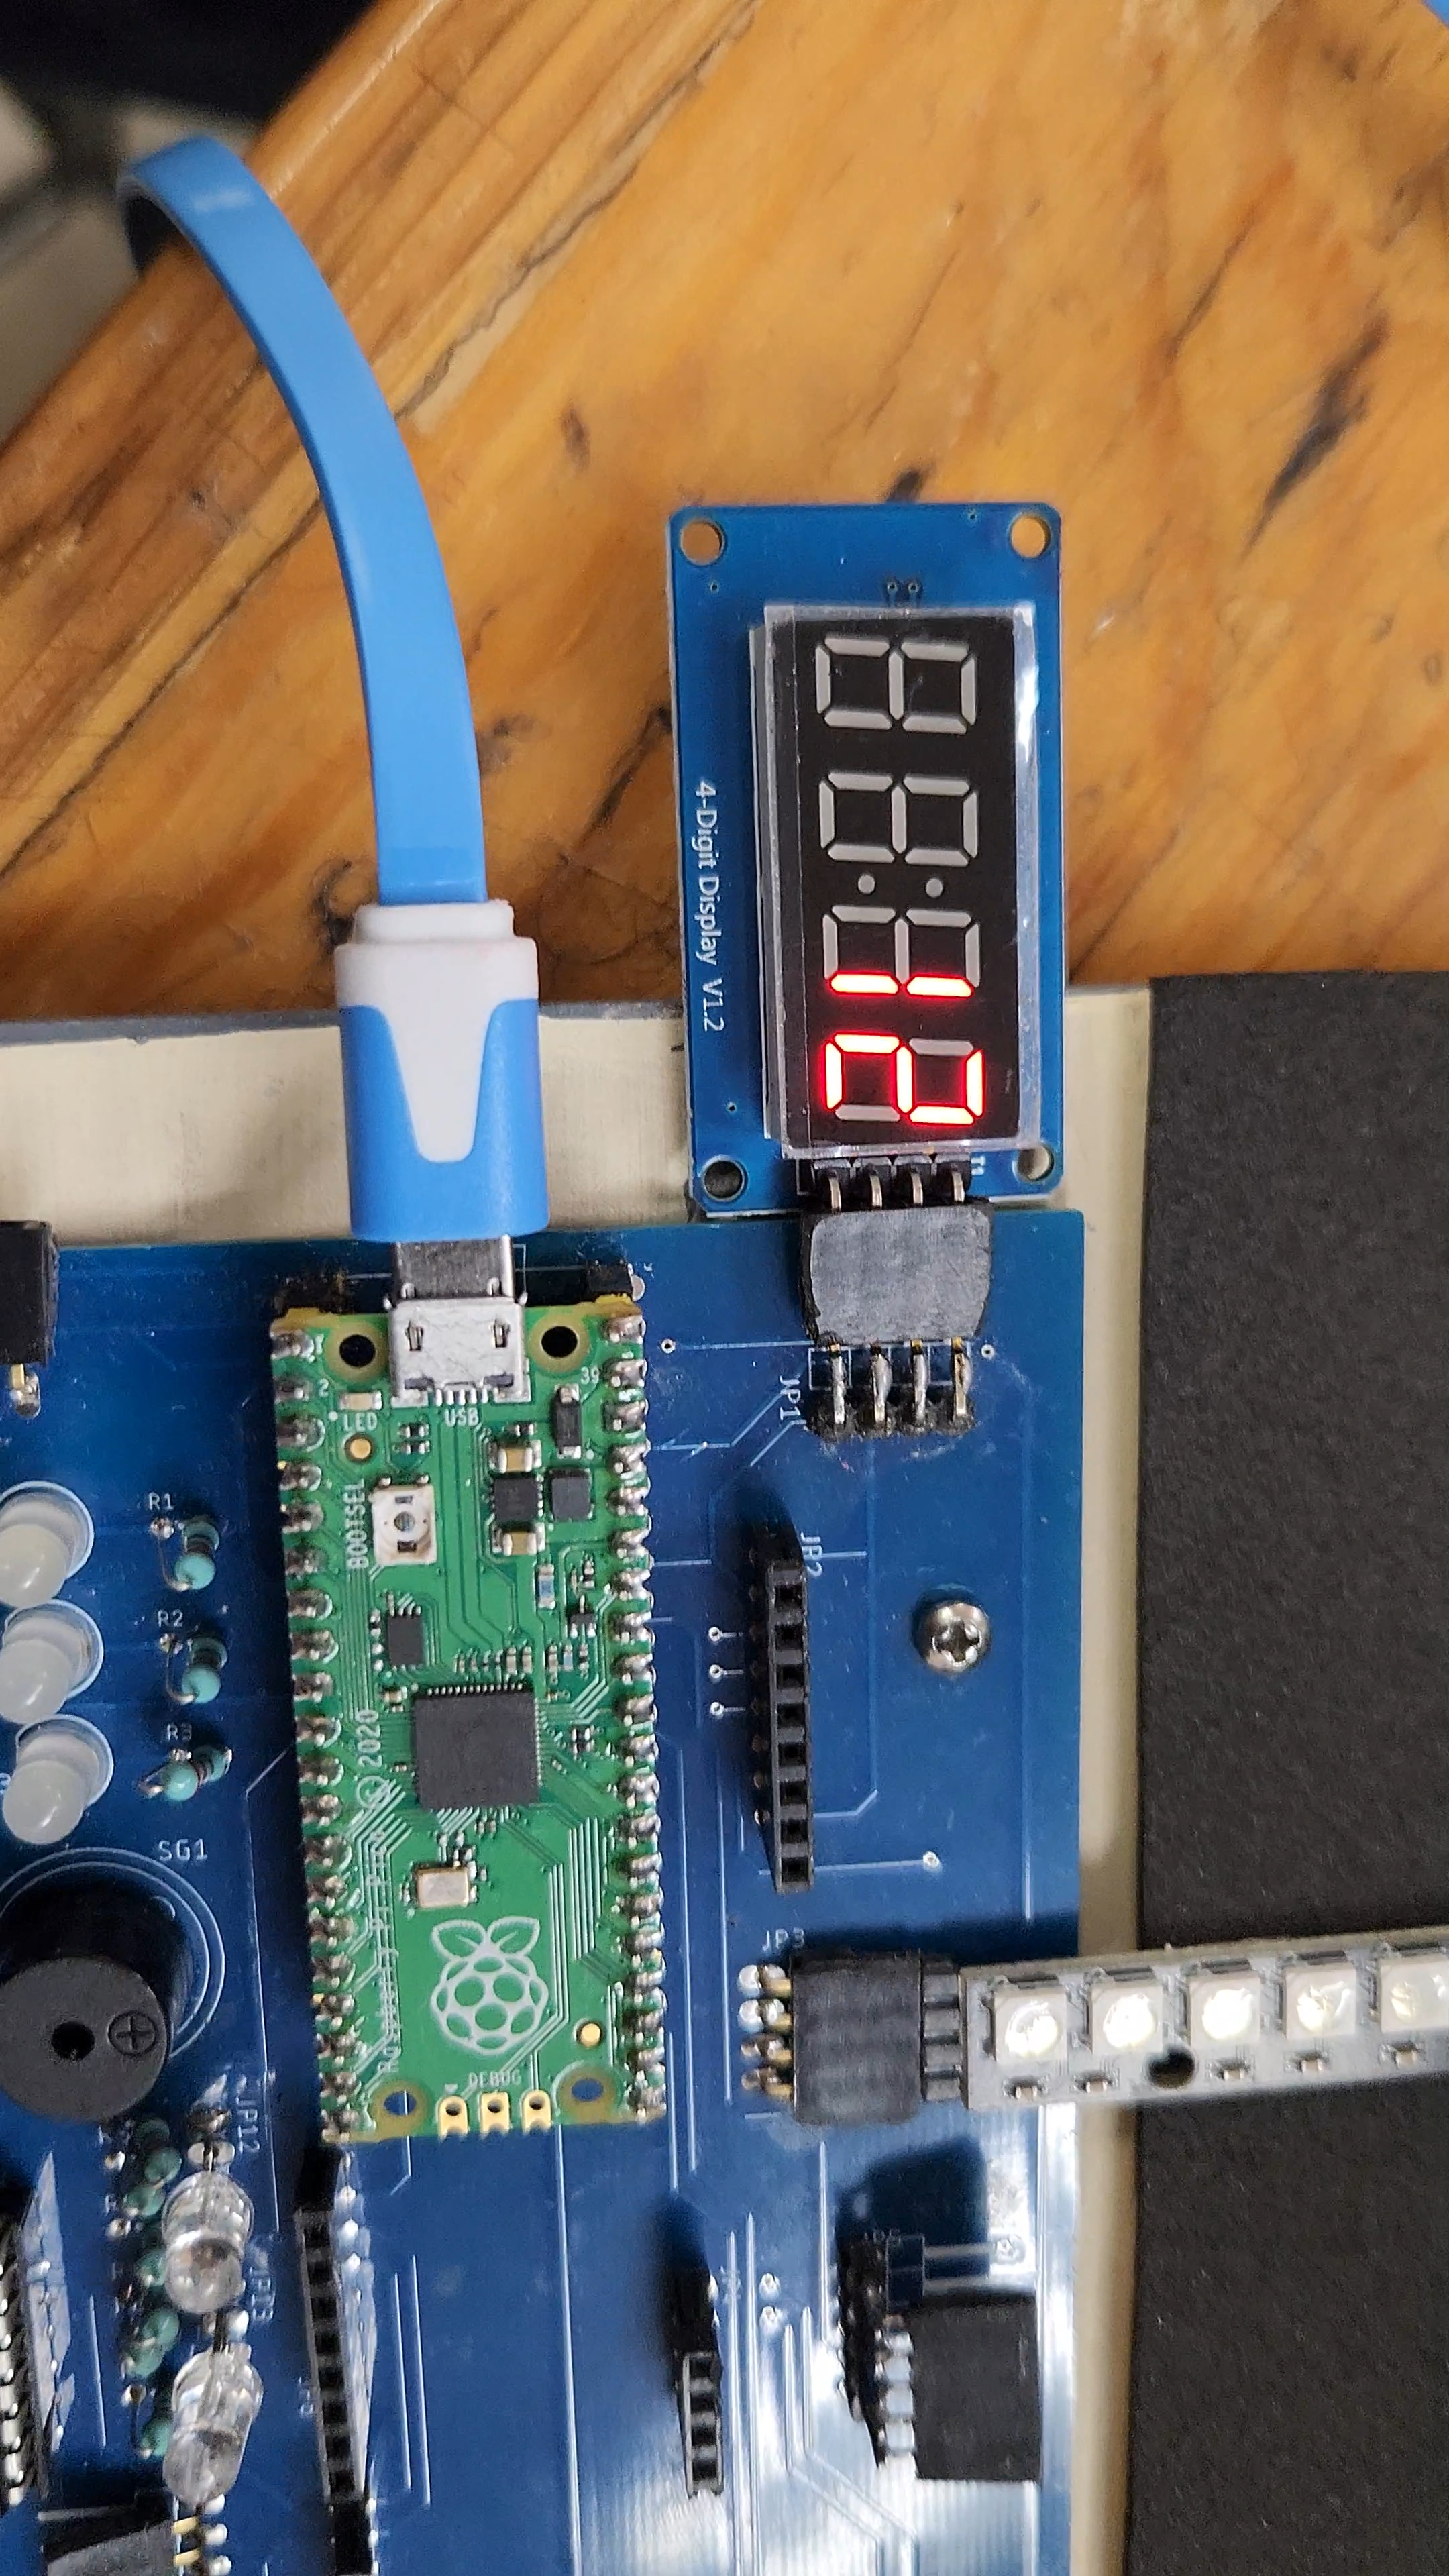
\includegraphics[width=0.6\textwidth, angle=90]{img/Actividad4/Act4_7.jpg}
        \caption{Valor 18}
    \end{minipage}
\end{figure}

\begin{figure}[H]
    \centering
    \begin{minipage}{0.3\textwidth}
        \centering
        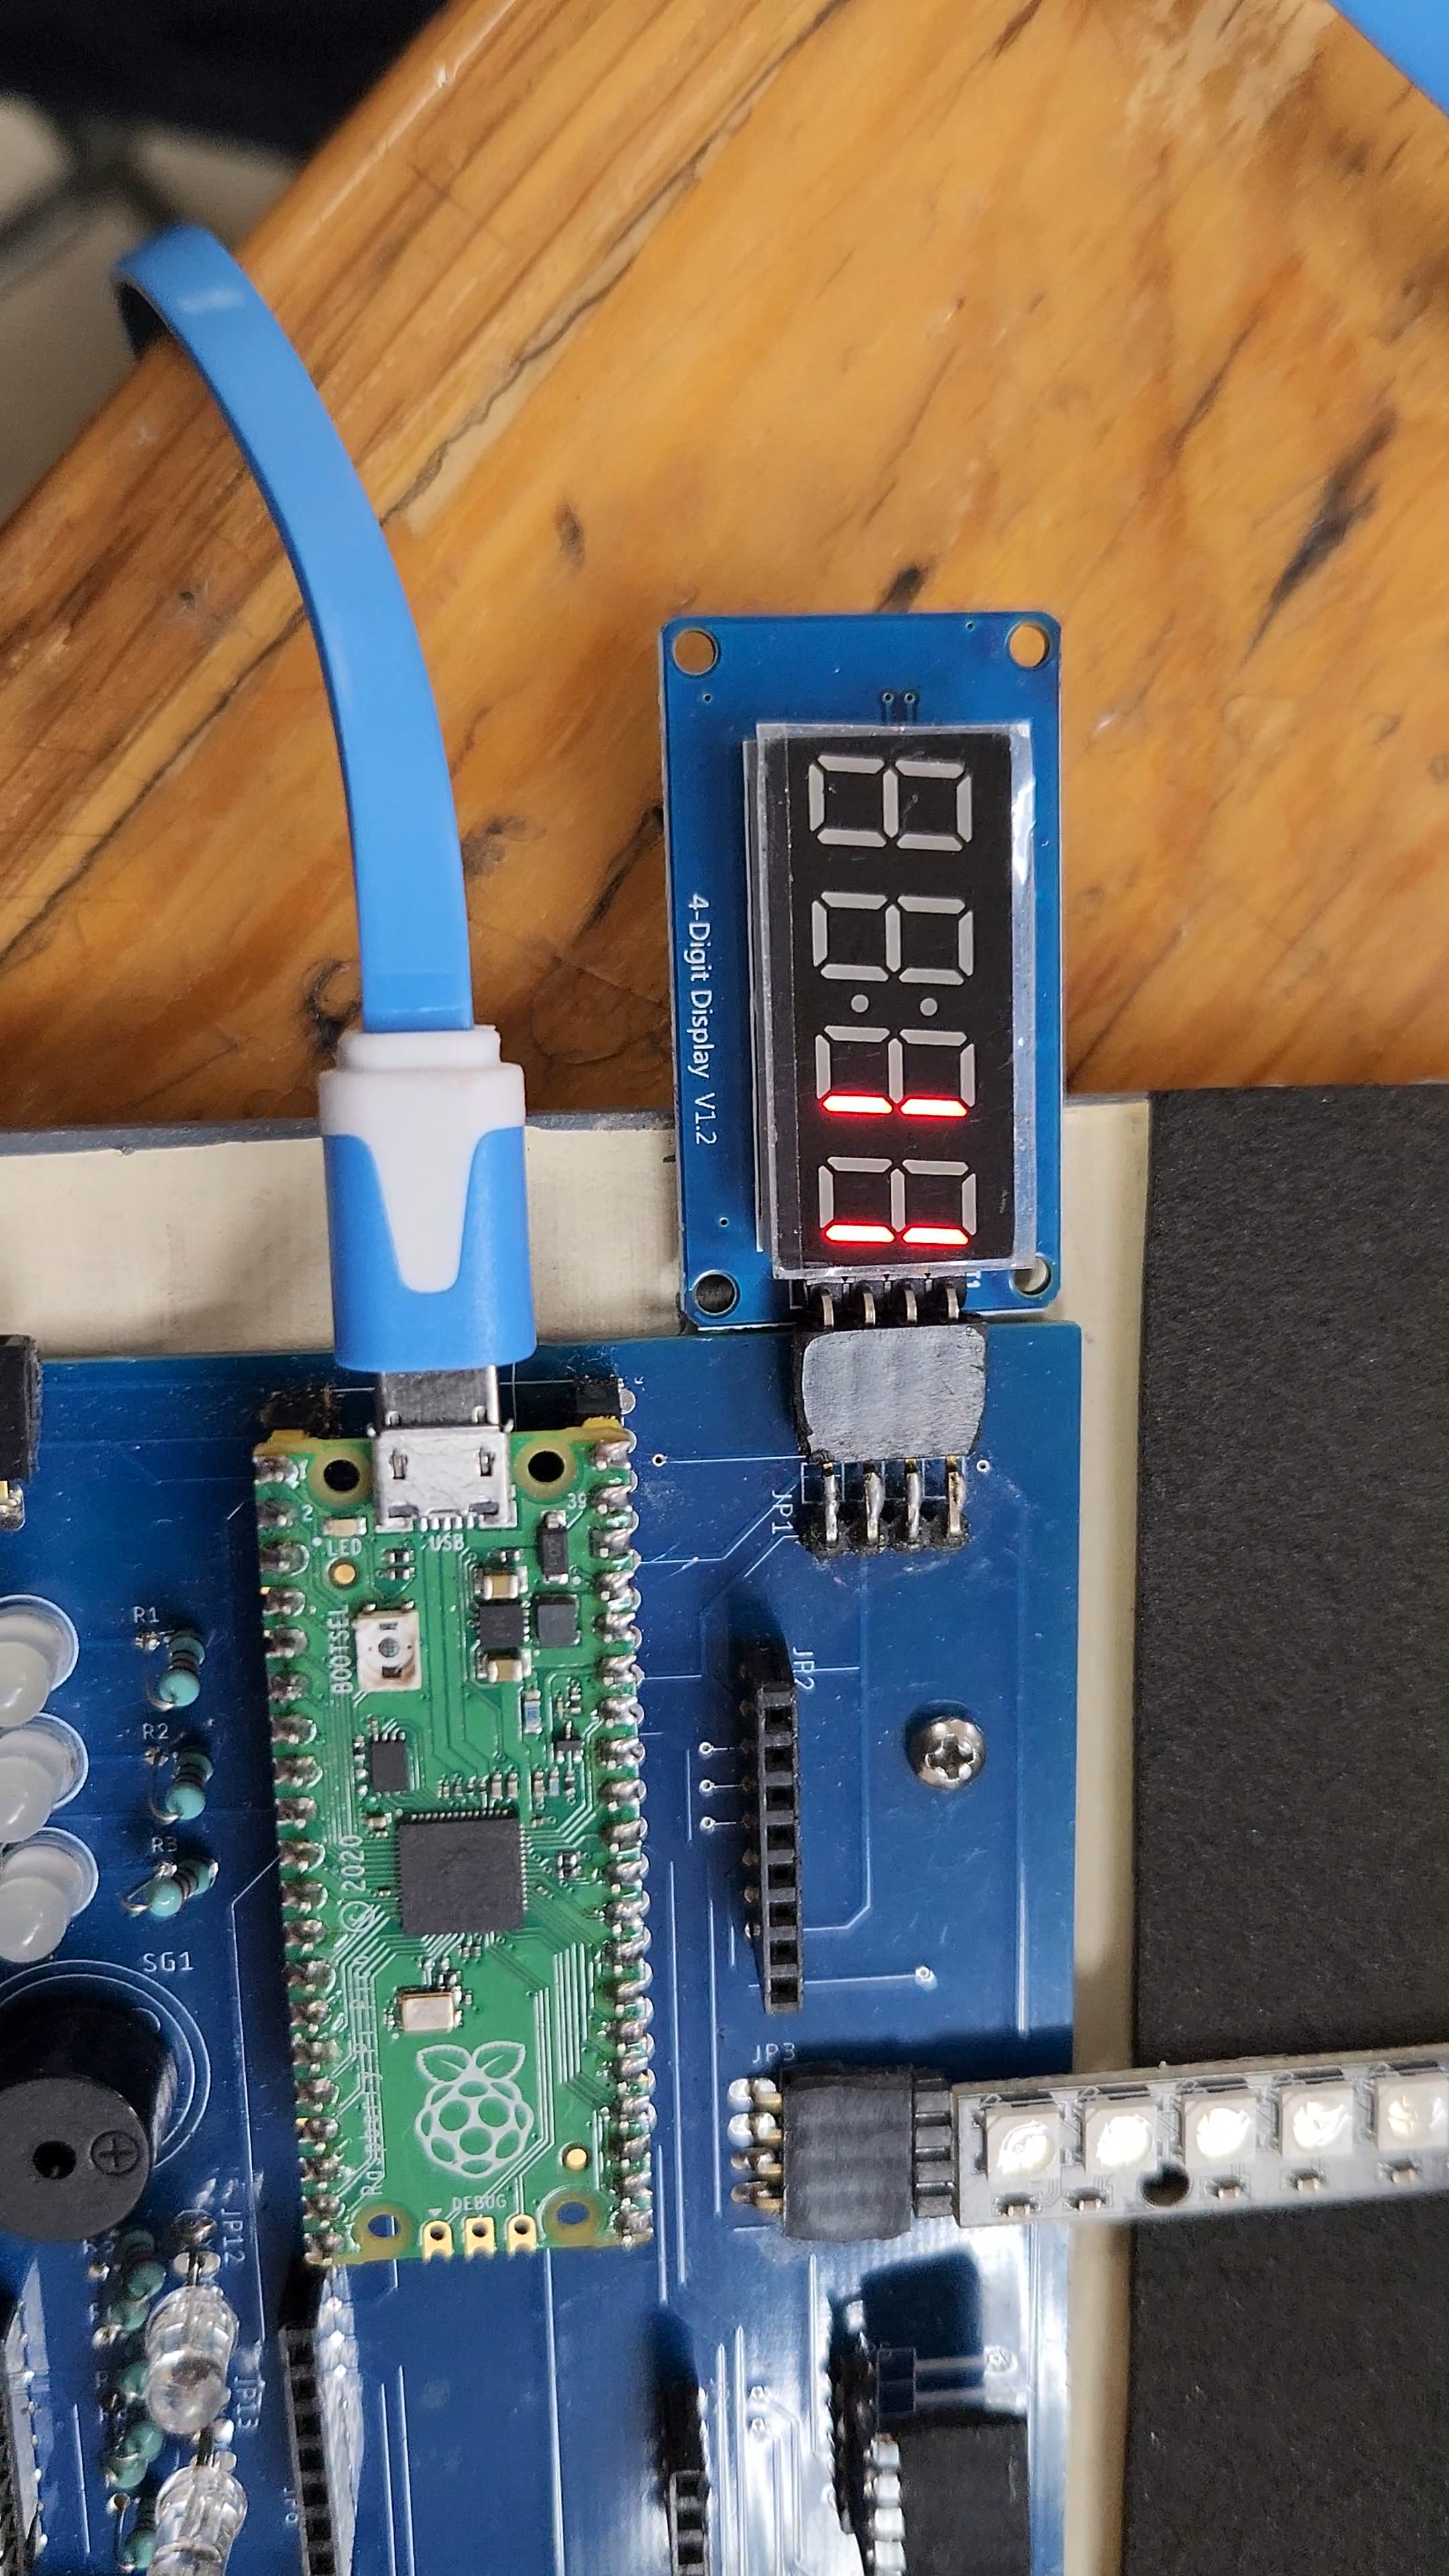
\includegraphics[width=0.6\textwidth, angle=90]{img/Actividad4/Act4_8.jpg}
        \caption{Valor 17}
    \end{minipage}
    \begin{minipage}{0.3\textwidth}
        \centering
        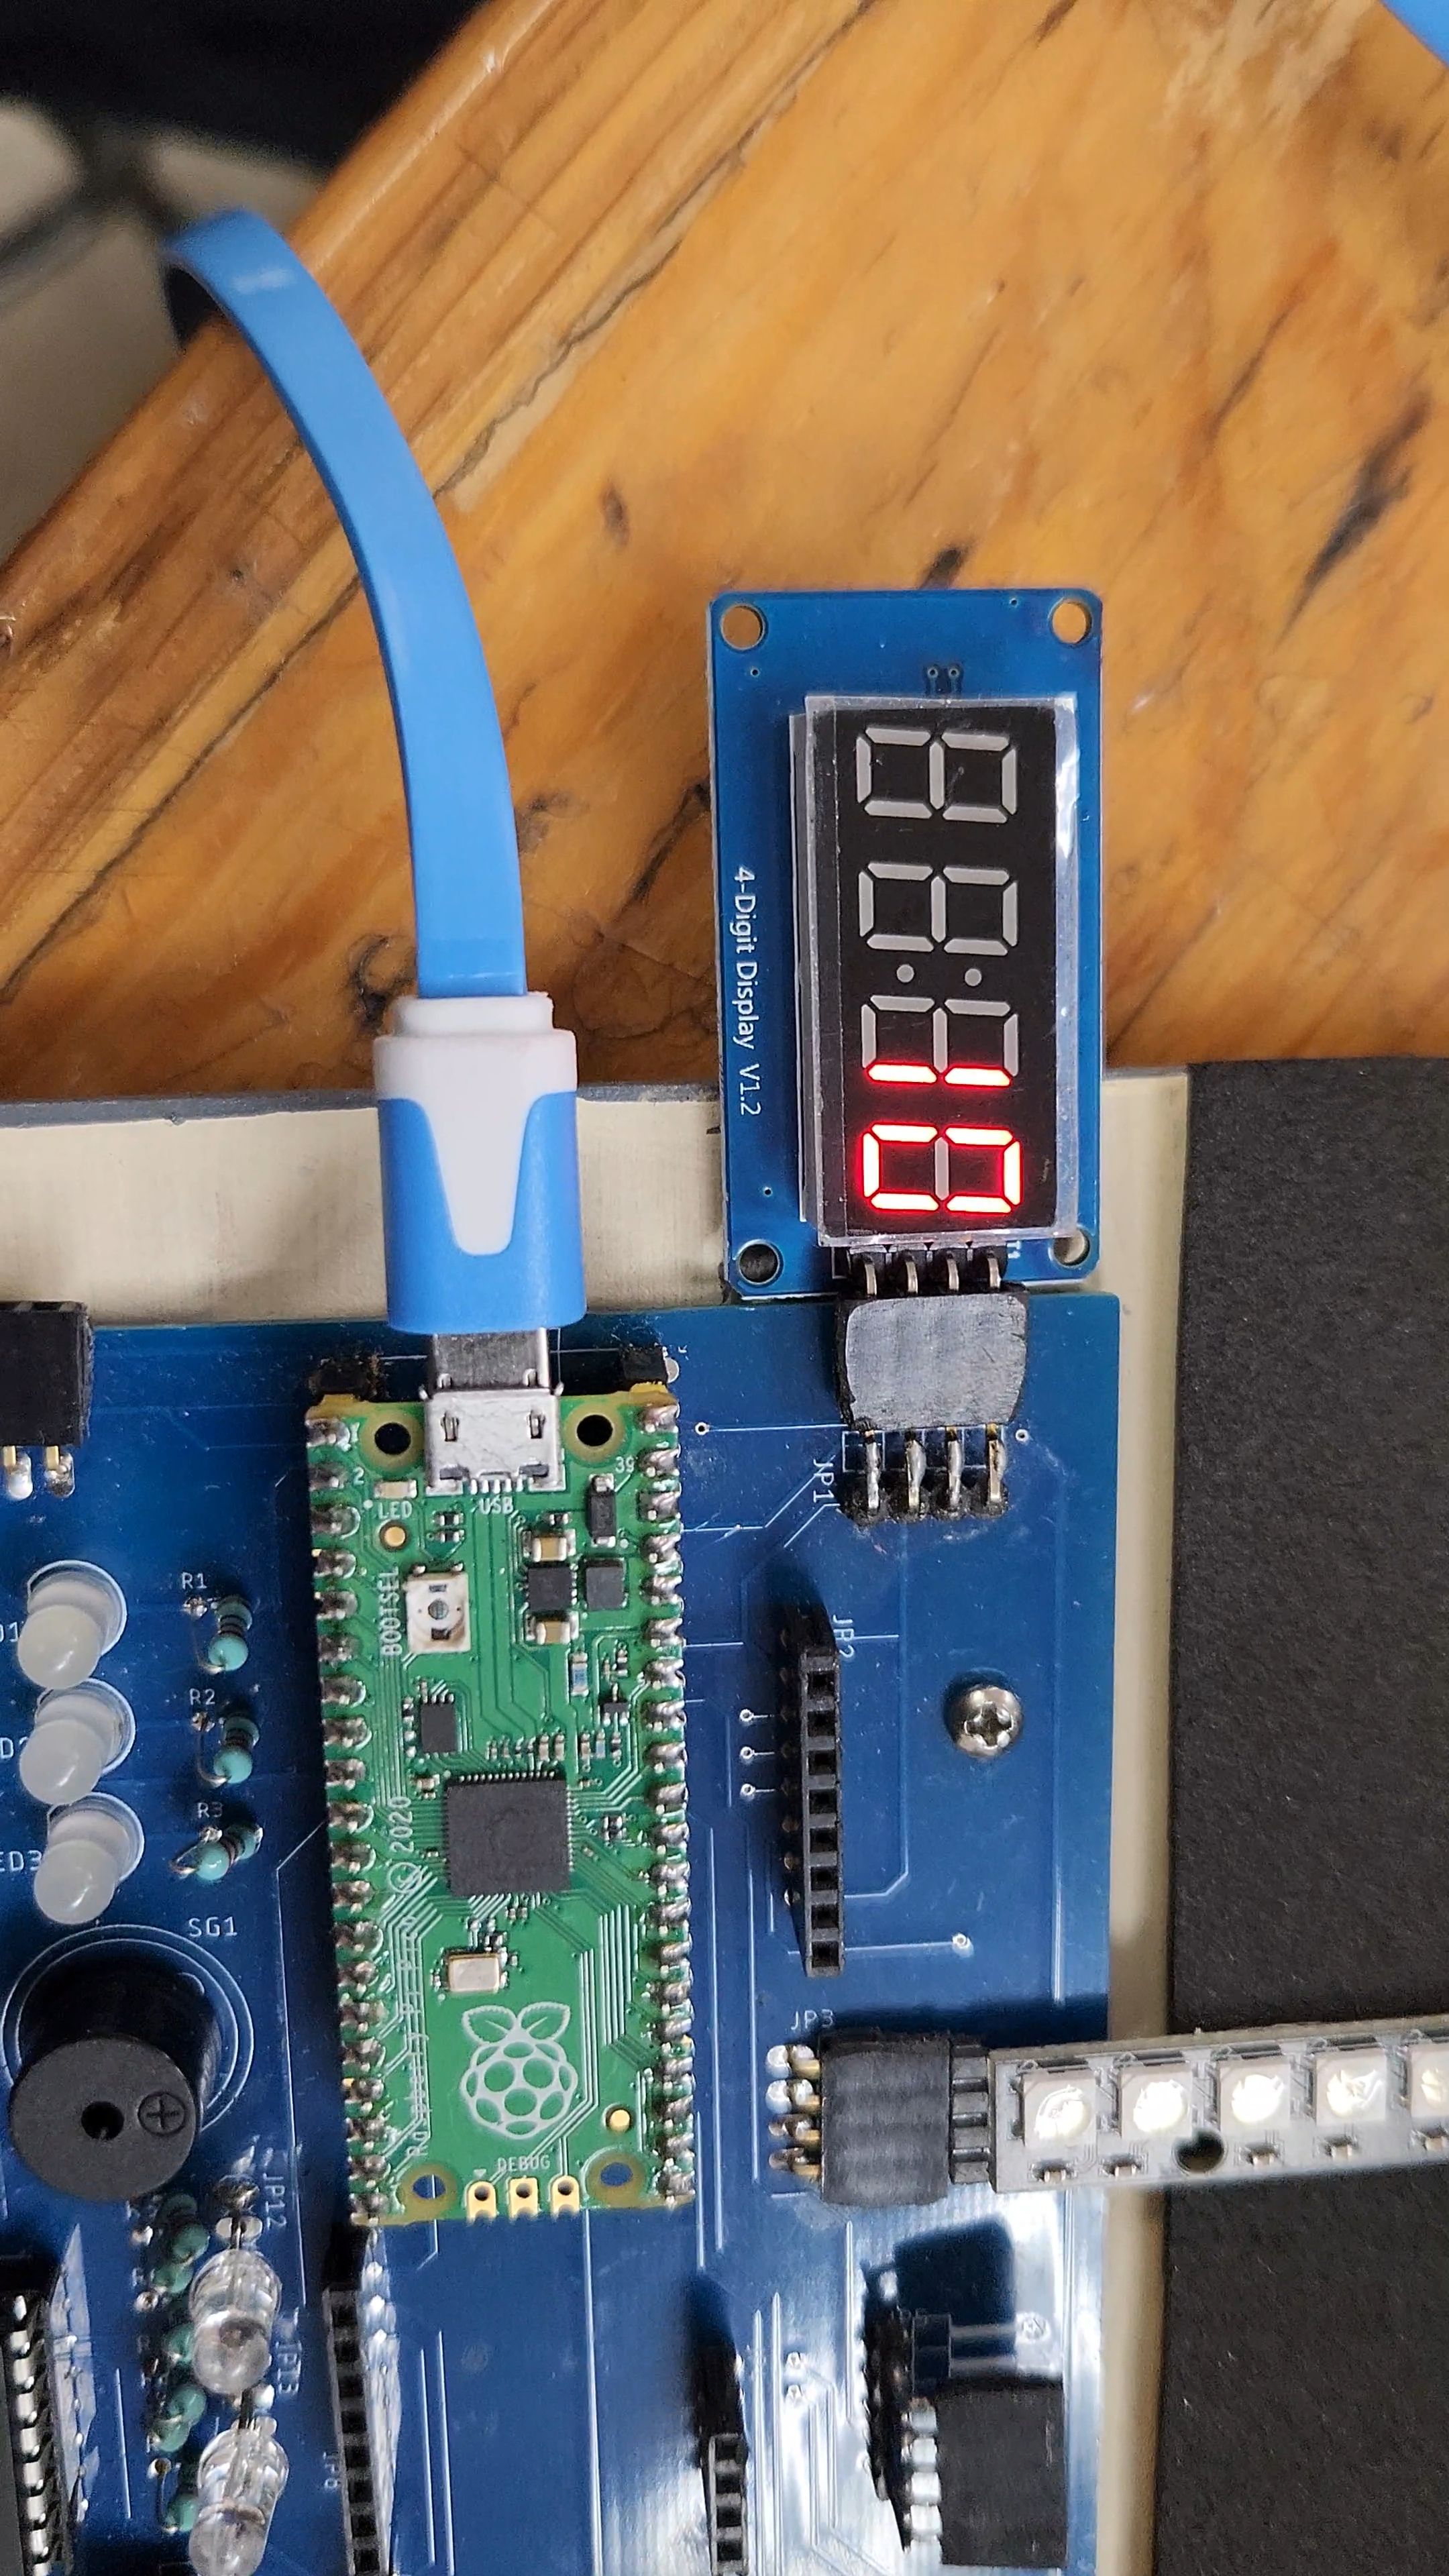
\includegraphics[width=0.6\textwidth, angle=90]{img/Actividad4/Act4_9.jpg}
        \caption{Valor 16}
    \end{minipage}
    \begin{minipage}{0.3\textwidth}
        \centering
        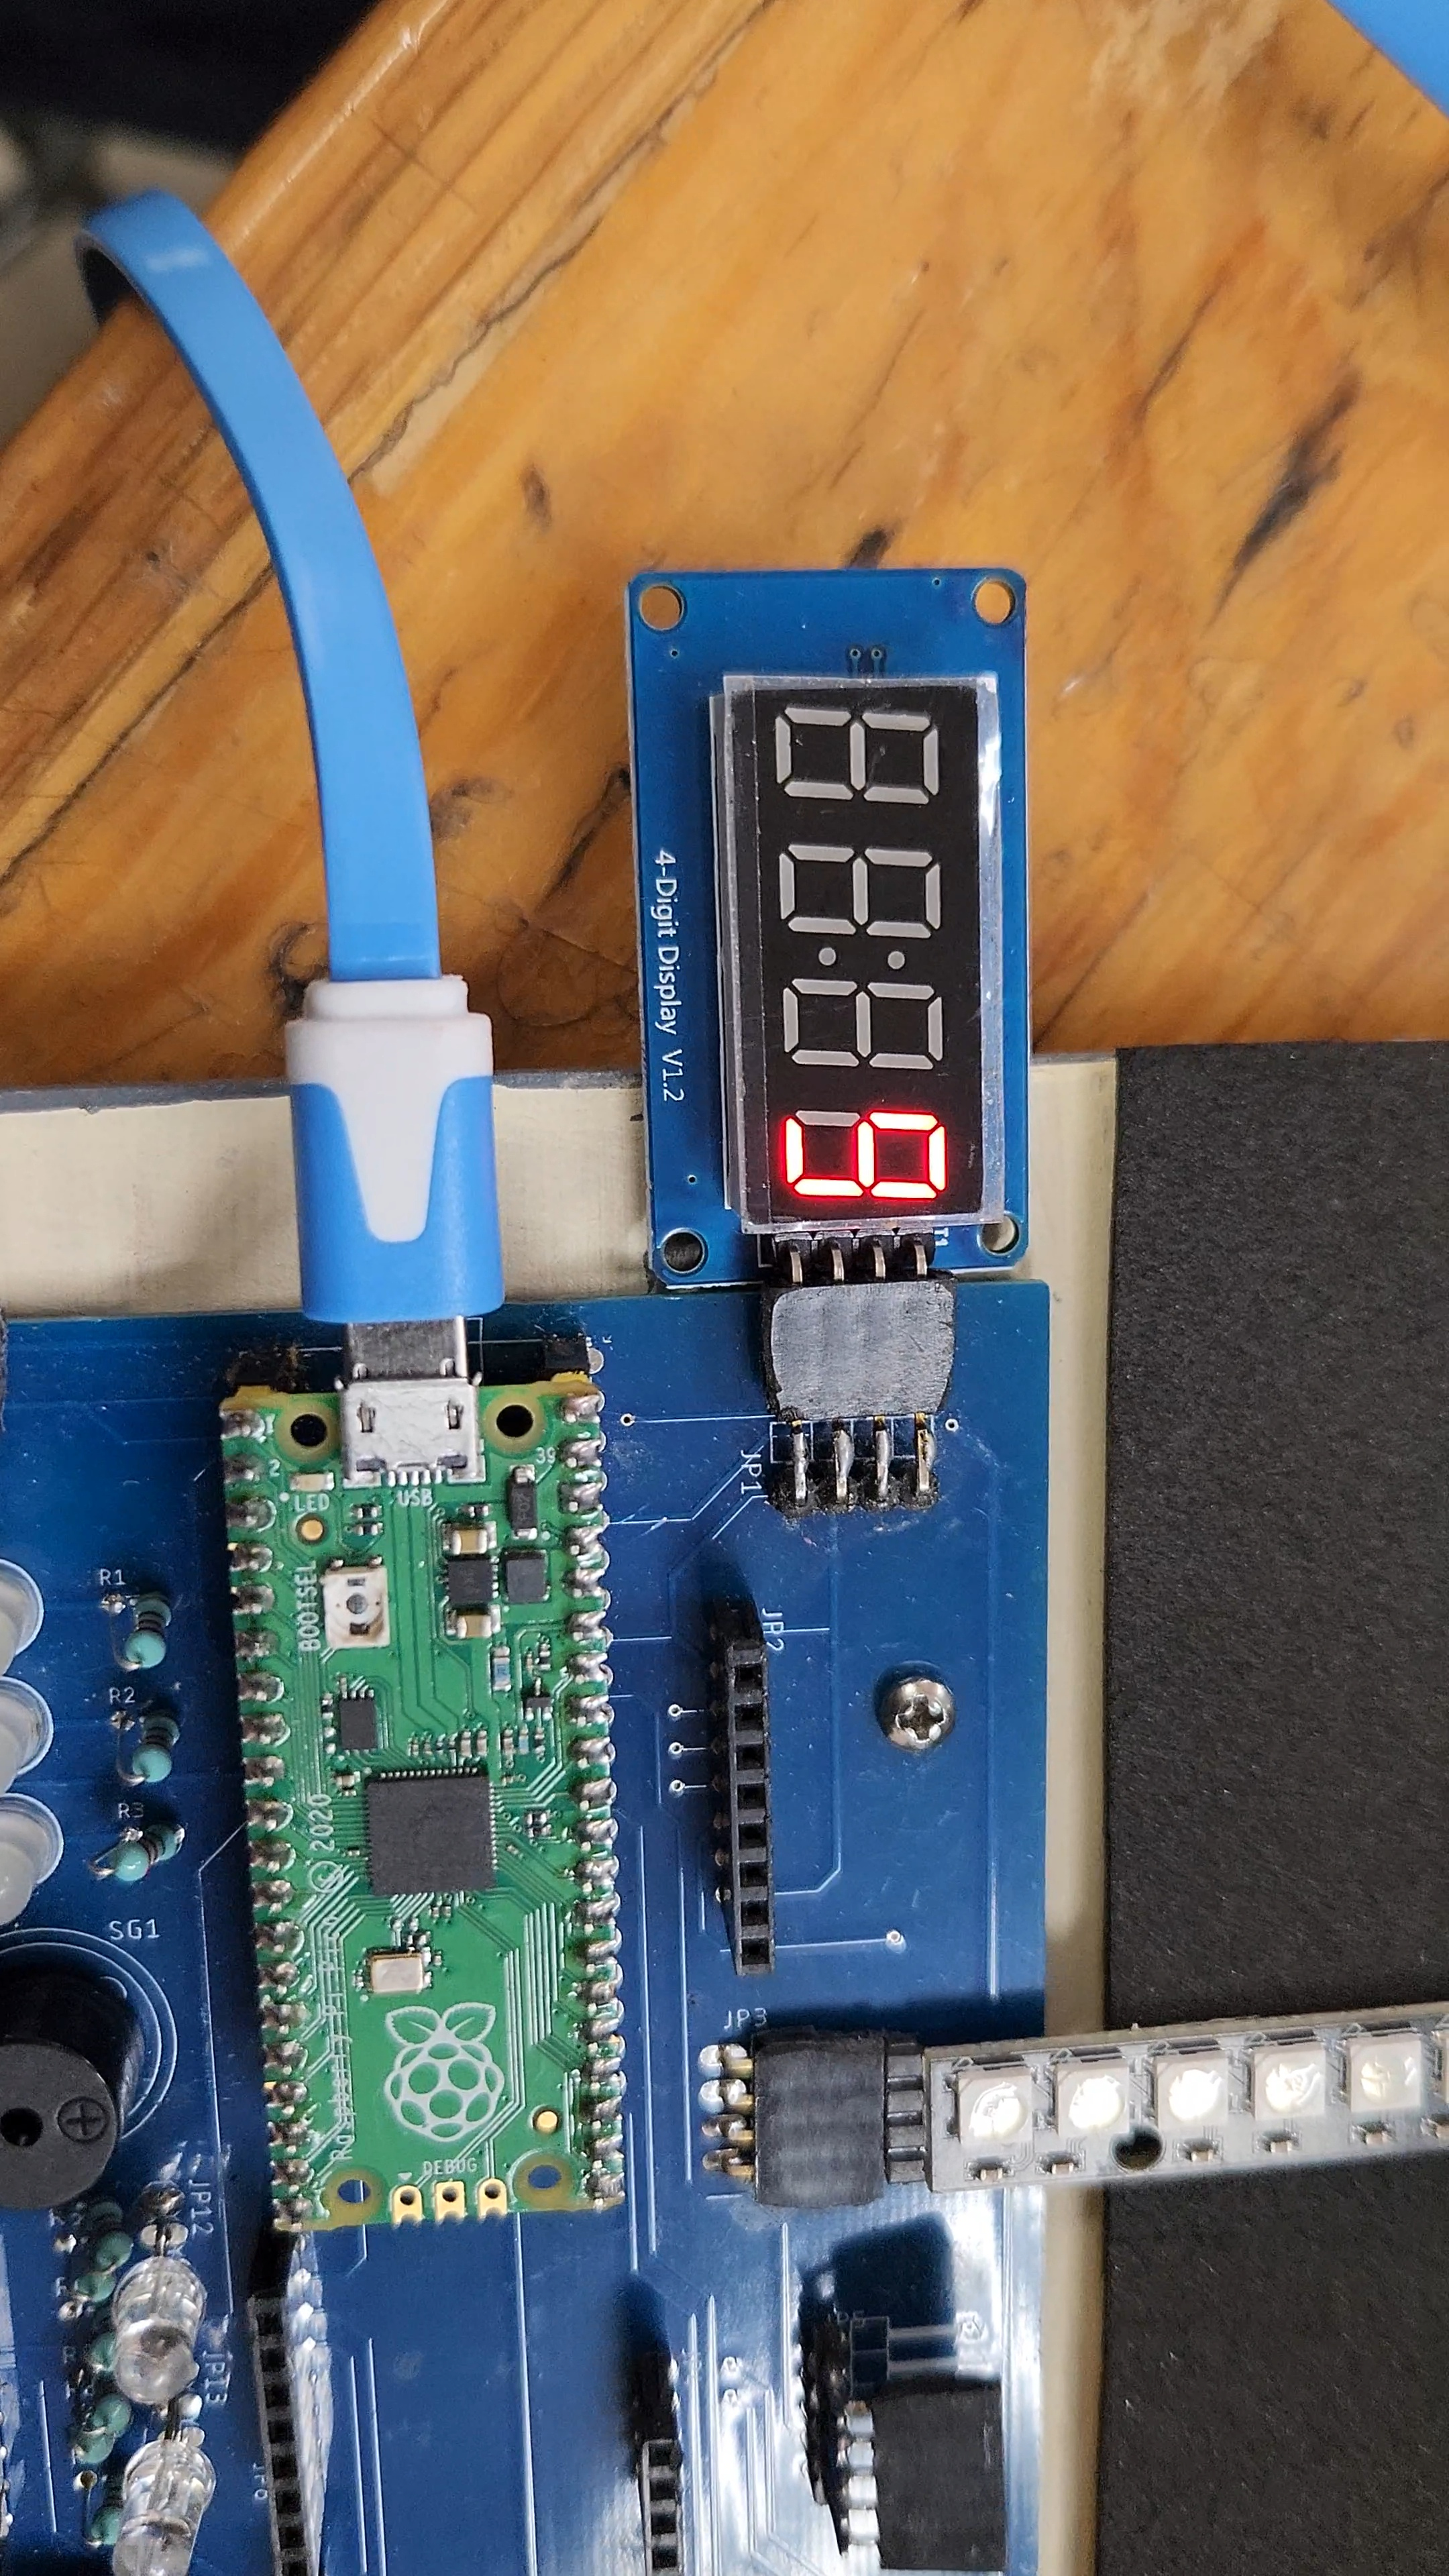
\includegraphics[width=0.6\textwidth, angle=90]{img/Actividad4/Act4_10.jpg}
        \caption{Valor 15}
    \end{minipage}
\end{figure}

\begin{figure}[H]
    \centering
    \begin{minipage}{0.3\textwidth}
        \centering
        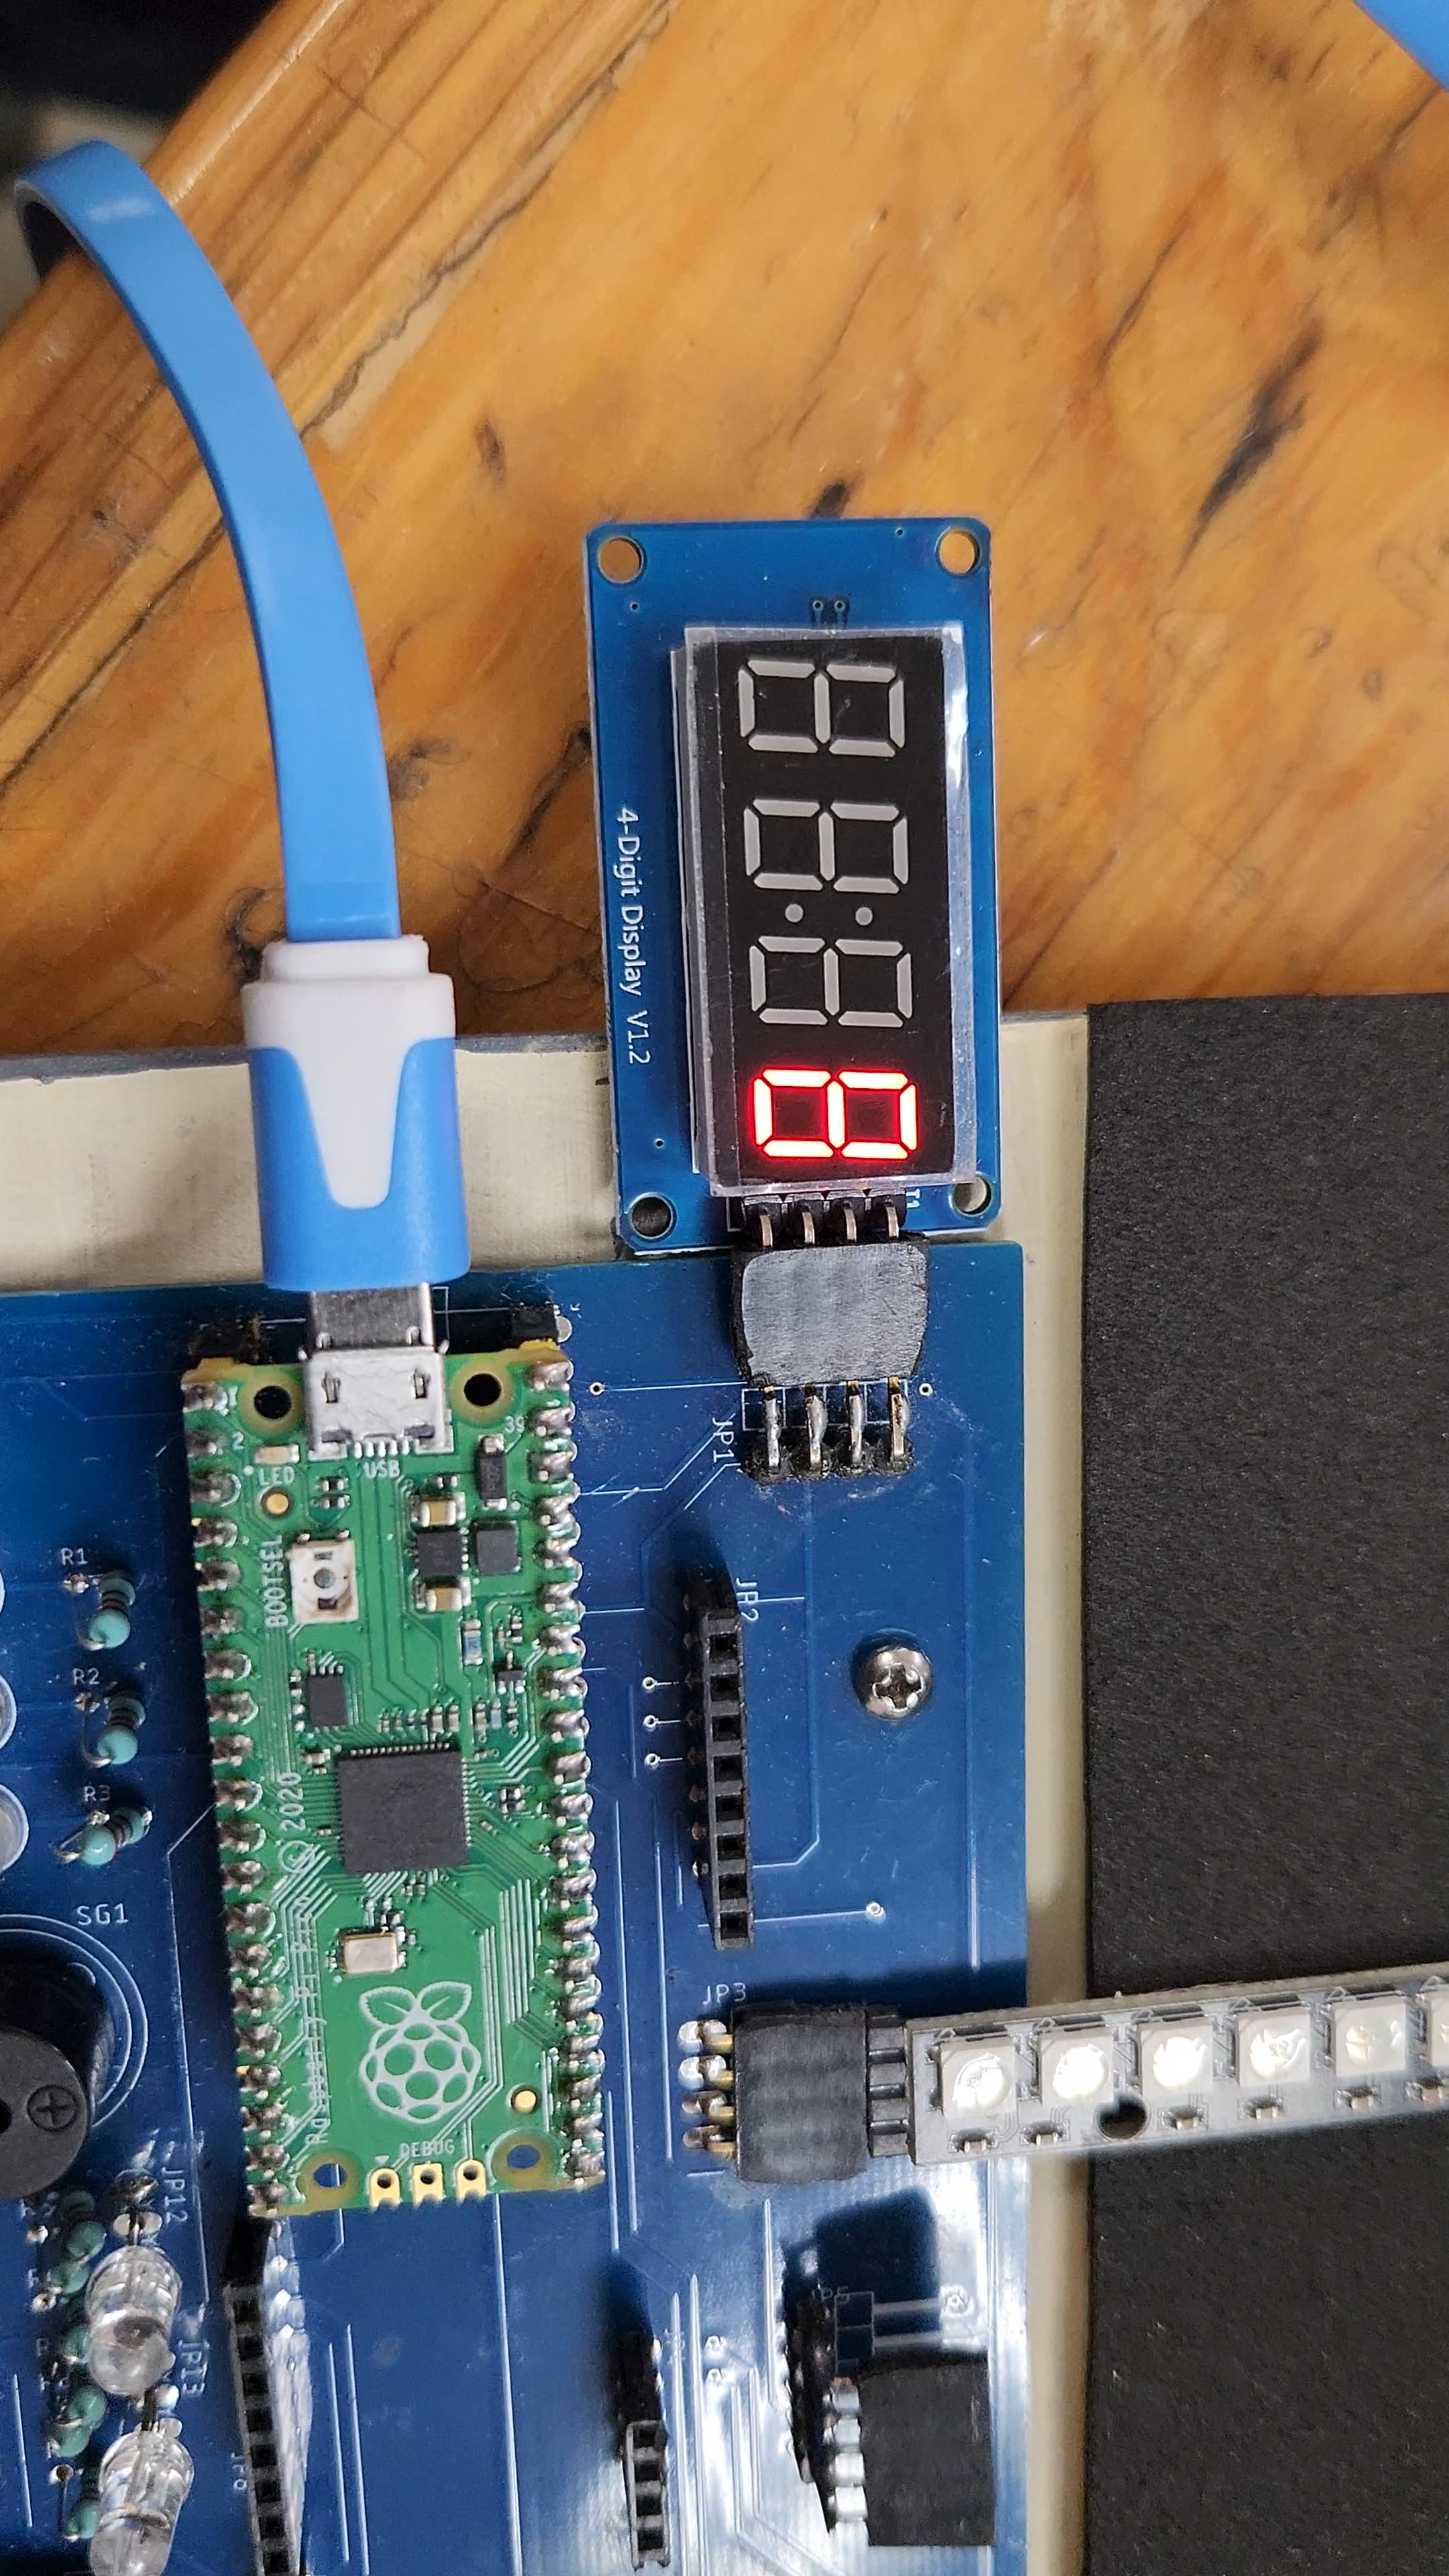
\includegraphics[width=0.6\textwidth, angle=90]{img/Actividad4/Act4_11.jpg}
        \caption{Valor 14}
    \end{minipage}
    \begin{minipage}{0.3\textwidth}
        \centering
        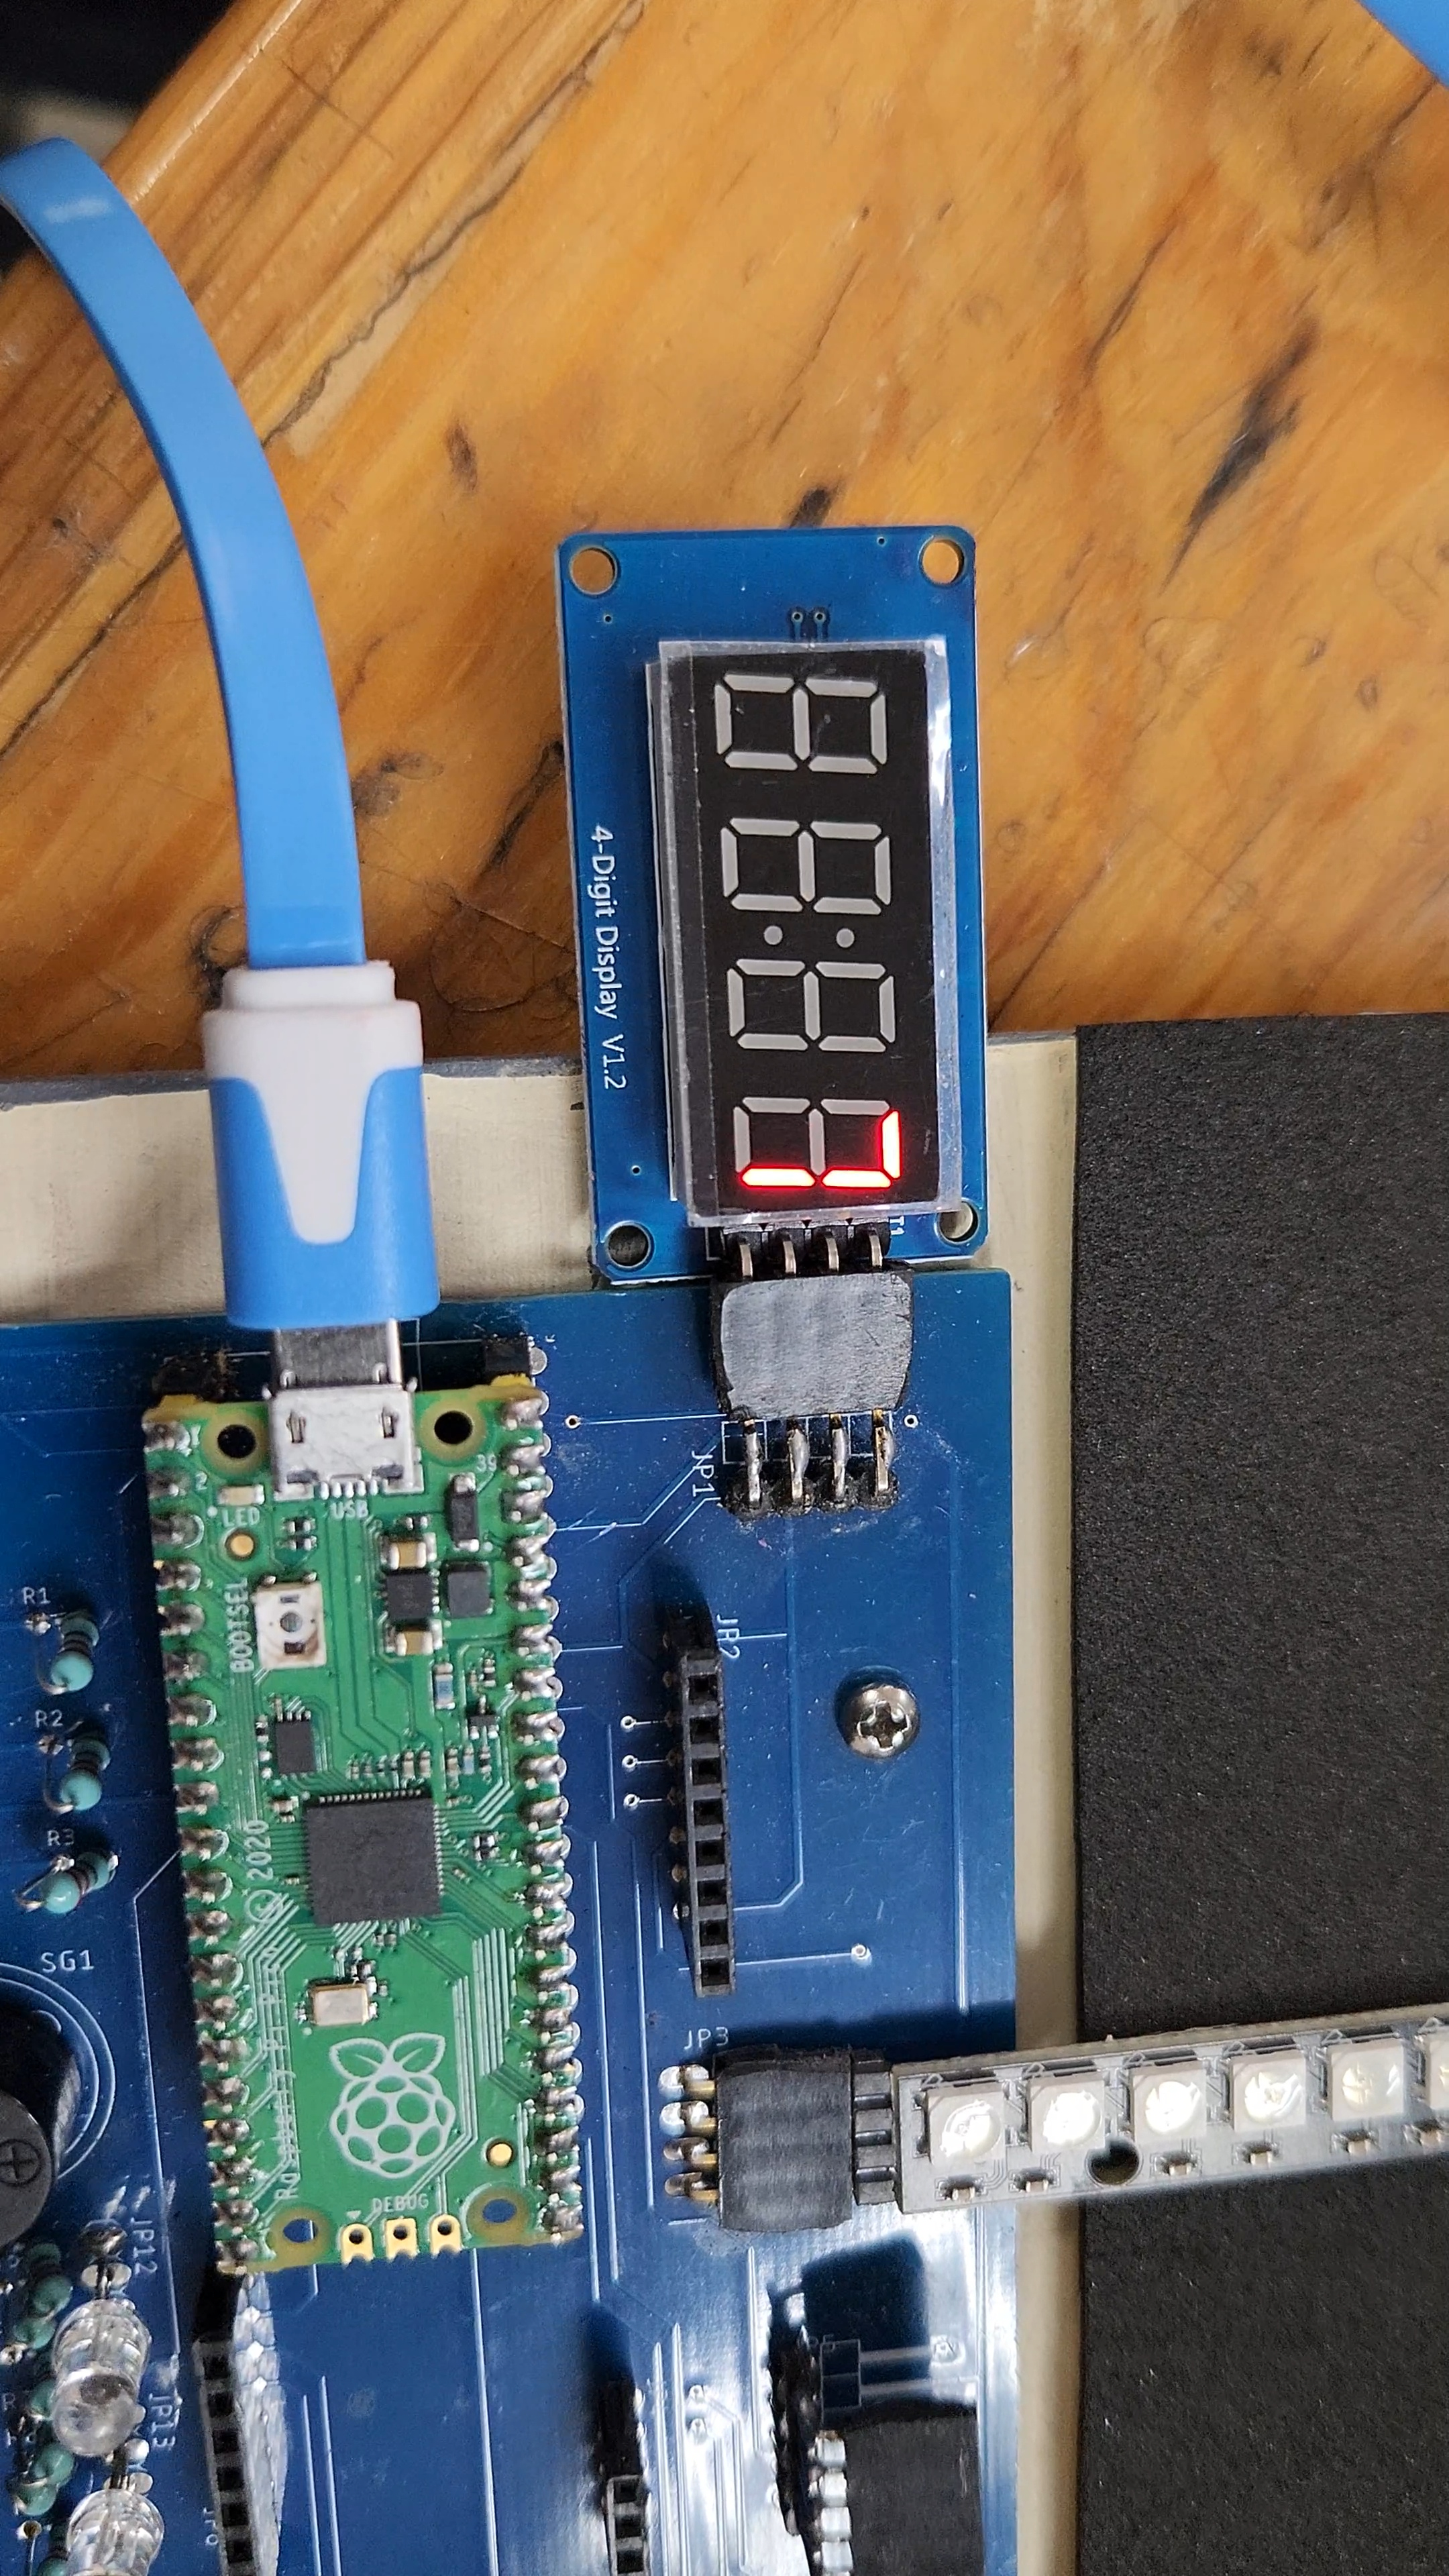
\includegraphics[width=0.6\textwidth, angle=90]{img/Actividad4/Act4_12.jpg}
        \caption{Valor 13}
    \end{minipage}
    \begin{minipage}{0.3\textwidth}
        \centering
        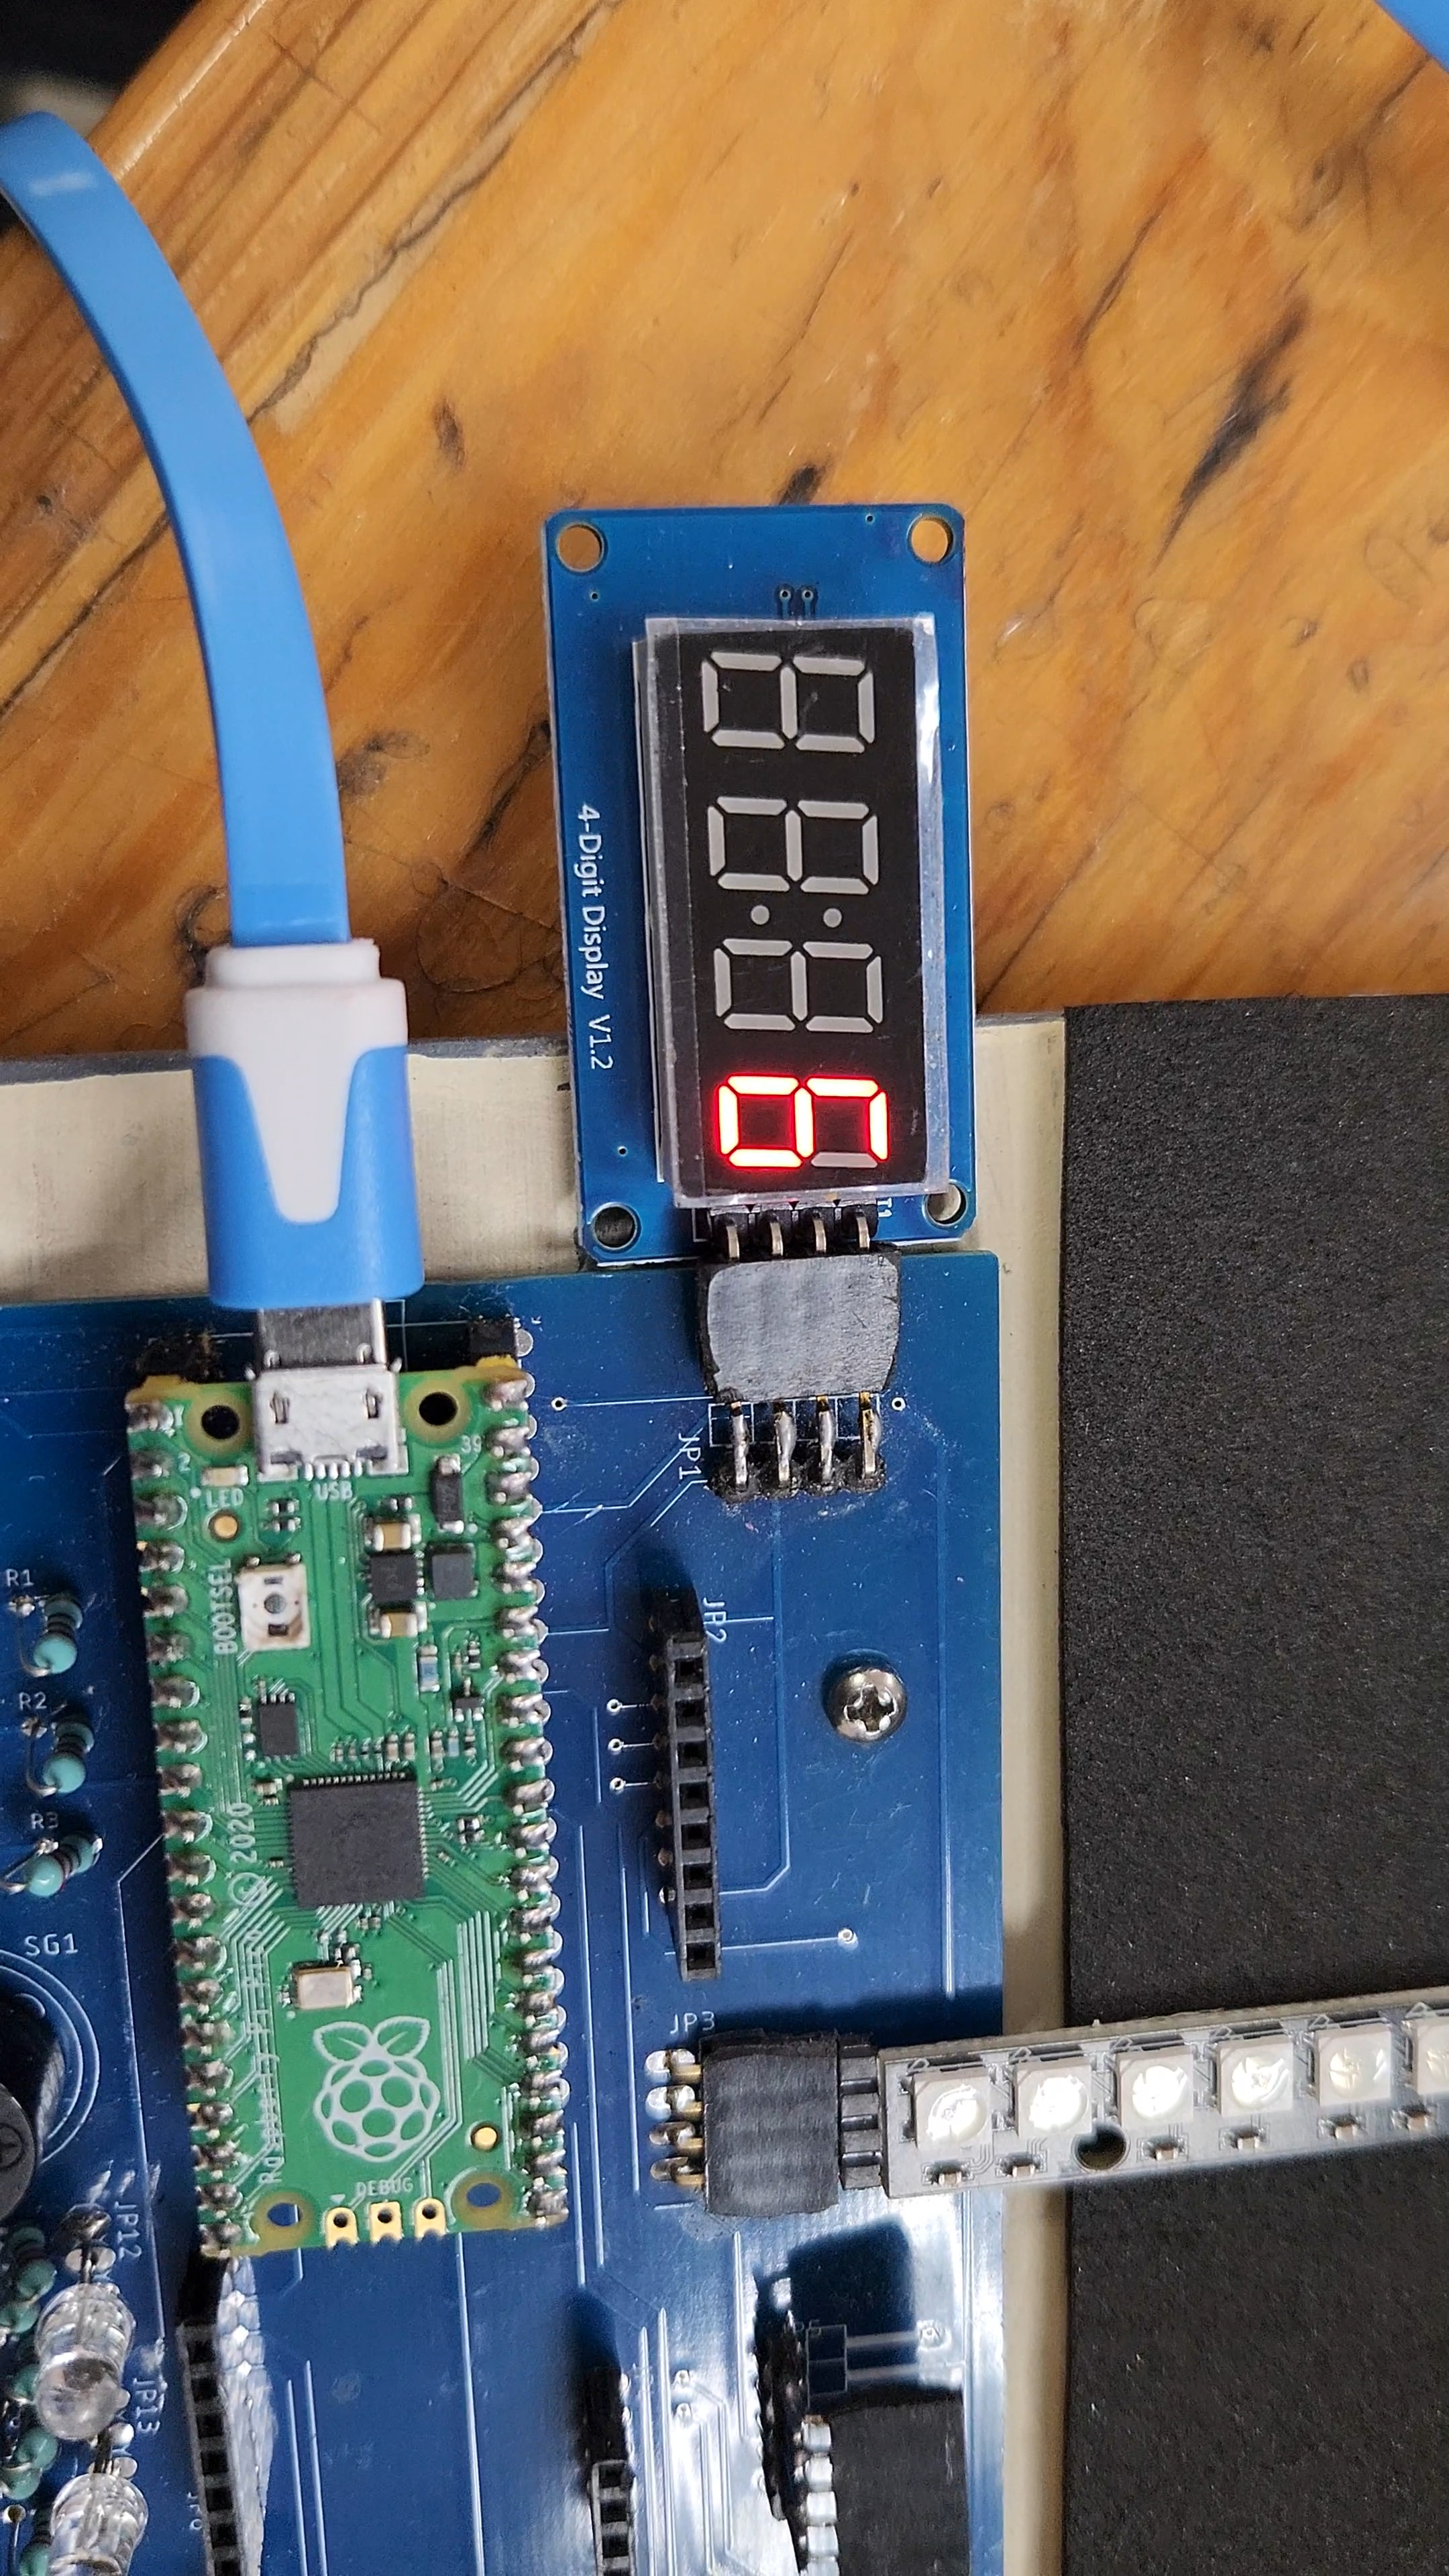
\includegraphics[width=0.6\textwidth, angle=90]{img/Actividad4/Act4_13.jpg}
        \caption{Valor 12}
    \end{minipage}
\end{figure}

\begin{figure}[H]
    \centering
    \begin{minipage}{0.3\textwidth}
        \centering
        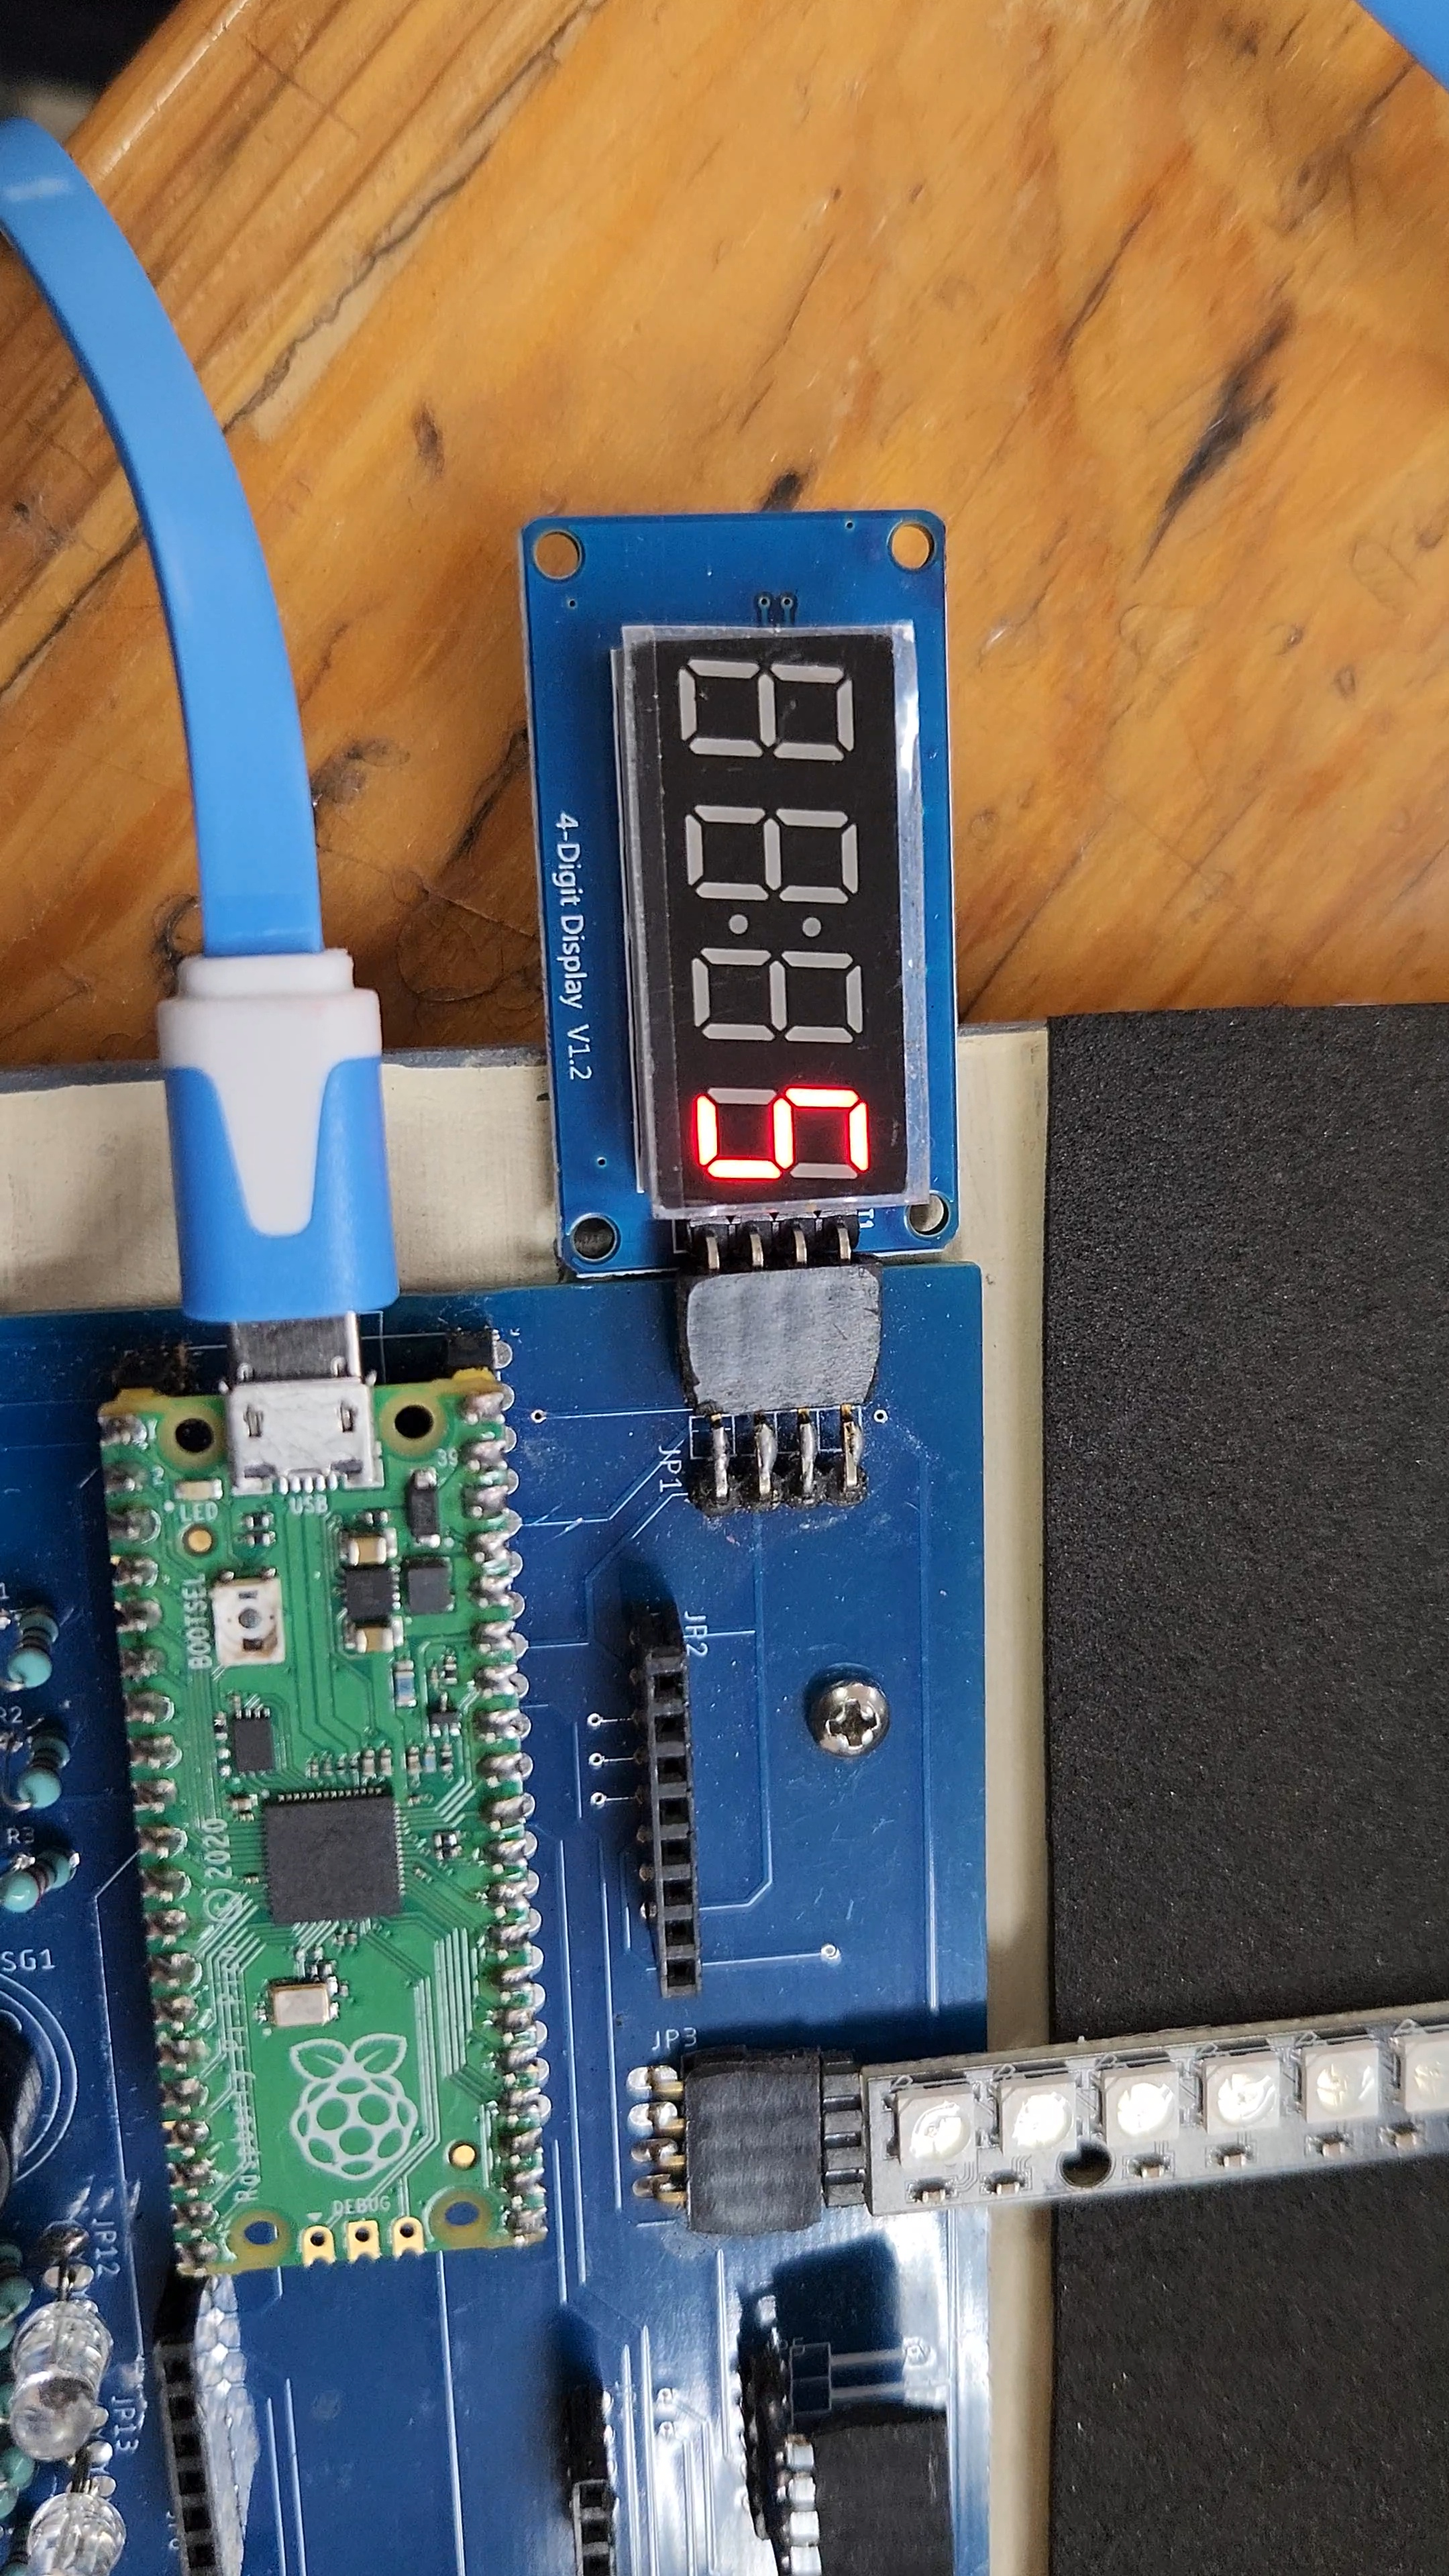
\includegraphics[width=0.6\textwidth, angle=90]{img/Actividad4/Act4_14.jpg}
        \caption{Valor 11}
    \end{minipage}
    \begin{minipage}{0.3\textwidth}
        \centering
        
\includegraphics[width=0.6\textwidth, angle=90]{img/Actividad4/Act4_2.jpg}
        \caption{Valor 10}
    \end{minipage}
    \begin{minipage}{0.3\textwidth}
        \centering
        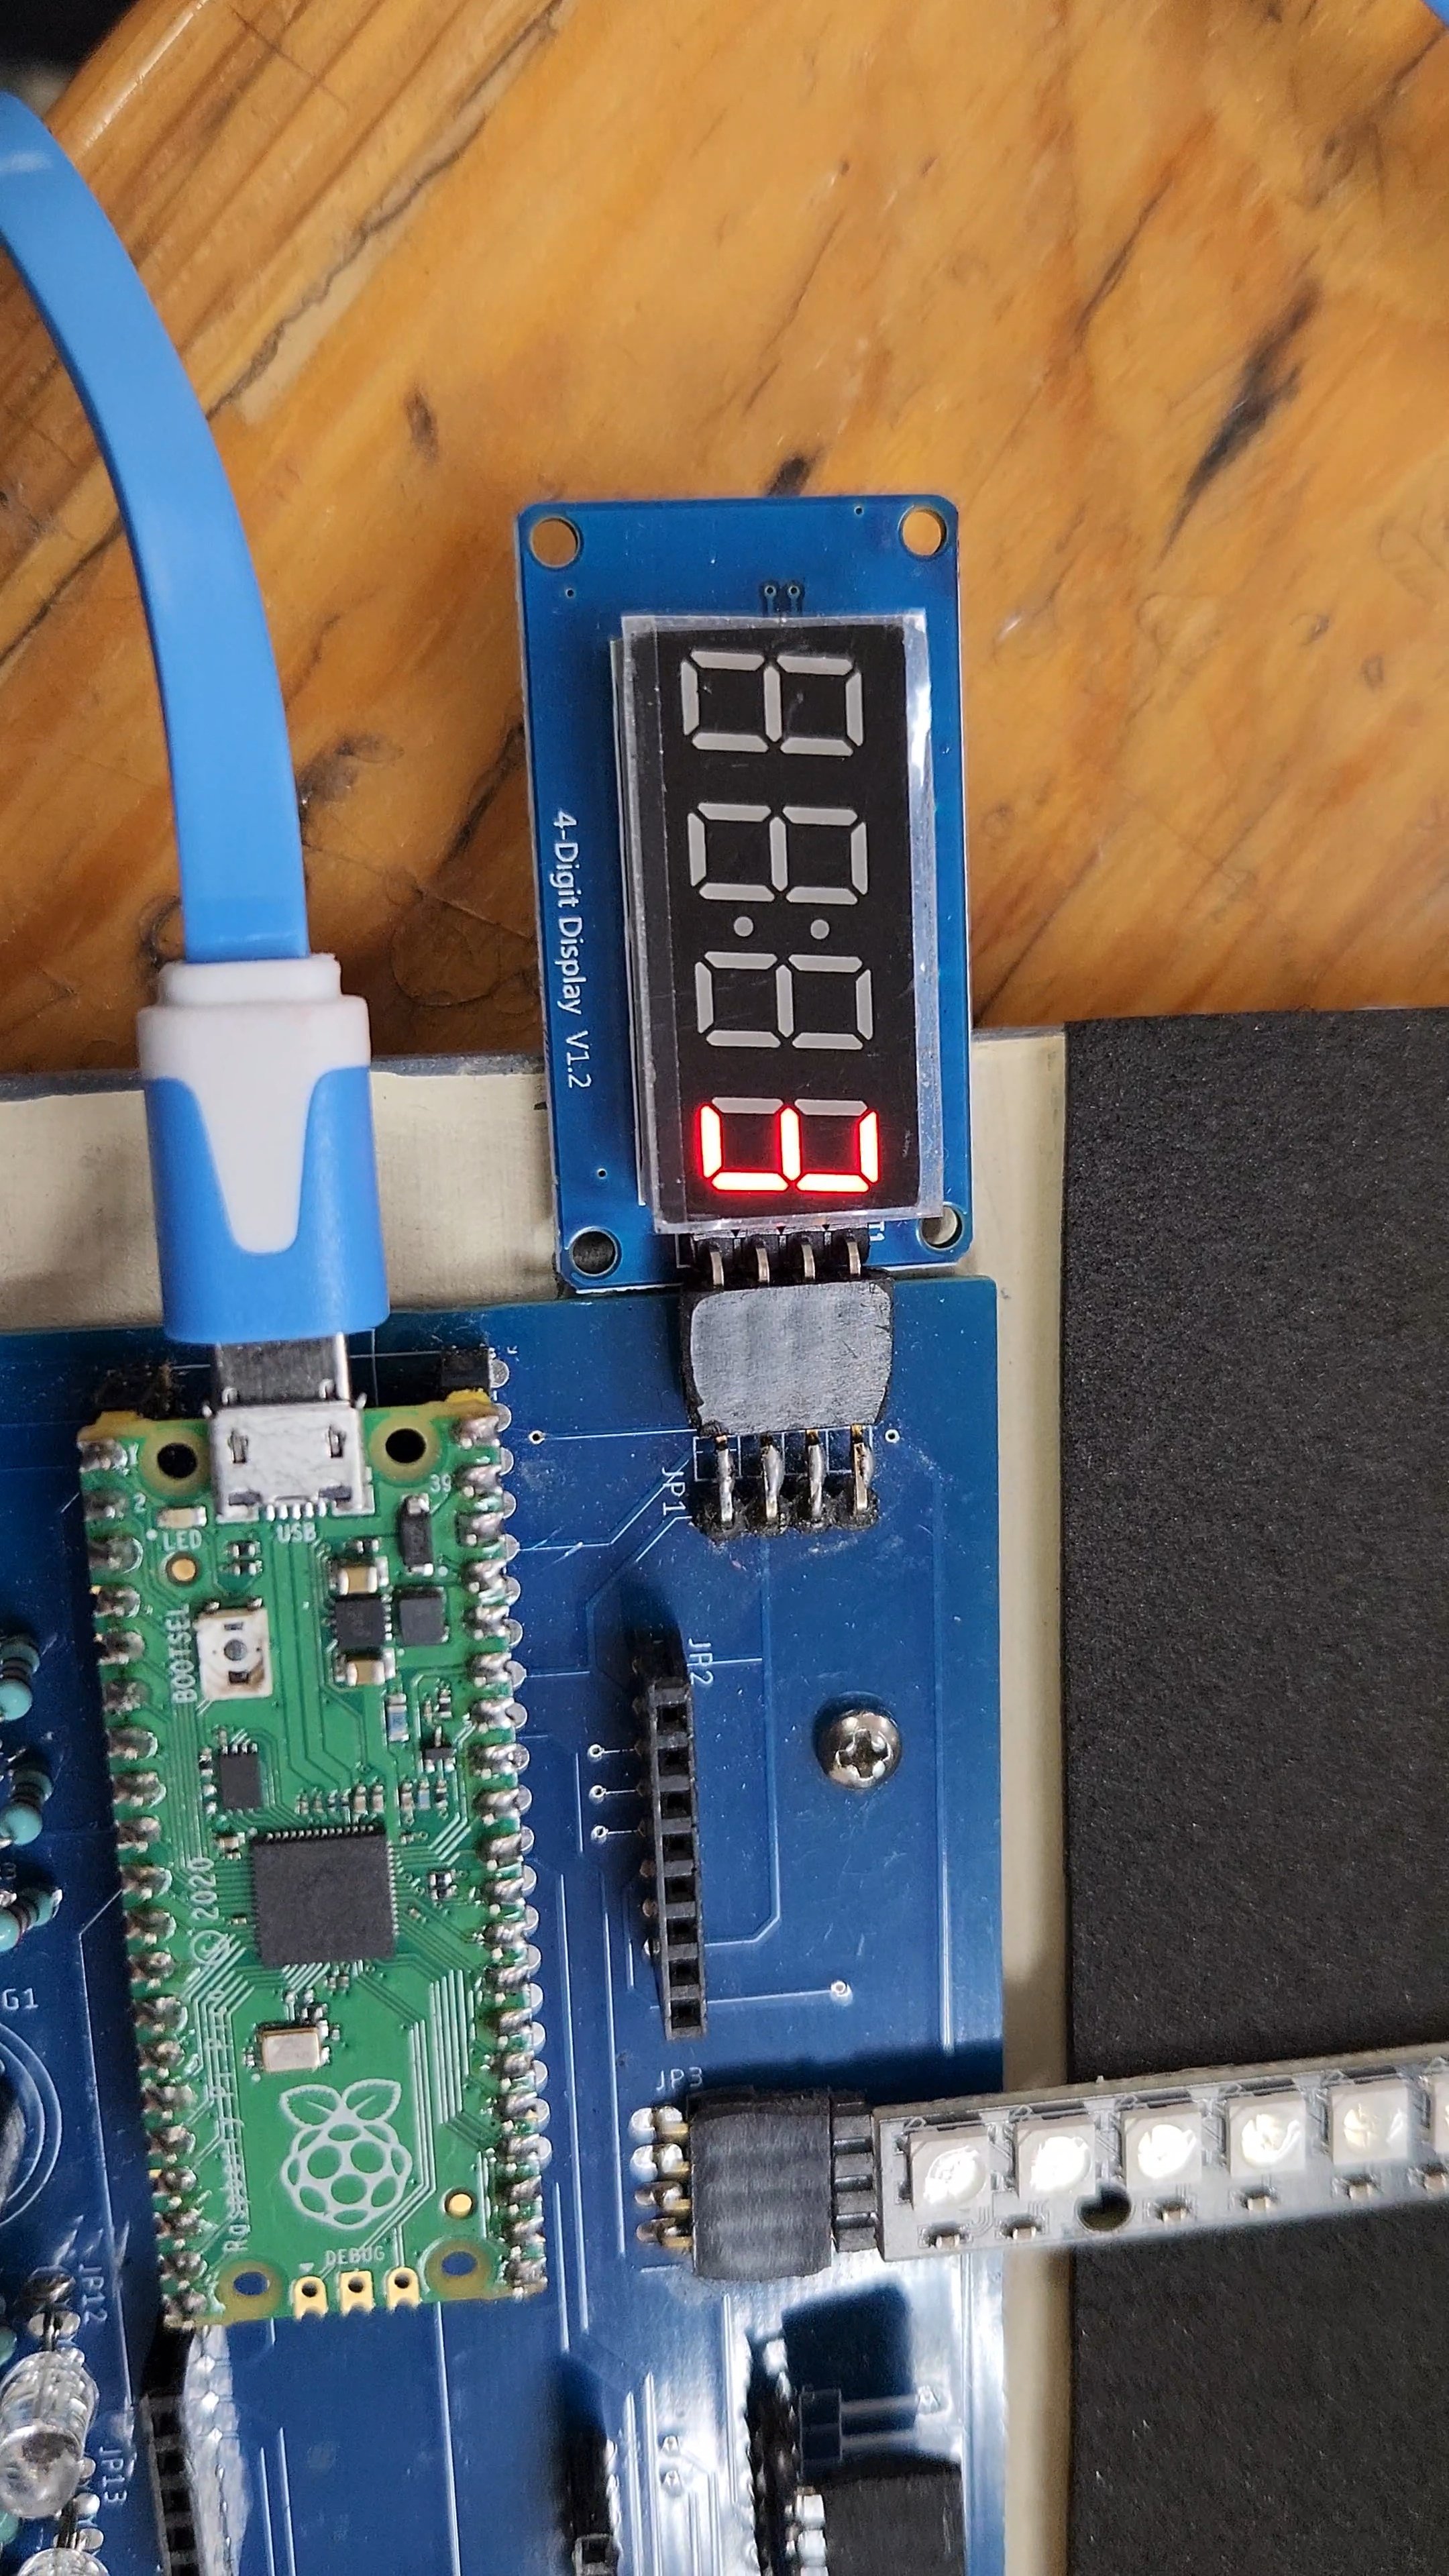
\includegraphics[width=0.6\textwidth, angle=90]{img/Actividad4/Act4_3.jpg}
        \caption{Valor 9}
    \end{minipage}
\end{figure}

\begin{figure}[H]
    \centering
    \begin{minipage}{0.3\textwidth}
        \centering
        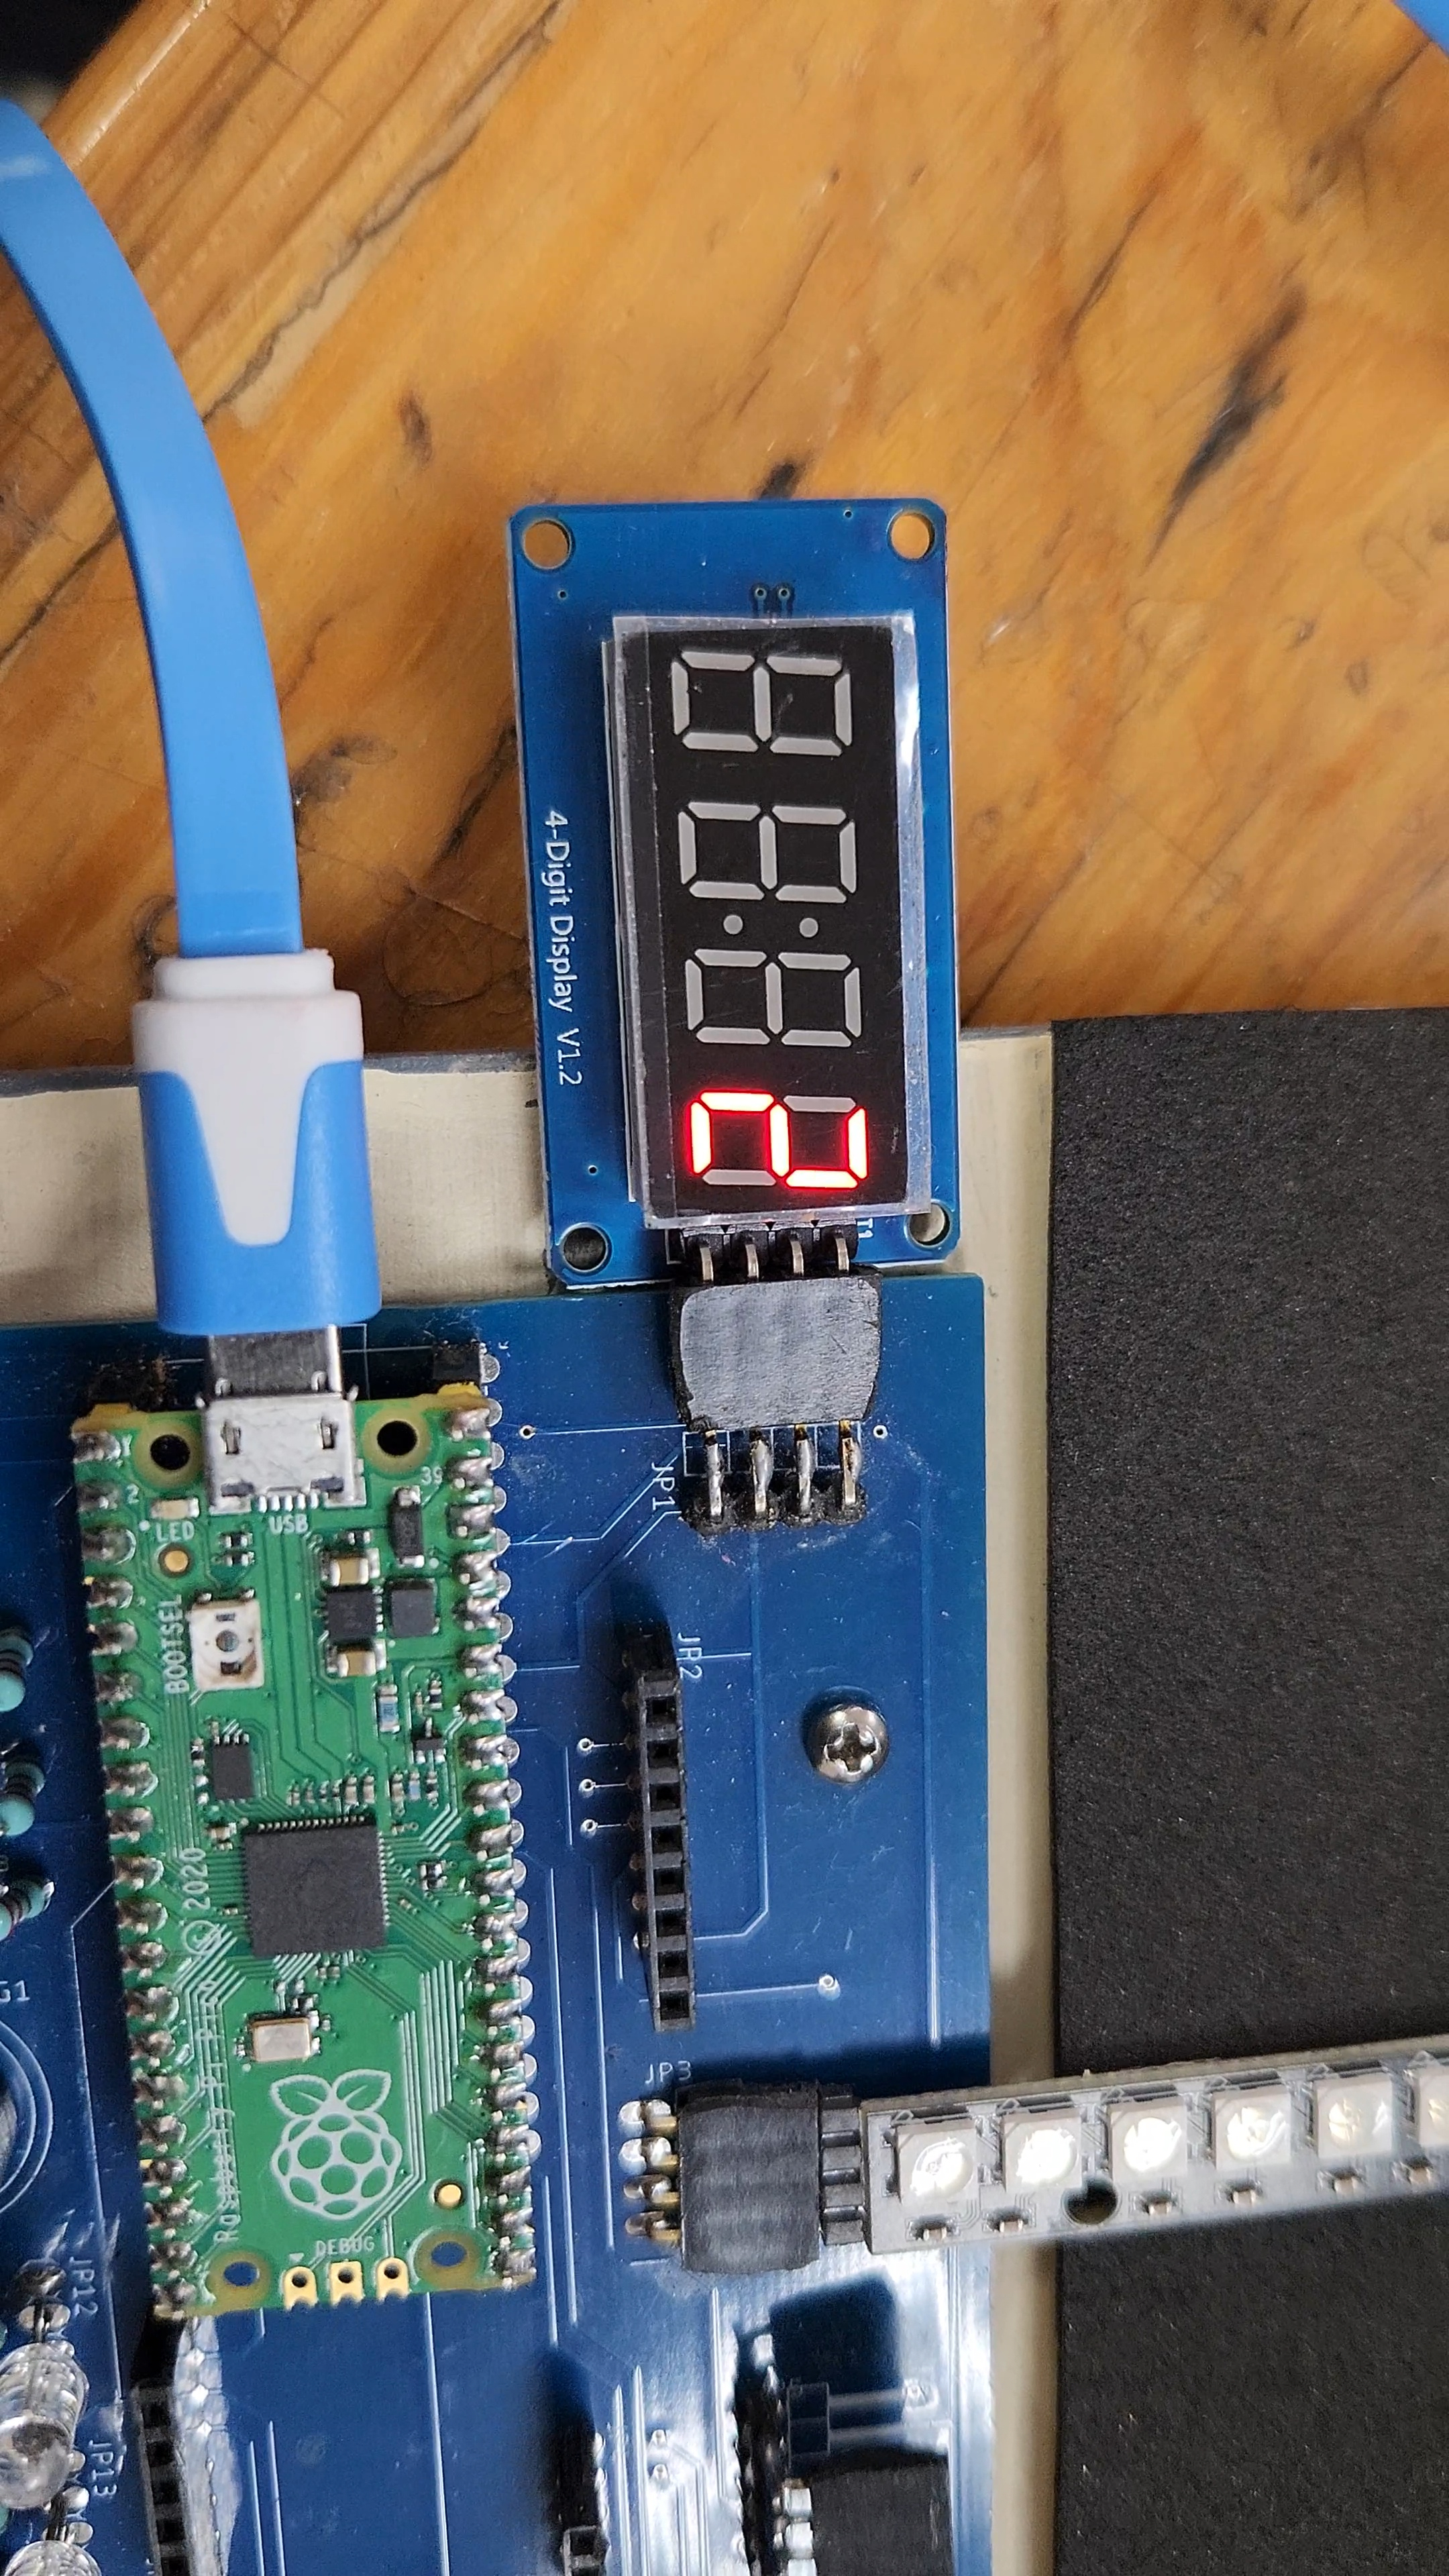
\includegraphics[width=0.6\textwidth, angle=90]{img/Actividad4/Act4_4.jpg}
        \caption{Valor 8}
    \end{minipage}
    \begin{minipage}{0.3\textwidth}
        \centering
        
\includegraphics[width=0.6\textwidth, angle=90]{img/Actividad4/Act4_5.jpg}
        \caption{Valor 7}
    \end{minipage}
    \begin{minipage}{0.3\textwidth}
        \centering
        
\includegraphics[width=0.6\textwidth, angle=90]{img/Actividad4/Act4_6.jpg}
        \caption{Valor 6}
    \end{minipage}
\end{figure}

\subsection*{Analisis de resultados}

El programa ejecuta correctamente el contador descendente desde 20 hasta 0, tal y como se obsevó en las figuras anteriores, cada valor se mostro en el display TM1637 con un intervalo de 1 segundo y al llegar a cero, el zumbador se activa durante 1 segundo emitiendo un tono audible. El uso del metodo \texttt{number()} simplifica el formateo de numeros hasta 4 digitos sin necesidad de gestionar manualmente los segmentos. El tiempo de espera de 1 segundo entre decrementos permite apreciar claramente cada valor antes de la siguiente actualizacion. La alarma al finalizar el conteo confirma visual y auditivamente la terminacion del proceso.
    \newpage
    \section*{Actividad 5}

    \noindent Escribir, comentar e indicar el funcionamiento del siguiente programa.

    \vspace{1.5cm}

    % Diagrama
    \begin{center}
    \begin{tikzpicture}
        % 1. Dibujar la Raspberry Pi Pico
        \picoboard

        % ==========================================
        % 2. Módulo Sensor DS18B20 (Lado Derecho)
        % ==========================================
        
        % Título sobre el sensor
        \node[align=left, font=\sffamily\small] at (9, -4.7) {Sensor de Temperatura\\[-0.1cm]DS18B20};

        % Contorno principal del sensor (caja gruesa)
        \draw[line width=2pt] (7.0, -5.5) rectangle (11.0, -9.5);
        
        % Texto grande dentro de la caja
        \node[font=\sffamily\small] at (9.3, -7.5) {DS18B20};

        % Etiquetas de los pines dentro de la caja
        \node[right, font=\sffamily\large] at (7.0, -6.5) {VDD};
        \node[right, font=\sffamily\large] at (7.0, -7.5) {DQ};
        \node[right, font=\sffamily\large] at (7.0, -8.5) {GND};

        % Terminales de los pines (líneas negras gruesas)
        \draw[line width=2.5pt] (7.0, -6.5) -- (6.2, -6.5); % Terminal VDD
        \draw[line width=2.5pt] (7.0, -7.5) -- (6.2, -7.5); % Terminal DQ
        \draw[line width=2.5pt] (7.0, -8.5) -- (6.2, -8.5); % Terminal GND

        % ==========================================
        % 3. Conexiones, Nodos Verdes y Símbolos
        % ==========================================

        % Cuadros verdes transparentes en los terminales del sensor
        \draw[green!80!black, thick, fill=green!20, opacity=0.8] (6.05, -6.35) rectangle (6.35, -6.65);
        \draw[green!80!black, thick, fill=green!20, opacity=0.8] (6.05, -7.35) rectangle (6.35, -7.65);
        \draw[green!80!black, thick, fill=green!20, opacity=0.8] (6.05, -8.35) rectangle (6.35, -8.65);

        % Conexión de alimentación VDD (3.3V)
        \draw[thick] (6.2, -6.5) -- (6.2, -5.6);
        \node[above, font=\sffamily\bfseries\small] at (6.2, -5.6) {3.3V};
        \draw[thick] (5.9, -5.6) -- (6.5, -5.6); % Base de la etiqueta 3.3V

        % Conexión GND
        \draw[thick] (6.2, -8.5) -- (6.2, -9.2);
        % Símbolo de GND (3 líneas horizontales)
        \draw[thick] (5.9, -9.2) -- (6.5, -9.2);
        \draw[thick] (6.0, -9.35) -- (6.4, -9.35);
        \draw[thick] (6.1, -9.5) -- (6.3, -9.5);

        % Conexión DQ (Cable Azul) hacia GP16 (Y = -9.0 en la Pico)
        % Se traza desde el extremo del terminal DQ hasta la salida de la Pico
        \draw[blue!80!cyan, thick] (6.2, -7.5) -- (4.4, -9.0);

    \end{tikzpicture}
    \end{center}

    \section*{Propuesta de solución}

    El código proporcionado implementa la lectura de temperatura utilizando el sensor digital DS18B20, que se comunica a través del protocolo 1-Wire. 

    De forma que lo primero que ser realiza en el programa es importar las librerías necesarias, entgre las librerías se encuentran \texttt{machine} para el control de pines y \texttt{onewire} para la comunicación 1-Wire, además de \texttt{ds18x20} que proporciona funciones específicas para interactuar con el sensor DS18B20, y por último \texttt{time} para gestionar los retardos necesarios.

    Ya con las librerías importadas, se configura el pin GPIO 16 como entrada/salida para la comunicación con el sensor. Luego, se crea una instancia del controlador DS18B20 utilizando la clase \texttt{DS18X20} donde el pin se especifica que utilice la capa OneWire \texttt{onewire.OneWire(ds\_pin)}.

    Como el sensor DS18B20 puede tener múltiples dispositivos conectados en paralelo, se realiza un escaneo del bus 1-Wire con el método \texttt{.scan()} para obtener las direcciones ROM únicas de cada sensor presente. De forma que en este caso se guarda unicamentela Rom de un solo sensor, al obener la dirección se imprinme en la consola para verificar la comunicación.

    Por medio de un bucle infinito, se crea el ciclo para leer y mostrar los datos del sensor de forma continua, para eso por medio del método \texttt{.convert\_temp()} se inicia la conversión de temperatura en el sensor, luego se espera un tiempo de 750 ms para asegurar que la conversión se complete. Posteriormente, se lee la temperatura en grados Celsius utilizando el método \texttt{.read\_temp(rom)}, ya con el valor númerico se procede a mostrat su contenido por medio de la impresión en consola, mostrando la dirección ROM del sensor y la temperatura en grados Celsius.

    \begin{figure}[H]
        \begin{tikzpicture}[
            node distance=1.35cm, scale=0.8,
            every node/.style={font=\small},
            % Definición de estilos para los bloques
            startstop/.style={rectangle, rounded corners, minimum width=3cm, minimum height=1cm, text centered, draw=black, fill=red!20},
            process/.style={rectangle, minimum width=3cm, minimum height=1cm, text centered, draw=black, fill=orange!20},
            decision/.style={diamond, aspect=2.2, minimum width=3cm, minimum height=1cm, text centered, draw=black, fill=green!20},
            arrow/.style={thick,->,>=stealth}
        ]

            % Nodos
            \node (start) [startstop, text width=3.2cm] {Inicio};
            
            \node (init) [process, below=of start, text width=8.6cm] {Configurar GPIO16, instanciar \texttt{ds\_sensor} en bus 1-Wire.};
            
            \node (scan) [process, below=of init, text width=8.6cm] {Ejecutar \texttt{roms = ds\_sensor.scan()} e imprimir "Sensor detectado".};
            
            \node (conv) [process, below=of scan, text width=7.0cm] {Iniciar conversión con \texttt{convert\_temp()}.};
            
            \node (wait) [process, below=of conv, text width=7.0cm] {Esperar 750 ms (\texttt{time.sleep\_ms(750)}).};
            
            \node (for) [decision, below=of wait, text width=4.0cm, aspect=2.2] {\texttt{for rom in roms}:\newline \textquestiondown Hay ROM pendiente?};
            
            \node (read) [process, below=of for, text width=8.0cm] {Imprimir \texttt{ROM}, leer \texttt{tempC} e imprimir temperatura formateada.};
            
            \node (pause) [process, right=2cm of for, text width=3.2cm, align=center] {Esperar 2 s (\texttt{time.sleep(2)}).};

            % Conexiones (Flechas)
            \draw [arrow] (start) -- (init);
            \draw [arrow] (init) -- (scan);
            \draw [arrow] (scan) -- (conv);
            
            % Bucle While (Implícito en la repetición hacia conv)
            \draw [arrow] (conv) -- (wait);
            \draw [arrow] (wait) -- (for);
            
            % Bucle For - Ruta Verdadera (Sí hay sensor pendiente)
            \draw [arrow] (for) -- node[right, font=\scriptsize] {Sí} (read);
            % Retorno del Bucle For (Sube nuevamente para la evaluación)
            \draw [arrow] (read.west) -- ++(-2.8,0) |- (for.west);
            
            % Bucle For - Ruta Falsa (Fin del iterador For, pasa a la pausa del While)
            \draw [arrow] (for.east) -- node[above, font=\scriptsize] {No} (pause.west);
            
            % Retorno del Bucle While (Regresa al inicio de la conversión después de la pausa)
            \draw [arrow] (pause.north) |- (conv.east);

        \end{tikzpicture}
        \centering
        \caption{Diagrama de Flujo: Actividad 5}
    \end{figure}

    \newpage

    \section*{Desarrollo}

    \lstinputlisting[language={[LAB]Python}, caption=Código de la Actividad 5, basicstyle=\ttfamily\scriptsize]{Code/Act5.py}

    \begin{figure}[H]
        \centering
        
\includegraphics[width=0.9\textwidth]{img/Actividad5/Act5_1.jpg}
        \caption{Actividad 5. Impresión de la dirección ROM del sensor y la temperatura en grados Celsius en un primer insante de tiempo.}
    \end{figure}

    \begin{figure}[H]
        \centering
        
\includegraphics[width=0.9\textwidth]{img/Actividad5/Act5_2.jpg}
        \caption{Actividad 5. Impresión de la dirección ROM del sensor y la temperatura en grados Celsius en un segundo insante de tiempo.}
    \end{figure}

    \subsection*{Análisis de resultados}

    A partir de las imagenes obtenidas al ejecutar el programa en la placa de desarrollo Raspberry Pi Pico, se puede observar que el microcontrolador logra establecer comunicación con el sensor DS18B20, detectando su presencia y obteniendo su dirección ROM única, lo que confirma que la capa de comunicación 1-Wire está funcionando correctamente. Además, el programa es capaz de iniciar la conversión de temperatura, esperar el tiempo necesario para que el sensor complete su medición, y luego leer e imprimir la temperatura en grados Celsius con un formato adecuado. De forma que el programa logra medir la temperatura usando el sensor DS18B20 y el protocolo 1-Wire, mostrando los resultados en la consola de manera continua cada 2 segundos.

    \newpage
    \section*{Actividad 6}

    \noindent Realizar las modificaciones necesarias al programa anterior, para mostrar también la temperatura en $^\circ$F.

    \vspace{1cm}

    % ==========================================
    % Bloque de salida de consola/código
    % ==========================================
    \begin{center}
        % Usamos un minipage para agrupar el texto y centrar el bloque entero
        \begin{minipage}{0.65\textwidth}
            \ttfamily % Cambia la fuente a monoespaciada (tipo consola)
            bytearray(b' (\textbackslash x0f\textbackslash x95D\textbackslash xd4\textbackslash xe1<\textbackslash x9a')\\
            temperature ($^\circ$C): 23.56\\
            temperature ($^\circ$F): 74.41\\[0.5cm]
            bytearray(b' (\textbackslash x0f\textbackslash x95D\textbackslash xd4\textbackslash xe1<\textbackslash x9a')\\
            temperature ($^\circ$C): 23.56\\
            temperature ($^\circ$F): 74.41
        \end{minipage}
        
        \vspace{0.8cm}
        
        % Pie de figura
        {\sffamily Figura 9-15. Temperatura con DS18B20 en $^\circ$C y $^\circ$F}
    \end{center}    

    \section*{Propuesta de solución}
    Para leer la temperatura ambiental con alta precisión, se propone implementar la comunicación mediante el protocolo \textit{1-Wire} (un solo hilo) exigido por el sensor digital DS18B20. Haciendo uso de las librerías \texttt{onewire} y \texttt{ds18x20}, el algoritmo escanea inicialmente el bus de datos en el GPIO 16 para detectar e identificar las direcciones ROM únicas de todos los dispositivos conectados en paralelo.

    Dentro del ciclo continuo, se envía un comando global para iniciar la conversión térmica. Se debe aplicar un retardo estricto de 750 milisegundos para permitir que el convertidor analógico-digital interno del sensor finalice su cálculo. Posteriormente, se extrae el dato crudo en grados Celsius. A través de una operación aritmética simple, este valor se convierte a grados Fahrenheit. Finalmente, el microcontrolador formatea e imprime en la consola tanto la dirección física del dispositivo como las dos magnitudes de temperatura resultantes.

\begin{center}
    \begin{tikzpicture}[node distance=1.35cm, every node/.style={font=\small}]
        \node (start6) [startstop, text width=3.2cm] {Inicio};
        \node (init6) [process, below=of start6, text width=8.6cm] {Importar modulos, crear \texttt{ds\_sensor} en GPIO16 y ejecutar \texttt{roms = ds\_sensor.scan()}.};
        \node (conv6) [process, below=of init6, text width=7.0cm] {Iniciar conversion con \texttt{convert\_temp()}.};
        \node (wait6) [process, below=of conv6, text width=7.0cm] {Esperar 750 ms para completar conversion.};
        \node (for6) [decision, below=of wait6, text width=4.0cm, aspect=2.2] {\texttt{for rom in roms}:\newline \textquestiondown Hay ROM pendiente?};
        \node (read6) [process, below=of for6, text width=8.0cm] {Leer \texttt{tempC = read\_temp(rom)} y calcular \texttt{tempF = tempC*9/5 + 32}.};
        \node (print6) [process, below=of read6, text width=8.0cm] {Imprimir \texttt{ROM}, temperatura en \textdegree C y en \textdegree F.};
        
        % CORRECCIÓN: Se cambió "below=of" por "right=2cm of" para mover el bloque a la derecha
        \node (pause6) [process, right=2cm of for6, text width=3.2cm, align=center] {Esperar 2 s.};

        \draw [arrow] (start6) -- (init6);
        \draw [arrow] (init6) -- (conv6);
        \draw [arrow] (conv6) -- (wait6);
        \draw [arrow] (wait6) -- (for6);
        \draw [arrow] (for6) -- node[right, font=\scriptsize] {Si} (read6);
        \draw [arrow] (read6) -- (print6);
        \draw [arrow] (print6.west) -- ++(-2.8,0) |- (for6.west);
        
        % CORRECCIÓN: La flecha sale por el este hacia el oeste de la pausa
        \draw [arrow] (for6.east) -- node[above, font=\scriptsize] {No} (pause6.west);
        
        % CORRECCIÓN: La flecha sube desde el norte de la pausa y entra por el este a la conversión
        \draw [arrow] (pause6.north) |- (conv6.east);
    \end{tikzpicture}
    \end{center}

    El flujo de datos parte de la deteccion inicial de direcciones ROM en el bus 1-Wire y luego entra al ciclo principal de conversion termica. En cada vuelta se genera una conversion global, se espera el tiempo fisico del sensor y se recorre la lista \texttt{roms}; por cada direccion se extrae \texttt{tempC}, se transforma a \texttt{tempF} y ambas magnitudes se envian a salida serial junto con la ROM que identifica al dispositivo. Cuando termina el recorrido de sensores, el programa aplica una pausa de 2 segundos y reinicia el proceso de muestreo.

    \section*{Desarrollo}

    \lstinputlisting[language={[LAB]Python}, caption=Código de la Actividad 6, basicstyle=\ttfamily\scriptsize]{Code/Act6.py}

    \begin{figure}[H]
        \centering
        
\includegraphics[width=0.9\textwidth]{img/Actividad6/Act6_1.jpg}
        \caption{Identificación y respuesta térmica inicial. }
    \end{figure}

    \begin{figure}[H]
        \centering
        
\includegraphics[width=0.9\textwidth]{img/Actividad6/Act6_2.jpg}
        \caption{Pico térmico y disipación de calor. En las iteraciones posteriores, el sistema registra un máximo térmico sostenido de 32.50 °C seguido de una caída a 31.56 °C. Este registro demuestra que el ciclo de muestreo captura fielmente la inercia térmica y el enfriamiento natural del componente físico en tiempo real, garantizando lecturas estables tras el tiempo de conversión de 750 ms.}
    \end{figure}

    \subsection*{Análisis de resultados}
    El script demuestra un control sólido sobre el protocolo bidireccional de un solo hilo. La instrucción \texttt{ds\_sensor.scan()} localiza físicamente el sensor y devuelve su dirección inalterable de fábrica en un arreglo de bytes (\texttt{bytearray}), el cual coincide exactamente con la salida observada en el monitor serial. Esto asegura que los comandos posteriores se dirijan al hardware correcto.

    La ejecución de \texttt{ds\_sensor.convert\_temp()} ordena al DS18B20 tomar una muestra del entorno. El retardo de 750 ms resulta crítico en esta etapa, ya que es el tiempo físico que tarda el sensor en procesar la temperatura con su máxima resolución de 12 bits. Una vez extraído el valor con \texttt{read\_temp()}, el procesador aplica la conversión (\texttt{tempC * 9/5 + 32}). Los resultados impresos en la consola, como los 23.56 °C y 74.41 °F, muestran una lectura térmica estable, validando la inmunidad al ruido eléctrico que ofrece este sensor digital frente a los sensores analógicos de las prácticas anteriores.

    \newpage
    \section*{Actividad 7}

    \noindent  Escribir, comentar e indicar el funcionamiento del siguiente programa; estudiar la librería usada.

    \vspace{1.5cm}

    % Diagrama
    \begin{center}
    \begin{tikzpicture}
        % 1. Dibujar la Raspberry Pi Pico
        \picoboard

        % ==========================================
        % 2. Módulo Sensor DTH11 (Lado Derecho)
        % ==========================================
        
        % Título flotante sobre el sensor
        \node[align=center, text=blue!60!black, font=\sffamily\bfseries\itshape\small] at (8.5, -4.0) {Sensor de\\[0.1cm]Temperatura\\[0.1cm]y Humedad\\[0.1cm]DTH11};

        % Contorno del sensor (rectángulo)
        \draw[thick] (6.5, -5.3) rectangle (8.5, -7.3);
        
        % Conexión S (Cable azul) hacia GP21 (Y = -6.3 en la Pico)
        \draw[blue!80!cyan, thick] (6.5, -6.3) -- (4.4, -6.3);
        % Letra 'S' al interior del borde
        \node[right, font=\sffamily\bfseries\large, inner sep=3pt] at (6.5, -6.3) {S};

        % Conexión VCC (Cable rojo superior)
        \draw[red, thick] (6.8, -5.3) -- (6.8, -4.6);
        % Etiqueta VCC al lado del cable
        \node[left, font=\sffamily\bfseries\large, inner sep=4pt] at (6.8, -4.95) {VCC};
        % Indicador de 3.3V
        \node[above, font=\sffamily\bfseries\small] at (6.8, -4.6) {3.3V};
        \draw[thick] (6.5, -4.6) -- (7.1, -4.6); % Línea base de 3.3V

        % Conexión GND (Cable inferior negro)
        \draw[thick] (6.8, -7.3) -- (6.8, -8.0);
        % Etiqueta GND al lado del cable
        \node[left, font=\sffamily\bfseries\large, inner sep=4pt] at (6.8, -7.65) {GND};
        
        % Símbolo de GND (3 líneas horizontales verdes)
        \draw[green!70!black, thick] (6.5, -8.0) -- (7.1, -8.0);
        \draw[green!70!black, thick] (6.65, -8.15) -- (6.95, -8.15);
        \draw[green!70!black, thick] (6.75, -8.3) -- (6.85, -8.3);

    \end{tikzpicture}
    \end{center}

    \section*{Propuesta de solución}

    El código proporcionado corresponde a la implementación de un programa para medir la temperatura y humedad utilizando el sensor DTH11. Debiodo a esto la inicio del programa se realiza la imporación de bibliotecas necearias para su correcto funcionamiento.

    Las bibliotecas que se utilizan son el módulo \texttt{dht} para poder realizar la comunicaciín con el sensor \texttt{DHT}, es importante destcar que este sensor emplea un protocolo de comunicación del tipo propiietario, de forma que a diferencia del protocolo one-wire del DS18B20, el DHT11 requiere una secuencia específica de señales para iniciar la comunicación y obtener los datos de temperatura y humedad. Por otro lado se reliza la imporación de la biblioteca \texttt{machine} para el control de los pines GPIO, y por último se importa la biblioteca \texttt{time} para gestionar los retardos necesarios en la comunicación con el sensor.

    Por medio mde un ciclo infinito se realiza la lectura, para solicitar los datos correspondientes al sensor, port medio del método \texttt{dht11.measure()} se inicia la comunicación con el sensor, obteniendo una trama de datos de 40 bits que contiene la información de temperatura y humedad. Luego se extraen los valores de temperatura y humedad utilizando las propiedades \texttt{dht11.temperature()} y \texttt{dht11.humidity()}, respectivamente. Ya con los valores obtenidos se procede a imprimir en la consola la temperatura en grados Celsius y la humedad relativa en porcentaje, con un formato claro y legible. Este programa implementa un bloque try-catch para manejar posibles errores de comunicación con el sensor, como lecturas fallidas o desconexiones, lo que garantiza que el programa no se detenga abruptamente ante una falla en la lectura del DHT11.

    \begin{figure}[H]
        \begin{tikzpicture}[
            node distance=1.5cm, 
            every node/.style={font=\small},
            % Estilos de los bloques
            startstop/.style={rectangle, rounded corners, minimum width=3cm, minimum height=1cm, text centered, draw=black, fill=red!20},
            process/.style={rectangle, minimum width=3cm, minimum height=1cm, text centered, draw=black, fill=orange!20},
            decision/.style={diamond, aspect=2, minimum width=3cm, minimum height=1cm, text centered, draw=black, fill=green!20},
            arrow/.style={thick,->,>=stealth}
        ]

            % Nodos
            \node (start) [startstop] {Inicio};
            
            \node (init) [process, below=of start, text width=6cm] {Configurar DHT11 en GPIO 21 (\texttt{Sensor = dht.DHT11(...)}).};
            
            \node (measure) [process, below=of init, text width=5cm] {Solicitar medición (\texttt{Sensor.measure()}).};
            
            \node (check) [decision, below=of measure, text width=3.5cm] {¿Ocurrió un \texttt{OSError}?};
            
            \node (success) [process, below=of check, text width=6cm] {Leer \texttt{temp}, \texttt{hum} e imprimir: \enquote{Temperatura: ... Humedad: ...}};
            
            \node (error) [process, right=1.5cm of check, text width=4cm] {Imprimir: \enquote{Fallo de sincronización, reintentando...}};
            
            \node (sleep) [process, below=of success, text width=4cm] {Esperar 2 s (\texttt{time.sleep(2)}).};

            % Conexiones (Flechas)
            \draw [arrow] (start) -- (init);
            \draw [arrow] (init) -- (measure);
            \draw [arrow] (measure) -- (check);
            
            % Ruta sin error (Try exitoso)
            \draw [arrow] (check) -- node[right, font=\scriptsize] {No} (success);
            
            % Ruta con error (Except OSError)
            \draw [arrow] (check) -- node[above, font=\scriptsize] {Sí} (error);
            
            % Ambas rutas convergen en la pausa de 2 segundos
            \draw [arrow] (success) -- (sleep);
            \draw [arrow] (error.south) |- (sleep.east);
            
            % Retorno del Bucle While (Vuelve a solicitar la medición)
            \draw [arrow] (sleep.west) -- ++(-2.5,0) |- (measure.west);
        \end{tikzpicture}
        \centering
        \caption{Diagrama de Flujo: Actividad 7}
    \end{figure}


    \section*{Desarrollo}

    \lstinputlisting[language={[LAB]Python}, caption=Código de la Actividad 7, basicstyle=\ttfamily\scriptsize]{Code/Act7.py}
    
    \begin{figure}[H]
        \centering
        
\includegraphics[width=0.9\textwidth]{img/Actividad7/Act7_1.jpg}
        \caption{Actividad 7. Impresión de datos de Temperatura y Humedad.}
    \end{figure}
    
    \newpage
    
    \subsection*{Análisis de resultados}
    Al ejecutar el programa en la Raspberry Pi Pico, se puede verificar que el programa funciona correctamente ya que en la consola se imprime de formna correcta la temperatura en grados Celsius y la humedad relativa en porcentaje, con un formato claro y legible. De forma que para verificar que el sensor DHT11 se encuentra en funcionando de fornma correcta, para esto se vario el ambiente del sensor, por ejemplo al colocar la mano sobre el sensor se puede observar un incremento en la temperatura y humedad relativa, lo que confirma que el programa logra medir correctamente la temperatura y humedad utilizando el sensor DHT11. Al poder recuperar los datos de temperatura y humedad se puede concluir que se realizo de forma correcta la comunicación con el sensor, y que el programa es capaz de manejar posibles errores de comunicación, como lecturas fallidas o desconexiones, lo que garantiza que el programa no se detenga abruptamente ante una falla en la lectura del DHT11.

    \newpage
    \section*{Actividad 8}

    \noindent  Utilizando el sensor DTH11, modificar el programa anterior, para que indique el momento en que se ha incrementado la temperatura de referencia, en la cercanía del sensor en razón de 5 $^\circ$C \textit{(temperatura tomada de la actividad anterior)}, como se indica en la tabla 9-1.

    \vspace{1cm}

    % ==========================================
    % Tabla
    % ==========================================
    \begin{center}
        % Configuración de las líneas de la tabla
        \setlength{\arrayrulewidth}{0.5pt} % Grosor de la línea
        \arrayrulecolor{BorderBlue}        % Color de las líneas de la tabla
        \renewcommand{\arraystretch}{1.5}  % Espaciado vertical para que no se vea apretada

        \begin{tabular}{|c|c|c|}
            \hline
            % Fila de Encabezado
            \rowcolor{HeaderBlue}
            \textcolor{white}{\textbf{\textsf{Temperatura DTH11}}} & 
            \textcolor{white}{\textbf{\textsf{LED (GPIO20)}}} & 
            \textcolor{white}{\textbf{\textsf{Zumbador (GPIO17)}}} \\
            \hline
            
            % Fila 1 (Fondo azul claro)
            \rowcolor{RowBlue}
            \textbf{Temp\_actual $\leq$ Temp\_ref + 5$^\circ$C} & 0 & 0 \\
            \hline
            
            % Fila 2 (Fondo blanco por defecto)
            \textbf{Temp\_actual $>$ Temp\_ref + 5$^\circ$C} & 1 & 1 \\
            \hline
        \end{tabular}

        \vspace{0.5cm}
        % Pie de tabla
        {\sffamily Tabla 9-1. Control; actividad 8}
    \end{center}

    \section*{Propuesta de solución}

    Para poder impolementar el programa que controle el funcionamiento de un LED y un zumbador en función de la temperatura medida por el sensor DHT11, se propone seguir los siguientes pasos:

    Dado que se va a medir la temperatura usando el sensor DHT11, se seberealizar la importacón de las bibliotecas necesarias, entre las cuales se encuentran el módulo \texttt{dht} para la comunicación con el sensor DHT11, el módulo \texttt{machine} para el control de los pines GPIO, y el módulo \texttt{time} para gestionar los retardos necesarios.

    Ya con las dependencias configuradas, se procede a instanciar una objeto del sensor DHT11 en el pin GPIO 21, y se configuran los pines GPIO 20 y GPIO 17 como salidas para controlar el LED y el zumbador, respectivamente. Posteriorment se define una variable de referencia para la temperatura, que se puede establecer a partir de una lectura previa del sensor o un valor fijo.

    De igual igual forma que en implementaciones anteriores, se crea un ciclo infinito para realizar la lectura continua de la temperatura y humedad. Dentro del ciclo, se solicita una medición al sensor DHT11 y se extraen los valores de temperatura y humedad, y estos se muestran ppor medio de la consola, posteriormente se compara la temperatura actual con la temperatura de referencia más un margen de 5 °C. Si la temperatura actual supera este umbral, se enciende el LED y el zumbador; de lo contrario, ambos dispositivos permanecen apagados. Finalmente, se imprime en la consola la temperatura actual y se aplica una pausa de 2 segundos antes de la siguiente lectura.

    \begin{figure}[H]
        \begin{tikzpicture}[
            node distance=0.7cm, scale=0.5,
            every node/.style={font=\small},
            % Estilos de los bloques
            startstop/.style={rectangle, rounded corners, minimum width=3cm, minimum height=1cm, text centered, draw=black, fill=red!20},
            process/.style={rectangle, minimum width=3cm, minimum height=1cm, text centered, draw=black, fill=orange!20},
            decision/.style={diamond, aspect=2, minimum width=3cm, minimum height=1cm, text centered, draw=black, fill=green!20},
            arrow/.style={thick,->,>=stealth}
        ]

            % Nodos Principales
            \node (start) [startstop] {Inicio};
            
            \node (init) [process, below=of start, text width=7.5cm] {Configurar DHT11 (GPIO21), LED (GPIO20), Buzzer (GPIO17) y \texttt{Temp\_ref = 25}.};
            
            \node (measure) [process, below=of init, text width=5cm] {Solicitar medición (\texttt{Sensor.measure()}).};
            
            % Nodo de Decisión de Error
            \node (check_error) [decision, below=of measure, text width=3.5cm] {¿\texttt{OSError}?};
            
            % Ruta de Error (Hacia la izquierda)
            \node (error_msg) [process, left=1cm of check_error, text width=3cm] {Imprimir error.};
            
            % Ruta Normal (Continuación hacia abajo)
            \node (read_temp) [process, below=of check_error, text width=6cm] {Leer \texttt{Temp\_actual} e imprimir estado contra el umbral.};
            
            % Nodo de Decisión de Temperatura
            \node (check_temp) [decision, below=of read_temp, text width=4.5cm] {¿\texttt{Temp\_actual} > \texttt{Temp\_ref} + 5?};
            
            % Acciones del Umbral
            \node (alarm_on) [process, right=1.5cm of check_temp, text width=3cm] {Activar alarmas:\\\texttt{led.value(1)}\\\texttt{buzzer.value(1)}};
            \node (alarm_off) [process, below=of check_temp, text width=3cm] {Apagar alarmas:\\\texttt{led.value(0)}\\\texttt{buzzer.value(0)}};
            
            % Pausa final
            \node (sleep) [process, below=of alarm_off, text width=4cm] {Esperar 2 s (\texttt{time.sleep(2)}).};

            % Conexiones Directas
            \draw [arrow] (start) -- (init);
            \draw [arrow] (init) -- (measure);
            \draw [arrow] (measure) -- (check_error);
            
            % Conexiones del Check Error
            \draw [arrow] (check_error) -- node[above, font=\scriptsize] {Sí} (error_msg);
            \draw [arrow] (check_error) -- node[right, font=\scriptsize] {No} (read_temp);
            
            % Conexiones del Check Temp
            \draw [arrow] (read_temp) -- (check_temp);
            \draw [arrow] (check_temp) -- node[above, font=\scriptsize] {Sí} (alarm_on);
            \draw [arrow] (check_temp) -- node[right, font=\scriptsize] {No} (alarm_off);
            
            % Convergencia hacia Sleep
            \draw [arrow] (alarm_off) -- (sleep);
            \draw [arrow] (alarm_on.south) |- (sleep.east);
            \draw [arrow] (error_msg.south) |- (sleep.west);
            
            % Bucle While (Retorno seguro)
            % Creamos una coordenada invisible a la izquierda del bloque de error para que la línea no lo corte
            \path (error_msg.west) -- ++(-1.5,0) coordinate (loop_left);
            % Trazamos la línea desde abajo de 'sleep', pasamos por 'loop_left' y subimos a 'measure'
            \draw [arrow] (sleep.south) -- ++(0,-0.5) -| (loop_left) |- (measure.west);

        \end{tikzpicture}
        \centering
        \caption{Diagrama de Flujo: Actividad 8}
    \end{figure}
    

    \section*{Desarrollo}

    \lstinputlisting[language={[LAB]Python}, caption=Código de la Actividad 8, basicstyle=\ttfamily\scriptsize]{Code/Act8.py}

        \begin{figure}[H]
            \centering
            
\includegraphics[width=0.75\textwidth]{img/Actividad8/Act8_1.jpg}
            \caption{Actividad 8. Medición de temperatura actual y comparación con el umbral de referencia en un primer instante de tiempo.}
        \end{figure}

        \begin{figure}[H]
            \centering
            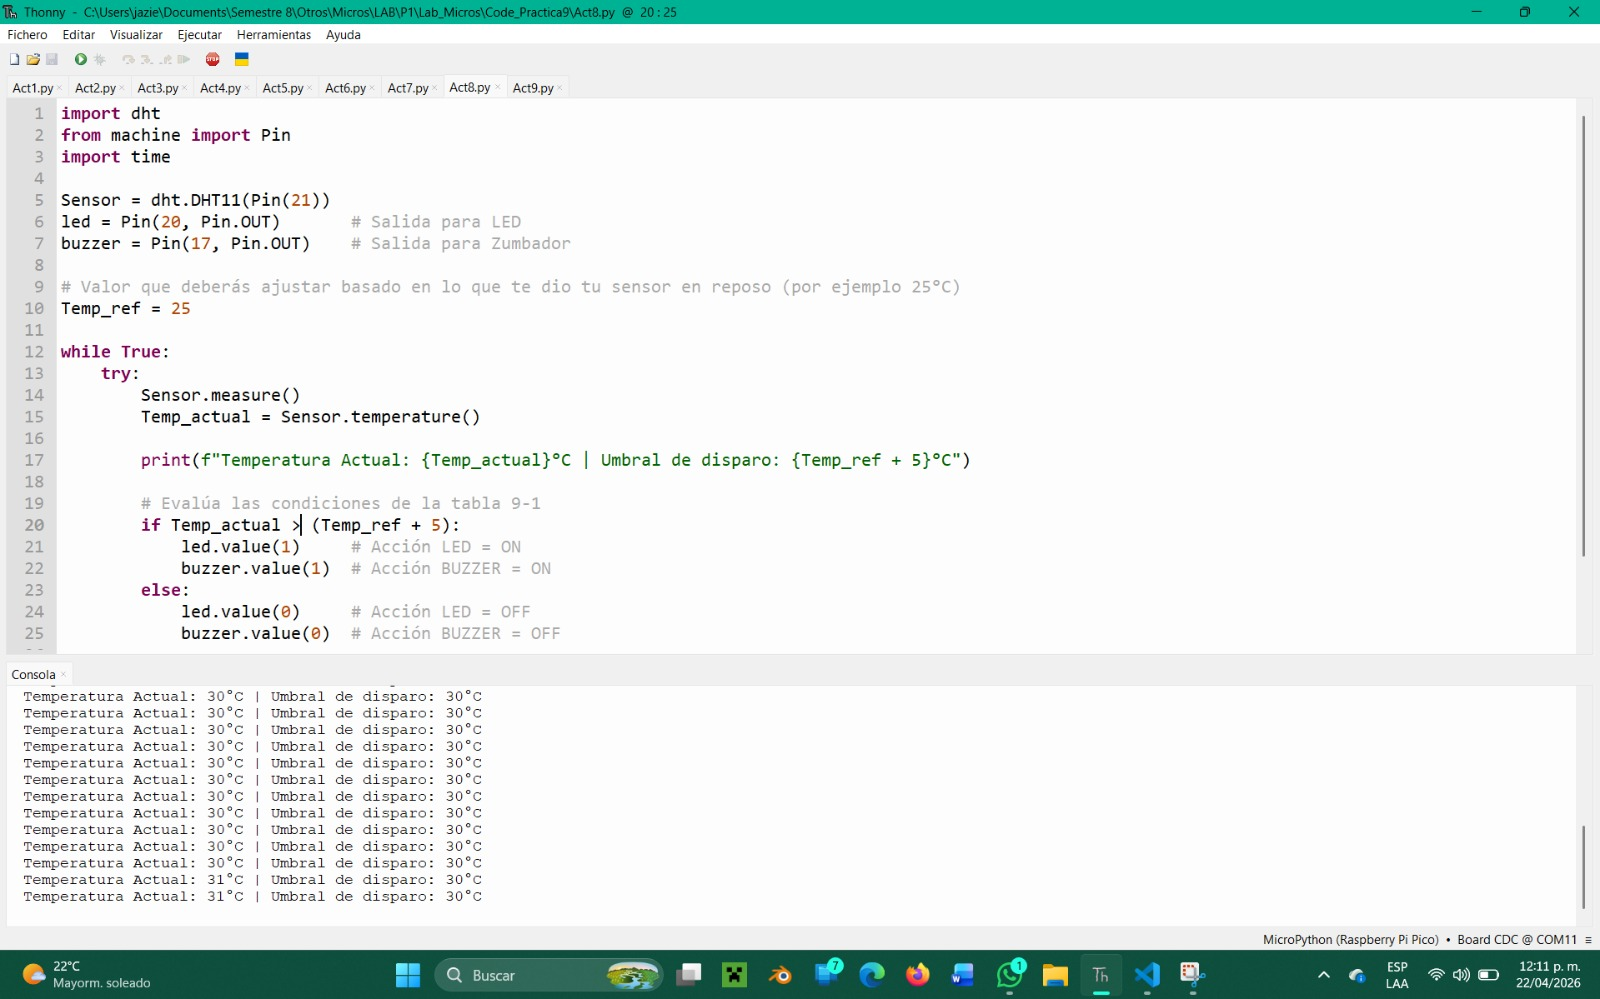
\includegraphics[width=0.75\textwidth]{img/Actividad8/Act8_2.jpg}
            \caption{Actividad 8. Medición de temperatura actual y comparación con el umbral de referencia en un segundo instante de tiempo.}
        \end{figure}
    
    \newpage

    \subsection*{Análisis de resultados}
    Al cargar el programa en la Raspberry Pi Pico, se puede observar que el programa funciona correctamente, ya que en la consola se imprime la temperatura actual y su comparación con el umbral de referencia. En el primer instante de tiempo, la temperatura actual es de 24 °C, lo que es menor que el umbral de referencia (30 °C), por lo que el LED y el zumbador permanecen apagados. En el segundo instante de tiempo, la temperatura actual es de 31 °C, lo que supera el umbral de referencia, por lo que el LED y el zumbador se activan. De forma que se puede concluir que el programa logra controlar correctamente el funcionamiento del LED y el zumbador en función de la temperatura medida por el sensor DHT11, indicando claramente cuándo la temperatura supera el umbral establecido.


    \newpage

    \section*{Actividad 9}

    \noindent Empleando los cuatro módulos usados en esta práctica, realizar un programa que controle el funcionamiento de dos semáforos con el comportamiento descrito en la \textit{actividad 10 de la practica 3}, al cabo de cada secuencia completa, mostrar el valor de la temperatura de cada uno de los sensores en un display TM1637 distinto; tal como se muestra en la tabla.

    \vspace{1cm}

    \begin{center}
    \resizebox{\textwidth}{!}{
    \begin{tikzpicture}

        % --- RASPBERRY PI PICO ---
        \picoboard

        % =========================================================
        % LADO IZQUIERDO
        % =========================================================
        
        % --- 1. DISPLAY TM1637 SUPERIOR ---
        % Título a la IZQUIERDA
        \node[text=blue!80!black, font=\sffamily\itshape\Large] at (-9.5, 0.8) {Display TM1637};
        
        % Caja principal
        \draw[thick, fill=white] (-8.5, 0.2) rectangle (-2.5, -1.2);
        
        % Cuadros internos
        \draw[thick] (-8.2, 0.0) rectangle (-7.1, -1.0);
        \draw[thick] (-6.8, 0.0) rectangle (-5.7, -1.0);
        \draw[thick] (-5.4, 0.0) rectangle (-4.3, -1.0);
        \draw[thick] (-4.0, 0.0) rectangle (-2.9, -1.0);
        
        % Cables y etiquetas lógicas (CLK Arriba, DIO Abajo)
        \draw[blue, thick] (-2.5, -0.45) -- (-0.4, -0.45); 
        \node[above, font=\sffamily\bfseries\small, inner sep=2pt] at (-1.5, -0.45) {CLK};
        
        \draw[green!70!black, thick] (-2.5, -0.90) -- (-0.4, -0.90); 
        \node[below, font=\sffamily\bfseries\small, inner sep=2pt] at (-1.5, -0.90) {DIO};
        
        % Alimentación
        \draw[red, thick] (-6.5, 0.2) -- (-6.5, 1.0); 
        \node[anchor=west, font=\sffamily\bfseries\small] at (-6.4, 0.6) {VCC};
        \node[above, font=\sffamily\footnotesize] at (-6.5, 1.0) {3.3V}; 
        \draw[red, thick] (-6.8, 1.0) -- (-6.2, 1.0);
        
        \draw[black, thick] (-4.5, -1.2) -- (-4.5, -1.8); 
        \node[anchor=west, font=\sffamily\bfseries\small] at (-4.4, -1.5) {GND};
        \draw[green!70!black, thick] (-4.9, -1.8) -- (-4.1, -1.8); 
        \draw[green!70!black, thick] (-4.7, -2.0) -- (-4.3, -2.0); 


        % --- 2. NEOPIXEL ---
        % Título a la DERECHA
        \node[text=blue!80!black, font=\sffamily\itshape\Large] at (-6.5, -1.8) {Neopixel};
        
        % Caja principal
        \draw[thick, fill=white] (-10.5, -2.4) rectangle (-2.5, -3.0);
        
        % LEDs
        \foreach \i in {0,...,7} { \draw[thick] (-9.2 + \i*0.7, -2.9) rectangle (-8.7 + \i*0.7, -2.5); }
        
        % Cables lógicos y etiquetas (Dentro de la caja)
        \draw[yellow!90!black, thick] (-2.5, -2.7) -- (-0.4, -2.7); 
        \node[anchor=east, font=\sffamily\bfseries\small] at (-2.6, -2.7) {DIN};
        
        \draw[green!60!black, thick] (-10.5, -2.7) -- (-11.5, -2.7); 
        \node[anchor=west, font=\sffamily\bfseries\small] at (-10.6, -2.7) {DOUT};
        
        % VCC muy a la izquierda para EVITAR GND de arriba
        \draw[red, thick] (-9.5, -2.4) -- (-9.5, -1.6); 
        \node[anchor=west, font=\sffamily\bfseries\small] at (-9.2, -2.0) {VCC};
        \node[above, font=\sffamily\footnotesize] at (-9.4, -1.6) {3.3V}; 
        \draw[red, thick] (-8.8, -1.6) -- (-9.8, -1.6);
        
        % GND
        \draw[black, thick] (-7.5, -3.0) -- (-7.5, -3.8); 
        \node[anchor=west, font=\sffamily\bfseries\small] at (-7.4, -3.4) {GND};
        \draw[green!70!black, thick] (-7.9, -3.8) -- (-7.1, -3.8); 
        \draw[green!70!black, thick] (-7.7, -4.0) -- (-7.3, -4.0);


        % --- 3. DISPLAY TM1637 INFERIOR ---
        % Título a la IZQUIERDA
        \node[text=blue!80!black, font=\sffamily\itshape\Large] at (-9.5, -5.0) {Display TM1637};
        
        % Caja principal
        \draw[thick, fill=white] (-8.5, -5.6) rectangle (-2.5, -7.0);
        
        % Cuadros internos
        \draw[thick] (-8.2, -5.8) rectangle (-7.1, -6.8);
        \draw[thick] (-6.8, -5.8) rectangle (-5.7, -6.8);
        \draw[thick] (-5.4, -5.8) rectangle (-4.3, -6.8);
        \draw[thick] (-4.0, -5.8) rectangle (-2.9, -6.8);
        
        % Cables y etiquetas lógicas (CLK Arriba, DIO Abajo)
        \draw[blue, thick] (-2.5, -6.30) -- (-0.4, -6.30); 
        \node[above, font=\sffamily\bfseries\small, inner sep=2pt] at (-1.5, -6.30) {CLK};
        
        \draw[green!70!black, thick] (-2.5, -6.75) -- (-0.4, -6.75); 
        \node[below, font=\sffamily\bfseries\small, inner sep=2pt] at (-1.5, -6.75) {DIO};
        
        % Alimentación
        \draw[red, thick] (-6.5, -5.6) -- (-6.5, -4.8); 
        \node[anchor=west, font=\sffamily\bfseries\small] at (-6.4, -5.2) {VCC};
        \node[above, font=\sffamily\footnotesize] at (-6.5, -4.8) {3.3V}; 
        \draw[red, thick] (-6.8, -4.8) -- (-6.2, -4.8);
        
        \draw[black, thick] (-4.5, -7.0) -- (-4.5, -7.8); 
        \node[anchor=west, font=\sffamily\bfseries\small] at (-4.4, -7.4) {GND};
        \draw[green!70!black, thick] (-4.9, -7.8) -- (-4.1, -7.8); 
        \draw[green!70!black, thick] (-4.7, -8.0) -- (-4.3, -8.0);


        % =========================================================
        % LADO DERECHO 
        % =========================================================

        % --- 4. SENSOR DTH11 ---
        % Título a la DERECHA para despejar el VCC
        \node[align=center, text=blue!80!black, font=\sffamily\bfseries\small] at (9.5, -3.0) {Sensor de\\[0.1cm]Temperatura\\[0.1cm]y Humedad\\[0.1cm]DTH11};
        
        % Caja
        \draw[thick, fill=white] (6.5, -4.5) rectangle (8.5, -7.5);
        
        % Cable S
        \draw[blue!80!cyan, thick] (4.4, -6.30) -- (6.5, -6.30); 
        \node[anchor=west, font=\sffamily\bfseries\Large] at (6.6, -6.30) {S};
        
        % Alimentación
        \draw[red, thick] (7.5, -4.5) -- (7.5, -3.8); 
        \node[anchor=west, font=\sffamily\bfseries\small] at (7.6, -4.15) {VCC};
        \node[above, font=\sffamily\footnotesize] at (7.5, -3.8) {3.3V}; 
        \draw[red, thick] (7.2, -3.8) -- (7.8, -3.8);
        
        \draw[black, thick] (7.5, -7.5) -- (7.5, -8.2); 
        \node[anchor=west, font=\sffamily\bfseries\small] at (7.6, -7.85) {GND};
        \draw[green!70!black, thick] (7.1, -8.2) -- (7.9, -8.2); 
        \draw[green!70!black, thick] (7.3, -8.35) -- (7.7, -8.35);


        % --- 5. SENSOR DS18B20 ---
        % Módulo movido MAS ABAJO (Caja ajustada a Y=-10.0 a -12.5)
        \node[font=\sffamily\scriptsize] at (9.0, -9.6) {Sensor de Temperatura DS18B20};
        \draw[line width=1.5pt, fill=white] (7.0, -10.0) rectangle (11.0, -12.5);
        \node[font=\sffamily\Large] at (9.0, -11.25) {DS18B20};
        
        % Etiquetas
        \node[anchor=west, font=\sffamily\small] at (7.1, -10.2) {VDD};
        \node[anchor=west, font=\sffamily\small] at (7.1, -10.5) {DQ};
        \node[anchor=west, font=\sffamily\small] at (7.1, -12.0) {GND};
        
        % Cuadros verdes
        \draw[green!80!black, thick, fill=green!20, opacity=0.8] (6.4, -10.35) rectangle (6.7, -10.05);
        \draw[green!80!black, thick, fill=green!20, opacity=0.8] (6.4, -10.65) rectangle (6.7, -10.35);
        \draw[green!80!black, thick, fill=green!20, opacity=0.8] (6.4, -12.15) rectangle (6.7, -11.85);

        % Cable DQ bajando ortogonalmente para conectar correctamente sin cruzar
        \draw[orange!90!black, thick] (4.4, -9.0) -- (5.0, -9.0) -- (5.0, -10.5) -- (7.0, -10.5); 
        
        % VDD
        \draw[line width=1.5pt] (7.0, -10.2) -- (6.0, -10.2); 
        \draw[thick] (6.0, -10.2) -- (6.0, -8.6); 
        \node[above, font=\sffamily\bfseries\small] at (6.0, -8.6) {3.3V}; 
        \draw[thick] (5.7, -8.6) -- (6.3, -8.6);
        
        % GND
        \draw[line width=1.5pt] (7.0, -12.0) -- (6.0, -12.0); 
        \draw[thick] (6.0, -12.0) -- (6.0, -12.8); 
        \draw[green!70!black, thick] (5.6, -12.8) -- (6.4, -12.8); 
        \draw[green!70!black, thick] (5.8, -12.95) -- (6.2, -12.95);

    \end{tikzpicture}
    } 
    \end{center}

    \begin{center}
        % Configuración de las tablas
        \sffamily % Fuente Sans Serif para todo el bloque
        \setlength{\arrayrulewidth}{0.5pt}
        \arrayrulecolor{gray!50} % Color sutil para los bordes de las tablas
        \renewcommand{\arraystretch}{1.3} % Espaciado vertical interno

        % ==========================================
        % PRIMERA FILA DE TABLAS
        % ==========================================
        \begin{minipage}[t]{0.32\textwidth}
            \centering
            \textbf{\textit{Semáforo}}\\[0.3cm]
            \setlength{\tabcolsep}{6pt}
            
            % Semáforo 1 escalado
            \scalebox{0.8}{
            \begin{tabular}{|c|c|c|}
                \hline
                \cellcolor{SemGreen}V1 & \cellcolor{SemYellow}A1 & \cellcolor{SemRed}\textcolor{white}{R1} \\
                \hline
            \end{tabular}
            }
            \quad % Espacio entre semáforos
            % Semáforo 2 escalado
            \scalebox{0.8}{
            \begin{tabular}{|c|c|c|}
                \hline
                \cellcolor{SemGreen}V2 & \cellcolor{SemYellow}A2 & \cellcolor{SemRed}\textcolor{white}{R2} \\
                \hline
            \end{tabular}
            }
        \end{minipage}
        \hfill
        \begin{minipage}[t]{0.32\textwidth}
            \centering
            \textbf{\textit{Display TM1637}}\\[0.3cm]
            \scalebox{0.8}{
            \begin{tabular}{|>{\centering\arraybackslash}p{2.2cm}|>{\centering\arraybackslash}p{2.2cm}|}
                \hline
                \rowcolor{TabOrangeHead} \textcolor{white}{\textbf{\textit{CLK}}} & \textcolor{white}{\textbf{\textit{DIO}}} \\
                \hline
                \rowcolor{TabOrangeBody} \textbf{\textit{GPIO0}} & \textbf{\textit{GPIO1}} \\
                \hline
            \end{tabular}
            }
        \end{minipage}
        \hfill
        \begin{minipage}[t]{0.32\textwidth}
            \centering
            \textbf{\textit{Display TM1637}}\\[0.3cm]
            \scalebox{0.8}{
            \begin{tabular}{|>{\centering\arraybackslash}p{2.2cm}|>{\centering\arraybackslash}p{2.2cm}|}
                \hline
                \rowcolor{TabGreyHead} \textcolor{white}{\textbf{\textit{CLK}}} & \textcolor{white}{\textbf{\textit{DIO}}} \\
                \hline
                \rowcolor{TabGreyBody} \textbf{\textit{GPIO10}} & \textbf{\textit{GPIO11}} \\
                \hline
            \end{tabular}
            }
        \end{minipage}

        \vspace{0.8cm} % Espacio entre la primera y segunda fila

        % ==========================================
        % SEGUNDA FILA DE TABLAS
        % ==========================================
        \begin{minipage}[t]{0.36\textwidth}
            \centering
            \scalebox{0.8}{
            \begin{tabular}{|>{\centering\arraybackslash}p{6cm}|}
                \hline
                \rowcolor{TabBlueHead} \textcolor{white}{\textit{Barra leds Neopixel}} \\
                \hline
                \rowcolor{TabBlueBody} \textbf{GPIO4} \\
                \hline
            \end{tabular}
            }
        \end{minipage}
        \hfill
        \begin{minipage}[t]{0.30\textwidth}
            \centering
            \scalebox{0.8}{
            \begin{tabular}{|>{\centering\arraybackslash}p{4.5cm}|}
                \hline
                \rowcolor{TabOrangeHead} \textcolor{white}{\textit{Temperatura DS18B20}} \\
                \hline
                \rowcolor{TabOrangeBody} \textbf{GPIO16} \\
                \hline
            \end{tabular}
            }
        \end{minipage}
        \hfill
        \begin{minipage}[t]{0.30\textwidth}
            \centering
            \scalebox{0.8}{
            \begin{tabular}{|>{\centering\arraybackslash}p{4.5cm}|}
                \hline
                \rowcolor{TabGreyHead} \textcolor{white}{\textit{Temperatura DHT11}} \\
                \hline
                \rowcolor{TabGreyBody} \textbf{GPIO21} \\
                \hline
            \end{tabular}
            }
        \end{minipage}

        \vspace{0.8cm}
        
        % ==========================================
        % PIE DE FIGURA
        % ==========================================
        Figura 9-16. Especificaciones y esquemático; actividad 9
        
    \end{center}


    \section*{Propuesta de solución}
    Para integrar múltiples periféricos, se propone un sistema secuencial dividido en dos fases. La Fase A controla una tira de LEDs direccionables (Neopixel) para emular un cruce de semáforos, manipulando los canales de color (RGB) de píxeles específicos con tiempos de bloqueo asignados. 
    
    La Fase B realiza un monitoreo térmico durante una ventana de 10 segundos utilizando el DS18B20 y el DHT11. Para consolidar la salida visual y optimizar el hardware, la solución centraliza las lecturas en un único display TM1637. El programa utiliza una variable de estado (\texttt{modo\_sensor}) para determinar cuál sensor se procesará en el bucle actual. Para alternar entre ellos a petición del usuario, se configura un botón físico en el GPIO 13 que dispara una interrupción de hardware, invirtiendo la variable de estado de forma instantánea sin importar en qué parte del ciclo de visualización se encuentre el procesador.

    \begin{center}
        \scalebox{0.78}{
        \begin{tikzpicture}[node distance=1.05cm, every node/.style={font=\scriptsize}]
            \node (start9) [startstop, text width=3.0cm] {Inicio};
            \node (init9) [process, below=of start9, text width=8.8cm] {Inicializar Neopixel, TM1637, DS18B20 y DHT11. Configurar IRQ del boton (GPIO13) para alternar \texttt{modo\_sensor}.};
            \node (fasea9) [process, below=of init9, text width=8.8cm] {Fase A: ejecutar la secuencia de semaforos (verdes, amarillos, rojos e intermitencias).};
            \node (timer9) [process, below=of fasea9, text width=7.4cm] {Fase B: \texttt{inicio\_fase = time.time()}.};
            \node (tcheck9) [decision, below=of timer9, text width=3.3cm, aspect=2.1] {\texttt{time.time()-inicio\_fase < 10}?};
            \node (modo9) [decision, below=of tcheck9, text width=3.3cm, aspect=2.1] {\texttt{modo\_sensor == 0}?};

            \node (ds9) [process, below left=1.2cm and 2.3cm of modo9, text width=4.6cm] {Ruta DS18B20:\newline \texttt{scan()}, \texttt{convert\_temp()}, esperar 750 ms, leer y mostrar \texttt{"DS"} + valor.};
            \node (dht9) [process, below right=1.2cm and 2.3cm of modo9, text width=4.6cm] {Ruta DHT11:\newline \texttt{measure()}, leer temperatura y mostrar \texttt{"DH"} + valor.};
            \node (exc9) [decision, below=of modo9, yshift=-2.3cm, text width=3.0cm, aspect=2.1] {\texttt{Excepcion\newline de lectura?}};
            \node (err9) [process, right=2.3cm of exc9, text width=3.6cm] {Mostrar error:\newline \texttt{tm.show("ERR ")}.};
            \node (wait9) [process, below=of exc9, text width=4.0cm] {Esperar 1 s.};
            \node (clear9) [process, right=2.9cm of tcheck9, text width=4.2cm] {Limpiar display:\newline \texttt{tm.write([0,0,0,0])}.};

            \draw [arrow] (start9) -- (init9);
            \draw [arrow] (init9) -- (fasea9);
            \draw [arrow] (fasea9) -- (timer9);
            \draw [arrow] (timer9) -- (tcheck9);
            \draw [arrow] (tcheck9) -- node[right] {Si} (modo9);
            \draw [arrow] (modo9) -- node[above left, font=\scriptsize] {Si} (ds9);
            \draw [arrow] (modo9) -- node[above right, font=\scriptsize] {No} (dht9);

            % --- CORRECCIONES A PARTIR DE AQUÍ ---
            
            % 1. Las ramas de los sensores se unen limpiamente y entran por el NORTE del rombo de excepción
            \draw (ds9.south) |- ([yshift=0.6cm]exc9.north);
            \draw (dht9.south) |- ([yshift=0.6cm]exc9.north);
            \draw [arrow] ([yshift=0.6cm]exc9.north) -- (exc9.north);

            % 2. El bloque de error (err9) recibe la respuesta "Si" por su izquierda y baja directo al "esperar 1s"
            \draw [arrow] (exc9.east) -- node[above, font=\scriptsize] {Si} (err9.west);
            \draw [arrow] (err9.south) |- (wait9.east);

            % 3. Si no hay error ("No"), baja recto sin cruces
            \draw [arrow] (exc9.south) -- node[left, font=\scriptsize] {No} (wait9.north);

            % 4. La flecha de retorno general sale por la izquierda y rodea el bloque ds9 para no pisarlo
            \draw [arrow] (wait9.west) -| ([xshift=-0.8cm]ds9.west) |- (tcheck9.west);

            % --- FIN DE CORRECCIONES ---

            \draw [arrow] (tcheck9.east) -- node[above, font=\scriptsize] {No} (clear9.west);
            \draw [arrow] (clear9.north) |- (fasea9.east);
        \end{tikzpicture}
        }
    \end{center}

    El flujo de datos integra dos ciclos anidados: primero la fase de semaforos, donde se escriben secuencias RGB sobre Neopixel, y despues la fase de monitoreo de 10 segundos, donde el dato termico se enruta segun \texttt{modo\_sensor}. Si el modo es 0, el dato proviene del DS18B20 (escaneo, conversion y lectura); en modo 1, proviene del DHT11 (muestreo y lectura directa). En ambos casos el valor se transforma a entero para desplegarse en TM1637 con una etiqueta de contexto (DS o DH). Si ocurre una excepcion, el flujo desvía la salida hacia \texttt{ERR}. Al finalizar la ventana temporal, se limpia el display y se reinicia la secuencia completa; en paralelo, la interrupcion del boton puede cambiar la ruta de datos en cualquier instante.

    \section*{Desarrollo}

    \lstinputlisting[language={[LAB]Python}, caption=Código de la Actividad 9, basicstyle=\ttfamily\scriptsize]{Code/Act9.py}

    \begin{figure}[H]
        \centering
        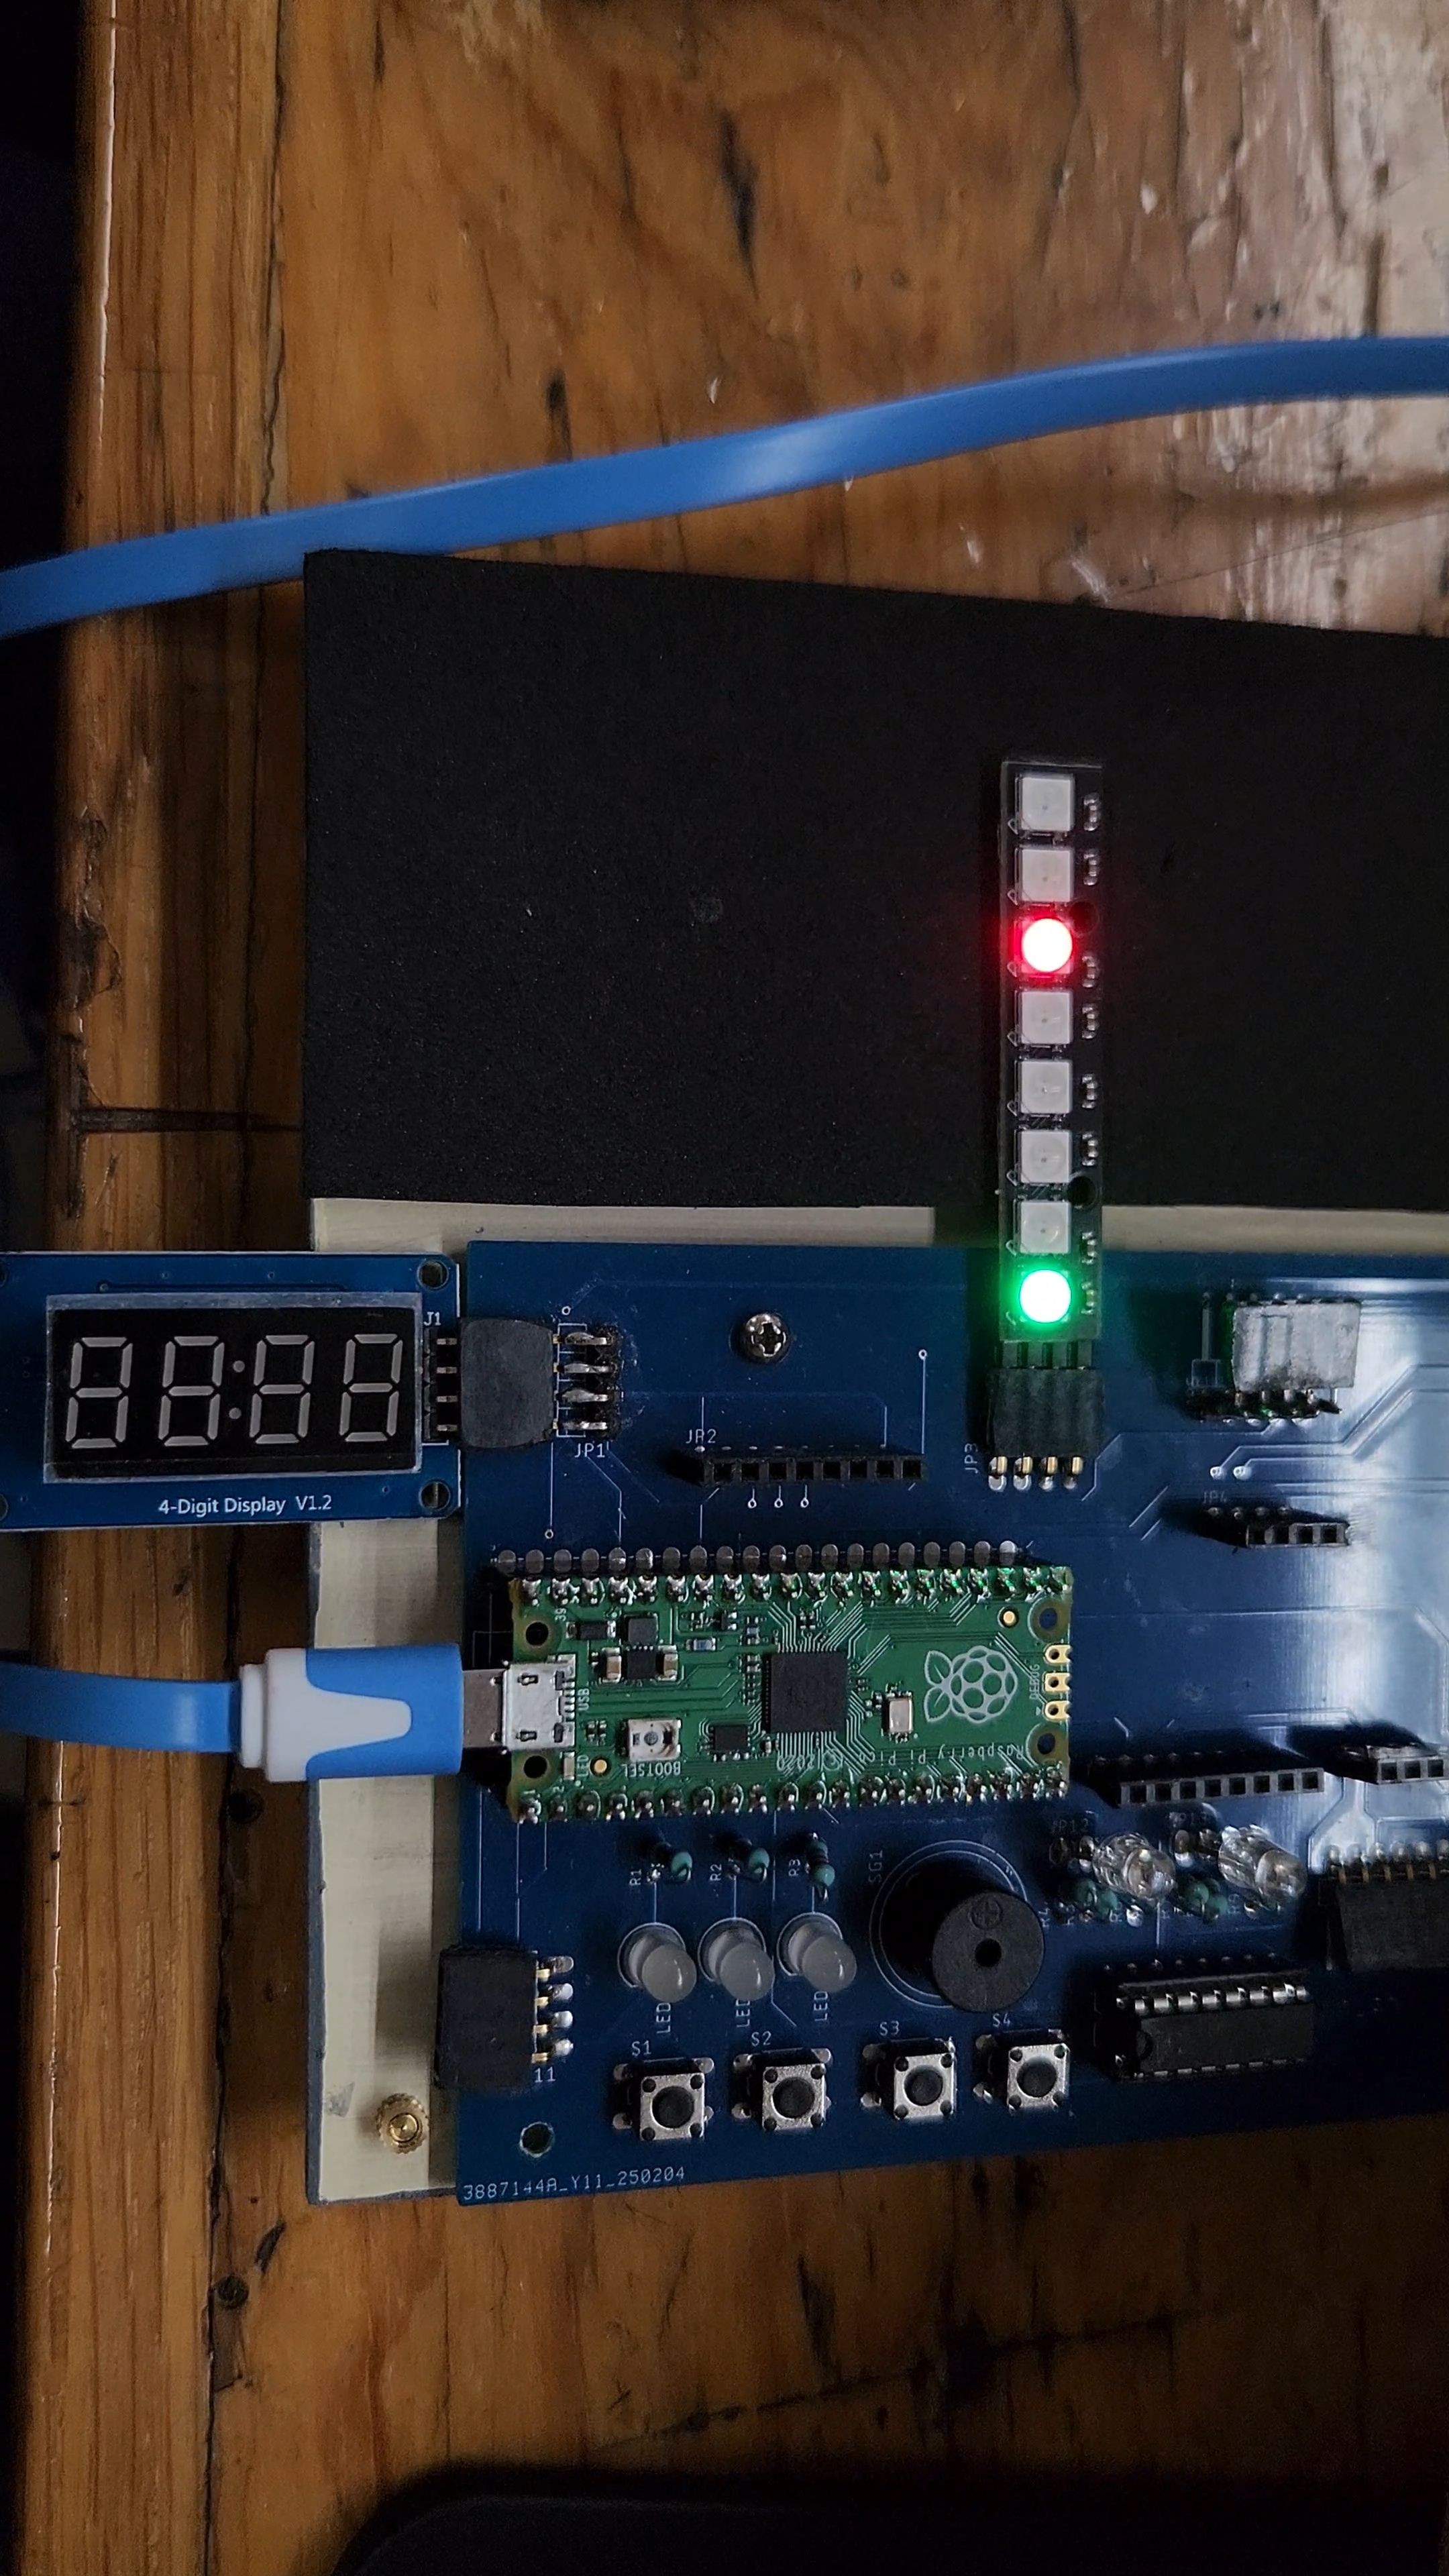
\includegraphics[width=0.5\textwidth, angle=90]{img/Actividad9/Act9_3.jpg}
        \caption{Inicio de la Fase A (Secuencia de tráfico). El microcontrolador comanda la barra Neopixel estableciendo el píxel 0 en verde y el píxel 5 en rojo mediante ráfagas de 800 kHz. Esto emula el estado inicial del cruce (V1 y R2 activos).}
    \end{figure}

    \begin{figure}[H]
        \centering
        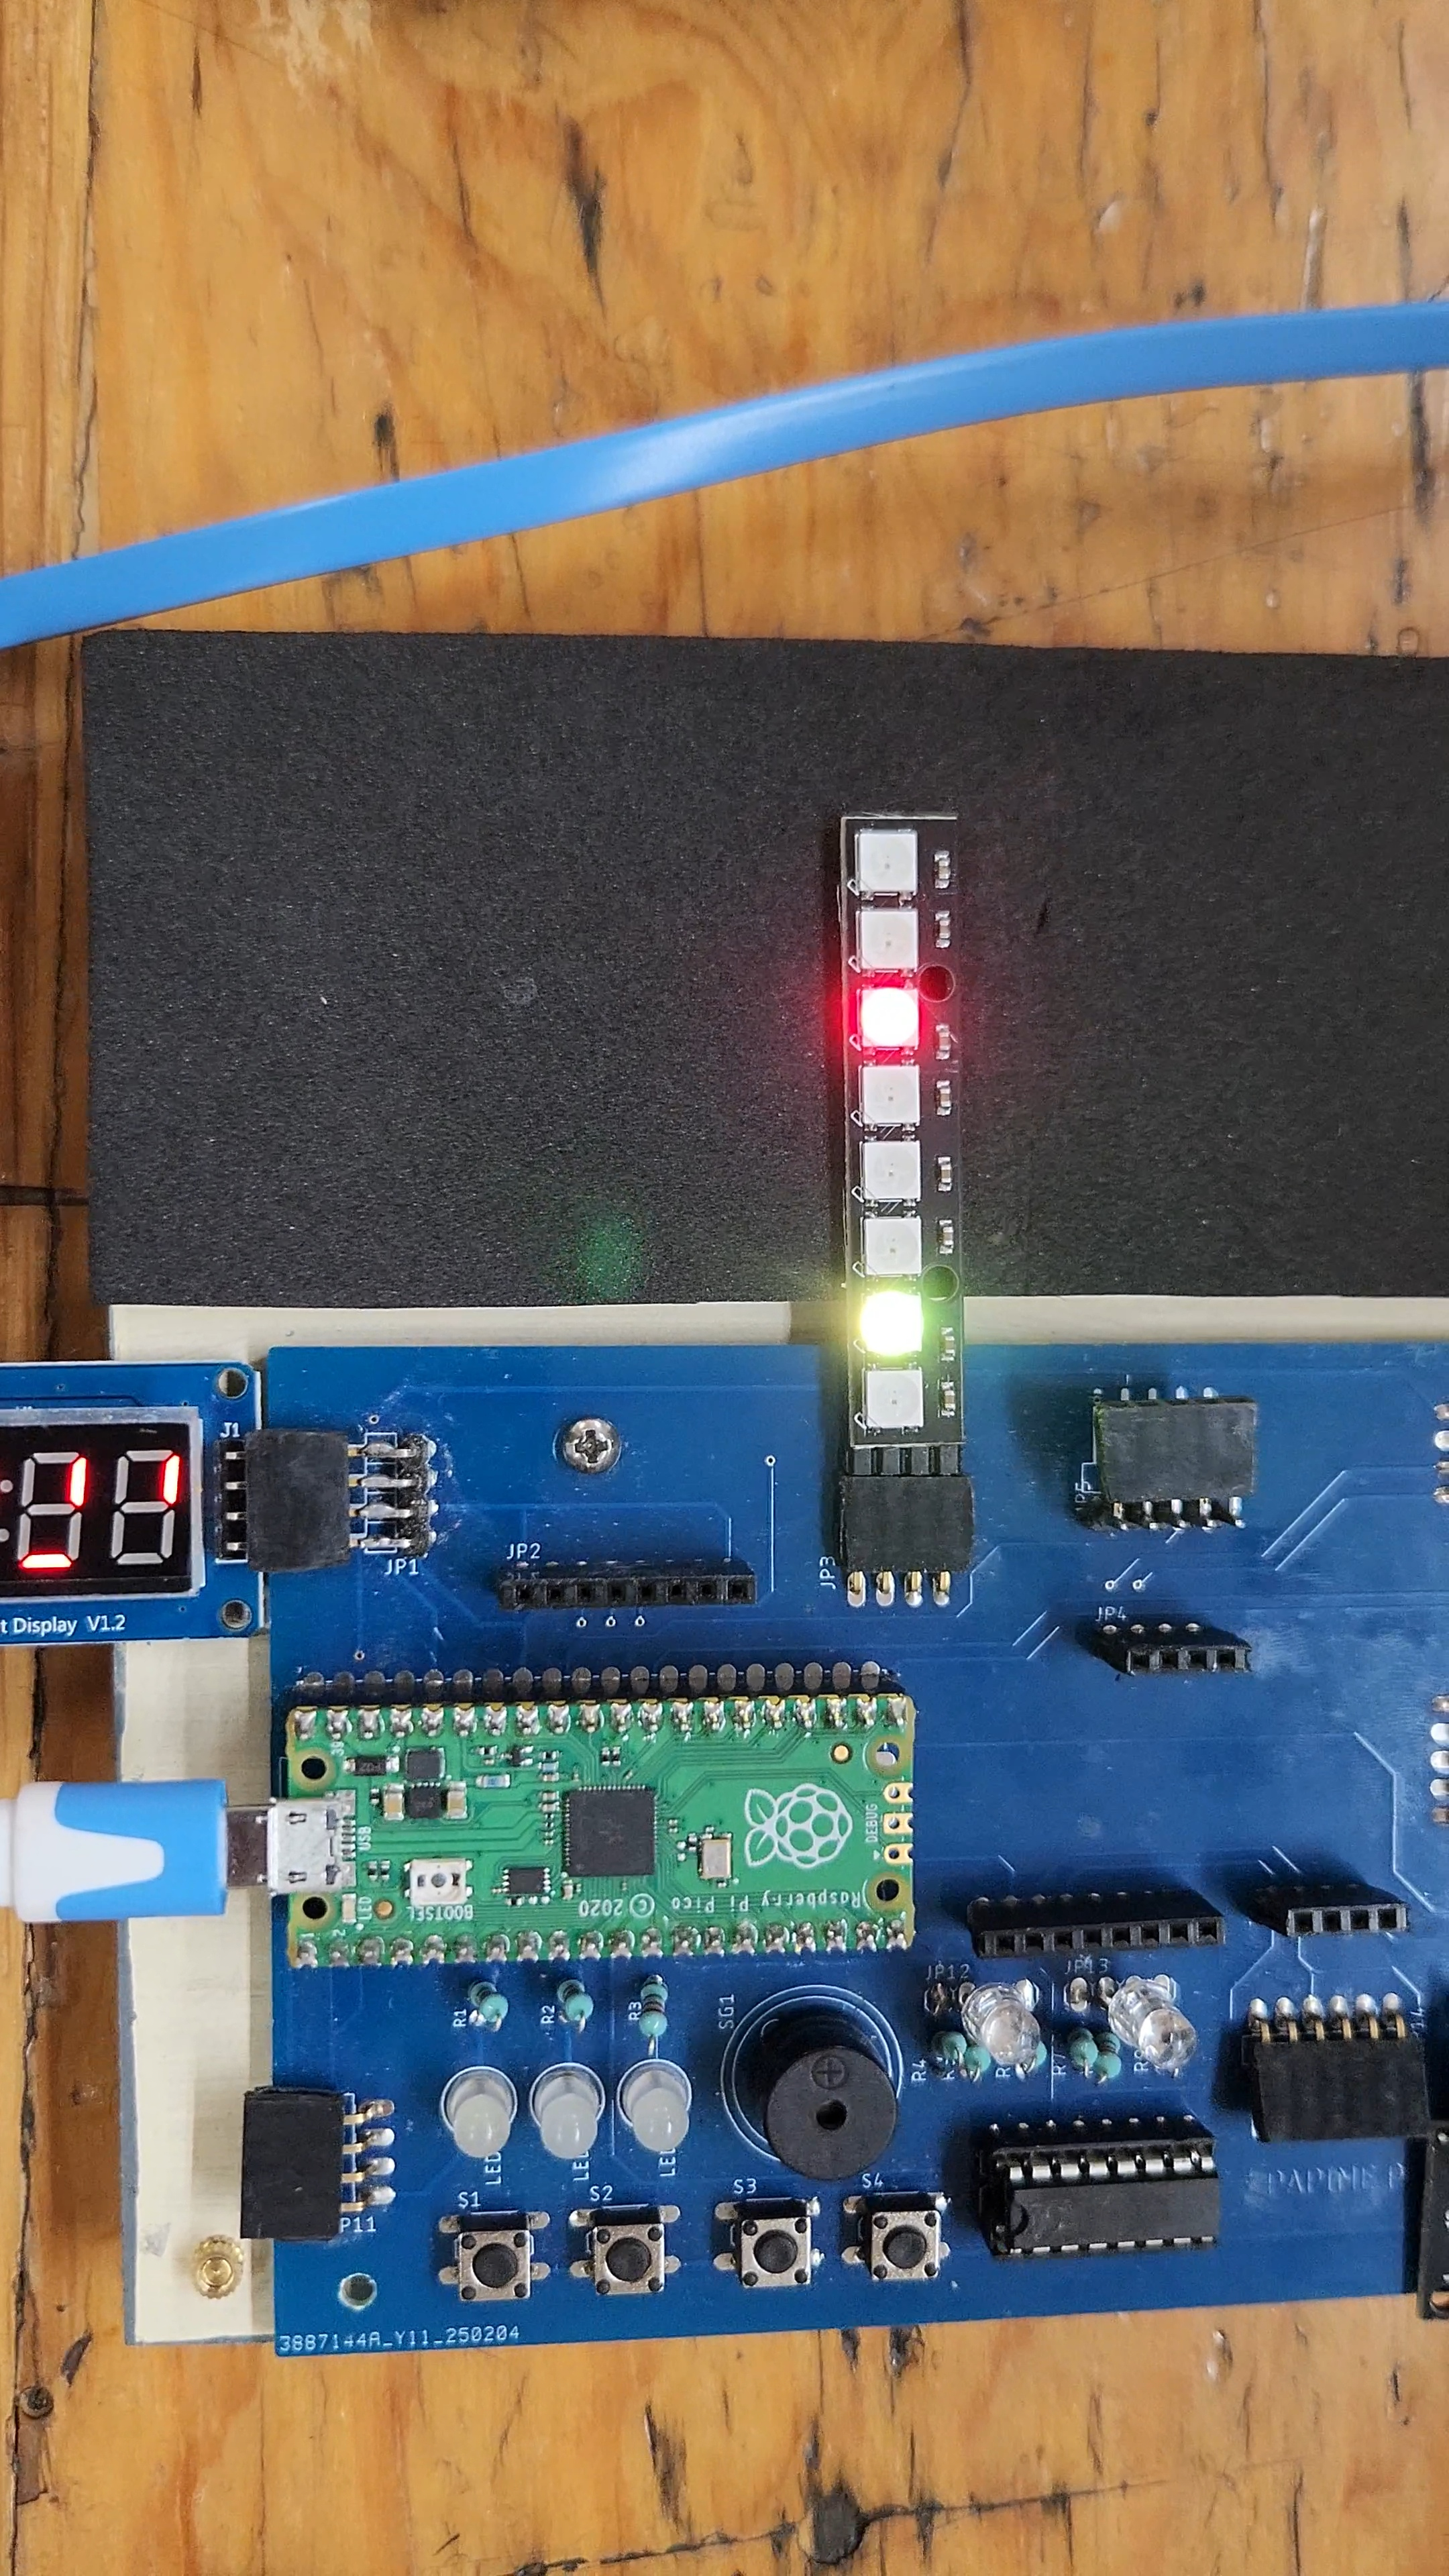
\includegraphics[width=0.4\textwidth, angle=90]{img/Actividad9/Act9_12.jpg}
        \caption{Transición de precaución en el primer semáforo. El algoritmo apaga el LED verde y satura el píxel 1 con los canales rojo y verde al 100\% para generar el color amarillo (A1), manteniendo el segundo semáforo bloqueado en rojo (R2).}
    \end{figure}

    \begin{figure}[H]
        \centering
        
\includegraphics[width=0.4\textwidth, angle=90]{img/Actividad9/Act9_1.jpg}
        \caption{Inversión del flujo vehicular. El primer semáforo pasa a estado de detención iluminando el píxel 2 en rojo (R1), mientras que se habilita el paso en el segundo carril encendiendo el píxel 3 en color verde (V2).}
    \end{figure}

    \begin{figure}[H]
        \centering
        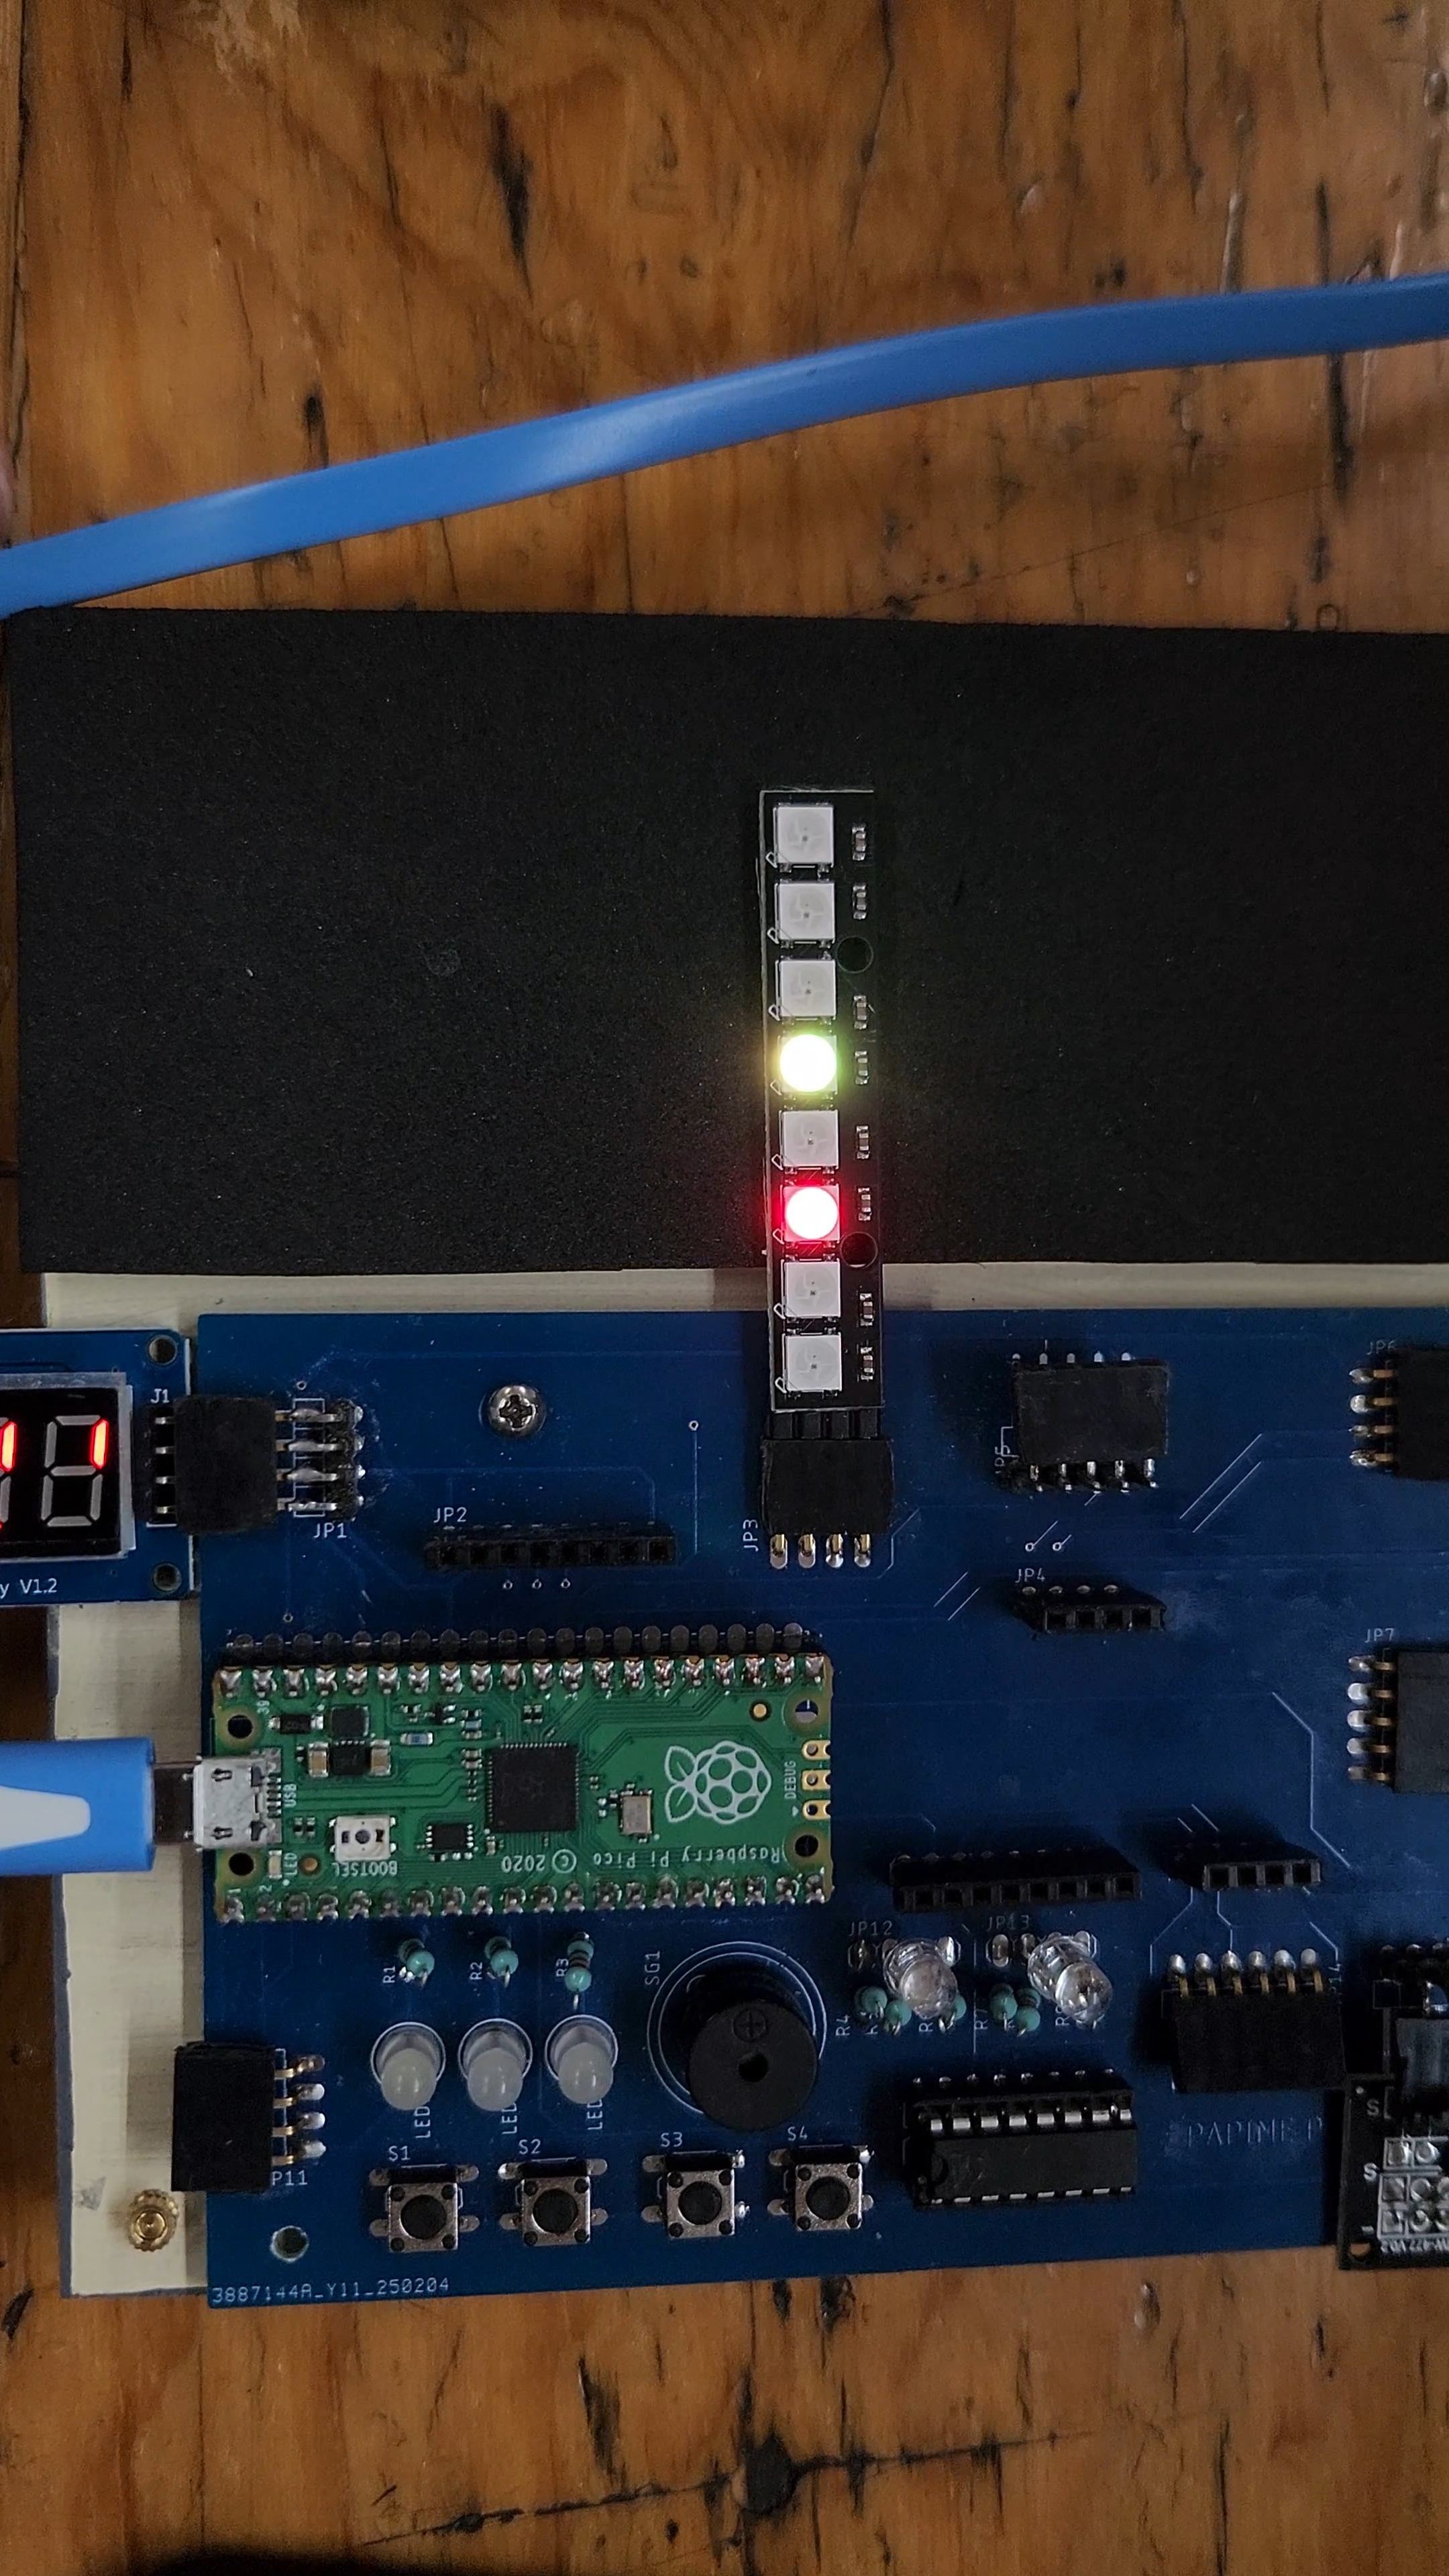
\includegraphics[width=0.4\textwidth, angle=90]{img/Actividad9/Act9_6.jpg}
        \caption{Finalización del ciclo de tráfico. El píxel 4 cambia a amarillo (A2) indicando precaución en el segundo semáforo, preparándose para apagar la barra completa y liberar los recursos del procesador para la etapa de sensado.}
    \end{figure}

    \begin{figure}[H]
        \centering
        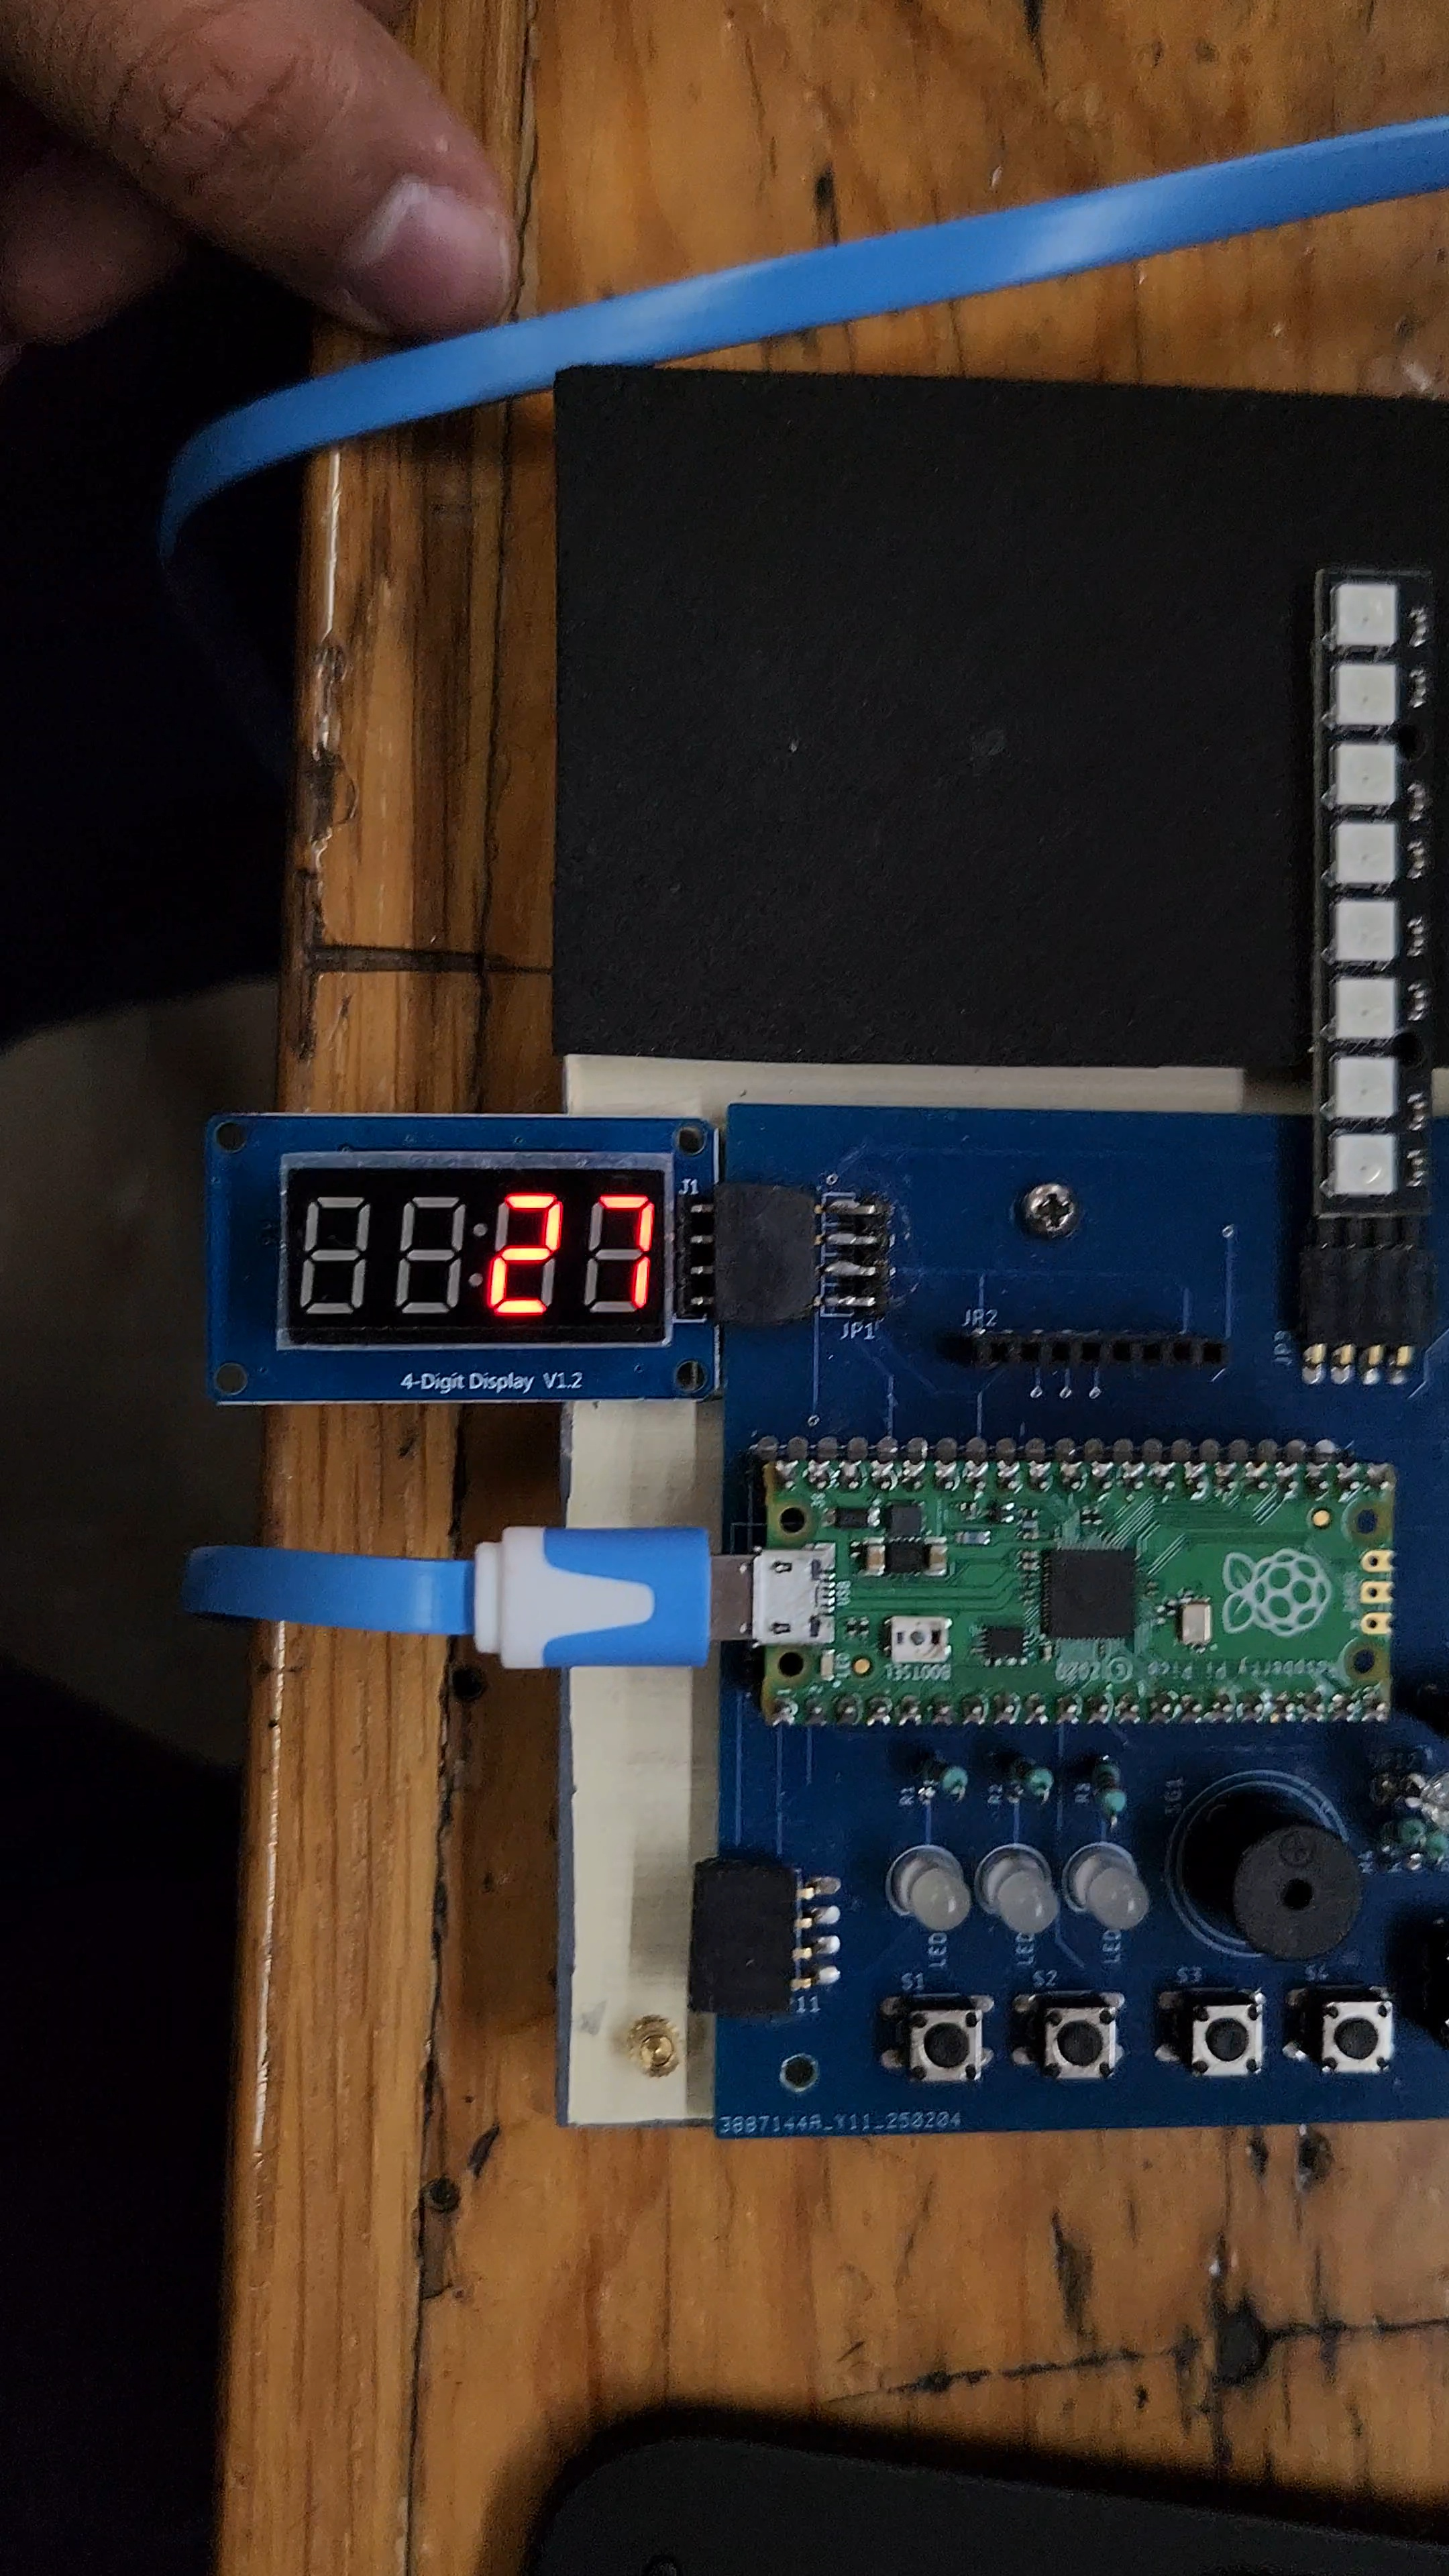
\includegraphics[width=0.4\textwidth, angle=90]{img/Actividad9/Act9_8.jpg}
        \caption{Inicio de la Fase B (Monitoreo térmico). La barra Neopixel se apaga. El programa entra al bloque del sensor DS18B20 (\texttt{modo\_sensor == 0}) e imprime el prefijo "dS" en el display TM1637 como identificador visual antes de procesar el dato numérico.}
    \end{figure}

    \begin{figure}[H]
        \centering
        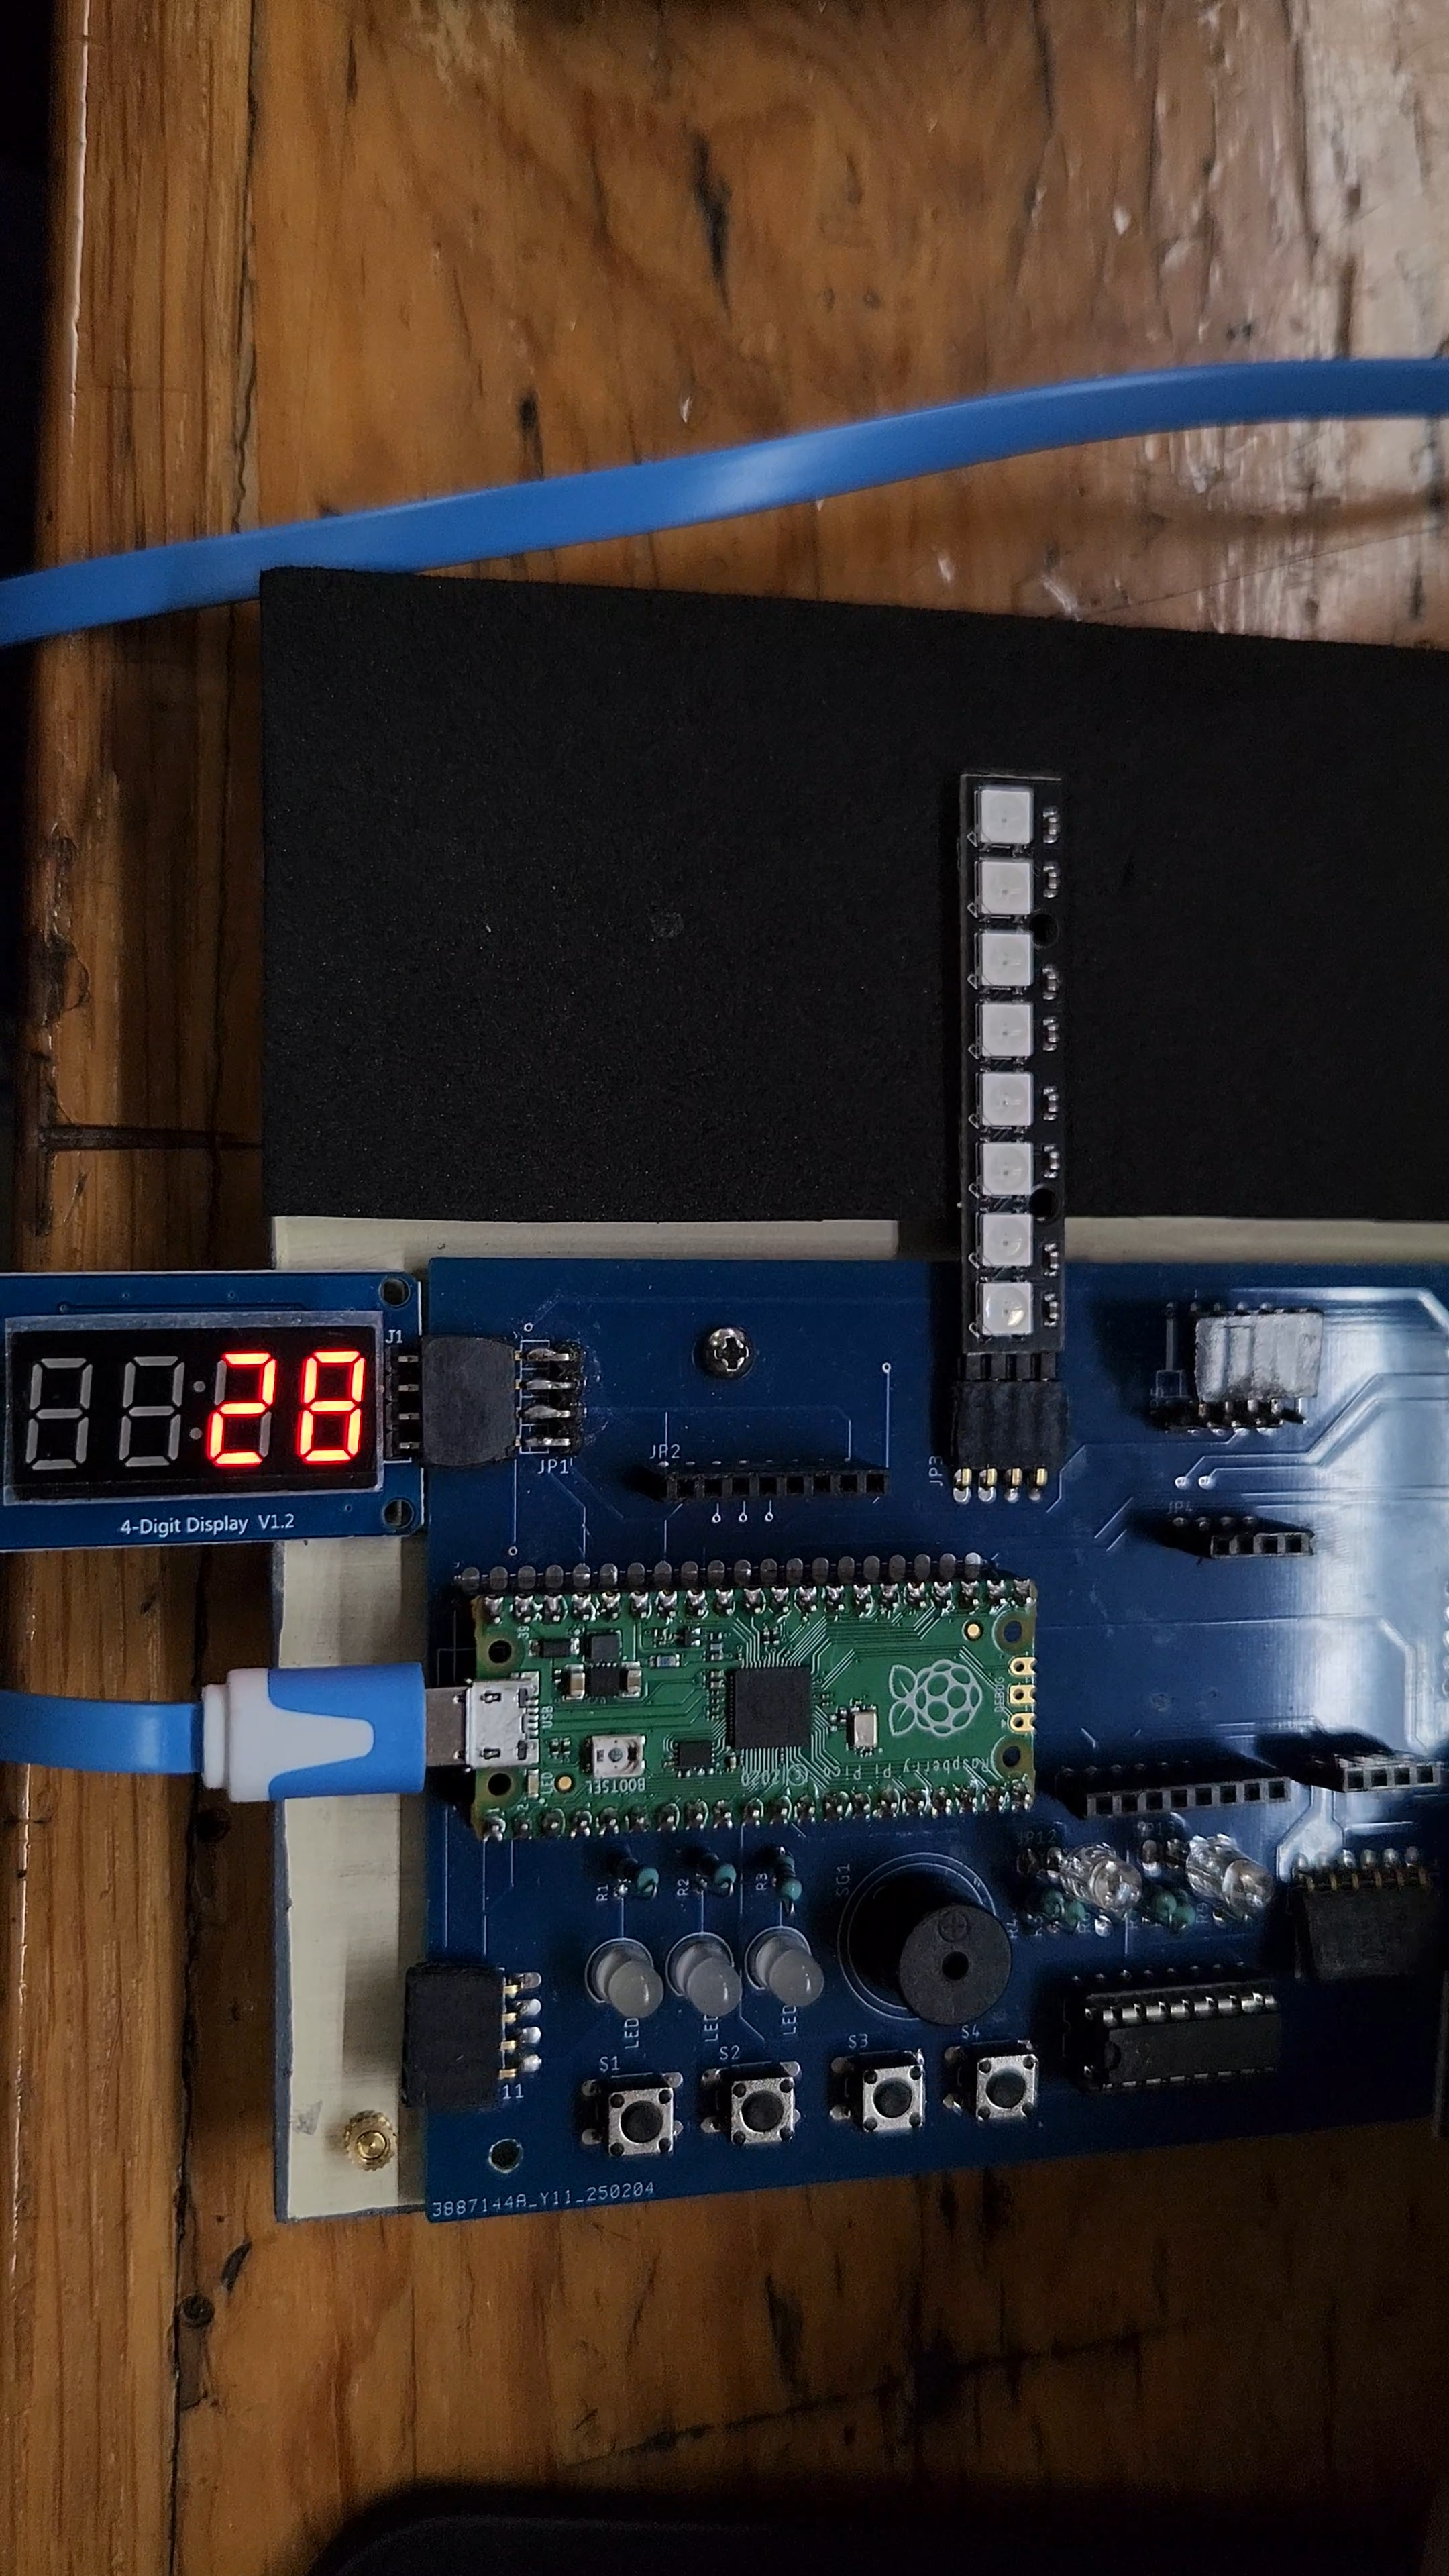
\includegraphics[width=0.4\textwidth, angle=90]{img/Actividad9/Act9_2.jpg}
        \caption{Lectura del protocolo \textit{1-Wire}. Tras cumplir el tiempo de conversión de 750 ms, el DS18B20 arroja la temperatura ambiental. El microcontrolador formatea el valor entero y actualiza el display para mostrar "dS 28" (28 °C).}
    \end{figure}

    \begin{figure}[H]
        \centering
        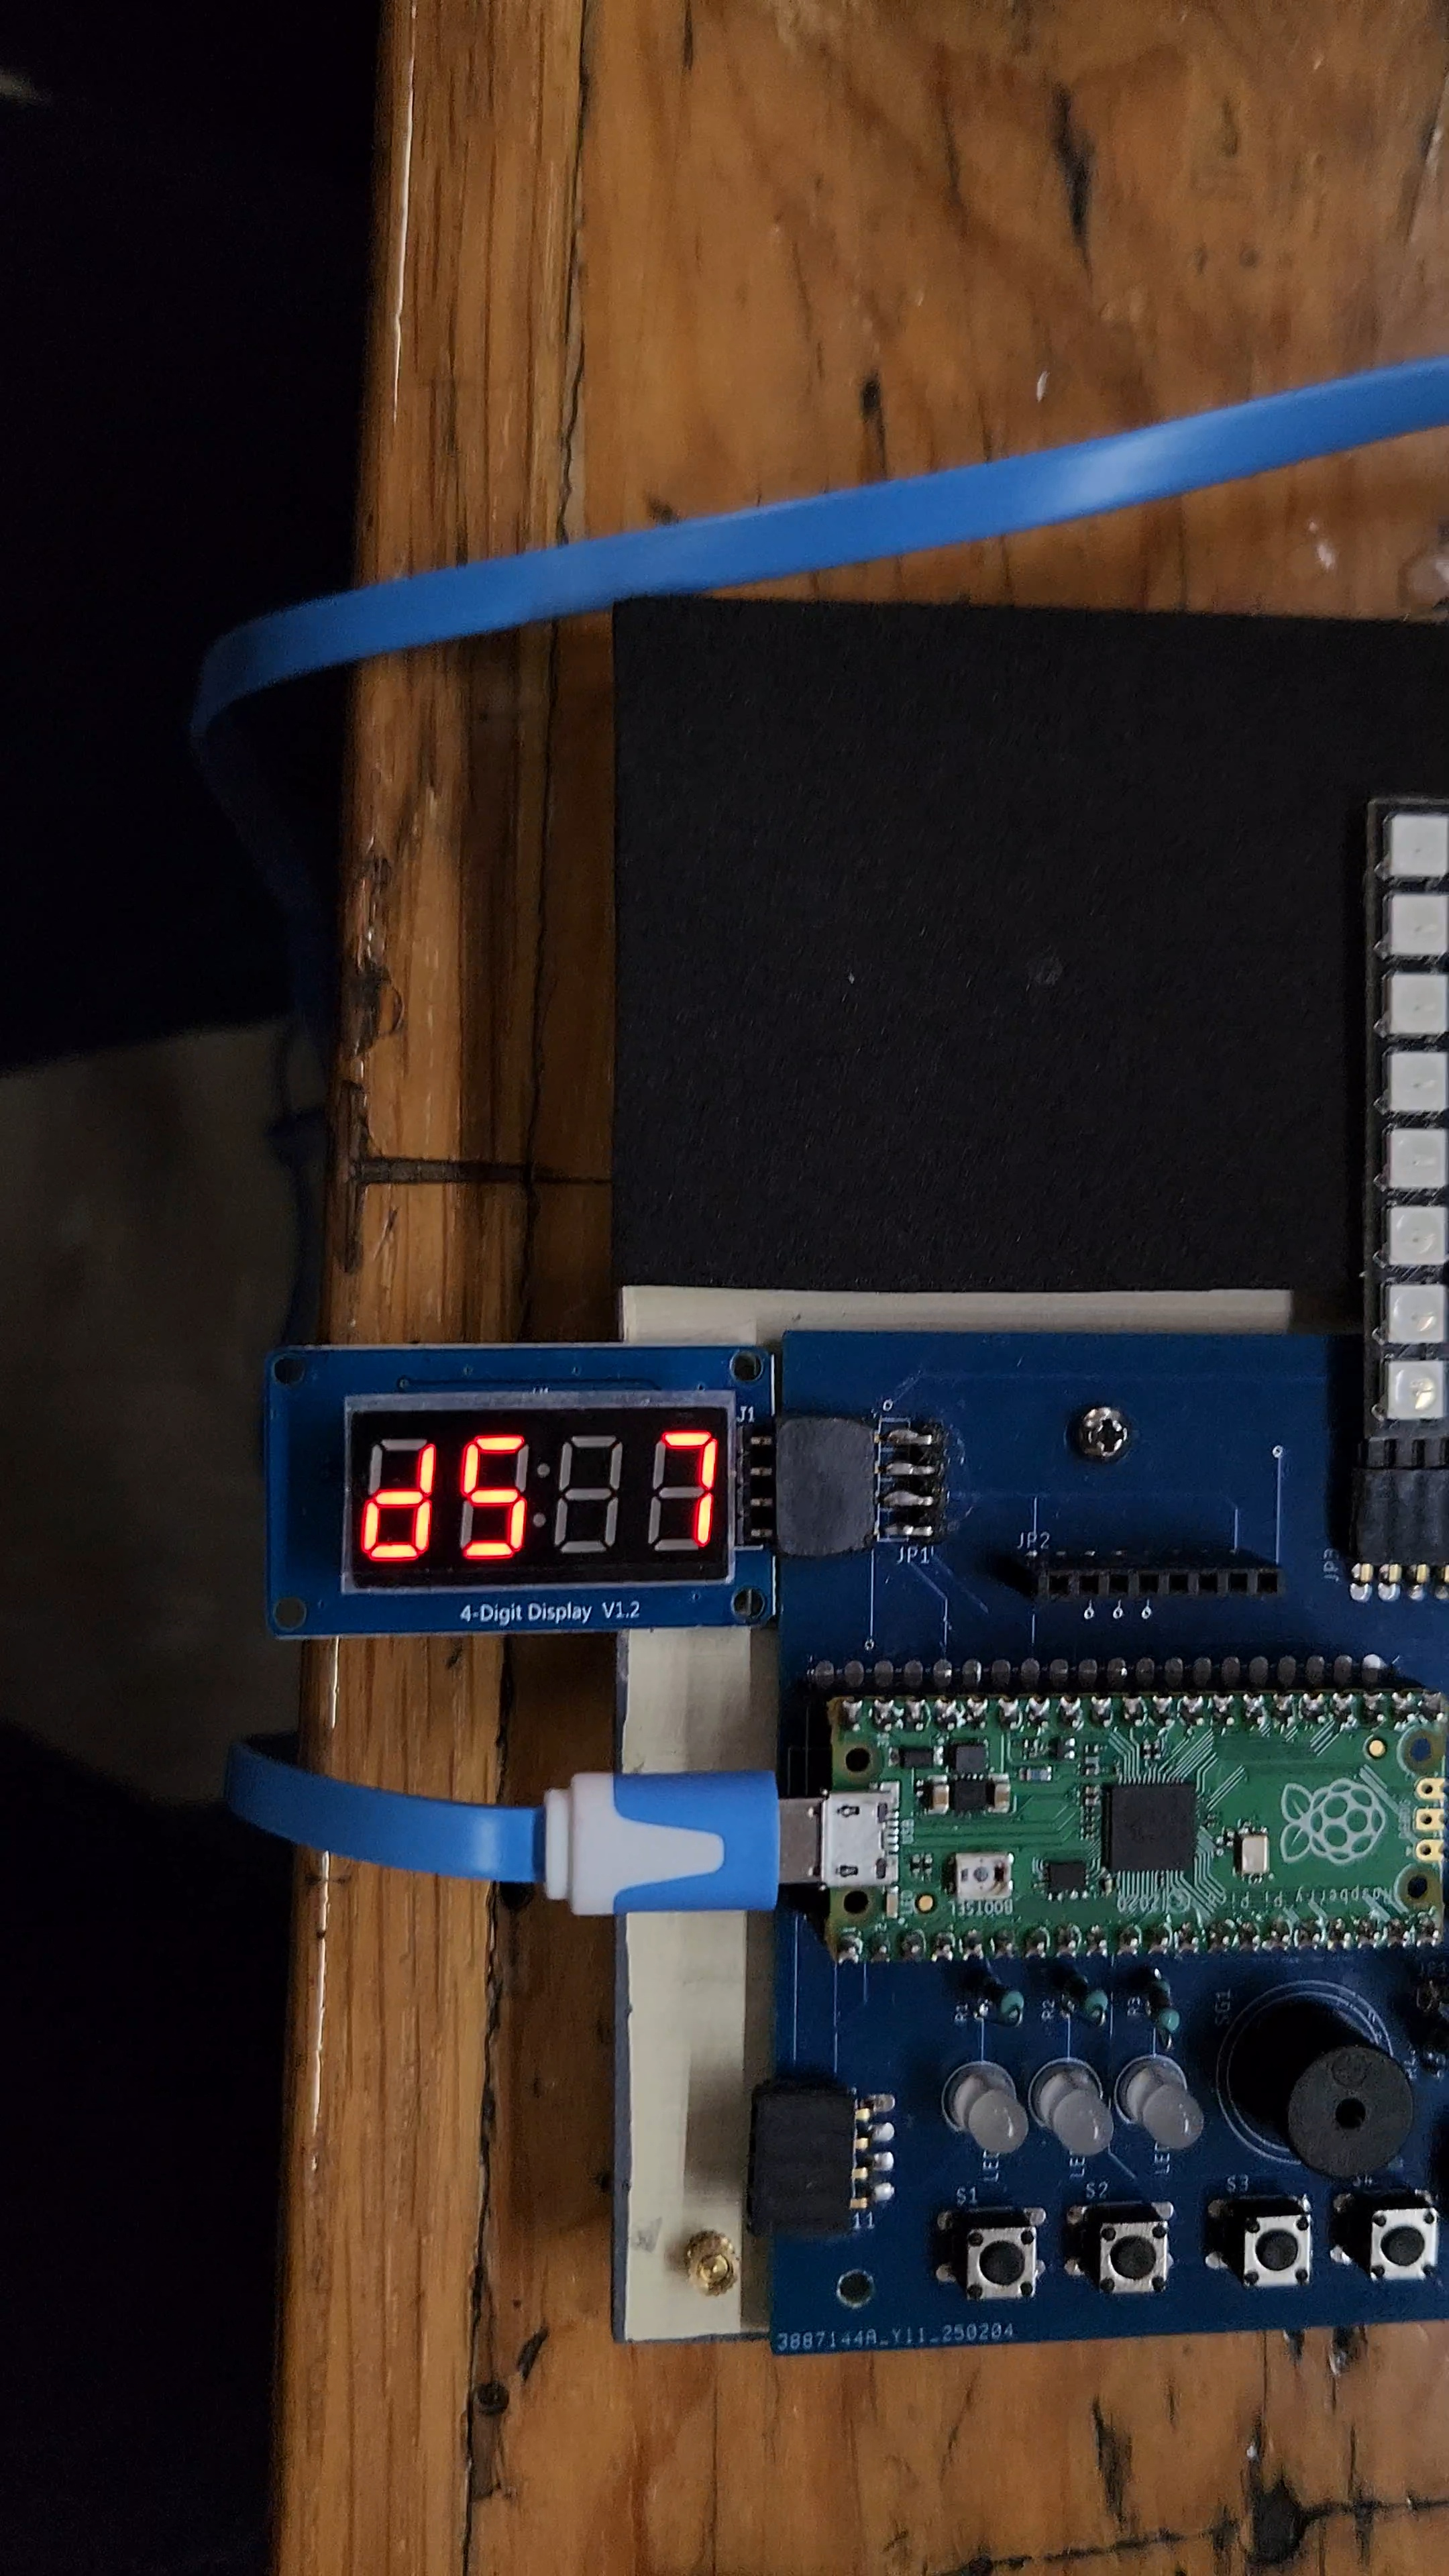
\includegraphics[width=0.4\textwidth, angle=90]{img/Actividad9/Act9_9.jpg}
        \caption{Actualización dinámica del DS18B20. Al aplicarse calor físico al encapsulado, el sensor detecta la variación térmica. El bucle de 10 segundos captura el evento y el display refleja el incremento a "dS 29" de manera continua.}
    \end{figure}

    \begin{figure}[H]
        \centering
        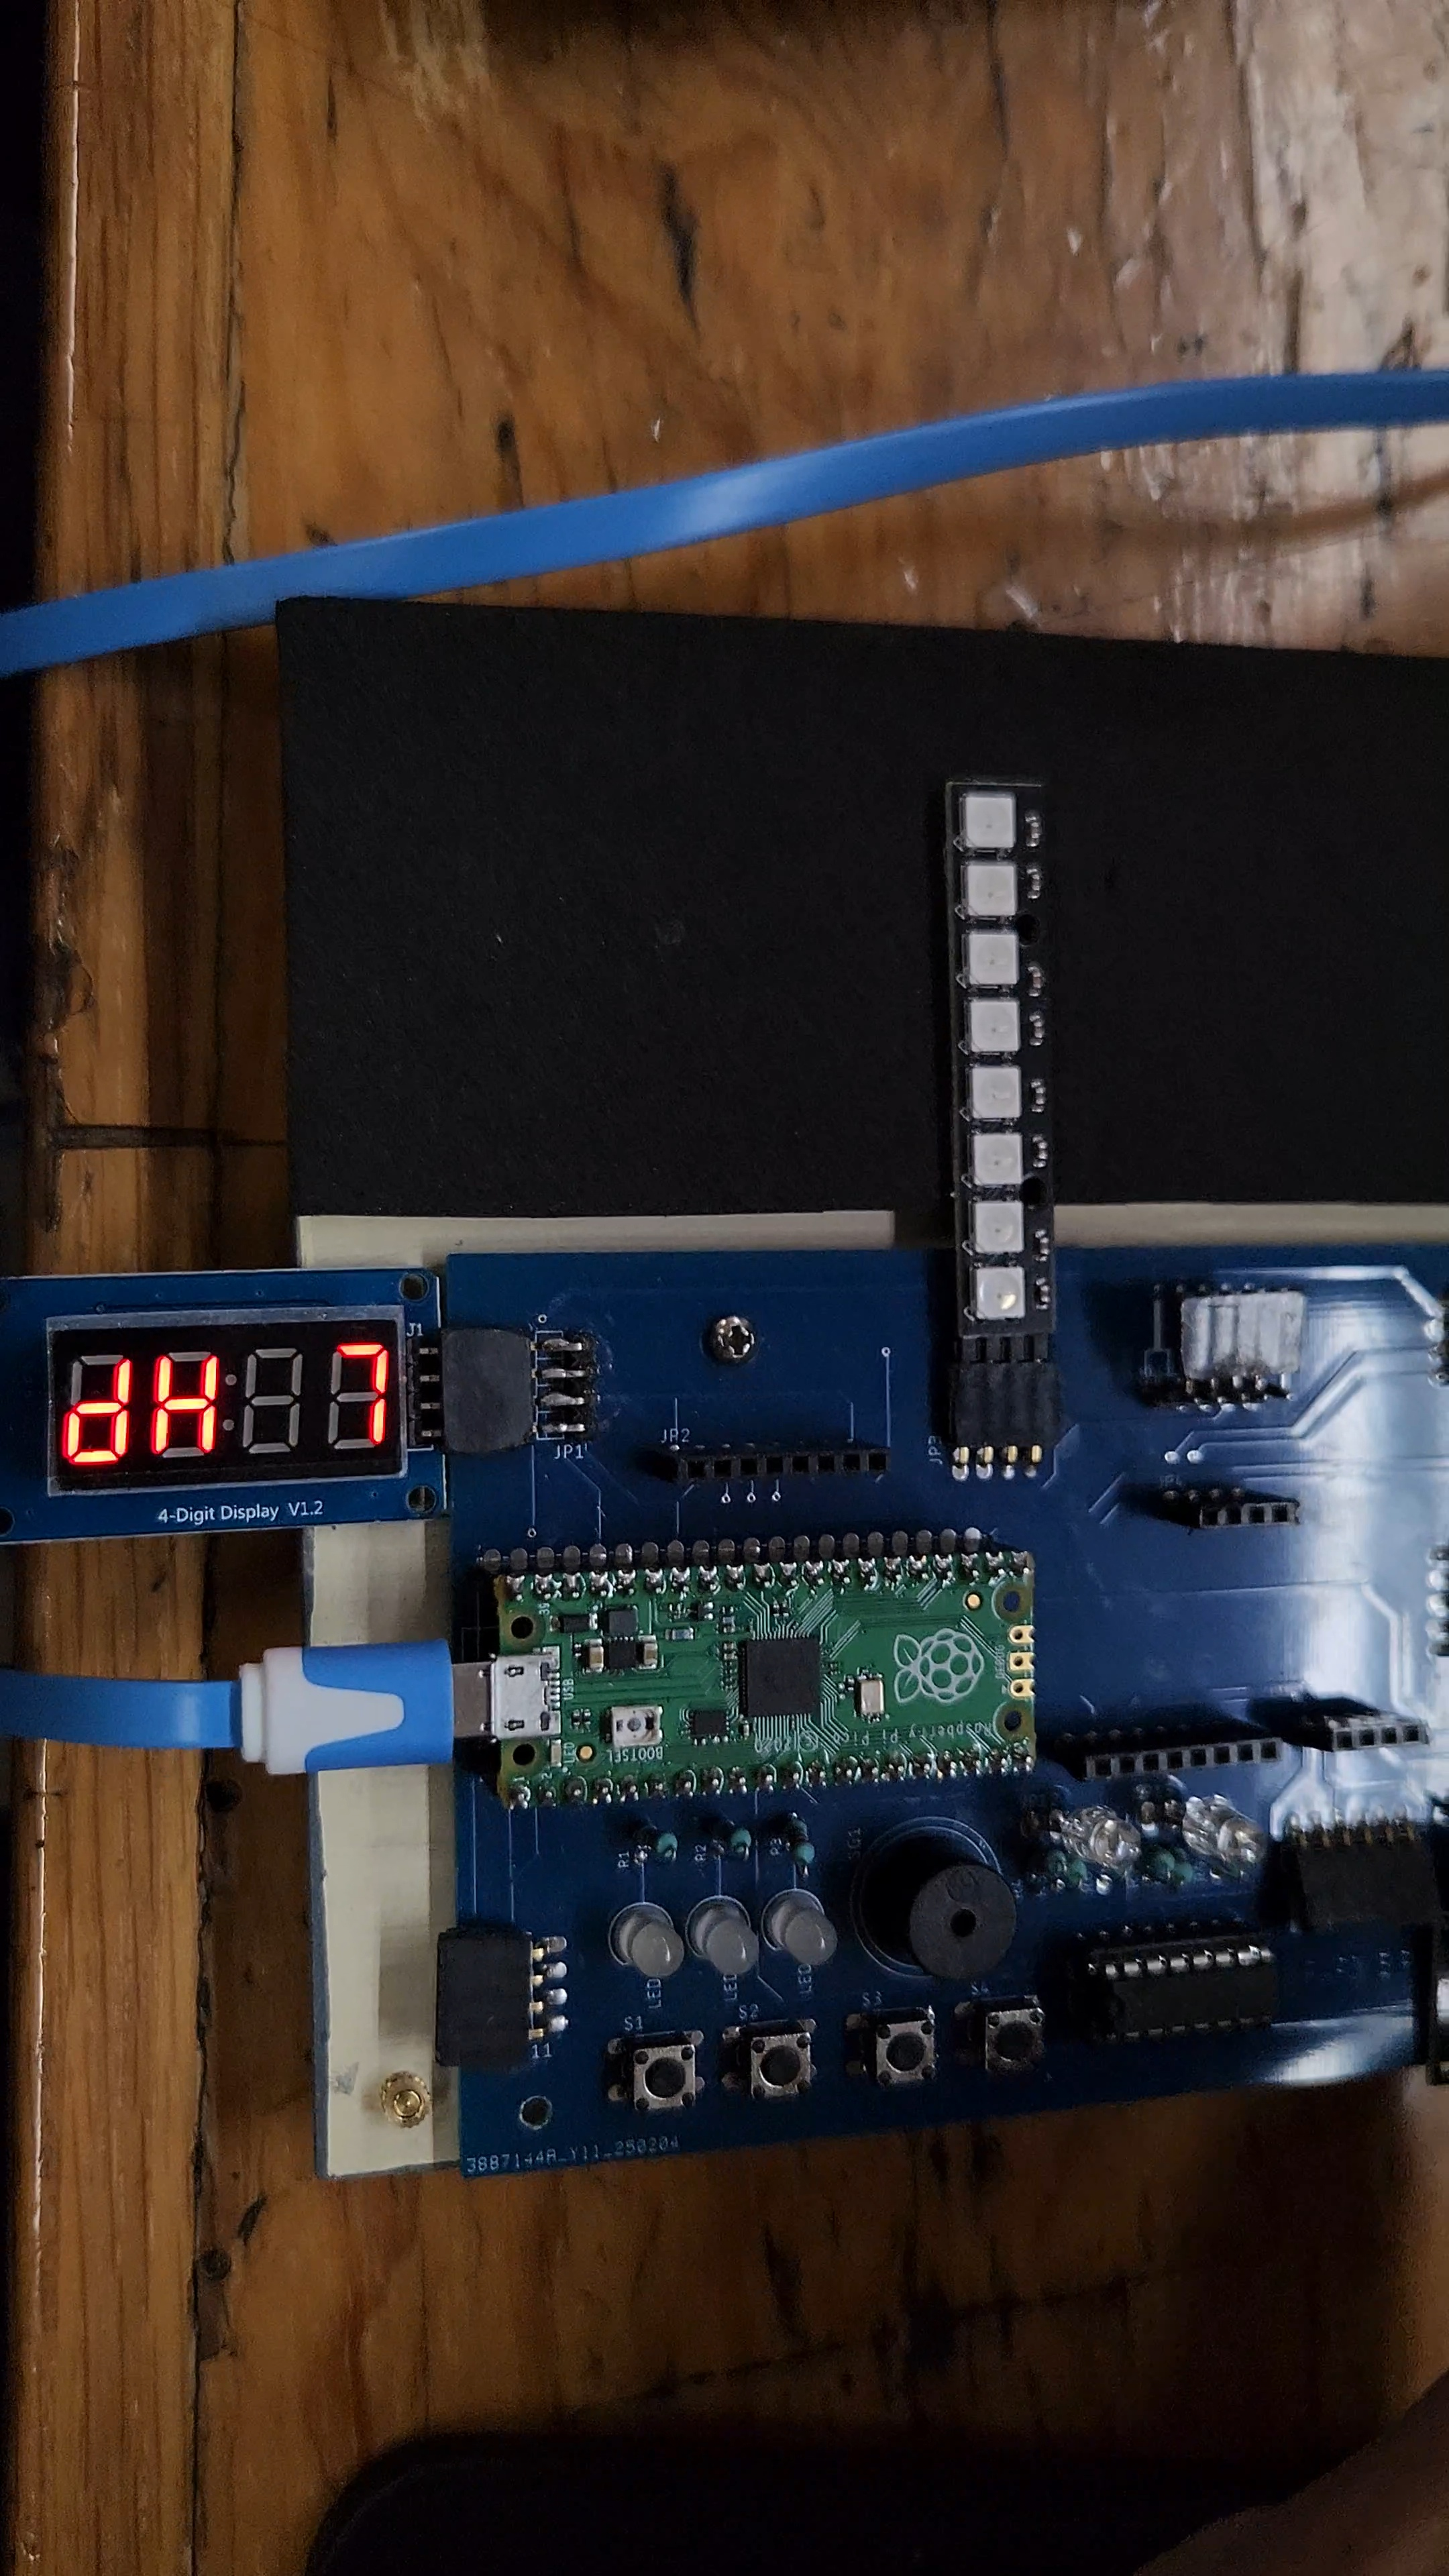
\includegraphics[width=0.4\textwidth, angle=90]{img/Actividad9/Act9_10.jpg}
        \caption{Interrupción por hardware y cambio de modo. Al presionar el botón físico en el GPIO 13, se altera la variable de estado. El flujo principal conmuta al bloque del DHT11 e imprime el prefijo "dH" en la pantalla de 7 segmentos.}
    \end{figure}

    \begin{figure}[H]
        \centering
        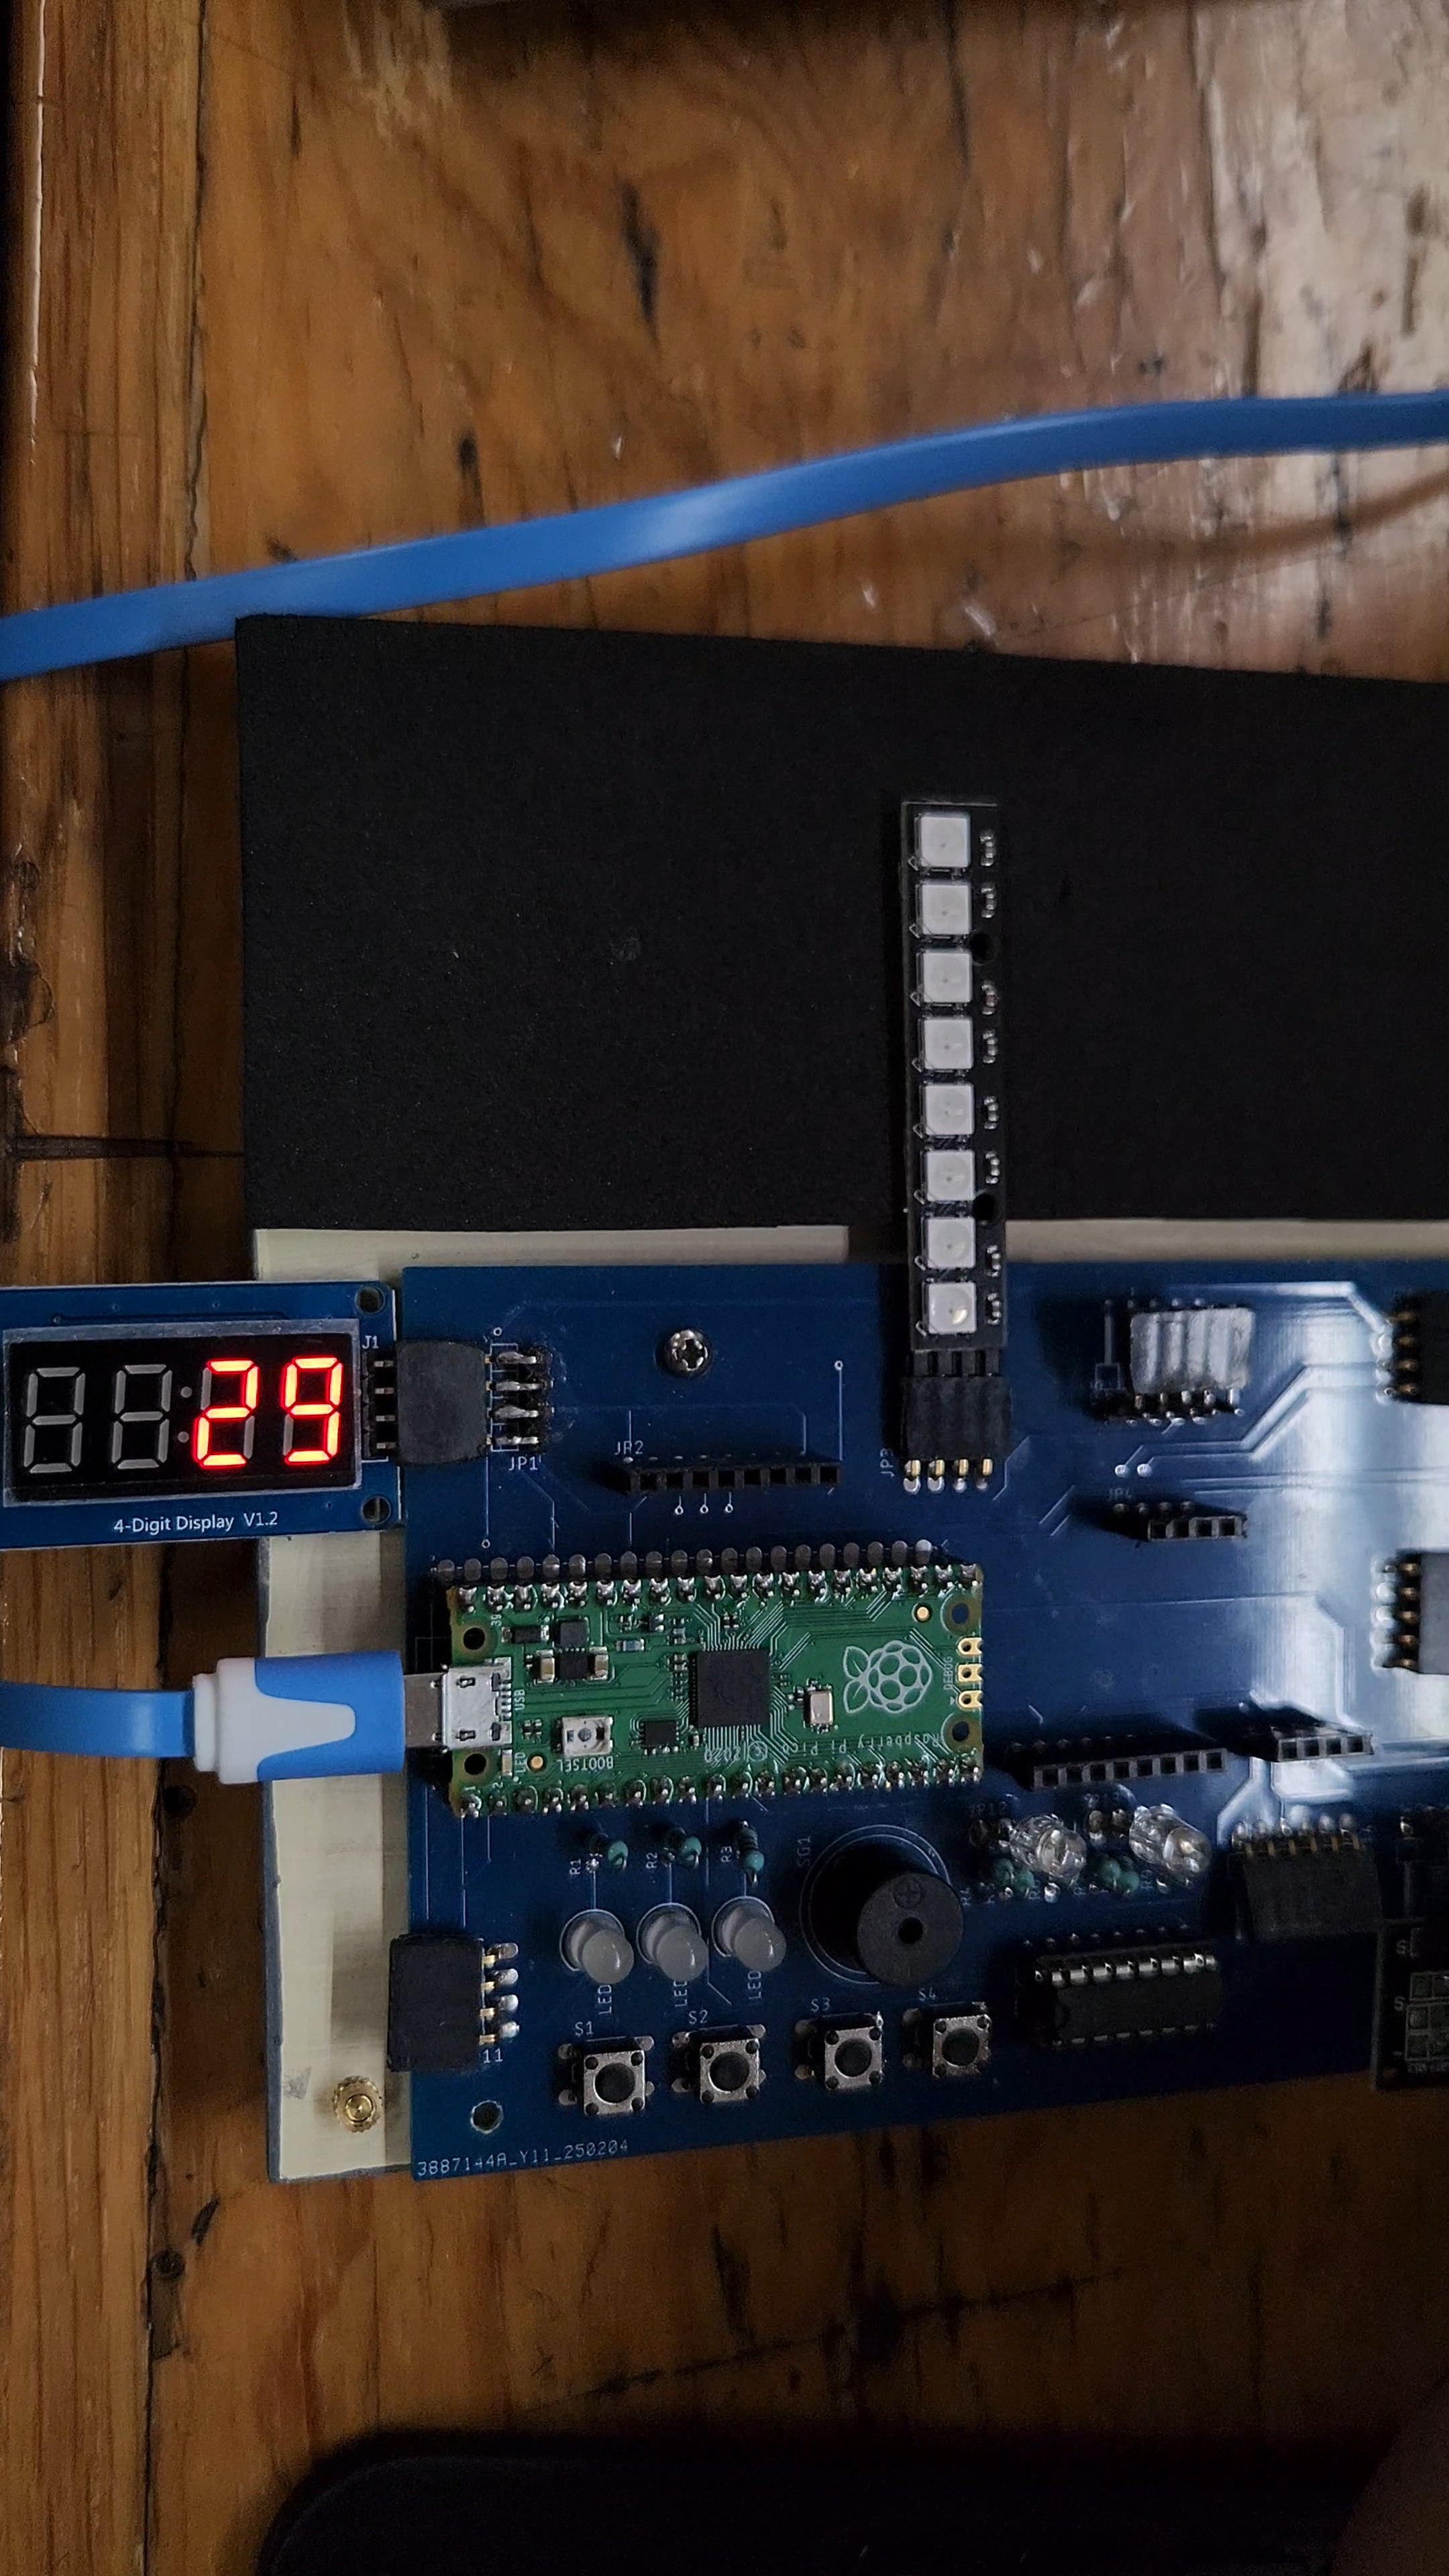
\includegraphics[width=0.4\textwidth, angle=90]{img/Actividad9/Act9_11.jpg}
        \caption{Lectura del segundo sensor.}
    \end{figure}


    \subsection*{Análisis de resultados}
    La ejecución del sistema muestra el manejo concurrente de protocolos muy variados: trenes de pulsos a 800 kHz para los Neopixels, comunicación \textit{1-Wire} para el DS18B20, el protocolo de bus propietario del DHT11 y el protocolo serie del display TM1637. Durante la primera etapa, las funciones de la librería Neopixel aplican las tuplas de color a los LEDs correspondientes, logrando una secuencia de tráfico perfecta y coordinada.

    En la ventana de visualización térmica, resalta la eficiencia en la gestión de sensores. Si la variable de estado corresponde al DS18B20, el microcontrolador respeta la espera necesaria de su conversión analógica, extrae la temperatura y la proyecta en la pantalla anteponiendo temporalmente las letras "DS" para darle contexto visual al usuario. Al presionar el pulsador, la rutina de interrupción cambia el modo. En el siguiente ciclo, el flujo se dirige hacia \texttt{dht\_sensor.measure()}, extrayendo la humedad y temperatura del módulo DHT11 y anteponiendo las letras "DH" en el display. Esta implementación comprueba que es posible integrar dispositivos con requerimientos de sincronización completamente diferentes, unificando sus datos en una sola pantalla mediante el uso inteligente de banderas lógicas e interrupciones.


    \newpage
    \section{Conclusiones:}

    \begin{itemize}
        \item \textbf{Espinoza Matamoros Percival Ulises:} Gracias a la realización de esta práctica logré comprender y aplicar el protocolo de comunicación \textit{One Wire} con el sensor DS18B20, lo que me permitió adquirir datos de temperatura de manera eficiente utilizando un solo pin GPIO, comprendiendo la importancia de este tipo de comunicación, ya se puedeter multiples sensores conectados a un mismo pin, lo que es ideal para proyectos con limitaciones de pines. Por otro lado haciendo uso del display TM1637 pude visualizar los datos obtenidos de manera clara y sencilla, lo que me permitió validar el correcto funcionamiento del sensor y la comunicación. Además, al integrar ambos componentes en un mismo proyecto, pude entender cómo interactúan entre sí y cómo se pueden utilizar juntos para crear soluciones más completas y funcionales.
        
        De forma que el manejo de la raspberry pi pico usando microPython yt las bibliotecas necesarias para cada componente me permitió comprender de mejor forma como es que se realiza la comunicación entre el microcontrolador y los periféricos, por otro lado la sintaxis de microPython me permite comprender la flexbilidad que tienen estos protocolos de comunuicación para distintas aplicaciones en el ámbito de la ingeniería.

        \item \textbf{Flores Colin Victor Jaziel:} En esta practica número nueve logre comprender de manera más completa el manejo de perifericos de salida digital y visualizacion numerica con la Raspberry Pi Pico ya que junto a mi equipo combinamos por ejemplo un display TM1637 y un zumbador pasivo dentro de una misma solucion funcional como en la actividad 4, donde además trabaje con el protocolo I2C simulado (dos hilos: CLK y DIO), actualizando el numero mostrado en cada iteracion con el metodo \texttt{number()} y el uso del zumbador como actuador me permitio incorporar retroalimentacion auditiva al finalizar el conteo, activando el pin GPIO 17 durante exactamente 1 segundo.

        Tambien me ayudo mucho a reforzar el uso de estructuras de control como el bucle \texttt{for} para generar un decremento o incremento automatico para nuestras demás implementaciones para comunicación One Wire que implementamos con la Raspberry Pi Pico y el uso de las librerias Neopixel, tm1637, onewire, ds18x20 y dht de MicroPython.
        
        \item \textbf{Lara Hernandez Angel Husiel:} En esta práctica logré comprender de manera más completa el objetivo del tema de comunicación \textit{One Wire}, porque pasé de usar cada módulo por separado a integrarlos dentro de una misma solución funcional con la Raspberry Pi Pico. Al trabajar con el DS18B20 confirmé cómo se maneja el flujo real de datos en este protocolo: primero la detección del dispositivo en el bus, luego la conversión térmica con su tiempo de espera y finalmente la lectura del dato. Además, al convertir de \textdegree C a \textdegree F y mostrar resultados en consola y display, pude validar que la adquisición y el procesamiento de la información se realizan de forma consistente.

        También me ayudó mucho integrar en un solo programa la lógica de semáforos con Neopixel, el despliegue con TM1637 y la lectura alternada de DS18B20 y DHT11 mediante interrupción por botón.
                
    \end{itemize}

    \newpage


    \nocite{*} 
    \printbibliography[heading=bibintoc, title={Referencias}]

\end{document}